
\documentclass[a4paper,11pt]{article}
\usepackage[a4paper, margin=8em]{geometry}

% usa i pacchetti per la scrittura in italiano
\usepackage[french,italian]{babel}
\usepackage[T1]{fontenc}
\usepackage[utf8]{inputenc}
\frenchspacing 

% usa i pacchetti per la formattazione matematica
\usepackage{amsmath, amssymb, amsthm, amsfonts}

% usa altri pacchetti
\usepackage{gensymb}
\usepackage{hyperref}
\usepackage{standalone}

\usepackage{colortbl}

\usepackage{xstring}
\usepackage{karnaugh-map}

% imposta il titolo
\title{Appunti Calcolatori Elettronici}
\author{Luca Seggiani}
\date{2025}

% imposta lo stile
% usa helvetica
\usepackage[scaled]{helvet}
% usa palatino
\usepackage{palatino}
% usa un font monospazio guardabile
\usepackage{lmodern}

\renewcommand{\rmdefault}{ppl}
\renewcommand{\sfdefault}{phv}
\renewcommand{\ttdefault}{lmtt}

% circuiti
\usepackage{circuitikz}
\usetikzlibrary{babel}

% testo cerchiato
\newcommand*\circled[1]{\tikz[baseline=(char.base)]{
            \node[shape=circle,draw,inner sep=2pt] (char) {#1};}}

% disponi il titolo
\makeatletter
\renewcommand{\maketitle} {
	\begin{center} 
		\begin{minipage}[t]{.8\textwidth}
			\textsf{\huge\bfseries \@title} 
		\end{minipage}%
		\begin{minipage}[t]{.2\textwidth}
			\raggedleft \vspace{-1.65em}
			\textsf{\small \@author} \vfill
			\textsf{\small \@date}
		\end{minipage}
		\par
	\end{center}

	\thispagestyle{empty}
	\pagestyle{fancy}
}
\makeatother

% disponi teoremi
\usepackage{tcolorbox}
\newtcolorbox[auto counter, number within=section]{theorem}[2][]{%
	colback=blue!10, 
	colframe=blue!40!black, 
	sharp corners=northwest,
	fonttitle=\sffamily\bfseries, 
	title=Teorema~\thetcbcounter: #2, 
	#1
}

% disponi definizioni
\newtcolorbox[auto counter, number within=section]{definition}[2][]{%
	colback=red!10,
	colframe=red!40!black,
	sharp corners=northwest,
	fonttitle=\sffamily\bfseries,
	title=Definizione~\thetcbcounter: #2,
	#1
}

% disponi codice
\usepackage{listings}
\usepackage[table]{xcolor}

\definecolor{codegreen}{rgb}{0,0.6,0}
\definecolor{codegray}{rgb}{0.5,0.5,0.5}
\definecolor{codepurple}{rgb}{0.58,0,0.82}
\definecolor{backcolour}{rgb}{0.95,0.95,0.92}

\lstdefinestyle{codestyle}{
		backgroundcolor=\color{black!5}, 
		commentstyle=\color{codegreen},
		keywordstyle=\bfseries\color{magenta},
		numberstyle=\sffamily\tiny\color{black!60},
		stringstyle=\color{green!50!black},
		basicstyle=\ttfamily\footnotesize,
		breakatwhitespace=false,         
		breaklines=true,                 
		captionpos=b,                    
		keepspaces=true,                 
		numbers=left,                    
		numbersep=5pt,                  
		showspaces=false,                
		showstringspaces=false,
		showtabs=false,                  
		tabsize=2
}

\lstdefinestyle{shellstyle}{
		backgroundcolor=\color{black!5}, 
		basicstyle=\ttfamily\footnotesize\color{black}, 
		commentstyle=\color{black}, 
		keywordstyle=\color{black},
		numberstyle=\color{black!5},
		stringstyle=\color{black}, 
		showspaces=false,
		showstringspaces=false, 
		showtabs=false, 
		tabsize=2, 
		numbers=none, 
		breaklines=true
}


\lstdefinelanguage{assembler}{ 
  keywords={AAA, AAD, AAM, AAS, ADC, ADCB, ADCW, ADCL, ADD, ADDB, ADDW, ADDL, AND, ANDB, ANDW, ANDL,
        ARPL, BOUND, BSF, BSFL, BSFW, BSR, BSRL, BSRW, BSWAP, BT, BTC, BTCB, BTCW, BTCL, BTR, 
        BTRB, BTRW, BTRL, BTS, BTSB, BTSW, BTSL, CALL, CBW, CDQ, CLC, CLD, CLI, CLTS, CMC, CMP,
        CMPB, CMPW, CMPL, CMPS, CMPSB, CMPSD, CMPSW, CMPXCHG, CMPXCHGB, CMPXCHGW, CMPXCHGL,
        CMPXCHG8B, CPUID, CWDE, DAA, DAS, DEC, DECB, DECW, DECL, DIV, DIVB, DIVW, DIVL, ENTER,
        HLT, IDIV, IDIVB, IDIVW, IDIVL, IMUL, IMULB, IMULW, IMULL, IN, INB, INW, INL, INC, INCB,
        INCW, INCL, INS, INSB, INSD, INSW, INT, INT3, INTO, INVD, INVLPG, IRET, IRETD, JA, JAE,
        JB, JBE, JC, JCXZ, JE, JECXZ, JG, JGE, JL, JLE, JMP, JNA, JNAE, JNB, JNBE, JNC, JNE, JNG,
        JNGE, JNL, JNLE, JNO, JNP, JNS, JNZ, JO, JP, JPE, JPO, JS, JZ, LAHF, LAR, LCALL, LDS,
        LEA, LEAVE, LES, LFS, LGDT, LGS, LIDT, LMSW, LOCK, LODSB, LODSD, LODSW, LOOP, LOOPE,
        LOOPNE, LSL, LSS, LTR, MOV, MOVB, MOVW, MOVL, MOVSB, MOVSD, MOVSW, MOVSX, MOVSXB,
        MOVSXW, MOVSXL, MOVZX, MOVZXB, MOVZXW, MOVZXL, MUL, MULB, MULW, MULL, NEG, NEGB, NEGW,
        NEGL, NOP, NOT, NOTB, NOTW, NOTL, OR, ORB, ORW, ORL, OUT, OUTB, OUTW, OUTL, OUTSB, OUTSD,
        OUTSW, POP, POPL, POPW, POPB, POPA, POPAD, POPF, POPFD, PUSH, PUSHL, PUSHW, PUSHB, PUSHA, 
				PUSHAD, PUSHF, PUSHFD, RCL, RCLB, RCLW, MOVSL, MOVSB, MOVSW, STOSL, STOSB, STOSW, LODSB, LODSW,
				LODSL, INSB, INSW, INSL, OUTSB, OUTSL, OUTSW
        RCLL, RCR, RCRB, RCRW, RCRL, RDMSR, RDPMC, RDTSC, REP, REPE, REPNE, RET, ROL, ROLB, ROLW,
        ROLL, ROR, RORB, RORW, RORL, SAHF, SAL, SALB, SALW, SALL, SAR, SARB, SARW, SARL, SBB,
        SBBB, SBBW, SBBL, SCASB, SCASD, SCASW, SETA, SETAE, SETB, SETBE, SETC, SETE, SETG, SETGE,
        SETL, SETLE, SETNA, SETNAE, SETNB, SETNBE, SETNC, SETNE, SETNG, SETNGE, SETNL, SETNLE,
        SETNO, SETNP, SETNS, SETNZ, SETO, SETP, SETPE, SETPO, SETS, SETZ, SGDT, SHL, SHLB, SHLW,
        SHLL, SHLD, SHR, SHRB, SHRW, SHRL, SHRD, SIDT, SLDT, SMSW, STC, STD, STI, STOSB, STOSD,
        STOSW, STR, SUB, SUBB, SUBW, SUBL, TEST, TESTB, TESTW, TESTL, VERR, VERW, WAIT, WBINVD,
        XADD, XADDB, XADDW, XADDL, XCHG, XCHGB, XCHGW, XCHGL, XLAT, XLATB, XOR, XORB, XORW, XORL},
  keywordstyle=\color{blue}\bfseries,
  ndkeywordstyle=\color{darkgray}\bfseries,
  identifierstyle=\color{black},
  sensitive=false,
  comment=[l]{\#},
  morecomment=[s]{/*}{*/},
  commentstyle=\color{purple}\ttfamily,
  stringstyle=\color{red}\ttfamily,
  morestring=[b]',
  morestring=[b]"
}

\lstset{language=assembler, style=codestyle}

% disponi sezioni
\usepackage{titlesec}

\titleformat{\section}
	{\sffamily\Large\bfseries} 
	{\thesection}{1em}{} 
\titleformat{\subsection}
	{\sffamily\large\bfseries}   
	{\thesubsection}{1em}{} 
\titleformat{\subsubsection}
	{\sffamily\normalsize\bfseries} 
	{\thesubsubsection}{1em}{}

% tikz
\usepackage{tikz}

% float
\usepackage{float}

% grafici
\usepackage{pgfplots}
\pgfplotsset{width=10cm,compat=1.9}

% disponi alberi
\usepackage{forest}

\forestset{
	rectstyle/.style={
		for tree={rectangle,draw,font=\large\sffamily}
	},
	roundstyle/.style={
		for tree={circle,draw,font=\large}
	}
}

% disponi algoritmi
\usepackage{algorithm}
\usepackage{algorithmic}
\makeatletter
\renewcommand{\ALG@name}{Algoritmo}
\makeatother

% disponi numeri di pagina
\usepackage{fancyhdr}
\fancyhf{} 
\fancyfoot[L]{\sffamily{\thepage}}

\makeatletter
\fancyhead[L]{\raisebox{1ex}[0pt][0pt]{\sffamily{\@title \ \@date}}} 
\fancyhead[R]{\raisebox{1ex}[0pt][0pt]{\sffamily{\@author}}}
\makeatother

\begin{document}

\pagestyle{fancy}
\thispagestyle{empty}
\renewcommand{\thispagestyle}[1]{}

\maketitle

\documentclass[a4paper,11pt]{article}
\usepackage[a4paper, margin=8em]{geometry}

% usa i pacchetti per la scrittura in italiano
\usepackage[french,italian]{babel}
\usepackage[T1]{fontenc}
\usepackage[utf8]{inputenc}
\frenchspacing 

% usa i pacchetti per la formattazione matematica
\usepackage{amsmath, amssymb, amsthm, amsfonts}

% usa altri pacchetti
\usepackage{gensymb}
\usepackage{hyperref}
\usepackage{standalone}

\usepackage{colortbl}

\usepackage{xstring}
\usepackage{karnaugh-map}

% imposta il titolo
\title{Appunti Calcolatori Elettronici}
\author{Luca Seggiani}
\date{2025}

% imposta lo stile
% usa helvetica
\usepackage[scaled]{helvet}
% usa palatino
\usepackage{palatino}
% usa un font monospazio guardabile
\usepackage{lmodern}

\renewcommand{\rmdefault}{ppl}
\renewcommand{\sfdefault}{phv}
\renewcommand{\ttdefault}{lmtt}

% circuiti
\usepackage{circuitikz}
\usetikzlibrary{babel}

% testo cerchiato
\newcommand*\circled[1]{\tikz[baseline=(char.base)]{
            \node[shape=circle,draw,inner sep=2pt] (char) {#1};}}

% disponi il titolo
\makeatletter
\renewcommand{\maketitle} {
	\begin{center} 
		\begin{minipage}[t]{.8\textwidth}
			\textsf{\huge\bfseries \@title} 
		\end{minipage}%
		\begin{minipage}[t]{.2\textwidth}
			\raggedleft \vspace{-1.65em}
			\textsf{\small \@author} \vfill
			\textsf{\small \@date}
		\end{minipage}
		\par
	\end{center}

	\thispagestyle{empty}
	\pagestyle{fancy}
}
\makeatother

% disponi teoremi
\usepackage{tcolorbox}
\newtcolorbox[auto counter, number within=section]{theorem}[2][]{%
	colback=blue!10, 
	colframe=blue!40!black, 
	sharp corners=northwest,
	fonttitle=\sffamily\bfseries, 
	title=Teorema~\thetcbcounter: #2, 
	#1
}

% disponi definizioni
\newtcolorbox[auto counter, number within=section]{definition}[2][]{%
	colback=red!10,
	colframe=red!40!black,
	sharp corners=northwest,
	fonttitle=\sffamily\bfseries,
	title=Definizione~\thetcbcounter: #2,
	#1
}

% disponi codice
\usepackage{listings}
\usepackage[table]{xcolor}

\definecolor{codegreen}{rgb}{0,0.6,0}
\definecolor{codegray}{rgb}{0.5,0.5,0.5}
\definecolor{codepurple}{rgb}{0.58,0,0.82}
\definecolor{backcolour}{rgb}{0.95,0.95,0.92}

\lstdefinestyle{codestyle}{
		backgroundcolor=\color{black!5}, 
		commentstyle=\color{codegreen},
		keywordstyle=\bfseries\color{magenta},
		numberstyle=\sffamily\tiny\color{black!60},
		stringstyle=\color{green!50!black},
		basicstyle=\ttfamily\footnotesize,
		breakatwhitespace=false,         
		breaklines=true,                 
		captionpos=b,                    
		keepspaces=true,                 
		numbers=left,                    
		numbersep=5pt,                  
		showspaces=false,                
		showstringspaces=false,
		showtabs=false,                  
		tabsize=2
}

\lstdefinestyle{shellstyle}{
		backgroundcolor=\color{black!5}, 
		basicstyle=\ttfamily\footnotesize\color{black}, 
		commentstyle=\color{black}, 
		keywordstyle=\color{black},
		numberstyle=\color{black!5},
		stringstyle=\color{black}, 
		showspaces=false,
		showstringspaces=false, 
		showtabs=false, 
		tabsize=2, 
		numbers=none, 
		breaklines=true
}


\lstdefinelanguage{assembler}{ 
  keywords={AAA, AAD, AAM, AAS, ADC, ADCB, ADCW, ADCL, ADD, ADDB, ADDW, ADDL, AND, ANDB, ANDW, ANDL,
        ARPL, BOUND, BSF, BSFL, BSFW, BSR, BSRL, BSRW, BSWAP, BT, BTC, BTCB, BTCW, BTCL, BTR, 
        BTRB, BTRW, BTRL, BTS, BTSB, BTSW, BTSL, CALL, CBW, CDQ, CLC, CLD, CLI, CLTS, CMC, CMP,
        CMPB, CMPW, CMPL, CMPS, CMPSB, CMPSD, CMPSW, CMPXCHG, CMPXCHGB, CMPXCHGW, CMPXCHGL,
        CMPXCHG8B, CPUID, CWDE, DAA, DAS, DEC, DECB, DECW, DECL, DIV, DIVB, DIVW, DIVL, ENTER,
        HLT, IDIV, IDIVB, IDIVW, IDIVL, IMUL, IMULB, IMULW, IMULL, IN, INB, INW, INL, INC, INCB,
        INCW, INCL, INS, INSB, INSD, INSW, INT, INT3, INTO, INVD, INVLPG, IRET, IRETD, JA, JAE,
        JB, JBE, JC, JCXZ, JE, JECXZ, JG, JGE, JL, JLE, JMP, JNA, JNAE, JNB, JNBE, JNC, JNE, JNG,
        JNGE, JNL, JNLE, JNO, JNP, JNS, JNZ, JO, JP, JPE, JPO, JS, JZ, LAHF, LAR, LCALL, LDS,
        LEA, LEAVE, LES, LFS, LGDT, LGS, LIDT, LMSW, LOCK, LODSB, LODSD, LODSW, LOOP, LOOPE,
        LOOPNE, LSL, LSS, LTR, MOV, MOVB, MOVW, MOVL, MOVSB, MOVSD, MOVSW, MOVSX, MOVSXB,
        MOVSXW, MOVSXL, MOVZX, MOVZXB, MOVZXW, MOVZXL, MUL, MULB, MULW, MULL, NEG, NEGB, NEGW,
        NEGL, NOP, NOT, NOTB, NOTW, NOTL, OR, ORB, ORW, ORL, OUT, OUTB, OUTW, OUTL, OUTSB, OUTSD,
        OUTSW, POP, POPL, POPW, POPB, POPA, POPAD, POPF, POPFD, PUSH, PUSHL, PUSHW, PUSHB, PUSHA, 
				PUSHAD, PUSHF, PUSHFD, RCL, RCLB, RCLW, MOVSL, MOVSB, MOVSW, STOSL, STOSB, STOSW, LODSB, LODSW,
				LODSL, INSB, INSW, INSL, OUTSB, OUTSL, OUTSW
        RCLL, RCR, RCRB, RCRW, RCRL, RDMSR, RDPMC, RDTSC, REP, REPE, REPNE, RET, ROL, ROLB, ROLW,
        ROLL, ROR, RORB, RORW, RORL, SAHF, SAL, SALB, SALW, SALL, SAR, SARB, SARW, SARL, SBB,
        SBBB, SBBW, SBBL, SCASB, SCASD, SCASW, SETA, SETAE, SETB, SETBE, SETC, SETE, SETG, SETGE,
        SETL, SETLE, SETNA, SETNAE, SETNB, SETNBE, SETNC, SETNE, SETNG, SETNGE, SETNL, SETNLE,
        SETNO, SETNP, SETNS, SETNZ, SETO, SETP, SETPE, SETPO, SETS, SETZ, SGDT, SHL, SHLB, SHLW,
        SHLL, SHLD, SHR, SHRB, SHRW, SHRL, SHRD, SIDT, SLDT, SMSW, STC, STD, STI, STOSB, STOSD,
        STOSW, STR, SUB, SUBB, SUBW, SUBL, TEST, TESTB, TESTW, TESTL, VERR, VERW, WAIT, WBINVD,
        XADD, XADDB, XADDW, XADDL, XCHG, XCHGB, XCHGW, XCHGL, XLAT, XLATB, XOR, XORB, XORW, XORL},
  keywordstyle=\color{blue}\bfseries,
  ndkeywordstyle=\color{darkgray}\bfseries,
  identifierstyle=\color{black},
  sensitive=false,
  comment=[l]{\#},
  morecomment=[s]{/*}{*/},
  commentstyle=\color{purple}\ttfamily,
  stringstyle=\color{red}\ttfamily,
  morestring=[b]',
  morestring=[b]"
}

\lstset{language=assembler, style=codestyle}

% disponi sezioni
\usepackage{titlesec}

\titleformat{\section}
	{\sffamily\Large\bfseries} 
	{\thesection}{1em}{} 
\titleformat{\subsection}
	{\sffamily\large\bfseries}   
	{\thesubsection}{1em}{} 
\titleformat{\subsubsection}
	{\sffamily\normalsize\bfseries} 
	{\thesubsubsection}{1em}{}

% tikz
\usepackage{tikz}

% float
\usepackage{float}

% grafici
\usepackage{pgfplots}
\pgfplotsset{width=10cm,compat=1.9}

% disponi alberi
\usepackage{forest}

\forestset{
	rectstyle/.style={
		for tree={rectangle,draw,font=\large\sffamily}
	},
	roundstyle/.style={
		for tree={circle,draw,font=\large}
	}
}

% disponi algoritmi
\usepackage{algorithm}
\usepackage{algorithmic}
\makeatletter
\renewcommand{\ALG@name}{Algoritmo}
\makeatother

% disponi numeri di pagina
\usepackage{fancyhdr}
\fancyhf{} 
\fancyfoot[L]{\sffamily{\thepage}}

\makeatletter
\fancyhead[L]{\raisebox{1ex}[0pt][0pt]{\sffamily{\@title \ \@date}}} 
\fancyhead[R]{\raisebox{1ex}[0pt][0pt]{\sffamily{\@author}}}
\makeatother

\begin{document}
% sezione (data)
\section{Lezione del 24-02-25}

% stili pagina
\thispagestyle{empty}
\pagestyle{fancy}

% testo
\subsection{Introduzione al corso}
Continuiamo lo studio di una particolare architettura per calcolatori, a partire da quanto detto riguardo alle reti logiche, introducendo i concetti di \textbf{interruzione}, \textbf{protezione} e \textbf{memoria virtuale}.
Questi 3 strumenti ci permetterano di realizzare il paradigma della \textbf{multiprogrammazione}, cioè di far eseguire ad una macchina con un singolo processore più programmi contemporaneamente.
Non si pensi questo significhi avere più processori, in quanto il corso riguarda esclusivamente processori \textit{single-threading}.

\subsection{Architettura}
L'archittettura di riferimento è quella classica, composta da \textbf{CPU}, \textbf{memoria} e \textbf{I/O} interconnessi da un \textbf{bus}.

Durante lo studio di un archiettura è oppurtuno porsi la domanda \textit{"chi fa cosa?"}, che fornisce determinati \textit{chi} ai determinati \textit{cosa} forniti da un opportuno livello di astrazione (transistor, porte logiche, diagrammi funzionali, ecc...).

La domanda che potremo porci adesso è \textit{"chi comanda?"} all'interno dell'architettura vista.
La risposta più giusta è quella del \textbf{software}: l'architettura è fatta per \textit{eseguire} software.

Per convincerci di questo possiamo sostituire la domanda \textit{"chi fa cosa?"} con la domanda \textit{"chi sa cosa?"}.

\begin{itemize}
	\item 
La \textbf{CPU} conosce lo stato corrente dei registri e l'istruzione in esecuzione.
Fra un'istruzione e l'altra non c'è alcun bisogno di sapere cosa è accaduto finora, e cosa accadrà in futuro, ma solamente l'istruzione corrente.
Quindi si può pensare che la CPU non \textit{sa} qual'è l'obiettivo della computazione, ma si limita a portarla avanti.

	\item
La \textbf{memoria} è un oggetto passivo, che contiene il programma, ma si limita a restiture i dati richiesti quando sono richiesti.
Notiamo che le memorie che usiamo sono ad \textbf{accesso casuale}, ergo nessuno scorre alla ricerca di indirizzi, ma si può leggere e scrivere in posizioni arbitrarie in tempo pressoché costante.
La memoria contiene \textbf{sempre} qualcosa, che questo sia significativo o meno, e la sua tipizzazione dipende solamente dalle intenzioni del programmatore.
	
	\item
L'\textbf{I/O} è il componente più variegato dell'architettura.
L'unica costante che rende la comunicazione con le periferiche più facile è la presenza di un interfaccia, che riduce tale comunicazione ad una semplice lettura o scrittura nello spazio di I/O.
La differenza fra le letture e scritture nello spazio di I/O e lo spazio di memoria è la possibile presenza di \textbf{effetti collaterali}, cioè effetti non riconducibili alla sola variazione di stato di una locazione di memoria.
Inoltre la CPU non è l'unica a scrivere nello spazio di I/O, in quanto questo può essere fatto anche dalle periferiche stesse.

	\item
Il \textbf{bus} è un insieme di linee (\textit{fili}), che trasportano ciò che ogni componente sta comunicando in un dato momento.
Ogni componente vede ciò che viene scritto sul bus in qualsiasi momento, e l'indirizzamento di locazioni specifiche nello spazio di memoria o nello spazio di I/O viene fatto attraverso \textbf{maschere} di indirizzo. 
\end{itemize}

\subsubsection{Flusso di controllo}
Abbiamo visto come la CPU si limita a prelevare ed eseguire istruzioni nel ciclo di \textbf{fetch-execute}.
L'istruzione successiva alla corrente, il cui indirizzo viene scritto nell'\textbf{instruction pointer}, viene decisa dall'istruzione corrente stessa (si pensi alle istruzioni di salto).
Il \textbf{flusso di controllo} è quindi deciso dall istruzioni stesse, cioè dal programma.

\subsubsection{Bootstrap}
Il \textbf{bootstrap} è un processo secondo il quale si porta il sistema in un certo stato di esecuzione, apparentemente impossibile, o comunque molto difficile, da raggiungere.
Ad esempio, il compilatore del linguaggio C è scritto esso stesso in linguaggio C.
La domanda naturale è \textit{"come è stato compilato il compilatore?"}.
La risposta è un processo di boostrap, usando o un compilatore presesistente, magari che implementa un sottoinsieme parziale del C, o scrivendo l'intero compilatore in linguaggio macchina, cioè assemblando codice assembler.

Il boostrap si rende necessario anche all'avvio del calcolatore, per il caricamento del programma all'interno della memoria e l'inizio dell'esecuzione.
Nei calcolatori moderni questo viene fatto attraverso la \textbf{ROM}, cioè una memoria a sola lettura che contiene un programma di bootstrap.
All'avvio il processore è impostato in modo che al reset prenda come indirizzo proprio quello della ROM, e quindi inizi ad eseguire il programma di boostrap.
All'interno della ROM si trova, nei calcolatori moderni, il \textbf{BIOS} (o \textit{UEFI}, nei sistemi moderni), che ha il solo compito di impostare alcune periferiche di base e caricare il sistema operativo.

\par\medskip 

Iniziamo quindi ad approfondire, uno per uno, i moduli dell'architettura.

\subsection{Memoria}
La memoria è un insieme contiguo di locazioni di memoria, che nelle architetture moderne sono rappresentate da byte.
Storicamente, la memoria era indirizzata a \textit{parole}, cioè insiemi di bit coincidenti in dimensioni coi registri del processore.
Una parola poteva essere di più byte, mentre oggi le memorie sono accessibili ai singoli byte.
Ad esempio, le memorie usate nell'architettura Intel x86 sono accessibili ad 1 byte (\lstinline|MOVB|), 2 byte (\lstinline|MOVW|), 4 byte (\lstinline|MOVL|), e 8 byte (\lstinline|MOVQ|).

\subsubsection{Endianess}
Notiamo che la posizione in memoria del byte più significativo di una parola (in questo caso consideriamo una "parola" da 8 byte, da cui si ricavano tutte le altre misure) determina l'\textit{endianess} dell'architettura.
In particolare, se l'ultimo byte sta in fondo nella memoria, si dice \textbf{big-endian}, mentre se viceversa l'ultimo byte viene per primo nella memoria, si dice \textbf{little-endian}.

L'architettura Intel x86 che andiamo a considerare è little-endian, come lo sono la maggior parte delle architetture moderne.
Un esempio di utilizzo del big-endian e nella trasmissione di dati attraverso il protocollo IP, usato nelle comunicazioni Internet.

\subsubsection{Allineamento}
Indicheremo con \textbf{offset} la distanza in byte fra due locazioni di memoria, inteso come il numero di locazioni che vanno saltate per raggiungere un indirizzo a partire dall'altro.
In questo ha senso parlare anche di offset \textit{negativi}.

Visto che lo spazio di memoria è effettivamente ciclico, cioò si ha \textit{wrap-around} ai suoi capi, si ha che gli offset rimangono validi \textbf{modulo} la dimensione dello spazio di memoria, che è sempre $2^n$, con $n$ nel nostro caso uguale a 64.

Il \textit{wrap-around} si comporta bene con gli offset, ma lo stesso non si può dire per quanto riguarda \textbf{intervalli} di byte.
Preso un certo intervallo $[x, y)$, quindi, si ha che questo contiene gli indirizzi $\{n \, | \, x \leq n < y\}$, ammesso che $x < y$, cosa che risulta falsa nel caso di intervalli che hanno \textit{wrap-around}. 
Decidiamo di non considerare intervalli di questo tipo.
Questo rende necessaria un'eccezione per intervalli che comprendono l'ultimo byte: in questo caso è concesso $[x, 0)$, con 0 che indica il fondo dello spazio di memoria.

Veniamo quindi all'\textbf{allineamento}.
Dire che un indirizzo è allineato ad un numero $n$ significa dire che quell'indirizzo è un multiplo di $n$.
Chiaramente, conviene scegliere $n$ potenze di 2.
In questo caso, per riconoscere se un indirizzo è allineato a $2^k$, basta guardare i suoi primi $k$ bit.

Si dice spesso che oggetti sono \textit{allineati alla parola}, ecc...
Questo significa che sono allineati alla \textit{dimensione} della parola specificata.
Altrimenti, si può dire che un oggetto è allineato \textit{naturalmente}, nel caso in cui sia allineato alla dimensione di stesso.

Infine, il \textbf{confine} di un oggetto è l'indirizzo che lo delimita dal resto dello spazio di memoria.

\end{document}


\documentclass[a4paper,11pt]{article}
\usepackage[a4paper, margin=8em]{geometry}

% usa i pacchetti per la scrittura in italiano
\usepackage[french,italian]{babel}
\usepackage[T1]{fontenc}
\usepackage[utf8]{inputenc}
\frenchspacing 

% usa i pacchetti per la formattazione matematica
\usepackage{amsmath, amssymb, amsthm, amsfonts}

% usa altri pacchetti
\usepackage{gensymb}
\usepackage{hyperref}
\usepackage{standalone}

\usepackage{colortbl}

\usepackage{xstring}
\usepackage{karnaugh-map}

% imposta il titolo
\title{Appunti Calcolatori Elettronici}
\author{Luca Seggiani}
\date{2025}

% imposta lo stile
% usa helvetica
\usepackage[scaled]{helvet}
% usa palatin
\usepackage{palatino}
% usa un font monospazio guardabile
\usepackage{lmodern}

\renewcommand{\rmdefault}{ppl}
\renewcommand{\sfdefault}{phv}
\renewcommand{\ttdefault}{lmtt}

% circuiti
\usepackage{circuitikz}
\usetikzlibrary{babel}

% testo cerchiato
\newcommand*\circled[1]{\tikz[baseline=(char.base)]{
            \node[shape=circle,draw,inner sep=2pt] (char) {#1};}}

% disponi il titolo
\makeatletter
\renewcommand{\maketitle} {
	\begin{center} 
		\begin{minipage}[t]{.8\textwidth}
			\textsf{\huge\bfseries \@title} 
		\end{minipage}%
		\begin{minipage}[t]{.2\textwidth}
			\raggedleft \vspace{-1.65em}
			\textsf{\small \@author} \vfill
			\textsf{\small \@date}
		\end{minipage}
		\par
	\end{center}

	\thispagestyle{empty}
	\pagestyle{fancy}
}
\makeatother

% disponi teoremi
\usepackage{tcolorbox}
\newtcolorbox[auto counter, number within=section]{theorem}[2][]{%
	colback=blue!10, 
	colframe=blue!40!black, 
	sharp corners=northwest,
	fonttitle=\sffamily\bfseries, 
	title=Teorema~\thetcbcounter: #2, 
	#1
}

% disponi definizioni
\newtcolorbox[auto counter, number within=section]{definition}[2][]{%
	colback=red!10,
	colframe=red!40!black,
	sharp corners=northwest,
	fonttitle=\sffamily\bfseries,
	title=Definizione~\thetcbcounter: #2,
	#1
}

% disponi codice
\usepackage{listings}
\usepackage[table]{xcolor}

\definecolor{codegreen}{rgb}{0,0.6,0}
\definecolor{codegray}{rgb}{0.5,0.5,0.5}
\definecolor{codepurple}{rgb}{0.58,0,0.82}
\definecolor{backcolour}{rgb}{0.95,0.95,0.92}

\lstdefinestyle{codestyle}{
		backgroundcolor=\color{black!5}, 
		commentstyle=\color{codegreen},
		keywordstyle=\bfseries\color{magenta},
		numberstyle=\sffamily\tiny\color{black!60},
		stringstyle=\color{green!50!black},
		basicstyle=\ttfamily\footnotesize,
		breakatwhitespace=false,         
		breaklines=true,                 
		captionpos=b,                    
		keepspaces=true,                 
		numbers=left,                    
		numbersep=5pt,                  
		showspaces=false,                
		showstringspaces=false,
		showtabs=false,                  
		tabsize=2
}

\lstdefinestyle{shellstyle}{
		backgroundcolor=\color{black!5}, 
		basicstyle=\ttfamily\footnotesize\color{black}, 
		commentstyle=\color{black}, 
		keywordstyle=\color{black},
		numberstyle=\color{black!5},
		stringstyle=\color{black}, 
		showspaces=false,
		showstringspaces=false, 
		showtabs=false, 
		tabsize=2, 
		numbers=none, 
		breaklines=true
}


\lstdefinelanguage{assembler}{ 
  keywords={AAA, AAD, AAM, AAS, ADC, ADCB, ADCW, ADCL, ADD, ADDB, ADDW, ADDL, AND, ANDB, ANDW, ANDL,
        ARPL, BOUND, BSF, BSFL, BSFW, BSR, BSRL, BSRW, BSWAP, BT, BTC, BTCB, BTCW, BTCL, BTR, 
        BTRB, BTRW, BTRL, BTS, BTSB, BTSW, BTSL, CALL, CBW, CDQ, CLC, CLD, CLI, CLTS, CMC, CMP,
        CMPB, CMPW, CMPL, CMPS, CMPSB, CMPSD, CMPSW, CMPXCHG, CMPXCHGB, CMPXCHGW, CMPXCHGL,
        CMPXCHG8B, CPUID, CWDE, DAA, DAS, DEC, DECB, DECW, DECL, DIV, DIVB, DIVW, DIVL, ENTER,
        HLT, IDIV, IDIVB, IDIVW, IDIVL, IMUL, IMULB, IMULW, IMULL, IN, INB, INW, INL, INC, INCB,
        INCW, INCL, INS, INSB, INSD, INSW, INT, INT3, INTO, INVD, INVLPG, IRET, IRETD, JA, JAE,
        JB, JBE, JC, JCXZ, JE, JECXZ, JG, JGE, JL, JLE, JMP, JNA, JNAE, JNB, JNBE, JNC, JNE, JNG,
        JNGE, JNL, JNLE, JNO, JNP, JNS, JNZ, JO, JP, JPE, JPO, JS, JZ, LAHF, LAR, LCALL, LDS,
        LEA, LEAVE, LES, LFS, LGDT, LGS, LIDT, LMSW, LOCK, LODSB, LODSD, LODSW, LOOP, LOOPE,
        LOOPNE, LSL, LSS, LTR, MOV, MOVB, MOVW, MOVL, MOVSB, MOVSD, MOVSW, MOVSX, MOVSXB,
        MOVSXW, MOVSXL, MOVZX, MOVZXB, MOVZXW, MOVZXL, MUL, MULB, MULW, MULL, NEG, NEGB, NEGW,
        NEGL, NOP, NOT, NOTB, NOTW, NOTL, OR, ORB, ORW, ORL, OUT, OUTB, OUTW, OUTL, OUTSB, OUTSD,
        OUTSW, POP, POPL, POPW, POPB, POPA, POPAD, POPF, POPFD, PUSH, PUSHL, PUSHW, PUSHB, PUSHA, 
				PUSHAD, PUSHF, PUSHFD, RCL, RCLB, RCLW, MOVSL, MOVSB, MOVSW, STOSL, STOSB, STOSW, LODSB, LODSW,
				LODSL, INSB, INSW, INSL, OUTSB, OUTSL, OUTSW
        RCLL, RCR, RCRB, RCRW, RCRL, RDMSR, RDPMC, RDTSC, REP, REPE, REPNE, RET, ROL, ROLB, ROLW,
        ROLL, ROR, RORB, RORW, RORL, SAHF, SAL, SALB, SALW, SALL, SAR, SARB, SARW, SARL, SBB,
        SBBB, SBBW, SBBL, SCASB, SCASD, SCASW, SETA, SETAE, SETB, SETBE, SETC, SETE, SETG, SETGE,
        SETL, SETLE, SETNA, SETNAE, SETNB, SETNBE, SETNC, SETNE, SETNG, SETNGE, SETNL, SETNLE,
        SETNO, SETNP, SETNS, SETNZ, SETO, SETP, SETPE, SETPO, SETS, SETZ, SGDT, SHL, SHLB, SHLW,
        SHLL, SHLD, SHR, SHRB, SHRW, SHRL, SHRD, SIDT, SLDT, SMSW, STC, STD, STI, STOSB, STOSD,
        STOSW, STR, SUB, SUBB, SUBW, SUBL, TEST, TESTB, TESTW, TESTL, VERR, VERW, WAIT, WBINVD,
        XADD, XADDB, XADDW, XADDL, XCHG, XCHGB, XCHGW, XCHGL, XLAT, XLATB, XOR, XORB, XORW, XORL},
  keywordstyle=\color{blue}\bfseries,
  ndkeywordstyle=\color{darkgray}\bfseries,
  identifierstyle=\color{black},
  sensitive=false,
  comment=[l]{\#},
  morecomment=[s]{/*}{*/},
  commentstyle=\color{purple}\ttfamily,
  stringstyle=\color{red}\ttfamily,
  morestring=[b]',
  morestring=[b]"
}

\lstset{language=assembler, style=codestyle}

% disponi sezioni
\usepackage{titlesec}

\titleformat{\section}
	{\sffamily\Large\bfseries} 
	{\thesection}{1em}{} 
\titleformat{\subsection}
	{\sffamily\large\bfseries}   
	{\thesubsection}{1em}{} 
\titleformat{\subsubsection}
	{\sffamily\normalsize\bfseries} 
	{\thesubsubsection}{1em}{}

% tikz
\usepackage{tikz}

% float
\usepackage{float}

% grafici
\usepackage{pgfplots}
\pgfplotsset{width=10cm,compat=1.9}

% disponi alberi
\usepackage{forest}

\forestset{
	rectstyle/.style={
		for tree={rectangle,draw,font=\large\sffamily}
	},
	roundstyle/.style={
		for tree={circle,draw,font=\large}
	}
}

% disponi algoritmi
\usepackage{algorithm}
\usepackage{algorithmic}
\makeatletter
\renewcommand{\ALG@name}{Algoritmo}
\makeatother

% disponi numeri di pagina
\usepackage{fancyhdr}
\fancyhf{} 
\fancyfoot[L]{\sffamily{\thepage}}

\makeatletter
\fancyhead[L]{\raisebox{1ex}[0pt][0pt]{\sffamily{\@title \ \@date}}} 
\fancyhead[R]{\raisebox{1ex}[0pt][0pt]{\sffamily{\@author}}}
\makeatother

\begin{document}
% sezione (data)
\section{Lezione del 25-02-25}

% stili pagina
\thispagestyle{empty}
\pagestyle{fancy}

% testo
\subsection{Interazione fra CPU e memoria}
Nell'architettura Intel x86 la CPU interroga la RAM in due situazioni:
\begin{itemize}
	\item Durante la lettura di un istruzione;
	\item Durante la lettura di \textit{eventuali} operandi in memoria richiesti dall'istruzione.
		Notiamo che per ogni istruzione è previsto un solo indirizzo esplicito di un operando in memoria (non è permesso scrivere qualcosa come \lstinline|MOV (%RBP), (%RDI)|). indirizzo
		Alcune istruzioni possono però avere comunque più di un operando in memoria (ad esempio le istruzioni di stringa, \lstinline|MOVS|, ecc... o la stessa istruzione di pila \lstinline|POP|).
\end{itemize}

Dal punto di vista pratico, il collegamento fra CPU e RAM è rappresentato da:
\begin{itemize}
	\item Un \textbf{bus dati} a 64 bit;
	\item Un certo numero di linee per il \textbf{numero di riga}. Questo non corrisponde all'indirizzo del primo byte contenuto in ogni riga, ma l'indice proprio di ogni regione (intesa come riga) da 64 bit all'interno della RAM. Si noti inoltre che queste non sono necessariamente $2^{64}$, o $2^{57}$ (il massimo spazio indirizzabile secondo l'architettura x86), ma più spesso intorno alle $2^{36}$-$2^{37}$;
	\item Determinate \textbf{linee di controllo} che segnalano l'operazione in corso da parte del processore.
	\item 8 linee di \textbf{byte enable}, attive basse, che rappresentano i byte di interesse all'interno di ogni locazione da 64 bit della RAM. Dal punto di vista della lettura, queste linee non sono particolarmente utili in quanto tutta la locazione verrà comunque riportata sul bus dati, o comunque le locazioni non selezionate potranno essere invalide o in alta impedenza, senza avere effetto sulla CPU (che non le leggerà). Per quanto riguarda la scrittura, invece, la RAM lascerà inalterati i byte con byte enable alto. 
\end{itemize}

\subsubsection{Struttura della RAM}
Modelliziamo un modulo di RAM come una rete provvista di:
\begin{itemize}
	\item Una linea di \textbf{select}, attiva bassa;
	\item Le \textbf{linee di indirizzo};
	\item Una linea di \textit{memory read} e una linea di \textit{memory write}, o comunque un certo numero di \textbf{linee di controllo} necessarie all'accesso in scrittura e lettura;
	\item Un \textbf{bus dati} di ingresso/uscita. 
\end{itemize}

Dalla CPU arriveranno, come abbiamo detto, i \textbf{numeri di riga}, i \textbf{byte enable}, il \textbf{bus dati} e le \textbf{linee di controllo}.

I numeri di riga si collegano direttamente alle linee di indirizzo di ogni modulo, che rappresenterà un certo byte della locazione (avremo quindi, nell'architettura descritta, 8 moduli per 8 byte, quindi 64 bit).
I byte enable dovranno quindi smistarsi nelle linee di select di ogni modulo di RAM, a selezionare il modulo corrispondente.
Il bus dati verrà composto, analogamente, concatenando le linee di uscita da 8 bit di ogni modulo di RAM. 
Notiamo che avevamo chiamato questo montaggio \textbf{parallelo}.

\par\smallskip 

Vorremo poter estendere la memoria disponibile oltre il numero di locazioni da un byte fornite da ogni modulo di RAM.
Pensiamo di fare questo attraverso più banchi di memoria con locazioni da 64 bit.
In questo caso avremo bisogno di montaggio in \textbf{serie}, e quindi di generare un segnale di select a partire non solo dalle line di byte enable, ma anche da una \textbf{maschera} generata a partire dal numero di riga.
Questo si potrà fare agevolemnte mettendo il segnale di uscita della maschera in OR (ricordiamo segnali attivi bassi, quindi si applica De Morgan) con il byte enable di ogni modulo di RAM compreso nel banco di memoria associato a tale maschera.

\subsubsection{Allineamento e RAM}
Quanto discusso finora rende più chiaro l'importanza del corretto allineamento degli oggetti in memoria.
Leggere un oggetto da 8 byte non allineato nel montaggio di RAM descritto, infatti, richiederà necessariamente 2 accessi, contro il singolo accesso necessario per un oggetto allineato.
Inoltre, alcuni dei byte più significativi risulteranno invertiti di posto rispetto ai byte meno significativi, cioè si richiede un operazione di shift interna al processore.

Questa combinazione di operazioni, eseguite in \textbf{hardware}, rende gli accessi in memoria non allineati molto poco performanti, e quindi sconsigliati (anche se l'architettura Intel x86 li permette comunque).

\par\medskip 

Un problema che potrebbe interessarci è, data una regione di memoria $[x, y)]$ di dimensione $b$ uguale a un singolo banco di RAM, ottenere gli indici della prima regione in cui cade l'intervallo, e la prima in cui non cade più.

Vediamo come calcolare la prima regione di appartenenza.
In \textbf{hardware}, questo può essere calcolato semplicemente prendendo gli $n - b$ bit più significativi dei numeri di riga $x$ e $y$.

In \textbf{software}, questo equivarrà ad uno shift a destra che conservi i soli $n-b$ bit più significativi.

Vediamo come calcolare l'offset di $x$ o $y$ all'interno delle rispettive regioni.
Mascherando gli stessi bit, invece, si può ottenere l'indirizzo all'interno del banco del confine della regione.
Per la precisione, vogliamo una maschera fatta da $n - b$ 0 e $b$ 1.
Questa si può ricavare agevolmente prendendo $2^b$ come \lstinline|1UL << b| e sottrandogli 1, ottenendo la maschera desiderata (si avranno borrow propagati dal bit in $b$ fino al LSB).

Infine, vediamo come calcolare la prima regione di non appartenenza.
In questo caso potremo calcolare la regione in cui cade $y - 1$, e aggiungervi 1 (tenendo conto di eventuali \textit{wrap-around}). Il $-1$ è richiesto dal fatto che $y$ potrebbe cadere sul confine.
In questo caso avremo \lstinline|((y - 1) >> b) + 1|, considerata somma modulo $n - b$.
Alternativamente, si può prendere $y + b$ e calcolarne la regione di appartenenza.

\subsection{Spazio di I/O}
Veniamo quindi alla trattazione dello spazio di I/O e delle interfacce ivi connesse.
L'accesso alle periferiche viene fatto attraverso le istruzioni \lstinline|IN| e \lstinline|OUT|, ammesso che non ci sia nessun sistema operativo in esecuzione, ma solo il nostro programma, e appositi sottoprogrammi di ingresso/uscita, la cui struttura non è al momento importante.

Le periferiche che studieremo, per semplicità di trattazione, derivano in parte da quelle disponibili sui PC \textbf{IBM AT} (famiglia \textit{IBM 5170}).
I PC di questa categoria (compresi tutti i vari \textit{IBM compatible}) si basavano sullo standard per periferiche \textbf{ISA} (\textit{Industry Standard Architecture}).
Visto che i PC moderni derivano dai vecchi IBM compatible, anche oggi si cerca di emulare (almeno in parte) questo standard.

Le periferiche, nello specifico saranno:
\begin{itemize}
	\item La \textbf{tastiera};
	\item Il \textbf{video} su VGA;
	\item Il \textbf{timer};
	\item Gli \textbf{hard disk}.
\end{itemize}

\subsection{Tastiera}
Dal punto di vista funzionale, la tastiera deve solo scoprire quali tasti sono premuti e comunicarlo al calcolatore.
In particolare, noi studieremo tastiere IBM che trasmettono secondo lo standard PS/2.

Nei PC IBM il tasto non restituisce il carattere ASCII del carattere premuto, ma un codice associato ad ogni tasto che va convertito in software.
Questo codice viene ottenuto per \textit{scansione} dell'intero piano della tastiera.
Dal punto di vista meccanico, ci sono \textbf{tracce} orizzontali e verticali disposte, rispettivamente, su ogni riga o colonna di tasti.
La pressione di un tasto comporta una deformazione delle tracce che chiude un circuito fra la riga e la colonna del tasto corrispondente.
Un \textbf{microcontrollore} (originariamente un Intel 8042) collegato sia alle tracce orizzontali che alle tracce verticali scansiona ciclicamente, con impulsi, o le righe leggendo le colonne, o le colonne leggendo rige, cercando un circuito chiuso.
Un cortocircuito viene quindi rilevato dal microcontrollore, che aggiorna una (piccola) memoria interna con il tasto premuto.
Di conseguenza, invia al calcolatore un segnale che codifica quali tasti sono stati premuti rispetto al precedente istante temporale, e quali tasti sono stati rilasciati rispetto al precedente istante temporale. 

La tastiera non restituisce solo pressioni di tasti, ma anche i loro rilasci, cosa che può essere utile per ottenere combinazioni di tasti, pressioni estese nel tempo, ecc...
I codici di pressione si dicono \textbf{make code}, mentre i codici di rilascio si dicono \textbf{break code} 
La stessa pressione ripetuta di un tasto quando l'utente lo tiene premuto per un certo istante temporale era, nei PC IBM, realizzata direttamente nella tastiera (tecnologia \textit{type-matic}), tra l'altro con periodo configurabile.
Tramite il \textit{type-matic}, su appositi tasti abilitati, si ha infatti una ripetizione dell'evento di \textit{pressione} (non rilascio) di un tasto a frequenza costante dopo un intervallo di pressione continua.

Lato calcolatore, il segnale prodotto dal microcontrollore della tastiera viene letto da un interfaccia provvista dei seguenti registri:
\begin{itemize}
	\item \textbf{RBR}, \textit{Receive Buffer Register};
	\item \textbf{TBR}, \textit{Transmit Buffer Register};
	\item \textbf{STR}, \textit{Status Register};
	\item \textbf{CMR}, \textit{Command register}
\end{itemize}

RBR e TBR, come STR e CMR, condividono gli indirizzi, rispettivamente \lstinline|0x60| e \lstinline|0x64|.
Il RBR conterrà i make e break code, mentre l'STR conterrà i flag di stato sia per RBR che per TBR (rispettivamente ai bit 0 e 1).

Potremmo chiederci il significato di un registro di trasmissione TBR.
Questo serve, ad esempio, a governare i led di stato per funzioni speciali quali Caps-Lock, Num-Lock, Scroll-Lock ecc... nonché a modificare le impostazioni del \text{type-matic} e, in maniera completamente slegata alla tastiera, a provocare il reset del PC, scrivendo \lstinline|0xFE| in CMR.

Vediamo quindi del codice C++ per l'interazione con l'interfaccia di tastiera:
\begin{lstlisting}[language=C++, style=codestyle]	
const ioaddr iSTR = 0x64; // indirizzo di STR e CMR
const ioaddr iRBR = 0x60; // indirizzo di RBR e TBR

natb get_code() {
	natb c;
	do {
		c = inputb(iSTR); // inputb e' una funzione che sfrutta la IN dell'asm
	}
	while (!(c & 0x01)); // controlla il LSB di STR
	return inputb(iRBR);
}
\end{lstlisting}

\end{document}


\documentclass[a4paper,11pt]{article}
\usepackage[a4paper, margin=8em]{geometry}

% usa i pacchetti per la scrittura in italiano
\usepackage[french,italian]{babel}
\usepackage[T1]{fontenc}
\usepackage[utf8]{inputenc}
\frenchspacing 

% usa i pacchetti per la formattazione matematica
\usepackage{amsmath, amssymb, amsthm, amsfonts}

% usa altri pacchetti
\usepackage{gensymb}
\usepackage{hyperref}
\usepackage{standalone}

\usepackage{colortbl}

\usepackage{xstring}
\usepackage{karnaugh-map}

% imposta il titolo
\title{Appunti Calcolatori Elettronici}
\author{Luca Seggiani}
\date{2025}

% imposta lo stile
% usa helvetica
\usepackage[scaled]{helvet}
% usa palatino
\usepackage{palatino}
% usa un font monospazio guardabile
\usepackage{lmodern}

\renewcommand{\rmdefault}{ppl}
\renewcommand{\sfdefault}{phv}
\renewcommand{\ttdefault}{lmtt}

% circuiti
\usepackage{circuitikz}
\usetikzlibrary{babel}

% testo cerchiato
\newcommand*\circled[1]{\tikz[baseline=(char.base)]{
            \node[shape=circle,draw,inner sep=2pt] (char) {#1};}}

% disponi il titolo
\makeatletter
\renewcommand{\maketitle} {
	\begin{center} 
		\begin{minipage}[t]{.8\textwidth}
			\textsf{\huge\bfseries \@title} 
		\end{minipage}%
		\begin{minipage}[t]{.2\textwidth}
			\raggedleft \vspace{-1.65em}
			\textsf{\small \@author} \vfill
			\textsf{\small \@date}
		\end{minipage}
		\par
	\end{center}

	\thispagestyle{empty}
	\pagestyle{fancy}
}
\makeatother

% disponi teoremi
\usepackage{tcolorbox}
\newtcolorbox[auto counter, number within=section]{theorem}[2][]{%
	colback=blue!10, 
	colframe=blue!40!black, 
	sharp corners=northwest,
	fonttitle=\sffamily\bfseries, 
	title=Teorema~\thetcbcounter: #2, 
	#1
}

% disponi definizioni
\newtcolorbox[auto counter, number within=section]{definition}[2][]{%
	colback=red!10,
	colframe=red!40!black,
	sharp corners=northwest,
	fonttitle=\sffamily\bfseries,
	title=Definizione~\thetcbcounter: #2,
	#1
}

% disponi codice
\usepackage{listings}
\usepackage[table]{xcolor}

\definecolor{codegreen}{rgb}{0,0.6,0}
\definecolor{codegray}{rgb}{0.5,0.5,0.5}
\definecolor{codepurple}{rgb}{0.58,0,0.82}
\definecolor{backcolour}{rgb}{0.95,0.95,0.92}

\lstdefinestyle{codestyle}{
		backgroundcolor=\color{black!5}, 
		commentstyle=\color{codegreen},
		keywordstyle=\bfseries\color{magenta},
		numberstyle=\sffamily\tiny\color{black!60},
		stringstyle=\color{green!50!black},
		basicstyle=\ttfamily\footnotesize,
		breakatwhitespace=false,         
		breaklines=true,                 
		captionpos=b,                    
		keepspaces=true,                 
		numbers=left,                    
		numbersep=5pt,                  
		showspaces=false,                
		showstringspaces=false,
		showtabs=false,                  
		tabsize=2
}

\lstdefinestyle{shellstyle}{
		backgroundcolor=\color{black!5}, 
		basicstyle=\ttfamily\footnotesize\color{black}, 
		commentstyle=\color{black}, 
		keywordstyle=\color{black},
		numberstyle=\color{black!5},
		stringstyle=\color{black}, 
		showspaces=false,
		showstringspaces=false, 
		showtabs=false, 
		tabsize=2, 
		numbers=none, 
		breaklines=true
}


\lstdefinelanguage{assembler}{ 
  keywords={AAA, AAD, AAM, AAS, ADC, ADCB, ADCW, ADCL, ADD, ADDB, ADDW, ADDL, AND, ANDB, ANDW, ANDL,
        ARPL, BOUND, BSF, BSFL, BSFW, BSR, BSRL, BSRW, BSWAP, BT, BTC, BTCB, BTCW, BTCL, BTR, 
        BTRB, BTRW, BTRL, BTS, BTSB, BTSW, BTSL, CALL, CBW, CDQ, CLC, CLD, CLI, CLTS, CMC, CMP,
        CMPB, CMPW, CMPL, CMPS, CMPSB, CMPSD, CMPSW, CMPXCHG, CMPXCHGB, CMPXCHGW, CMPXCHGL,
        CMPXCHG8B, CPUID, CWDE, DAA, DAS, DEC, DECB, DECW, DECL, DIV, DIVB, DIVW, DIVL, ENTER,
        HLT, IDIV, IDIVB, IDIVW, IDIVL, IMUL, IMULB, IMULW, IMULL, IN, INB, INW, INL, INC, INCB,
        INCW, INCL, INS, INSB, INSD, INSW, INT, INT3, INTO, INVD, INVLPG, IRET, IRETD, JA, JAE,
        JB, JBE, JC, JCXZ, JE, JECXZ, JG, JGE, JL, JLE, JMP, JNA, JNAE, JNB, JNBE, JNC, JNE, JNG,
        JNGE, JNL, JNLE, JNO, JNP, JNS, JNZ, JO, JP, JPE, JPO, JS, JZ, LAHF, LAR, LCALL, LDS,
        LEA, LEAVE, LES, LFS, LGDT, LGS, LIDT, LMSW, LOCK, LODSB, LODSD, LODSW, LOOP, LOOPE,
        LOOPNE, LSL, LSS, LTR, MOV, MOVB, MOVW, MOVL, MOVSB, MOVSD, MOVSW, MOVSX, MOVSXB,
        MOVSXW, MOVSXL, MOVZX, MOVZXB, MOVZXW, MOVZXL, MUL, MULB, MULW, MULL, NEG, NEGB, NEGW,
        NEGL, NOP, NOT, NOTB, NOTW, NOTL, OR, ORB, ORW, ORL, OUT, OUTB, OUTW, OUTL, OUTSB, OUTSD,
        OUTSW, POP, POPL, POPW, POPB, POPA, POPAD, POPF, POPFD, PUSH, PUSHL, PUSHW, PUSHB, PUSHA, 
				PUSHAD, PUSHF, PUSHFD, RCL, RCLB, RCLW, MOVSL, MOVSB, MOVSW, STOSL, STOSB, STOSW, LODSB, LODSW,
				LODSL, INSB, INSW, INSL, OUTSB, OUTSL, OUTSW
        RCLL, RCR, RCRB, RCRW, RCRL, RDMSR, RDPMC, RDTSC, REP, REPE, REPNE, RET, ROL, ROLB, ROLW,
        ROLL, ROR, RORB, RORW, RORL, SAHF, SAL, SALB, SALW, SALL, SAR, SARB, SARW, SARL, SBB,
        SBBB, SBBW, SBBL, SCASB, SCASD, SCASW, SETA, SETAE, SETB, SETBE, SETC, SETE, SETG, SETGE,
        SETL, SETLE, SETNA, SETNAE, SETNB, SETNBE, SETNC, SETNE, SETNG, SETNGE, SETNL, SETNLE,
        SETNO, SETNP, SETNS, SETNZ, SETO, SETP, SETPE, SETPO, SETS, SETZ, SGDT, SHL, SHLB, SHLW,
        SHLL, SHLD, SHR, SHRB, SHRW, SHRL, SHRD, SIDT, SLDT, SMSW, STC, STD, STI, STOSB, STOSD,
        STOSW, STR, SUB, SUBB, SUBW, SUBL, TEST, TESTB, TESTW, TESTL, VERR, VERW, WAIT, WBINVD,
        XADD, XADDB, XADDW, XADDL, XCHG, XCHGB, XCHGW, XCHGL, XLAT, XLATB, XOR, XORB, XORW, XORL},
  keywordstyle=\color{blue}\bfseries,
  ndkeywordstyle=\color{darkgray}\bfseries,
  identifierstyle=\color{black},
  sensitive=false,
  comment=[l]{\#},
  morecomment=[s]{/*}{*/},
  commentstyle=\color{purple}\ttfamily,
  stringstyle=\color{red}\ttfamily,
  morestring=[b]',
  morestring=[b]"
}

\lstset{language=assembler, style=codestyle}

% disponi sezioni
\usepackage{titlesec}

\titleformat{\section}
	{\sffamily\Large\bfseries} 
	{\thesection}{1em}{} 
\titleformat{\subsection}
	{\sffamily\large\bfseries}   
	{\thesubsection}{1em}{} 
\titleformat{\subsubsection}
	{\sffamily\normalsize\bfseries} 
	{\thesubsubsection}{1em}{}

% tikz
\usepackage{tikz}

% float
\usepackage{float}

% grafici
\usepackage{pgfplots}
\pgfplotsset{width=10cm,compat=1.9}

% disponi alberi
\usepackage{forest}

\forestset{
	rectstyle/.style={
		for tree={rectangle,draw,font=\large\sffamily}
	},
	roundstyle/.style={
		for tree={circle,draw,font=\large}
	}
}

% disponi algoritmi
\usepackage{algorithm}
\usepackage{algorithmic}
\makeatletter
\renewcommand{\ALG@name}{Algoritmo}
\makeatother

% disponi numeri di pagina
\usepackage{fancyhdr}
\fancyhf{} 
\fancyfoot[L]{\sffamily{\thepage}}

\makeatletter
\fancyhead[L]{\raisebox{1ex}[0pt][0pt]{\sffamily{\@title \ \@date}}} 
\fancyhead[R]{\raisebox{1ex}[0pt][0pt]{\sffamily{\@author}}}
\makeatother

\begin{document}
% sezione (data)
\section{Lezione del 03-03-25}

% stili pagina
\thispagestyle{empty}
\pagestyle{fancy}

% testo
\subsection{Video}
Il supporto principale al video è la \textbf{memoria video}, che lato software si comporta perlopiù come una normale memoria ad accesso casuale.

Questo è quindi il primo esempio di un oggetto che si trova nello spazio di memoria, senza necessariamente \textit{essere} memoria: ciò che vi viene scritto non viene memorizzato, ma visualizzato sullo schermo.

Inoltre, la memoria video supporta un accesso \textit{bidirezionale}: cioè vi si può accedere sia lato CPU che lato \textbf{adattatore video}, cioè la rete che si occupa di gestire tale memoria e visualizzarla sul \textit{display}.
Lo standard VGA usato dal PC IBM prevede che l'adattatore sia configurabile e utilizzabile in due modalità:
\begin{itemize}
	\item \textbf{Modalità testo:} ogni locazione viene associata ad un carattere ASCII da visualizzare sullo schermo, diviso in 80 colonne $\times$ 25 righe (con un carattere di 9 $\times$ 16 pixel, per una risoluzione totale di 720 $\times$ 400 pixel a 70 Hz). È questa la modalità di default in cui si avvia l'adattatore.

		In questo caso il compito dell'adattatore è quello di leggere i 4 KB di memoria, e convertire ogni codice nel carattere principale.
		Questo viene fatto consultando una ROM di caratteri che contiene quello che è effettivamente il carattere (\textit{font}) dell'adattatore.
		Solitamente si può anche redirezionare la lettura in ROM ad una certa regione della RAM, modificando così il font.

		La faccenda è veramente più complicata: si dedicano non 1 ma 2 byte ad ogni carattere, dove il byte più significativo rappresenta informazioni riguardo al \textbf{colore} del carattere:
		\begin{itemize}
			\item I 4 bit meno significativi rappresentano il colore del \textit{foreground};
			\item I 3 bit successivi rappresentano il colore del \textit{background};
				\item Il bit più significativo rappresenta il \textit{blinking}, cioè indica all'adattatore di far \textit{lampeggiare} quel carattere nel tempo.
		\end{itemize}

		La modalità testo non ha idea della posizione del cursore sullo scherm: attraverso registri si può indicare la posizione del cursore, e modificando la regione di memoria interessata si possono cambiare i caratteri in qualsiasi zona dello schermo.
		Il comportamento del cursore (spostamento, ritorno a capo, ritorno carrello, ecc...) è quindi gestito interamente lato software.
	\item \textbf{Modalità grafica:} programmando i registri dell'adattatore si possono ottenere diverse modalità grafiche, che permettono al progammatore di colorare singoli pixel sul display.
		Le modalità più popolari di questo tipo su schede VGA erano o a 640 $\times$ 400 pixel a 70 Hz (fase di boot grafica), o a 640 $\times$ 480 pixel a 60 Hz non interlacciati (la modalità di default di Microsoft Windows). 
	Nella macchina virtuale usata incapsuliamo tale operazione di conversione in un apposita libreria, e scriviamo pixel con colori su 8 bit (per 256 colori diversi).
	Nei sistemi moderni la memoria video non viene scritta dalla CPU, ma da un \textit{coprocessore grafico} che esegue un suo programma, mentre la CPU può dedicarsi ad altro.	
\end{itemize}

\subsubsection{Indirizzamento dei registri dell'adattatore video}
Vediamo nel dettaglio come si possono indirizzare i registri interni dell'adattatore video.
Questo dispone infatti di una vasta gamma di registri, ma una sola linea di ingresso da un byte per indirizzamento e scrittura.
Le scritture vengono quindi eseguite inserie:
\begin{itemize}
	\item Prima specificando l'\textbf{indirizzo} del registro da aggiornare;
	\item Poi inserendo i \textbf{dati} da scrivere a tale indirizzo.
\end{itemize}inpulso

\par\smallskip

Vediamo quindi un programma di esempio che sfrutta l'adattatore grafico in modalita testo a 25 $\times$ 80 caratteri.
Dalla libreria \lstinline|libce| si è importata la variabile \lstinline|video|, che rappresenta l'intero buffer da 4 KB di memoria video (2 byte per cella) a disposizione dall'adattotore.
Le scritture vengono fatte, come avevamo detto, sovrascrivendo dati in tale buffer, mantenendo \textit{lato software} un cursore che ci indica la posizione sullo schermo.

\lstset{style=codestyle, language=c++}
\lstinputlisting{../code/interfaces/video/video.cpp}

\subsection{Timer}
Il timer è realizzato come un interfaccia ad eventi, che riceve in ingresso un clock e aggiorna ciclicamente un registro contatore.
Al raggiungimento di 0 da parte del contatore, si resetta e si invia un certo evento (un impulso).

Nel PC IBM in particolare troviamo 3 contatori:
\begin{itemize}
	\item \textbf{Contatore 0:} è collegata al controllore delle interruzioni;
	\item \textbf{Contatore 1:} era storicamente usato per il refreseh della RAM, oggi non viene più usato;
	\item \textbf{Contatore 2:} era collegato all'unico dispositivo audio presente sull'IBM, cioè il beeper speaker.
\end{itemize}

Il timer dispone di una vasta gamma di parametri e di solo 2 piedini di indirizzo, quindi 4 locazioni nello spazio di I/O, che sono \textbf{CWR}, un registro comune di configurazione delle interfacce, più 4 registri per timer collegati ad ognuna delle 3 porte rimanenti.
L'accesso ai registri di un singolo timer va quindi fatto, cosa interessante del chip, in serie, modificando la stessa porta 1 o 2 volte consecutivamente.


\subsubsection{Sonoro}
Vediamo in particolare il lato sonoro del PC IBM.
Essendo stato questo un calcolatore pensato per l'uso da ufficio, le capabilità audio erano molto limitata: si disponeva di un beeper speeker a frequenza modulabile dal timer (contatore 2).
Inoltre, un particolare registro in memoria era collegato direttamente in AND con l'uscita del contatore 2, permettendo la modulazione on/off del segnale allo speaker.
La modulazione in volume del pc speaker, in particolare, viene fatta attraverso un ulteriore registro detto \textbf{SPR}.

Questo tipo di modulazione permetteva effettivamente di sfruttare, in maniera non prevista dalla IBM, per riprodurre segnali generici.

Mostriamo un esempio di un programma per la riproduzione di un brano musicale monofonico, inteso come una sequenza di note:

\lstinputlisting{../code/interfaces/timer/clean/clean_timer.cpp}

In particolare, il programma si basa sullo scorrimento di un array di strutture \lstinline|song_frame| (definite in \lstinline|song.h|, la cui struttura non ci interessa) ad intervalli regolari.
Questi intervalli vengono ottenuti configurando il timer 0 per oscillare in modalità 2 (oscillazione a onda quadra) con un divisore di 65536, che per un clock a 1.19 MHz fa:
$$
\frac{1.19 \, \mathrm{MHz}}{65536} \approx 17.158 \, \mathrm{Hz}
$$

Lato software, si aspettano 3 di queste oscillazioni, per ottenere una frequenza di $\approx \, 6 \mathrm{Hz}$ (abbastanza vicina a quella delle crome a 120 BPM).

Una volta ottenuto il frame, quindi, si aggiorna il timer 2 di conseguenza, sfruttando il registro SPR per il volume della nota (qui solo on/off) e il suo registro di scrittura per la nota stessa.

\end{document}


\documentclass[a4paper,11pt]{article}
\usepackage[a4paper, margin=8em]{geometry}

% usa i pacchetti per la scrittura in italiano
\usepackage[french,italian]{babel}
\usepackage[T1]{fontenc}
\usepackage[utf8]{inputenc}
\frenchspacing 

% usa i pacchetti per la formattazione matematica
\usepackage{amsmath, amssymb, amsthm, amsfonts}

% usa altri pacchetti
\usepackage{gensymb}
\usepackage{hyperref}
\usepackage{standalone}

\usepackage{colortbl}

\usepackage{xstring}
\usepackage{karnaugh-map}

% imposta il titolo
\title{Appunti Calcolatori Elettronici}
\author{Luca Seggiani}
\date{2025}

% imposta lo stile
% usa helvetica
\usepackage[scaled]{helvet}
% usa palatino
\usepackage{palatino}
% usa un font monospazio guardabile
\usepackage{lmodern}

\renewcommand{\rmdefault}{ppl}
\renewcommand{\sfdefault}{phv}
\renewcommand{\ttdefault}{lmtt}

% circuiti
\usepackage{circuitikz}
\usetikzlibrary{babel}

% testo cerchiato
\newcommand*\circled[1]{\tikz[baseline=(char.base)]{
            \node[shape=circle,draw,inner sep=2pt] (char) {#1};}}

% disponi il titolo
\makeatletter
\renewcommand{\maketitle} {
	\begin{center} 
		\begin{minipage}[t]{.8\textwidth}
			\textsf{\huge\bfseries \@title} 
		\end{minipage}%
		\begin{minipage}[t]{.2\textwidth}
			\raggedleft \vspace{-1.65em}
			\textsf{\small \@author} \vfill
			\textsf{\small \@date}
		\end{minipage}
		\par
	\end{center}

	\thispagestyle{empty}
	\pagestyle{fancy}
}
\makeatother

% disponi teoremi
\usepackage{tcolorbox}
\newtcolorbox[auto counter, number within=section]{theorem}[2][]{%
	colback=blue!10, 
	colframe=blue!40!black, 
	sharp corners=northwest,
	fonttitle=\sffamily\bfseries, 
	title=Teorema~\thetcbcounter: #2, 
	#1
}

% disponi definizioni
\newtcolorbox[auto counter, number within=section]{definition}[2][]{%
	colback=red!10,
	colframe=red!40!black,
	sharp corners=northwest,
	fonttitle=\sffamily\bfseries,
	title=Definizione~\thetcbcounter: #2,
	#1
}

% disponi codice
\usepackage{listings}
\usepackage[table]{xcolor}

\definecolor{codegreen}{rgb}{0,0.6,0}
\definecolor{codegray}{rgb}{0.5,0.5,0.5}
\definecolor{codepurple}{rgb}{0.58,0,0.82}
\definecolor{backcolour}{rgb}{0.95,0.95,0.92}

\lstdefinestyle{codestyle}{
		backgroundcolor=\color{black!5}, 
		commentstyle=\color{codegreen},
		keywordstyle=\bfseries\color{magenta},
		numberstyle=\sffamily\tiny\color{black!60},
		stringstyle=\color{green!50!black},
		basicstyle=\ttfamily\footnotesize,
		breakatwhitespace=false,         
		breaklines=true,                 
		captionpos=b,                    
		keepspaces=true,                 
		numbers=left,                    
		numbersep=5pt,                  
		showspaces=false,                
		showstringspaces=false,
		showtabs=false,                  
		tabsize=2
}

\lstdefinestyle{shellstyle}{
		backgroundcolor=\color{black!5}, 
		basicstyle=\ttfamily\footnotesize\color{black}, 
		commentstyle=\color{black}, 
		keywordstyle=\color{black},
		numberstyle=\color{black!5},
		stringstyle=\color{black}, 
		showspaces=false,
		showstringspaces=false, 
		showtabs=false, 
		tabsize=2, 
		numbers=none, 
		breaklines=true
}


\lstdefinelanguage{assembler}{ 
  keywords={AAA, AAD, AAM, AAS, ADC, ADCB, ADCW, ADCL, ADD, ADDB, ADDW, ADDL, AND, ANDB, ANDW, ANDL,
        ARPL, BOUND, BSF, BSFL, BSFW, BSR, BSRL, BSRW, BSWAP, BT, BTC, BTCB, BTCW, BTCL, BTR, 
        BTRB, BTRW, BTRL, BTS, BTSB, BTSW, BTSL, CALL, CBW, CDQ, CLC, CLD, CLI, CLTS, CMC, CMP,
        CMPB, CMPW, CMPL, CMPS, CMPSB, CMPSD, CMPSW, CMPXCHG, CMPXCHGB, CMPXCHGW, CMPXCHGL,
        CMPXCHG8B, CPUID, CWDE, DAA, DAS, DEC, DECB, DECW, DECL, DIV, DIVB, DIVW, DIVL, ENTER,
        HLT, IDIV, IDIVB, IDIVW, IDIVL, IMUL, IMULB, IMULW, IMULL, IN, INB, INW, INL, INC, INCB,
        INCW, INCL, INS, INSB, INSD, INSW, INT, INT3, INTO, INVD, INVLPG, IRET, IRETD, JA, JAE,
        JB, JBE, JC, JCXZ, JE, JECXZ, JG, JGE, JL, JLE, JMP, JNA, JNAE, JNB, JNBE, JNC, JNE, JNG,
        JNGE, JNL, JNLE, JNO, JNP, JNS, JNZ, JO, JP, JPE, JPO, JS, JZ, LAHF, LAR, LCALL, LDS,
        LEA, LEAVE, LES, LFS, LGDT, LGS, LIDT, LMSW, LOCK, LODSB, LODSD, LODSW, LOOP, LOOPE,
        LOOPNE, LSL, LSS, LTR, MOV, MOVB, MOVW, MOVL, MOVSB, MOVSD, MOVSW, MOVSX, MOVSXB,
        MOVSXW, MOVSXL, MOVZX, MOVZXB, MOVZXW, MOVZXL, MUL, MULB, MULW, MULL, NEG, NEGB, NEGW,
        NEGL, NOP, NOT, NOTB, NOTW, NOTL, OR, ORB, ORW, ORL, OUT, OUTB, OUTW, OUTL, OUTSB, OUTSD,
        OUTSW, POP, POPL, POPW, POPB, POPA, POPAD, POPF, POPFD, PUSH, PUSHL, PUSHW, PUSHB, PUSHA, 
				PUSHAD, PUSHF, PUSHFD, RCL, RCLB, RCLW, MOVSL, MOVSB, MOVSW, STOSL, STOSB, STOSW, LODSB, LODSW,
				LODSL, INSB, INSW, INSL, OUTSB, OUTSL, OUTSW
        RCLL, RCR, RCRB, RCRW, RCRL, RDMSR, RDPMC, RDTSC, REP, REPE, REPNE, RET, ROL, ROLB, ROLW,
        ROLL, ROR, RORB, RORW, RORL, SAHF, SAL, SALB, SALW, SALL, SAR, SARB, SARW, SARL, SBB,
        SBBB, SBBW, SBBL, SCASB, SCASD, SCASW, SETA, SETAE, SETB, SETBE, SETC, SETE, SETG, SETGE,
        SETL, SETLE, SETNA, SETNAE, SETNB, SETNBE, SETNC, SETNE, SETNG, SETNGE, SETNL, SETNLE,
        SETNO, SETNP, SETNS, SETNZ, SETO, SETP, SETPE, SETPO, SETS, SETZ, SGDT, SHL, SHLB, SHLW,
        SHLL, SHLD, SHR, SHRB, SHRW, SHRL, SHRD, SIDT, SLDT, SMSW, STC, STD, STI, STOSB, STOSD,
        STOSW, STR, SUB, SUBB, SUBW, SUBL, TEST, TESTB, TESTW, TESTL, VERR, VERW, WAIT, WBINVD,
        XADD, XADDB, XADDW, XADDL, XCHG, XCHGB, XCHGW, XCHGL, XLAT, XLATB, XOR, XORB, XORW, XORL},
  keywordstyle=\color{blue}\bfseries,
  ndkeywordstyle=\color{darkgray}\bfseries,
  identifierstyle=\color{black},
  sensitive=false,
  comment=[l]{\#},
  morecomment=[s]{/*}{*/},
  commentstyle=\color{purple}\ttfamily,
  stringstyle=\color{red}\ttfamily,
  morestring=[b]',
  morestring=[b]"
}

\lstset{language=assembler, style=codestyle}

% disponi sezioni
\usepackage{titlesec}

\titleformat{\section}
	{\sffamily\Large\bfseries} 
	{\thesection}{1em}{} 
\titleformat{\subsection}
	{\sffamily\large\bfseries}   
	{\thesubsection}{1em}{} 
\titleformat{\subsubsection}
	{\sffamily\normalsize\bfseries} 
	{\thesubsubsection}{1em}{}

% tikz
\usepackage{tikz}

% float
\usepackage{float}

% grafici
\usepackage{pgfplots}
\pgfplotsset{width=10cm,compat=1.9}

% disponi alberi
\usepackage{forest}

\forestset{
	rectstyle/.style={
		for tree={rectangle,draw,font=\large\sffamily}
	},
	roundstyle/.style={
		for tree={circle,draw,font=\large}
	}
}

% disponi algoritmi
\usepackage{algorithm}
\usepackage{algorithmic}
\makeatletter
\renewcommand{\ALG@name}{Algoritmo}
\makeatother

% disponi numeri di pagina
\usepackage{fancyhdr}
\fancyhf{} 
\fancyfoot[L]{\sffamily{\thepage}}

\makeatletter
\fancyhead[L]{\raisebox{1ex}[0pt][0pt]{\sffamily{\@title \ \@date}}} 
\fancyhead[R]{\raisebox{1ex}[0pt][0pt]{\sffamily{\@author}}}
\makeatother

\begin{document}
% sezione (data)
\section{Lezione del 04-03-25}

% stili pagina
\thispagestyle{empty}
\pagestyle{fancy}

% testo
\subsection{Hard disk}
Gli \textbf{hard disk} (\textit{dischi rigidi}) sono effettivamente, seppur memorie, \textbf{periferiche}, collegate al bus attraverso la loro interfaccia.
La CPU non puo' eseguire programmi direttamente dall'hard disk, ma deve prima caricarli in memoria principale (memoria RAM).

	Questo perchè letture e scritture in hard disk vengono effettuate per \textbf{blocchi} (storicamente di 512 byte), e richiedono molto più tempo di quanto sia possibile aspettare al prelievo di istruzioni o operandi.

Dal punto di vista elettromeccanico venivano realizzati attraverso dischi di materiale ferromagnetico imperniati ad un asse centrale, con testine mobili che scandivano il raggio dei dischi, rilevando o modificando la loro magnetizzazione per accedere all'informazione.
Il complesso di dischi e testine viene detto \textbf{drive}.

L'informazione viene disposta su ogni disco in \textbf{settori} e \textbf{tracce}.
Le tracce sono concentriche e i settori formano degli "spicchi" di ogni faccia.
Notiamo che entrambe le facce di ogni disco possono memorizzare informazione.
Un \textbf{blocco} è quindi formato dalla regione di una traccia compresa in un certo sensore.

I dischi vengono tenuti continuamente in rotazione (negli ordini delle centinaia/migliaia di RPM).
Il tempo che la testina impiega a raggiungere una tracca viene detto \textbf{tempo di seek}, $t_{seek}$, il tempo che alla velocità di rotazione del disco l'informazione si trovi sotto la testina \textbf{latenza} $t_{latency}$ e il tempo necessario ad effettuare l'operazione vera e propria \textbf{tempo di lettura/scrittura} $t_{r/w}$, per cui il tempo di lettura/scrittura complessivo risulta:
$$
t_{seek} + t_{latency} + t_{r/w} \sim 1 \, \mathrm{ms}
$$
nell'ordine del millisecondo, per la CPU estremamente (milioni di volte) più lento della RAM.

Quello che accade al tempo di lettura è che il blocco viene copiato in un buffer di memoria nell'interfaccia che viene poi reso disponibile alla CPU.
Viceversa, al tempo di scrittura il buffer viene riempito dalla CPU, e l'interfaccia si occupa poi di copiarlo all'interno del settore giusto.

Per effettuare un operazione dobbiamo quindi sapere:
\begin{itemize}
	\item Quale \textit{testina} individuare;
	\item Quale \textit{traccia} individuare;
	\item Quale \textit{regione} (quindi quale \textit{blocco}) individuare.
\end{itemize}
Storicamente queste informazioni erano gestite lato software, concedendo la possibilità di alterare la \textit{formattazione} del disco.
Oggi la formattazione è definita in fabbrica, e l'interfaccia offre una sua astrazione.
In questa astrazione ogni blocco è quindi indirizzato da un indirizzo logico, il \textbf{Logical Block Address}, \textbf{LBA}.

\subsubsection{Interfaccia ATA}
Nello standard PC AT gli hard disk usano interfacce \textbf{ATA} (capaci di gestire 2 drive, in configurazione \textit{master}/\textit{slave}).
L'interfaccia ATA è dotata di diversi registri a 8 bit e uno a 16 bit:
\begin{itemize}
	\item \textbf{Registri di selezione} del blocco:
		\begin{itemize}
			\item \textbf{SNR} (Sector Number);
			\item \textbf{CNL} (Cylinder Number Low);
			\item \textbf{CNH} (Cylinder Number High);
			\item \textbf{HND} (Head And Drive): solo gli ultimi 4 bit di questo registro formano l'informazione sulla testina da utilizzare.
				Gli altri bit vengono usati diversamente, ad esempio per selezionare quale drive usare in configurazioni master/slave, o per abilitare il LBA, usando quindi i registri di selezione per specificare un indirizzo logico (su $3 \cdot 8 = 4 = 28$ bit) anzichè un informazione geometrica sulla posizione del blocco desiderato.
		\end{itemize}

		Vediamo che dalla dimensione dell'LBA (assumiamo che per indirizzamento geometrico si trova la stessa cosa) si ha una dimensione del disco:
		$$
		2^{28} \cdot 2^9 = 2^{37} = 128 \, \mathrm{GB}
		$$
		Per questo si puo' abilitare la modalità \textbf{LBA48} (che non è un gruppo di idol giapponesi), dove ci si aspetta che l'LBA venga specificato in due passate, una da 24 bit e una da 20 bit sugli stessi registri.
	\item \textbf{SCR} (Section Counter): permette di specificare su quanti settori contigui a partire da quello specificato prima eseguire l'operazione;
	\item \textbf{BR} (Buffer Register): l'unico registro a 16 bit, permette di accedere al buffer 2 byte alla volta;
	\item \textbf{STS} (Status Register): il classico registro di stato che ci notifica se un'operazione è conclusa o si puo' effettuare;
	\item \textbf{CMD} (Command): serve a specificare l'operazione da effettuare (lettura, scrittura, ecc...).
\end{itemize}

Questi registri sono disposti in memoria come segue:
\begin{table}[h!]
	\center 
	\begin{tabular} { c | p{7cm} }
		\lstinline|0x01f0| & \textbf{BR}, \textit{Buffer Register} \\
		\lstinline|0x01f1| & \textbf{ERR}, \textit{Error Register} \\
		\lstinline|0x01f2| & \textbf{SCR}, \textit{Section Counter} \\
		\hline
		\lstinline|0x01f3| & \textbf{SNR}, \textit{Sector Number} \\
		\lstinline|0x01f4| & \textbf{CNL}, \textit{Cylinder Number Low} \\
		\lstinline|0x01f5| & \textbf{CNH}, \textit{Cylinder Number High} \\
		\lstinline|0x01f6| & \textbf{HND}, \textit{Head And Drive} \\
		\hline
		\lstinline|0x01f7| & \textbf{CMD}, \textit{Command Register} \\
		\lstinline|0x01f8| & \textbf{STS}, \textit{Status Register} \\
	\end{tabular}
\end{table}

\par\smallskip

Vediamo quindi un ultimo programma di esempio delle periferiche, che permette di scrivere un buffer di caratteri da 512 byte, stampandolo a schermo, e scriverlo/leggerlo su un settore di memoria ad un indirizzo LBA (prendiamo 1).

\lstset{style=codestyle, language=C++}
\lstinputlisting{../code/interfaces/disk/disk.cpp}

Gli header \lstinline|keyboard.h| e \lstinline|video.h| contengono funzioni simili a quelle viste negli esempi precedenti per l'interfacciamento con tastiera e video (ci sono due funzioni video non viste, \lstinline|prt_screen()| per la scrittura di tutto il buffer video, e \lstinline|set_cursor()|, che imposta la posizione del cursore hardware agendo su registri specifici).

La scrittura viene effettuata alla pressione del tasto \lstinline|"1"|, e la lettura alla pressione del tasto \lstinline|"2"|.
Entrambe le operazioni si riassumono fondamentalmente nell'invio di un comando (\lstinline|give_command()|), che include la scrittura dell'indirizzo LBA (\lstinline|give_lba()|), e nella successiva scrittura o lettura di un settore (\lstinline|write_sector()| o \lstinline|read_sector()|), che comprende di aspettare un certo bit di stato del disco (\lstinline|wait_for_disk()|).
Il bit particolare si può verificare consultando i manuali appositi.

Le funzioni viste finora su periferiche di I/O sono disponibili nella cartella \lstinline|/code| degli appunti del corso, assieme a vari esperimenti e la definizione completa di tutti gli header usati.
Si noti che questi non sempre corrispondono con \lstinline|libce|, ma spesso riprendono, ridefiniscono o usano (probabilmente in maniera erronea) funzioni e oggetti ivi definiti.

\subsection{Caching}
Abbiamo detto che la memoria RAM è molto più veloce dei dischi rigidi.
Questo è vero, ma non significa che non ci sia comunque un certo dislivello tra la velocità della CPU e la velocità della RAM: un operazione puo' comunque richiedere un tempo nell'ordine dei $\sim 100$ circa cicli di clock.

Per questo motivo si inframezzano fra la CPU e la RAM più memorie, relativamente piccole ma veloci, dette \textbf{memorie di cache}.
L'idea è che la RAM in sè è costituita da memoria dinamica (DRAM), quindi a condensatori, relativamente lenta e con tempo di refresh, mentre le memorie di cache vengono implementate con memorie statiche, più veloci ma più costose da realizzare su larga scala (per cui le dimensioni ridotte).

Vediamo che ci sono due modi principali di organizzare queste memorie: in \textit{grandezza} delle singole memorie di cache, o in \textit{distanza} dal processore, implementando una gerarchia di memorie sempre più grandi allontanandosi dal processore e avvicinandosi alla RAM.
Vedremo nel dettaglio solo il primo metodo, introducendo le \textbf{cache ad indirizzamento diretto} e le \textbf{cache associative ad insiemi}, mentre ci limiteremo solo ad accennare al secondo metodo.

\subsubsection{Principi di località}
Le piccole dimensioni delle memorie vengono aiutate dalla \textbf{località} del codice in memoria: istruzioni che compongono le stesse funzioni avranno istruzioni vicine fra di loro, le strutture definite dal programmatore conterranno dati locali, ecc...
In particolare, potremo distinguere fra due \textbf{principi di località}:
\begin{itemize}
	\item \textbf{Località temporale:} una volta visto un indirizzo, è probabile che questo o indirizzi ad esso vicini siano visti di nuovo;
	\item \textbf{Località spaziale:} solitamente si accede ad indirizzi vicini fra di loro.
\end{itemize}

\par\smallskip

La cache avrà quindi il compito di memoizzare i valori prelevati con frequenza dalla DRAM.
Possiamo immaginare che la prima lettura di un dato richiederà il tempo completo di accesso, ma la lettura successiva, ammesso che quel dato sia stato salvato nella cache, richiederà un tempo di accesso significativamente minore.

L'importante è che questo processo sia \textbf{trasparente} per la CPU, cioè che questa non si debba preoccupare di quali indirizzi sono stati visti dalla cache e memoizzati e quali no.
Il risultato finale è la velocizzazione di un qualsiasi programma senza dover agire in nessun modo sul programma stesso.
Di contro, non è detto che il programmatore non possa sfruttare la presenza della memoria cache, cercando di sviluppare algoritmi e strutture dati che rispettano il più possibile i principi di località (tecniche \textit{data driven}).

\subsubsection{Cache ad indirizzamento diretto}
Vediamo un primo esempio di memoria cache.
Abbiamo che lato processore ci arriveranno le linee di byte enable (BE) e le linee di indirizzo (A).
Inoltre avremo a disposizione un bus dati (D) di un certo numero di linee.

Vorremo porre fra CPU e DRAM una cache, connessa a quest'ultima dalle linee di indirizzo A.
La memoria interna della cache, di dimensione complessiva 64 KB, sarà rappresentata da una serie di blocchi, o \textbf{cacheline} da 64 byte.

In fase di lettura, invece di leggere l'unica riga richiesta dal processore, si procederà alla lettura di un certo numero di righe (poniamo 8).
Questo significa che per un tempo di lettura di riga di $t$, ci vorrà un tempo $\sim 8t$ (solitamente meno).
La speranza è che queste righe verranno lette successivamente dal processore.

Inoltre, ad ogni blocco di memoria letto dalla cache si dovrà associare dell'informazione riguardo alla posizione in memoria: questa viene contenuta in un altra memoria, dette \textbf{memoria delle etichette}.
E' quindi più conveniente leggere regioni relativamente più grandi di memoria, in modo da non sprecare \textit{overhead} per piccole quantità di dati.

\subsubsection{Principio di funzionamento}
La divisione della DRAM sulle cacheline è quindi realizzata giocando sulle scomposizioni degli indirizzi.
Si divide ogni indirizzo in tre parti:
\begin{itemize}
	\item L'\textbf{etichetta}, formata dai bit più significativi del bus;
	\item L'\textbf{indice}, formato dai 10 bit centrali (per indirizzare la totalità dei 64 KB di cache);
	\item L'\textbf{offset}, formato dai 3 bit meno significativi di A (per ottenere cache line da 64 byte, cioe $8 = 2^3$ parole quadruple da 8 byte.). 
\end{itemize}

Noto l'offset, l'\textbf{indice} verrà calcolato per indirizzare la totalità delle cacheline come stante su un numero di linee tali a:
$$
\mathrm{bit}_{\mathrm{indice}} = \frac{\text{dimensione cache}}{\text{dimensione cacheline}}
$$

Per ottenere la regione corrispondente ad un indirizzo (il numero di cacheline) si realizza una sorta di \textit{funzione di hash}, prendonendo l'etichetta e usandola come chiave per la regione di dati di indice corrispondente.
Inoltre, alla regione selezionata si associa solitamente un singolo bit di validità.
Un comparatore fra etichetta e gli $n$ bit piu significativi messo in AND a questo bit di validità ci assicurerà quindi la presenza nella cacheline del dato richiesto, detta \textbf{hit/miss}.

\noindent
\begin{minipage}{\textwidth}
La struttura complessiva è quindi la seguente:
\begin{center}
	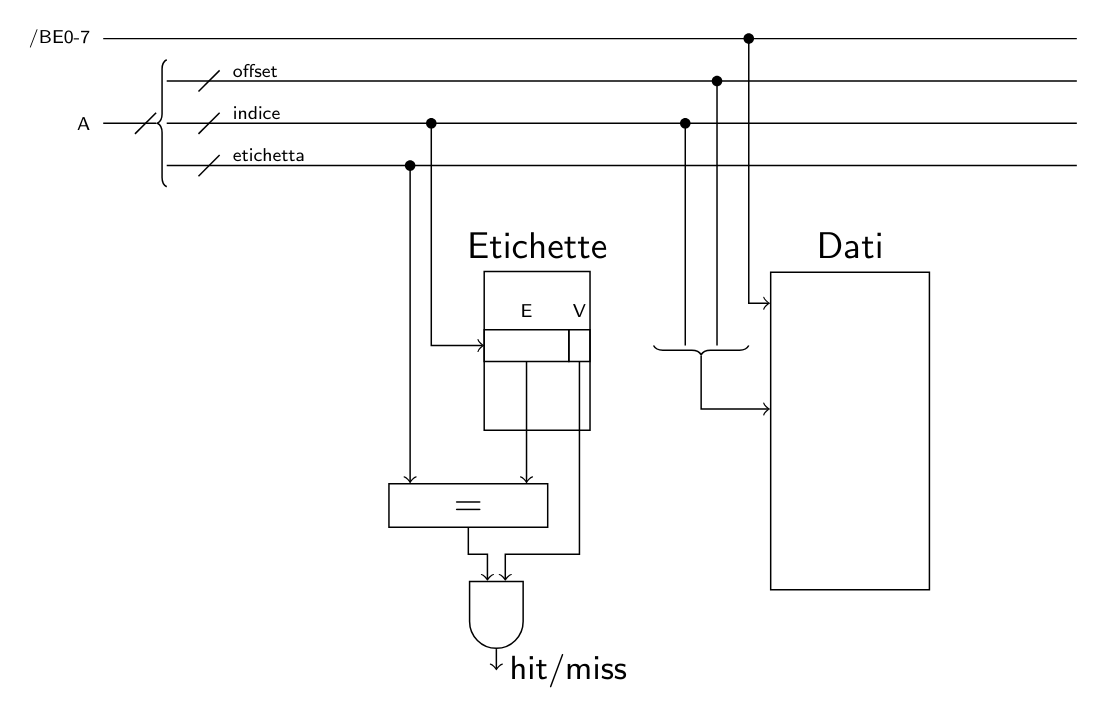
\includegraphics[scale = 0.5]{../figures/cache_diretta.png}
\end{center}
\end{minipage}

\subsubsection{Lettura}
A questo punto, in fase di lettura, nel caso di hit basterà ricavare una linea di offset dai bit meno significativi di A, e leggere dalla memoria cache a tale offset, all'indice indicato dall'etichetta.
Nel caso di miss si dovrà invece svolgere la lettura in memoria RAM, e poi riportare l'informazione nella cacheline di indice giusto della cache aggiornando l'etichetta.

\subsubsection{Scrittura}
Per quanto riguarda le scritture invece, potremo muoverci in due strade: \textbf{write allocate} e \textbf{write no allocate}.

\begin{itemize}
	\item \textbf{Write allocate:}
ci comportiamo in maniera simile alla lettura nel caso di hit.
Nel caso di miss, invece, riportiamo il dato in cache.

A questo punto potremmo pensare di svolgere la scrittura in RAM e in cache contemporaneamente (regola \textit{write-through}), mantenendo entrambe aggiornate.

Una tecnica più intelligente può invece essere quella di aggiornare il solo dato in cache, e rimandare la scrittura in RAM alla rimozione del dato dalla cache (per l'introduzione di un nuovo dato allo stesso indice) (regola \textit{write-back}).
In questo caso dovremo dotarci di un nuovo bit nella memoria delle etichette, il bit \textit{dirty}, che segnalerà il bisogno di ricopiare il dato in cache nella RAM in occasione del suo deallocamento dalla cache.
La difficoltà principale di questo metodo è l'avere un agente che non è la CPU che scrive in RAM, e come vedremo richiede soluzioni tecniche particolari.

\item \textbf{Write no allocate:}
in questo caso ignoriamo le scritture in cache e la sfruttiamo solamente per le letture.

\end{itemize}

\par\smallskip

Notiamo che questa cache soffre di problemi di \textbf{collisione}: infatti ci sarà un numero di regioni con lo stesso indice ed etichetta diversa, pari alla dimensione della RAM fratto la dimensione della cache.

\end{document}


\documentclass[a4paper,11pt]{article}
\usepackage[a4paper, margin=8em]{geometry}

% usa i pacchetti per la scrittura in italiano
\usepackage[french,italian]{babel}
\usepackage[T1]{fontenc}
\usepackage[utf8]{inputenc}
\frenchspacing 

% usa i pacchetti per la formattazione matematica
\usepackage{amsmath, amssymb, amsthm, amsfonts}

% usa altri pacchetti
\usepackage{gensymb}
\usepackage{hyperref}
\usepackage{standalone}

\usepackage{colortbl}

\usepackage{xstring}
\usepackage{karnaugh-map}

% imposta il titolo
\title{Appunti Calcolatori Elettronici}
\author{Luca Seggiani}
\date{2025}

% imposta lo stile
% usa helvetica
\usepackage[scaled]{helvet}
% usa palatino
\usepackage{palatino}
% usa un font monospazio guardabile
\usepackage{lmodern}

\renewcommand{\rmdefault}{ppl}
\renewcommand{\sfdefault}{phv}
\renewcommand{\ttdefault}{lmtt}

% circuiti
\usepackage{circuitikz}
\usetikzlibrary{babel}

% testo cerchiato
\newcommand*\circled[1]{\tikz[baseline=(char.base)]{
            \node[shape=circle,draw,inner sep=2pt] (char) {#1};}}

% disponi il titolo
\makeatletter
\renewcommand{\maketitle} {
	\begin{center} 
		\begin{minipage}[t]{.8\textwidth}
			\textsf{\huge\bfseries \@title} 
		\end{minipage}%
		\begin{minipage}[t]{.2\textwidth}
			\raggedleft \vspace{-1.65em}
			\textsf{\small \@author} \vfill
			\textsf{\small \@date}
		\end{minipage}
		\par
	\end{center}

	\thispagestyle{empty}
	\pagestyle{fancy}
}
\makeatother

% disponi teoremi
\usepackage{tcolorbox}
\newtcolorbox[auto counter, number within=section]{theorem}[2][]{%
	colback=blue!10, 
	colframe=blue!40!black, 
	sharp corners=northwest,
	fonttitle=\sffamily\bfseries, 
	title=Teorema~\thetcbcounter: #2, 
	#1
}

% disponi definizioni
\newtcolorbox[auto counter, number within=section]{definition}[2][]{%
	colback=red!10,
	colframe=red!40!black,
	sharp corners=northwest,
	fonttitle=\sffamily\bfseries,
	title=Definizione~\thetcbcounter: #2,
	#1
}

% disponi codice
\usepackage{listings}
\usepackage[table]{xcolor}

\definecolor{codegreen}{rgb}{0,0.6,0}
\definecolor{codegray}{rgb}{0.5,0.5,0.5}
\definecolor{codepurple}{rgb}{0.58,0,0.82}
\definecolor{backcolour}{rgb}{0.95,0.95,0.92}

\lstdefinestyle{codestyle}{
		backgroundcolor=\color{black!5}, 
		commentstyle=\color{codegreen},
		keywordstyle=\bfseries\color{magenta},
		numberstyle=\sffamily\tiny\color{black!60},
		stringstyle=\color{green!50!black},
		basicstyle=\ttfamily\footnotesize,
		breakatwhitespace=false,         
		breaklines=true,                 
		captionpos=b,                    
		keepspaces=true,                 
		numbers=left,                    
		numbersep=5pt,                  
		showspaces=false,                
		showstringspaces=false,
		showtabs=false,                  
		tabsize=2
}

\lstdefinestyle{shellstyle}{
		backgroundcolor=\color{black!5}, 
		basicstyle=\ttfamily\footnotesize\color{black}, 
		commentstyle=\color{black}, 
		keywordstyle=\color{black},
		numberstyle=\color{black!5},
		stringstyle=\color{black}, 
		showspaces=false,
		showstringspaces=false, 
		showtabs=false, 
		tabsize=2, 
		numbers=none, 
		breaklines=true
}


\lstdefinelanguage{assembler}{ 
  keywords={AAA, AAD, AAM, AAS, ADC, ADCB, ADCW, ADCL, ADD, ADDB, ADDW, ADDL, AND, ANDB, ANDW, ANDL,
        ARPL, BOUND, BSF, BSFL, BSFW, BSR, BSRL, BSRW, BSWAP, BT, BTC, BTCB, BTCW, BTCL, BTR, 
        BTRB, BTRW, BTRL, BTS, BTSB, BTSW, BTSL, CALL, CBW, CDQ, CLC, CLD, CLI, CLTS, CMC, CMP,
        CMPB, CMPW, CMPL, CMPS, CMPSB, CMPSD, CMPSW, CMPXCHG, CMPXCHGB, CMPXCHGW, CMPXCHGL,
        CMPXCHG8B, CPUID, CWDE, DAA, DAS, DEC, DECB, DECW, DECL, DIV, DIVB, DIVW, DIVL, ENTER,
        HLT, IDIV, IDIVB, IDIVW, IDIVL, IMUL, IMULB, IMULW, IMULL, IN, INB, INW, INL, INC, INCB,
        INCW, INCL, INS, INSB, INSD, INSW, INT, INT3, INTO, INVD, INVLPG, IRET, IRETD, JA, JAE,
        JB, JBE, JC, JCXZ, JE, JECXZ, JG, JGE, JL, JLE, JMP, JNA, JNAE, JNB, JNBE, JNC, JNE, JNG,
        JNGE, JNL, JNLE, JNO, JNP, JNS, JNZ, JO, JP, JPE, JPO, JS, JZ, LAHF, LAR, LCALL, LDS,
        LEA, LEAVE, LES, LFS, LGDT, LGS, LIDT, LMSW, LOCK, LODSB, LODSD, LODSW, LOOP, LOOPE,
        LOOPNE, LSL, LSS, LTR, MOV, MOVB, MOVW, MOVL, MOVSB, MOVSD, MOVSW, MOVSX, MOVSXB,
        MOVSXW, MOVSXL, MOVZX, MOVZXB, MOVZXW, MOVZXL, MUL, MULB, MULW, MULL, NEG, NEGB, NEGW,
        NEGL, NOP, NOT, NOTB, NOTW, NOTL, OR, ORB, ORW, ORL, OUT, OUTB, OUTW, OUTL, OUTSB, OUTSD,
        OUTSW, POP, POPL, POPW, POPB, POPA, POPAD, POPF, POPFD, PUSH, PUSHL, PUSHW, PUSHB, PUSHA, 
				PUSHAD, PUSHF, PUSHFD, RCL, RCLB, RCLW, MOVSL, MOVSB, MOVSW, STOSL, STOSB, STOSW, LODSB, LODSW,
				LODSL, INSB, INSW, INSL, OUTSB, OUTSL, OUTSW
        RCLL, RCR, RCRB, RCRW, RCRL, RDMSR, RDPMC, RDTSC, REP, REPE, REPNE, RET, ROL, ROLB, ROLW,
        ROLL, ROR, RORB, RORW, RORL, SAHF, SAL, SALB, SALW, SALL, SAR, SARB, SARW, SARL, SBB,
        SBBB, SBBW, SBBL, SCASB, SCASD, SCASW, SETA, SETAE, SETB, SETBE, SETC, SETE, SETG, SETGE,
        SETL, SETLE, SETNA, SETNAE, SETNB, SETNBE, SETNC, SETNE, SETNG, SETNGE, SETNL, SETNLE,
        SETNO, SETNP, SETNS, SETNZ, SETO, SETP, SETPE, SETPO, SETS, SETZ, SGDT, SHL, SHLB, SHLW,
        SHLL, SHLD, SHR, SHRB, SHRW, SHRL, SHRD, SIDT, SLDT, SMSW, STC, STD, STI, STOSB, STOSD,
        STOSW, STR, SUB, SUBB, SUBW, SUBL, TEST, TESTB, TESTW, TESTL, VERR, VERW, WAIT, WBINVD,
        XADD, XADDB, XADDW, XADDL, XCHG, XCHGB, XCHGW, XCHGL, XLAT, XLATB, XOR, XORB, XORW, XORL},
  keywordstyle=\color{blue}\bfseries,
  ndkeywordstyle=\color{darkgray}\bfseries,
  identifierstyle=\color{black},
  sensitive=false,
  comment=[l]{\#},
  morecomment=[s]{/*}{*/},
  commentstyle=\color{purple}\ttfamily,
  stringstyle=\color{red}\ttfamily,
  morestring=[b]',
  morestring=[b]"
}

\lstset{language=assembler, style=codestyle}

% disponi sezioni
\usepackage{titlesec}

\titleformat{\section}
	{\sffamily\Large\bfseries} 
	{\thesection}{1em}{} 
\titleformat{\subsection}
	{\sffamily\large\bfseries}   
	{\thesubsection}{1em}{} 
\titleformat{\subsubsection}
	{\sffamily\normalsize\bfseries} 
	{\thesubsubsection}{1em}{}

% tikz
\usepackage{tikz}

% float
\usepackage{float}

% grafici
\usepackage{pgfplots}
\pgfplotsset{width=10cm,compat=1.9}

% disponi alberi
\usepackage{forest}

\forestset{
	rectstyle/.style={
		for tree={rectangle,draw,font=\large\sffamily}
	},
	roundstyle/.style={
		for tree={circle,draw,font=\large}
	}
}

% disponi algoritmi
\usepackage{algorithm}
\usepackage{algorithmic}
\makeatletter
\renewcommand{\ALG@name}{Algoritmo}
\makeatother

% disponi numeri di pagina
\usepackage{fancyhdr}
\fancyhf{} 
\fancyfoot[L]{\sffamily{\thepage}}

\makeatletter
\fancyhead[L]{\raisebox{1ex}[0pt][0pt]{\sffamily{\@title \ \@date}}} 
\fancyhead[R]{\raisebox{1ex}[0pt][0pt]{\sffamily{\@author}}}
\makeatother

\begin{document}
% sezione (data)
\section{Lezione del 07-03-25}

% stili pagina
\thispagestyle{empty}
\pagestyle{fancy}

% testo
Riprendiamo il discorso della memoria cache.
Avevamo che questa è montata fra la CPU e lo spazio di memoria.
Più propriamente, questa si trova fra la CPU e il bus.

In questo, può vedere non solo le operazioni sulla memoria, ma anche sullo spazio di I/O.
In questo caso, però, dovrà ovviamente comportarsi sempre in maniera \textit{read-through} e \textit{write-through}, quindi effettivamente disattivarsi e lasciare che il processore interagisca direttamente con l'I/O.

Questo è dovuto al fatto che allo spazio di I/O potrebbero accedere e modificare dati dispositivi esterni alla CPU (le interfacce), operazione che invaliderebbe immediatamente qualsiasi cosa venga scritta in memoriaa cache.

Inoltre, ogni operazione di lettura può comportare di per sé un aggiornamento delle interfacce, che comporterà un aggiornamento della memoria, motivo per cui un operazione di caching sarebbe superflua.

Operazione simile varrà effettuata per la memoria video (che non sta nello spazio di I/O).
Questa facoltà verra realizzata dalla cache attraverso, probabilmente, \textit{maschere} o \textit{tabelle}.

\subsubsection{Cache associative ad insiemi}
Avevamo visto come il difetto principale della cache ad indirizzamento diretta è quello delle \textit{collisioni}.
Presentiamo un metodo, quello delle \textbf{cache associative ad insiemi}, che risolve il problema permettendo di allocare più cacheline allo stesso indirizzo.

Duplichiamo quindi la struttura vista per la cache ad indirizzamento diretto (qui 2 volte), e sruttiamo le uscite hit/miss delle singole memorie delle etichette per pilotare un multiplexer con in ingresso le linee dati delle memorie di cache corrispondenti.

In questo caso a letture allo stesso indice le cache potranno rispondere diversamente (magari la prima in miss e la seconda in hit), e il processore vedrà ritornarsi il dato corretto (in questo caso quello della seconda).

Compito di scegliere quale cache sfruttare nel caso di collisioni è quello del \textbf{controllore} di cache (nella cache ad indirizzamento diretto non c'era scelta). 
La scelta migliore possibile sarebbe quella di scegliere la cacheline al cui i accederà più tardi nel futuro (per mantenere i dati immediatamente utili nella cache).

Chiaramente, visto che non si può prevedere il futuro (o almeno non lo possono fare né la CPU né il controllore di cache), occorre adottare un euristica.
Una di queste euristiche è la politica \textbf{LRU} (\textit{Least Recently Used}), dove si sceglie la cacheline al quale non si accede da più tempo.

Per realizzare tale politica si sfrutta una memoria, che chiamiamo $R$.
Con solo due vie, basterà memorizzare su $R$ l'ultima via usata, e quella su cui scriviere sarà immediatamente l'altra.

Con più di due vie sarebbe necessario mantenere l'ordine degli accessi, cio per $n$ vie ricordare informazione necessaria a controllare $n!$ diverse possibilità.
Nella pratica, però, conviene usare politiche approssimate.

\subsubsection{Pseudo-LRU dell'80486}
Vediamo una di queste politiche approssimate, che gestiva 4 vie attraverso 3 bit $b_00$, $b_1$ e $b_2$.
Si usava un albero binario per la selezione di una delle vie, disposto come:
\begin{center}
	\begin{forest}
		[$b_0$, roundstyle
			[$b_1$
				[A, rectstyle]
				[B, rectstyle]
				]
			[$b_2$
				[C, rectstyle]
				[D, rectstyle]
			]
		]	
	\end{forest}
\end{center}
dove i valori 1 sono i rami a destra, e viceversa i valori 0 sono i rami a sinistra.

In fase di rimpiazzamento, si sceglie la via seguendo l'albero.
In fase di accesso, si modificano i $b_i$ in modo da portare la via a cui si è fasso accesso in fondo all'ordinamento che si ottiene visitando l'albero.
L'errore può essere dato dal fatto che la via che si trova nello stesso gruppo della via a cui si è fatto accesso potrebbe trovarsi ad un indice più alto del necessario, visto che si abbassa cumulativamente l'intero gruppo aggiornando $b_0$.

\par\smallskip

Per cache più grandi si sfruttano sempre algoritmi ad albero di questo tipo, magari tagliando i rami più bassi per lasciare spazio a scelte completamente casuali.

Notiamo poi che le memorie cache di questo tipo incontrano sempre difficoltà quando si fanno accessi ciclici ad indici che si ripetono con un modulo con il numero di vie diverso da zero: ad esempio se si leggono ciclicamente 5 indirizzi che corrispondono allo stesso indice, la cache non riuscirà mai a mantenere tutti e 5 in una delle cacheline delle vie, e quindi ogni accesso comporterà un miss.

\subsubsection{Livelli di cache}
Nei processori moderni si hanno solitamente più livelli di cache (3 o 4), che crescono in dimensioni e associatività più si vanno a disporre "lontano" dal processore e "vicini" alla RAM.
Le cache di livello più basso saranno quindi più veloci ma più piccole, mentre le cache di livelo alto saranno più lente ma più grandi.

Il controllore di cache provvederà a gestire i livelli di cache, effettuando gli accessi controllando a partire dal livello più basso (più veloce) per arrivare al livello più basso, fino alla RAM.

\subsection{Interruzioni}
La limitazione principale del processore studiato finora è che il flusso di controllo è completamente determinato dal programma in esecuzione.
Attraverso il meccanismo dell'interruzione, il sistema definisce $e_1, ..., e_n$ \textbf{eventi}, e il programmatore $r_1, ..., r_n$ \textbf{routine} per la gestione di tali eventi.
Da qui in poi il processore continua ad eseguire il suo normale flusso di controllo, ma monitorando in qualche modo lo stato di questi eventi.
Nel caso uno degli eventi $e_i$ effettivamente si verifichi, la CPU provvederà a sospendere il flusso di controllo attuale e ad eseguire la routine $r_i$.

Un esempio classico dell'utilità di un meccanismo di questo tipo è dato dalle fasi di stampa che avevamo definito per dispositivi come le stampanti: attraverso l'approcio visto finora dovremmo controllare periodicamente un certo registro di stato per verificare la possibilità di scrivere un nuovo dato in un certo registro di buffer.
Questo occupa la CPU con operazioni inutili, che potrebbe saltare se fosse la stampante stessa ad avvertirla di quando è pronta a ricevere un nuovo dato.

L'idea di base è quella di avere una nuova operazione da svolgere in fase di esecuzione di un instruzione da parte della CPU, dopo l'esecuzione dell'istruzione stessa.
Ad esempio, potremmo riportarci un bit di valdiità, \lstinline|READY|, da parte della stampante, e controllarlo ad ogni istruzione per la chiamata di una routine di stampa.
La chiamata sarà semplicemente un aggiornamento condizionato a RIP, con scrittura del contenuto attuale di RIP in pila (che è compatibile con le regole di chiamata dei sottoprogrammi a cui siamo abituati).

Un problema di questo approccio potrebbe essere che, se il bit che segnala l'evento non si aggiorna immediatamente, la CPU andrà in un ciclo continuo di arresto dell'esecuzione e inizio di una routine.
Una soluzione potrebbe essere dotare della CPU di una \textit{rete di accettazione} della richiesta: il bit di segnalazione dell'evento va in un generatore di impulsi che setta un SR flip-flop. 
A questo punto la CPU risponde (livello hardware, nella nuova fase di esecuzione appena descritta) con un segnale di reset nel momento in cui riesce a rilevare l'evento e spostarsi nella routine. 

In verità la situazione è più complicata: ad esempio potremmo voler ignorare nuovi eventi quando stiamo già cercando di soddisfarne uno.
Per questo i processori x86 prevedono un apposito flag, il flag \textbf{IF} (\textit{Interruption Flag}), che determina se le nuove interruzioni dovranno essere soddisfatte o meno.
Il processore può essere quindi configurato per attivare automaticamente il flag IF in fase di risposta ad una richiesta di interruzione.
Per effettuare il corretto ritorno, si usa la funzione \lstinline|IRETQ|, che ripristina, oltre ad altre cose, lo stato dei flag (che era stato salvato in pila).



\end{document}


\documentclass[a4paper,11pt]{article}
\usepackage[a4paper, margin=8em]{geometry}

% usa i pacchetti per la scrittura in italiano
\usepackage[french,italian]{babel}
\usepackage[T1]{fontenc}
\usepackage[utf8]{inputenc}
\frenchspacing 

% usa i pacchetti per la formattazione matematica
\usepackage{amsmath, amssymb, amsthm, amsfonts}

% usa altri pacchetti
\usepackage{gensymb}
\usepackage{hyperref}
\usepackage{standalone}

\usepackage{colortbl}

\usepackage{xstring}
\usepackage{karnaugh-map}

% imposta il titolo
\title{Appunti Calcolatori Elettronici}
\author{Luca Seggiani}
\date{2025}

% imposta lo stile
% usa helvetica
\usepackage[scaled]{helvet}
% usa palatino
\usepackage{palatino}
% usa un font monospazio guardabile
\usepackage{lmodern}

\renewcommand{\rmdefault}{ppl}
\renewcommand{\sfdefault}{phv}
\renewcommand{\ttdefault}{lmtt}

% circuiti
\usepackage{circuitikz}
\usetikzlibrary{babel}

% testo cerchiato
\newcommand*\circled[1]{\tikz[baseline=(char.base)]{
            \node[shape=circle,draw,inner sep=2pt] (char) {#1};}}

% disponi il titolo
\makeatletter
\renewcommand{\maketitle} {
	\begin{center} 
		\begin{minipage}[t]{.8\textwidth}
			\textsf{\huge\bfseries \@title} 
		\end{minipage}%
		\begin{minipage}[t]{.2\textwidth}
			\raggedleft \vspace{-1.65em}
			\textsf{\small \@author} \vfill
			\textsf{\small \@date}
		\end{minipage}
		\par
	\end{center}

	\thispagestyle{empty}
	\pagestyle{fancy}
}
\makeatother

% disponi teoremi
\usepackage{tcolorbox}
\newtcolorbox[auto counter, number within=section]{theorem}[2][]{%
	colback=blue!10, 
	colframe=blue!40!black, 
	sharp corners=northwest,
	fonttitle=\sffamily\bfseries, 
	title=Teorema~\thetcbcounter: #2, 
	#1
}

% disponi definizioni
\newtcolorbox[auto counter, number within=section]{definition}[2][]{%
	colback=red!10,
	colframe=red!40!black,
	sharp corners=northwest,
	fonttitle=\sffamily\bfseries,
	title=Definizione~\thetcbcounter: #2,
	#1
}

% disponi codice
\usepackage{listings}
\usepackage[table]{xcolor}

\definecolor{codegreen}{rgb}{0,0.6,0}
\definecolor{codegray}{rgb}{0.5,0.5,0.5}
\definecolor{codepurple}{rgb}{0.58,0,0.82}
\definecolor{backcolour}{rgb}{0.95,0.95,0.92}

\lstdefinestyle{codestyle}{
		backgroundcolor=\color{black!5}, 
		commentstyle=\color{codegreen},
		keywordstyle=\bfseries\color{magenta},
		numberstyle=\sffamily\tiny\color{black!60},
		stringstyle=\color{green!50!black},
		basicstyle=\ttfamily\footnotesize,
		breakatwhitespace=false,         
		breaklines=true,                 
		captionpos=b,                    
		keepspaces=true,                 
		numbers=left,                    
		numbersep=5pt,                  
		showspaces=false,                
		showstringspaces=false,
		showtabs=false,                  
		tabsize=2
}

\lstdefinestyle{shellstyle}{
		backgroundcolor=\color{black!5}, 
		basicstyle=\ttfamily\footnotesize\color{black}, 
		commentstyle=\color{black}, 
		keywordstyle=\color{black},
		numberstyle=\color{black!5},
		stringstyle=\color{black}, 
		showspaces=false,
		showstringspaces=false, 
		showtabs=false, 
		tabsize=2, 
		numbers=none, 
		breaklines=true
}


\lstdefinelanguage{assembler}{ 
  keywords={AAA, AAD, AAM, AAS, ADC, ADCB, ADCW, ADCL, ADD, ADDB, ADDW, ADDL, AND, ANDB, ANDW, ANDL,
        ARPL, BOUND, BSF, BSFL, BSFW, BSR, BSRL, BSRW, BSWAP, BT, BTC, BTCB, BTCW, BTCL, BTR, 
        BTRB, BTRW, BTRL, BTS, BTSB, BTSW, BTSL, CALL, CBW, CDQ, CLC, CLD, CLI, CLTS, CMC, CMP,
        CMPB, CMPW, CMPL, CMPS, CMPSB, CMPSD, CMPSW, CMPXCHG, CMPXCHGB, CMPXCHGW, CMPXCHGL,
        CMPXCHG8B, CPUID, CWDE, DAA, DAS, DEC, DECB, DECW, DECL, DIV, DIVB, DIVW, DIVL, ENTER,
        HLT, IDIV, IDIVB, IDIVW, IDIVL, IMUL, IMULB, IMULW, IMULL, IN, INB, INW, INL, INC, INCB,
        INCW, INCL, INS, INSB, INSD, INSW, INT, INT3, INTO, INVD, INVLPG, IRET, IRETD, JA, JAE,
        JB, JBE, JC, JCXZ, JE, JECXZ, JG, JGE, JL, JLE, JMP, JNA, JNAE, JNB, JNBE, JNC, JNE, JNG,
        JNGE, JNL, JNLE, JNO, JNP, JNS, JNZ, JO, JP, JPE, JPO, JS, JZ, LAHF, LAR, LCALL, LDS,
        LEA, LEAVE, LES, LFS, LGDT, LGS, LIDT, LMSW, LOCK, LODSB, LODSD, LODSW, LOOP, LOOPE,
        LOOPNE, LSL, LSS, LTR, MOV, MOVB, MOVW, MOVL, MOVSB, MOVSD, MOVSW, MOVSX, MOVSXB,
        MOVSXW, MOVSXL, MOVZX, MOVZXB, MOVZXW, MOVZXL, MUL, MULB, MULW, MULL, NEG, NEGB, NEGW,
        NEGL, NOP, NOT, NOTB, NOTW, NOTL, OR, ORB, ORW, ORL, OUT, OUTB, OUTW, OUTL, OUTSB, OUTSD,
        OUTSW, POP, POPL, POPW, POPB, POPA, POPAD, POPF, POPFD, PUSH, PUSHL, PUSHW, PUSHB, PUSHA, 
				PUSHAD, PUSHF, PUSHFD, RCL, RCLB, RCLW, MOVSL, MOVSB, MOVSW, STOSL, STOSB, STOSW, LODSB, LODSW,
				LODSL, INSB, INSW, INSL, OUTSB, OUTSL, OUTSW
        RCLL, RCR, RCRB, RCRW, RCRL, RDMSR, RDPMC, RDTSC, REP, REPE, REPNE, RET, ROL, ROLB, ROLW,
        ROLL, ROR, RORB, RORW, RORL, SAHF, SAL, SALB, SALW, SALL, SAR, SARB, SARW, SARL, SBB,
        SBBB, SBBW, SBBL, SCASB, SCASD, SCASW, SETA, SETAE, SETB, SETBE, SETC, SETE, SETG, SETGE,
        SETL, SETLE, SETNA, SETNAE, SETNB, SETNBE, SETNC, SETNE, SETNG, SETNGE, SETNL, SETNLE,
        SETNO, SETNP, SETNS, SETNZ, SETO, SETP, SETPE, SETPO, SETS, SETZ, SGDT, SHL, SHLB, SHLW,
        SHLL, SHLD, SHR, SHRB, SHRW, SHRL, SHRD, SIDT, SLDT, SMSW, STC, STD, STI, STOSB, STOSD,
        STOSW, STR, SUB, SUBB, SUBW, SUBL, TEST, TESTB, TESTW, TESTL, VERR, VERW, WAIT, WBINVD,
        XADD, XADDB, XADDW, XADDL, XCHG, XCHGB, XCHGW, XCHGL, XLAT, XLATB, XOR, XORB, XORW, XORL},
  keywordstyle=\color{blue}\bfseries,
  ndkeywordstyle=\color{darkgray}\bfseries,
  identifierstyle=\color{black},
  sensitive=false,
  comment=[l]{\#},
  morecomment=[s]{/*}{*/},
  commentstyle=\color{purple}\ttfamily,
  stringstyle=\color{red}\ttfamily,
  morestring=[b]',
  morestring=[b]"
}

\lstset{language=assembler, style=codestyle}

% disponi sezioni
\usepackage{titlesec}

\titleformat{\section}
	{\sffamily\Large\bfseries} 
	{\thesection}{1em}{} 
\titleformat{\subsection}
	{\sffamily\large\bfseries}   
	{\thesubsection}{1em}{} 
\titleformat{\subsubsection}
	{\sffamily\normalsize\bfseries} 
	{\thesubsubsection}{1em}{}

% tikz
\usepackage{tikz}

% float
\usepackage{float}

% grafici
\usepackage{pgfplots}
\pgfplotsset{width=10cm,compat=1.9}

% disponi alberi
\usepackage{forest}

\forestset{
	rectstyle/.style={
		for tree={rectangle,draw,font=\large\sffamily}
	},
	roundstyle/.style={
		for tree={circle,draw,font=\large}
	}
}

% disponi algoritmi
\usepackage{algorithm}
\usepackage{algorithmic}
\makeatletter
\renewcommand{\ALG@name}{Algoritmo}
\makeatother

% disponi numeri di pagina
\usepackage{fancyhdr}
\fancyhf{} 
\fancyfoot[L]{\sffamily{\thepage}}

\makeatletter
\fancyhead[L]{\raisebox{1ex}[0pt][0pt]{\sffamily{\@title \ \@date}}} 
\fancyhead[R]{\raisebox{1ex}[0pt][0pt]{\sffamily{\@author}}}
\makeatother

\begin{document}
% sezione (data)
\section{Lezione del 10-03-25}

% stili pagina
\thispagestyle{empty}
\pagestyle{fancy}

% testo
Torniamo sull'argomento delle interruzioni, specificando il modo in cui dobbiamo definire dei \textit{gestori} per ogni interruzione.

Il calcolatore visto finora dispone di 4 interfacce: \begin{itemize}
	\item L'interfaccia \textit{tastiera}, letta finora in controllo di programma, valutando la validità di un bit FI sul registro di stato;
	\item L'interfaccia \textit{timer}, dotata di 3 singoli timer, di cui abbiamo detto il primo viene usato per generare interruzioni, il secondo non è più usato, e il terzo e connesso al \textit{beeper speaker};
	\item L'interfaccia a blocchi per \textit{hard disk}, che accede ad un drive pilotando in base al suo stato un registro di stato (per noi era utile implementare la funzione di attesa del drive a controllo programma \lstinline|wait_for_br()|).
\end{itemize} 

Ignoriamo, per adesso, il video.
Ognuna di queste interfacce può trarre beneficio dalla presenza di interruzioni:
\begin{itemize}
	\item La tastiera potrebbe \textit{avvertirci} dei nuovi tasti premuti, anziché costringerci a controllare;
	\item Il timer ci deve avvisare, al termine del conteggio del timer 0, attraverso un interruzione;
	\item L'hard disk, come la tastiera, ci può avvisare con un interruzione quando è pronto ad una nuova scrittura.
\end{itemize}

Questo comportamento, delle cosiddette \textbf{interruzioni esterne}, è definito nella macchina studiata dal \textbf{controllore delle interruzioni}, che è l'Intel \textbf{APIC} (\textit{Advanced Progammable Interruption Controller}).
Questo scansiona periodicamente tutte le linee di richiesta d'interruzione (le \textbf{IRQ}) ottenute dalle varie interfacce, e invia le interruzioni corrispondenti, una per volta, alla CPU. 

Avevamo già reputato necessario specificare un \textbf{tipo di interruzione}, su 8 bit (per 256 tipi) per ogni interruzione lanciata.
L'APIC, allora, fornirà semplicemente la possibilità di assegnare un tipo di interruzione diverso ad ogni piedino di ingresso dall interfacce, in modo che si possa assegnare ad ogni interruzione la routine di gestione più adatta.
In questo, la configurazione dell'APIC si svolge come la configurazione di una qualsiasi periferica attraverso un'apposita interfaccia.

La comunicazione fra CPU e APIC in fase di interruzione viene effettuata attraverso un \textit{handshake} su due linee, \textbf{INTR} (\textit{Interrupt Request}) e \textbf{INTA} (\textit{Interrupt Acknowledge}), che comporta anche una lettura da parte della CPU di quanto l'APIC metterà sul bus (cioè il tipo di interruzione).

A questo punto, le routine vere e proprie verrano definite nell'\textbf{IDT}, (\textit{Interrupt Descriptor Table}), contenente in sequenza gli indirizzi delle prime istruzioni di ogni routine per ogni tipo di interruzione, e specificata a partire da un certo indirizzo indicato nel registro \textbf{IDTR}.

Come abbiamo visto, la reazione o meno della CPU ad una interuzione è data dall'attivazione del flag IF.
Nel caso si passi effettivamente ad eseguire l'interruzione, ricordiamo che sia l'IP che lo stato dei flags verrà salvato in pila, e ripristinato a fine routine attraverso l'istruzione \lstinline|IRET|.

\subsubsection{Rilevamento di interruzioni da parte dell'APIC}
Potremmo chiederci come fa il controllore APIC a capire quando un'interfaccia sta richiedendo una nuova richiesta.

Un primo approccio potrebbe essere di non rileggere il piedino di ingresso di quell'interfaccia, all'ottenimento e successivo invio alla CPU di un interruzione, fino alla segnalazione, sempre da parte della CPU, di avvenuta gestione dell'interruzione.
Questo può essere effettuato dotando l'APIC di un opportuno registro (\textbf{EOI}, \textit{End Of Interrupt}), che la CPU andrà a modificare conclusa la gestione dell'interruzione.

Un approccio più sicuro può essere ottenuto dotando il controllore delle interruzioni di due registri, entrambi su 256 bit (un bit per ogni tipo di interruzione):
\begin{itemize}
	\item \textbf{IRR} (\textit{Interrupt Request Register}): indica con bit alti quali interruzioni sono state inviate dalle interfacce attualmente;
	\item \textbf{ISR} (\textit{Interrupt Service Register}): indica con bit alti a quali interruzioni sta rispondendo il processore attualmente. In un processore single-threaded come quello che studiamo al più uno solo dei suoi bit sarà alto in un dato momento (escluso il caso della \textit{gestione annidata}).
\end{itemize}

Si avrà quindi la seguente organizzazione:
\begin{table}[h!]
	\center 
	\begin{tabular} { c | c  }
		\textbf{IRR}, \textit{Interrupt Request Register} & 256 bit \\
		\textbf{ISR}, \textit{Interrupt Service Register} & 256 bit
	\end{tabular}
\end{table}

Un interruzione generata lato hardware si tradurrà nell'innalzamento (se non era già alto) di un bit nell'IRR, e l'inizio (o schedulazione dell'inizio) di un handshake con la CPU.
Al termine dell'handshake (quindi all'abbassamento di INTA successivo ad un suo innalzamento per acknowledge) il bit dell'interruzione corrente passa dall'IRR all'ISR.
Infine, la transizione dal bit presente nell'ISR all'interruzione gestita (bit nuovamente basso) si ha sempre con il segnale EOI da parte della CPU (con successivo inizio, se necessario, di un nuovo ciclo di handshake per una nuova richiesta di interruzione).

\subsubsection{Priorità delle interruzioni e gestione annidata}
Ci rendiamo quindi conto che alcune richieste sono più importanti di altre: ad esempio, la pressione di un tasto su tastiera può essere ignorata, se ad esempio nel frattempo arriva una richiesta di interruzione da parte di un timer.
La pressione del tasto non si ripeterà infatti in tempo utile, mentre il timer potrebbe inviarci nuove richieste mentre ancora non siamo pronti a riceverle, e continuerà a farlo a scadenze regolari (potremmo finire per gestire solo un sottoinsieme delle richieste che ci vengono effettivamente inviate).

Possiamo quindi chiederci come l'APIC si comporta in caso di più richieste concorrenti.
Un idea potrebbe essere di assegnare una priorità ad ogni richiesta, e rispondere prima alle richieste di priorità più alta.
Questa priorità può essere implementata chiamando i 4 bit più significativi del tipo dell'interruzione \textbf{classe di precedenza} dell'interruzione: a classi di precedenza maggiore abbiamo gestione prioritaria delle richieste di interruzione.
Il trasferimento da IRR a ISR avverrà quindi prima per richieste di classe di precedenza più alta, e poi per quelle di classe di precedenza \textit{uguale} o più bassa, con la possibilità per le prime di \textit{interrompere} i gestori di interruzione delle ultime.

La precedenza delle interruzioni è quindi necessaria all'implementazione corretta della \textbf{gestione annidata} delle interruzioni, dove un interruzione di precedenza più altra può interrompere (a patto che IF sia alto) un gestore di interruzione in esecuzione. 
Questo è il caso a cui accennavamo prima, dove più bit di ISR possono essere alti contemporaneamente (a patto che si dispongano nel tempo, da destra verso sinistra, cioè da minore priorità a maggiore priorità), e che si risolvano da sinistra verso destra (cioè da maggiore priorità a minore priorità).

\end{document}


\documentclass[a4paper,11pt]{article}
\usepackage[a4paper, margin=8em]{geometry}

% usa i pacchetti per la scrittura in italiano
\usepackage[french,italian]{babel}
\usepackage[T1]{fontenc}
\usepackage[utf8]{inputenc}
\frenchspacing 

% usa i pacchetti per la formattazione matematica
\usepackage{amsmath, amssymb, amsthm, amsfonts}

% usa altri pacchetti
\usepackage{gensymb}
\usepackage{hyperref}
\usepackage{standalone}

\usepackage{colortbl}

\usepackage{xstring}
\usepackage{karnaugh-map}

% imposta il titolo
\title{Appunti Calcolatori Elettronici}
\author{Luca Seggiani}
\date{2025}

% imposta lo stile
% usa helvetica
\usepackage[scaled]{helvet}
% usa palatino
\usepackage{palatino}
% usa un font monospazio guardabile
\usepackage{lmodern}

\renewcommand{\rmdefault}{ppl}
\renewcommand{\sfdefault}{phv}
\renewcommand{\ttdefault}{lmtt}

% circuiti
\usepackage{circuitikz}
\usetikzlibrary{babel}

% testo cerchiato
\newcommand*\circled[1]{\tikz[baseline=(char.base)]{
\node[shape=circle,draw,inner sep=2pt] (char) {#1};}}

% disponi il titolo
\makeatletter
\renewcommand{\maketitle} {
	\begin{center} 
		\begin{minipage}[t]{.8\textwidth}
			\textsf{\huge\bfseries \@title} 
		\end{minipage}%
		\begin{minipage}[t]{.2\textwidth}
			\raggedleft \vspace{-1.65em}
			\textsf{\small \@author} \vfill
			\textsf{\small \@date}
		\end{minipage}
		\par
	\end{center}

	\thispagestyle{empty}
	\pagestyle{fancy}
}
\makeatother

% disponi teoremi
\usepackage{tcolorbox}
\newtcolorbox[auto counter, number within=section]{theorem}[2][]{%
	colback=blue!10, 
	colframe=blue!40!black, 
	sharp corners=northwest,
	fonttitle=\sffamily\bfseries, 
	title=Teorema~\thetcbcounter: #2, 
	#1
}

% disponi definizioni
\newtcolorbox[auto counter, number within=section]{definition}[2][]{%
	colback=red!10,
	colframe=red!40!black,
	sharp corners=northwest,
	fonttitle=\sffamily\bfseries,
	title=Definizione~\thetcbcounter: #2,
	#1
}

% disponi codice
\usepackage{listings}
\usepackage[table]{xcolor}

\definecolor{codegreen}{rgb}{0,0.6,0}
\definecolor{codegray}{rgb}{0.5,0.5,0.5}
\definecolor{codepurple}{rgb}{0.58,0,0.82}
\definecolor{backcolour}{rgb}{0.95,0.95,0.92}

\lstdefinestyle{codestyle}{
	backgroundcolor=\color{black!5}, 
	commentstyle=\color{codegreen},
	keywordstyle=\bfseries\color{magenta},
	numberstyle=\sffamily\tiny\color{black!60},
	stringstyle=\color{green!50!black},
	basicstyle=\ttfamily\footnotesize,
	breakatwhitespace=false,         
	breaklines=true,                 
	captionpos=b,                    
	keepspaces=true,                 
	numbers=left,                    
	numbersep=5pt,                  
	showspaces=false,                
	showstringspaces=false,
	showtabs=false,                  
	tabsize=2
}

\lstdefinestyle{shellstyle}{
	backgroundcolor=\color{black!5}, 
	basicstyle=\ttfamily\footnotesize\color{black}, 
	commentstyle=\color{black}, 
	keywordstyle=\color{black},
	numberstyle=\color{black!5},
	stringstyle=\color{black}, 
	showspaces=false,
	showstringspaces=false, 
	showtabs=false, 
	tabsize=2, 
	numbers=none, 
	breaklines=true
}


\lstdefinelanguage{assembler}{ 
	keywords={AAA, AAD, AAM, AAS, ADC, ADCB, ADCW, ADCL, ADD, ADDB, ADDW, ADDL, AND, ANDB, ANDW, ANDL,
		ARPL, BOUND, BSF, BSFL, BSFW, BSR, BSRL, BSRW, BSWAP, BT, BTC, BTCB, BTCW, BTCL, BTR, 
		BTRB, BTRW, BTRL, BTS, BTSB, BTSW, BTSL, CALL, CBW, CDQ, CLC, CLD, CLI, CLTS, CMC, CMP,
		CMPB, CMPW, CMPL, CMPS, CMPSB, CMPSD, CMPSW, CMPXCHG, CMPXCHGB, CMPXCHGW, CMPXCHGL,
		CMPXCHG8B, CPUID, CWDE, DAA, DAS, DEC, DECB, DECW, DECL, DIV, DIVB, DIVW, DIVL, ENTER,
		HLT, IDIV, IDIVB, IDIVW, IDIVL, IMUL, IMULB, IMULW, IMULL, IN, INB, INW, INL, INC, INCB,
		INCW, INCL, INS, INSB, INSD, INSW, INT, INT3, INTO, INVD, INVLPG, IRET, IRETD, JA, JAE,
		JB, JBE, JC, JCXZ, JE, JECXZ, JG, JGE, JL, JLE, JMP, JNA, JNAE, JNB, JNBE, JNC, JNE, JNG,
		JNGE, JNL, JNLE, JNO, JNP, JNS, JNZ, JO, JP, JPE, JPO, JS, JZ, LAHF, LAR, LCALL, LDS,
		LEA, LEAVE, LES, LFS, LGDT, LGS, LIDT, LMSW, LOCK, LODSB, LODSD, LODSW, LOOP, LOOPE,
		LOOPNE, LSL, LSS, LTR, MOV, MOVB, MOVW, MOVL, MOVSB, MOVSD, MOVSW, MOVSX, MOVSXB,
		MOVSXW, MOVSXL, MOVZX, MOVZXB, MOVZXW, MOVZXL, MUL, MULB, MULW, MULL, NEG, NEGB, NEGW,
		NEGL, NOP, NOT, NOTB, NOTW, NOTL, OR, ORB, ORW, ORL, OUT, OUTB, OUTW, OUTL, OUTSB, OUTSD,
		OUTSW, POP, POPL, POPW, POPB, POPA, POPAD, POPF, POPFD, PUSH, PUSHL, PUSHW, PUSHB, PUSHA, 
		PUSHAD, PUSHF, PUSHFD, RCL, RCLB, RCLW, MOVSL, MOVSB, MOVSW, STOSL, STOSB, STOSW, LODSB, LODSW,
		LODSL, INSB, INSW, INSL, OUTSB, OUTSL, OUTSW
		RCLL, RCR, RCRB, RCRW, RCRL, RDMSR, RDPMC, RDTSC, REP, REPE, REPNE, RET, ROL, ROLB, ROLW,
		ROLL, ROR, RORB, RORW, RORL, SAHF, SAL, SALB, SALW, SALL, SAR, SARB, SARW, SARL, SBB,
		SBBB, SBBW, SBBL, SCASB, SCASD, SCASW, SETA, SETAE, SETB, SETBE, SETC, SETE, SETG, SETGE,
		SETL, SETLE, SETNA, SETNAE, SETNB, SETNBE, SETNC, SETNE, SETNG, SETNGE, SETNL, SETNLE,
		SETNO, SETNP, SETNS, SETNZ, SETO, SETP, SETPE, SETPO, SETS, SETZ, SGDT, SHL, SHLB, SHLW,
		SHLL, SHLD, SHR, SHRB, SHRW, SHRL, SHRD, SIDT, SLDT, SMSW, STC, STD, STI, STOSB, STOSD,
		STOSW, STR, SUB, SUBB, SUBW, SUBL, TEST, TESTB, TESTW, TESTL, VERR, VERW, WAIT, WBINVD,
	XADD, XADDB, XADDW, XADDL, XCHG, XCHGB, XCHGW, XCHGL, XLAT, XLATB, XOR, XORB, XORW, XORL},
	keywordstyle=\color{blue}\bfseries,
	ndkeywordstyle=\color{darkgray}\bfseries,
	identifierstyle=\color{black},
	sensitive=false,
	comment=[l]{\#},
	morecomment=[s]{/*}{*/},
	commentstyle=\color{purple}\ttfamily,
	stringstyle=\color{red}\ttfamily,
	morestring=[b]',
	morestring=[b]"
}

\lstset{language=assembler, style=codestyle}

% disponi sezioni
\usepackage{titlesec}

\titleformat{\section}
{\sffamily\Large\bfseries} 
{\thesection}{1em}{} 
\titleformat{\subsection}
{\sffamily\large\bfseries}   
{\thesubsection}{1em}{} 
\titleformat{\subsubsection}
{\sffamily\normalsize\bfseries} 
{\thesubsubsection}{1em}{}

% tikz
\usepackage{tikz}

% float
\usepackage{float}

% grafici
\usepackage{pgfplots}
\pgfplotsset{width=10cm,compat=1.9}

% disponi alberi
\usepackage{forest}

\forestset{
	rectstyle/.style={
		for tree={rectangle,draw,font=\large\sffamily}
	},
	roundstyle/.style={
		for tree={circle,draw,font=\large}
	}
}

% disponi algoritmi
\usepackage{algorithm}
\usepackage{algorithmic}
\makeatletter
\renewcommand{\ALG@name}{Algoritmo}
\makeatother

% disponi numeri di pagina
\usepackage{fancyhdr}
\fancyhf{} 
\fancyfoot[L]{\sffamily{\thepage}}

\makeatletter
\fancyhead[L]{\raisebox{1ex}[0pt][0pt]{\sffamily{\@title \ \@date}}} 
\fancyhead[R]{\raisebox{1ex}[0pt][0pt]{\sffamily{\@author}}}
\makeatother

\begin{document}
% sezione (data)
\section{Lezione del 11-03-25}

% stili pagina
\thispagestyle{empty}
\pagestyle{fancy}

% testo
Riprendiamo la trattazione dell controllore di interruzini APIC.

\subsubsection{Interruzione di livello o di fronte}
Vediamo un dettaglio sul comportamento dell'APIC: questo può rilevare, in base alla sua configurazione, i \textbf{livelli} o i \textbf{fronti} delle variabili in ingresso.

Questo può avere delle implicazioni diverse a seconda dell'interfaccia.
Ad esempio, avevamo detto che il timer in modalità 2 genera un onda quadra.
Se si usa una routine lanciata dal timer a interruzione di programma, e si configura l'APIC per rilevare il livello, potrebbe essere che a routine concluse il livello del timer è sempre alto, e quindi l'interruzione viene lanciata nuovamente.

Questo è chiaramente diverso dal comportamento desiderato, ed è quindi opportuno configurare l'APIC per rilevare i soli fronti di salita.

\par\medskip

Abbiamo quindi notato praticamente tutte le caratteristiche che ci interessavano dell'APIC, e possiamo procedere ad implementare un esempio di gestione di un interfaccia a controllo di interruzione.
Vediamo ad esempio il seguente programma, che gestisce la tastiera a controllo di interruzione, di cui la parte C++:
\lstset{style=codestyle, language=C++}
\lstinputlisting{../code/interrupts/hw_basic/main.cpp}
e la parte assembly:
\lstset{style=codestyle, language=assembler}
\lstinputlisting{../code/interrupts/hw_basic/main.s}

Il meccanismo di chiamata dell'interruzione (macro per il salvataggio/caricamento registri, istruzione \lstinline|iretq|, ecc...) è identico all'esempio precedente.
Una novità è la presenza della funzione \lstinline|send_EOI()| nel gestore di interruzione, che invia il segnale di End Of Interrupt all'APIC e gli fa capire, assieme alla lettura che facciamo sulla tastiera (con \lstinline|kbd::get_code()|) che l'interruzione è stata effettivamente gestita.
Inoltre, la parte di configurazione dell'interruzione è più complessa.
Bisogna infatti:
\begin{itemize}
	\item Attivare le interruzioni da tastiera con \lstinline|kbd::enable_intr()|;
	\item Impostare l'APIC per inviare tali interruzini al tipo interruzione \lstinline|0x20|, configurandolo per riconoscere fronti, e disattivando la maschera (rispettivamente \lstinline|set_TRGM()| e \lstinline|set_MIRQ|);
	\item Infine, inizializzare il gate corrispondente al tipo interruzione \lstinline|0x20| come avevamo già visto.
\end{itemize}

Abbiamo quindi realizzato pienamente quanto ci eravamo posti di fare quando abbiamo iniziato a parlare di interruzione: la CPU è lasciata libera (nell'esempio specifico, esegue un loop infinito), e viene \textit{interrotta} dalla periferica tastiera quando questa ha un nuovo dato disponibile.
Vediamo che in verità esiste un altra casistica di applicazione delle interruzioni che non abbiamo trattato, cioè quella delle \textit{eccezioni}.

\subsection{Eccezioni}
Ci rimangono da vedere le \textbf{eccezioni}.
Queste sono particolari errori logici che il processore potrebbe incontrare nel corso dell'esecuzione, come ad esempio la divisione per 0, il tentativo di eseguire un istruzione non riconosciuta, ecc...

Una differenza fra le interruzioni esterne e le eccezioni è che le eccezioni possono essere sollevate \textit{durante} la lettura e esecuzione di un istruzione, quindi ad esempio mentre si stava interpetando un codice operativo (si pensi all'interruzione di operazione non riconosciuta).
In verità, per assicurare l'atomicità dei cicli di esecuzione, la CPU ripristina automaticamente il suo stato a prima del lancio dell'interruzione.
In particolare, possiamo distinguere 3 tipi di eccezione:
\begin{itemize}
	\item \textbf{Fault:} l'esecuzione non viene ancora eseguita, lo stato IP prima della sua esecuzione viene salvato (quindi si rimane alla stessa istruzione), e si può riprovare ad eseguirla dopo aver risolto l'errore;
	\item \textbf{Trap:} l'esecuzione ormai è stata eseguita, e si salva l'IP successivo.
	\item \textbf{Abort:} raggruppa degli eventi particolarmente disastrosi in cui l'esecuzione si arresta completamente (ad esempio la tripla eccezione).
\end{itemize}

Quando viene lanciata una \textit{fault} o una \textit{trap}, il processore cerca nella IDT se esiste un handler corrispondente (segnalato attraverso un bit nell'IDT stessa, alla riga della tabella corrispondente all'eccezione considerata).
Nel caso questo non esista, si riprova con la fault di \textit{doppia eccezione}, che quindi rappresenta una fault a sé.
Nel caso nemmeno questo handler esista, viene lanciata una fault di \textit{tripla eccezione}, che è di tipo \textit{abort} e comporta quindi l'arresto del programma.

\par\medskip

Vediamo quindi un programma di esempio delle eccezioni, che gestisce ad esempio la divisione per zero (tipo \lstinline|0x00| nella IDT), di cui la parte C++:
\lstset{style=codestyle, language=C++}
\lstinputlisting{../code/interrupts/div_zero/main.cpp}
e la parte assembly:
\lstset{style=codestyle, language=assembler}
\lstinputlisting{../code/interrupts/div_zero/main.s}

Notiamo che questo è il primo esempio che vediamo di valore di ritorno dal gestore di eccezione: il valore di RIP al momento dell'interruzione, che viene passato nel registro \lstinline|%RDI| (come definisce l'ABI System V).

\subsubsection{Eccezioni e debug}
Un interruzione particolare è quella rappresentata da \lstinline|INT3|, l'interruzione di \textit{debug}.
Attraverso questa, un \textit{debugger} è capace di interrompere l'esecuzione di un programma ad un certo indirizzo del suo codice macchina.

Un'altra interruzione di debug è data dalla single step, che viene lanciata ad ogni istruzione quando è attivo un certo flag (appunto, il flag single step). Questo permette al debugger di eseguire il programma in modalità \textit{passo singolo}, cioè eseguendo un istruzione e interrompendo, permettendo al programmatore di osservare il suo andamento passo per passo.

\subsection{Riassunto sui tipi di interruzioni}
Abbiamo quindi visto tutti i tipi di interruzione, di cui riportiamo una lista completa:
\begin{itemize}
	\item \textbf{Interruzioni esterne:} causate da interfacce esterne e gestite dall'APIC I/O, di cui distinguiamo:
		\begin{itemize}
			\item \textbf{Interruzioni esterne mascherabli:} quelle che abbiamo visto finora, relative a normali eventi I/O;
			\item \textbf{Interruzioni esterne non mascherabili:} cioè che non possono essere mascherate, solitamente rappresentano eventi particolarmente gravi o comunque la cui gestione ha alta importanza.
		\end{itemize}
	\item \textbf{Interruzioni interne} (\textit{Eccezioni}): eventi che non arrivano dall'esterno, ma si generano all'interno del processore stesso;
	\item \textbf{Interruzioni software:} interruzioni che vengono lanciate direttamente dal programma attraverso l'istruzione \lstinline|INT|, la cui utilità è stata per ora dimostrativa, e verrà inquadrata meglio studiando il meccanismo della \textit{protezione}, e in generale lo sviluppo del sistema multiprogrammato e delle relative \textit{primitive}.
\end{itemize}

\end{document}


\documentclass[a4paper,11pt]{article}
\usepackage[a4paper, margin=8em]{geometry}

% usa i pacchetti per la scrittura in italiano
\usepackage[french,italian]{babel}
\usepackage[T1]{fontenc}
\usepackage[utf8]{inputenc}
\frenchspacing 

% usa i pacchetti per la formattazione matematica
\usepackage{amsmath, amssymb, amsthm, amsfonts}

% usa altri pacchetti
\usepackage{gensymb}
\usepackage{hyperref}
\usepackage{standalone}

\usepackage{colortbl}

\usepackage{xstring}
\usepackage{karnaugh-map}

% imposta il titolo
\title{Appunti Calcolatori Elettronici}
\author{Luca Seggiani}
\date{2025}

% imposta lo stile
% usa helvetica
\usepackage[scaled]{helvet}
% usa palatino
\usepackage{palatino}
% usa un font monospazio guardabile
\usepackage{lmodern}

\renewcommand{\rmdefault}{ppl}
\renewcommand{\sfdefault}{phv}
\renewcommand{\ttdefault}{lmtt}

% circuiti
\usepackage{circuitikz}
\usetikzlibrary{babel}

% testo cerchiato
\newcommand*\circled[1]{\tikz[baseline=(char.base)]{
            \node[shape=circle,draw,inner sep=2pt] (char) {#1};}}

% disponi il titolo
\makeatletter
\renewcommand{\maketitle} {
	\begin{center} 
		\begin{minipage}[t]{.8\textwidth}
			\textsf{\huge\bfseries \@title} 
		\end{minipage}%
		\begin{minipage}[t]{.2\textwidth}
			\raggedleft \vspace{-1.65em}
			\textsf{\small \@author} \vfill
			\textsf{\small \@date}
		\end{minipage}
		\par
	\end{center}

	\thispagestyle{empty}
	\pagestyle{fancy}
}
\makeatother

% disponi teoremi
\usepackage{tcolorbox}
\newtcolorbox[auto counter, number within=section]{theorem}[2][]{%
	colback=blue!10, 
	colframe=blue!40!black, 
	sharp corners=northwest,
	fonttitle=\sffamily\bfseries, 
	title=Teorema~\thetcbcounter: #2, 
	#1
}

% disponi definizioni
\newtcolorbox[auto counter, number within=section]{definition}[2][]{%
	colback=red!10,
	colframe=red!40!black,
	sharp corners=northwest,
	fonttitle=\sffamily\bfseries,
	title=Definizione~\thetcbcounter: #2,
	#1
}

% disponi codice
\usepackage{listings}
\usepackage[table]{xcolor}

\definecolor{codegreen}{rgb}{0,0.6,0}
\definecolor{codegray}{rgb}{0.5,0.5,0.5}
\definecolor{codepurple}{rgb}{0.58,0,0.82}
\definecolor{backcolour}{rgb}{0.95,0.95,0.92}

\lstdefinestyle{codestyle}{
		backgroundcolor=\color{black!5}, 
		commentstyle=\color{codegreen},
		keywordstyle=\bfseries\color{magenta},
		numberstyle=\sffamily\tiny\color{black!60},
		stringstyle=\color{green!50!black},
		basicstyle=\ttfamily\footnotesize,
		breakatwhitespace=false,         
		breaklines=true,                 
		captionpos=b,                    
		keepspaces=true,                 
		numbers=left,                    
		numbersep=5pt,                  
		showspaces=false,                
		showstringspaces=false,
		showtabs=false,                  
		tabsize=2
}

\lstdefinestyle{shellstyle}{
		backgroundcolor=\color{black!5}, 
		basicstyle=\ttfamily\footnotesize\color{black}, 
		commentstyle=\color{black}, 
		keywordstyle=\color{black},
		numberstyle=\color{black!5},
		stringstyle=\color{black}, 
		showspaces=false,
		showstringspaces=false, 
		showtabs=false, 
		tabsize=2, 
		numbers=none, 
		breaklines=true
}


\lstdefinelanguage{assembler}{ 
  keywords={AAA, AAD, AAM, AAS, ADC, ADCB, ADCW, ADCL, ADD, ADDB, ADDW, ADDL, AND, ANDB, ANDW, ANDL,
        ARPL, BOUND, BSF, BSFL, BSFW, BSR, BSRL, BSRW, BSWAP, BT, BTC, BTCB, BTCW, BTCL, BTR, 
        BTRB, BTRW, BTRL, BTS, BTSB, BTSW, BTSL, CALL, CBW, CDQ, CLC, CLD, CLI, CLTS, CMC, CMP,
        CMPB, CMPW, CMPL, CMPS, CMPSB, CMPSD, CMPSW, CMPXCHG, CMPXCHGB, CMPXCHGW, CMPXCHGL,
        CMPXCHG8B, CPUID, CWDE, DAA, DAS, DEC, DECB, DECW, DECL, DIV, DIVB, DIVW, DIVL, ENTER,
        HLT, IDIV, IDIVB, IDIVW, IDIVL, IMUL, IMULB, IMULW, IMULL, IN, INB, INW, INL, INC, INCB,
        INCW, INCL, INS, INSB, INSD, INSW, INT, INT3, INTO, INVD, INVLPG, IRET, IRETD, JA, JAE,
        JB, JBE, JC, JCXZ, JE, JECXZ, JG, JGE, JL, JLE, JMP, JNA, JNAE, JNB, JNBE, JNC, JNE, JNG,
        JNGE, JNL, JNLE, JNO, JNP, JNS, JNZ, JO, JP, JPE, JPO, JS, JZ, LAHF, LAR, LCALL, LDS,
        LEA, LEAVE, LES, LFS, LGDT, LGS, LIDT, LMSW, LOCK, LODSB, LODSD, LODSW, LOOP, LOOPE,
        LOOPNE, LSL, LSS, LTR, MOV, MOVB, MOVW, MOVL, MOVSB, MOVSD, MOVSW, MOVSX, MOVSXB,
        MOVSXW, MOVSXL, MOVZX, MOVZXB, MOVZXW, MOVZXL, MUL, MULB, MULW, MULL, NEG, NEGB, NEGW,
        NEGL, NOP, NOT, NOTB, NOTW, NOTL, OR, ORB, ORW, ORL, OUT, OUTB, OUTW, OUTL, OUTSB, OUTSD,
        OUTSW, POP, POPL, POPW, POPB, POPA, POPAD, POPF, POPFD, PUSH, PUSHL, PUSHW, PUSHB, PUSHA, 
				PUSHAD, PUSHF, PUSHFD, RCL, RCLB, RCLW, MOVSL, MOVSB, MOVSW, STOSL, STOSB, STOSW, LODSB, LODSW,
				LODSL, INSB, INSW, INSL, OUTSB, OUTSL, OUTSW
        RCLL, RCR, RCRB, RCRW, RCRL, RDMSR, RDPMC, RDTSC, REP, REPE, REPNE, RET, ROL, ROLB, ROLW,
        ROLL, ROR, RORB, RORW, RORL, SAHF, SAL, SALB, SALW, SALL, SAR, SARB, SARW, SARL, SBB,
        SBBB, SBBW, SBBL, SCASB, SCASD, SCASW, SETA, SETAE, SETB, SETBE, SETC, SETE, SETG, SETGE,
        SETL, SETLE, SETNA, SETNAE, SETNB, SETNBE, SETNC, SETNE, SETNG, SETNGE, SETNL, SETNLE,
        SETNO, SETNP, SETNS, SETNZ, SETO, SETP, SETPE, SETPO, SETS, SETZ, SGDT, SHL, SHLB, SHLW,
        SHLL, SHLD, SHR, SHRB, SHRW, SHRL, SHRD, SIDT, SLDT, SMSW, STC, STD, STI, STOSB, STOSD,
        STOSW, STR, SUB, SUBB, SUBW, SUBL, TEST, TESTB, TESTW, TESTL, VERR, VERW, WAIT, WBINVD,
        XADD, XADDB, XADDW, XADDL, XCHG, XCHGB, XCHGW, XCHGL, XLAT, XLATB, XOR, XORB, XORW, XORL},
  keywordstyle=\color{blue}\bfseries,
  ndkeywordstyle=\color{darkgray}\bfseries,
  identifierstyle=\color{black},
  sensitive=false,
  comment=[l]{\#},
  morecomment=[s]{/*}{*/},
  commentstyle=\color{purple}\ttfamily,
  stringstyle=\color{red}\ttfamily,
  morestring=[b]',
  morestring=[b]"
}

\lstset{language=assembler, style=codestyle}

% disponi sezioni
\usepackage{titlesec}

\titleformat{\section}
	{\sffamily\Large\bfseries} 
	{\thesection}{1em}{} 
\titleformat{\subsection}
	{\sffamily\large\bfseries}   
	{\thesubsection}{1em}{} 
\titleformat{\subsubsection}
	{\sffamily\normalsize\bfseries} 
	{\thesubsubsection}{1em}{}

% tikz
\usepackage{tikz}

% float
\usepackage{float}

% grafici
\usepackage{pgfplots}
\pgfplotsset{width=10cm,compat=1.9}

% disponi alberi
\usepackage{forest}

\forestset{
	rectstyle/.style={
		for tree={rectangle,draw,font=\large\sffamily}
	},
	roundstyle/.style={
		for tree={circle,draw,font=\large}
	}
}

% disponi algoritmi
\usepackage{algorithm}
\usepackage{algorithmic}
\makeatletter
\renewcommand{\ALG@name}{Algoritmo}
\makeatother

% disponi numeri di pagina
\usepackage{fancyhdr}
\fancyhf{} 
\fancyfoot[L]{\sffamily{\thepage}}

\makeatletter
\fancyhead[L]{\raisebox{1ex}[0pt][0pt]{\sffamily{\@title \ \@date}}} 
\fancyhead[R]{\raisebox{1ex}[0pt][0pt]{\sffamily{\@author}}}
\makeatother

\begin{document}
% sezione (data)
\section{Lezione del 17-03-25}

% stili pagina
\thispagestyle{empty}
\pagestyle{fancy}

% testo
\subsection{Protezione}
Tutti i programmi che abbiamo visto finora hanno il pieno controllo su la macchina su cui sono in esecuzione.
Questo significa che possono impattare qualsiasi regione di memoria, incluso il loro stesso codice macchina, o i frame di stack di programmi lanciati prima di loro.

Un approccio di questo tipo non è ideale quando più programmi, magari di utenti diversi, vengono lanciati ed eseguiti \textit{quasi} in contemporanea (\textit{time-sharing}) sulla stessa macchina.

Un esempio di questa situazione può verificarsi nel caso di esecuziono \textit{batch}, cioè di esecuzione successiva di più programmi, magari scritti da più utenti.
Vorremmo massimizzare l'uso della CPU sospendendo un programma e iniziandone un altro nel caso il primo fra questi inizi un'operazione che richiede una quantità significativa di tempo (ad esempio un accesso a un dispositivo di I/O).
In questo caso, visto che non possiamo fidarci della benevolenza degli utenti nell'inserire istruzioni esplicite per il cambio da un programma all'altro, vorremo agire sull'hardware per, ad esempio, vietare all'utente l'uso di certe istruzioni (qui \lstinline|IN| e \lstinline|OUT|) e costringerlo ad usare primitive messe a disposizione dal sistema.

Chiaramente, però, le primitive dovranno poter usare \lstinline|IN| e \lstinline|OUT| per fare l'I/O vero e proprio con i dispositivi.
Per permettere questo doppio comportamento introduciamo l'idea di \textbf{protezione}.

\subsubsection{Contesti di esecuzione}
Il programma nella memoria potrà essere in esecuzione, in un momento qualsiasi, in uno di due \textbf{contesti}, o \textit{modi} (vedremo nell'architettura x86 corrente, si parla di protezione a \textit{ring}): il contesto \textbf{sistema} e il contesto \textbf{utente}.
Le istruzioni di cui permetterà l'esecuzione saranno quindi determinate dal contesto corrente.

Forniamo allora il processore di un apposito registro, il \textbf{CS} (\textit{Code Segment}), a 2 bit.
I 2 bit sono necessari in quanto storicamente (il meccanismo descritto viene introdotto nell'architettura x86 a partire dal 286) si definivano quattro contesti, o \textbf{ring}:
\begin{table}[h!]
	\center \rowcolors{2}{white}{black!10}
	\begin{tabular} { c | c | c }
		\bfseries CS & \bfseries Ring & \bfseries Tipo \\
		\hline 
		00 & Ring 0 & Kernel (sistema) \\
		01 & Ring 1 & Driver \\
		10 & Ring 2 &  / / \\
		11 & Ring 3 & Utente \\
	\end{tabular}
\end{table}

Il nome CS deriva dal fatto che questo registro era pensato per gestire la \textit{segmentazione} della memoria.
Sia questo meccanismo, che i due ring interni (l'1 e il 2) sono pressoché inutilizzati nell'architettura x86-64 moderna, e quindi li ignoreremo, portandoci effettivamente alla situazione dove CS rappresenta un flag che distingue fra contesto \textit{sistema} e contesto \textit{utente}, come avevamo ipotizzato.

\subsubsection{Transizioni fra contesti}
Ipotizziamo quindi che all'avvio si parta in contesto sistema, e che si passi al contesto utente quando si esegue un programma utente, 
Per permettere all'utente di "accedere" alle istruzioni privilegiate, vogliamo che questo disponga di un modo di tornare al contesto sistema, ma lasciando il controllo al sistema operativo (altrimenti sarebbe inutile introdurre l'idea di un contesto utente in primo luogo).
Di contro, vogliamo un modo per il sistema operativo di restituire in sicurezza il controllo al programma, previa transizione del processore in contesto utente.

Vediamo come il meccanismo dell'interruzione fornisce un metodo per gestire questa situazione.

Introdurremo un tipo di interruzione apposito, che restituisce il controllo al sistema operativo (semplicemente passando ad un gestore di interruzione definito dal sistema operativo) passando a contesto sistema.
Il tipo di operazione che stiamo richedendo al sistema operativo potrà essere passato in qualche registro specifico, solitamente \lstinline|%EAX|.
Il problema potrebbe essere chiaramente che l'utente ha la possibilità di modificare tutta la memoria, e quindi la stessa IDT e il gestore impostato.

\subsubsection{Protezione di memoria}
Si rende quindi necessario un meccanismo di gestione degli accessi in memoria.
In contesto utente, quindi, oltre a permettere l'utilizzo di solo alcune istruzioni \textit{non privilegiate}, il processore dovrà permettere l'accesso solo a determinate regioni di memoria. 
Visto che non abbiamo ancora introdotto l'idea di \textit{memoria virtuale}, modellizziamo temporaneamente questa configurazione con un apposito registro a controllo sistema che decide quali regioni di memoria sono o non sono accessibili.

Abbiamo quindi l'immagine completa del meccanismo della protezione, che avevamo introdotto per privilegiare le sole istruzioni, ma ci rendiamo adesso conto deve consistere in:
\begin{itemize}
	\item Protezione delle \textbf{istruzioni} attraverso il loro privilegiamento al contesto sistema, come avevamo visto;
	\item Protezione della \textbf{memoria} definendo regioni accessibili in sola modalità sistema.
\end{itemize}

\subsubsection{Transizione da contesto utente a contesto sistema}
Vediamo nel dettaglio come si passa dal contesto utente al contesto sistema.
Per questo sfrutteremo l'istruzione x86 \lstinline|INT|, che permette di generare un interruzione software sulla base del tipo fornito come operando.
Si potrà quindi implementare il meccanismo della \textit{chiamata a sistemo}, secondo una modalità del tipo:
\begin{lstlisting}[language=assembler, style=codestyle]	
mov $0x00, %eax # tipo chiamata
int $0x80       # chiamata sistema (per x86, in x96-64 esiste syscall)
\end{lstlisting}
Notiamo che questo è l'approccio normalmente supportato dai moderni sistemi operativi x86 (specialmente Linux, anche se oggi si usa l'istruzione apposita \lstinline|syscall|).
Vedremo che il passaggio del tipo chiamata nel registro \lstinline|%EAX| non si verifica nel kernel che studieremo, dove invece ognuno dei 224 tipi di interruzioni liberi potrà rappresentare una chiamata a sistema diversa.

Questo si tradurrà a livello processore nel salvataggio dello stato corrente di esecuzione, la transizione al contesto sistema e lo spostamento in IP della prima istruzione di un apposito sottoprograma di servizio atto a gestire l'eccezione (e quindi soddisfare, se possibile, la richiesta del programma per cui questo ha sollevato in primo luogo l'interruzione).

Per capire nel dettaglio cosa accade nel processore è necessario:
\begin{itemize}
	\item Capire come è strutturata la Interrupt Descriptor Table (IDT) all'interno della memoria del sistema, che supponiamo essere privilegiata (altrimenti l'utente potrebbe manometterla);
	\item Capire come viene gestita un interruzione software, cioè come si conserva lo stato al momento dell'interruzione, e come si inizia l'esecuzione del gestore in contesto sistema.
\end{itemize}

Vediamo questi dettagli in ordine.

\subsubsection{Struttura della IDT}
Vediamo quindi nel dettaglio la struttura di un entrata della IDT.
Questa viene a trovarsi nella memoria privilegiata a partire da un indirizzo, come avevamo detto, contenuto nel registro IDTR.
L'impostazione di questo registro si fa attraverso apposite istruzioni, sempre ad accesso privilegiato.

Le entrate dell'IDT si chiamano \textbf{gate IDT}, che si distinguono in 3 tipi, \textit{Task Gate}, \textit{Interrupt Gate} e \textit{Trap Gate}, che al momento non vediamo.
La struttura a livello di memoria contiene le seguenti informazioni:
\begin{itemize}
	\item L'offset della routine di gestione dell'interruzione, in alcune modalità comprendente dell'indice di segmento, ecc...;
	\item \textbf{P:} un flag di \textbf{presenza}, indica se il descrittore è effettivamente abilitato;
	\item \textbf{L:} il livello di protezione (contesto sistema o utente) a cui deve essere eseguito il gestore. Notiamo che questa sembra essere una semplificazione del corso (il professore si è rivelato ombroso a riguardo). In verità, l'IDT mantiene un riferimento al CS dell'istruzione, che anche se ora abbiamo assunto come un semplice flag sistema/utente, rappresenta invece un riferimento al \textit{segmento} vero e proprio all'interno del cui è allocata la routine. Informazioni riguardo al livello di ring di ogni segmento sono contenute in altre tabelle specifiche, dette \textbf{GDT} (\textit{Global Descriptor Table}) e \textbf{LDT} (\textit{Local Descriptor Table}). Il salto al livello L viene quindi fatto automaticamente in base al livello del segmento in cui è allocato il gestore (vediamo che con considerazioni simili si capisce come mai viene allocato, oltre a RIP, anche il CS corrente in fase di chiamata);
	\item \textbf{I/T:} il tipo di interruzione fra quelli sopra definiti.
	\item \textbf{DPL:} il livello minimo da cui si può accedere al gestore come interruzione interna (attraverso una \lstinline|INT|).
		Questo non significa che tale gestore non possa essere lanciato da un eccezione. 
\end{itemize}		

Sorvolando su alcuni dettagli non immediatamente rilevanti (il valore del \textit{Segment Selector} SS è piuttosto complesso, ma è quello che va a definire quello che noi intediamo con L), la struttura generale di un'entrata dell'IDT è quindi la seguente:
\begin{center}
	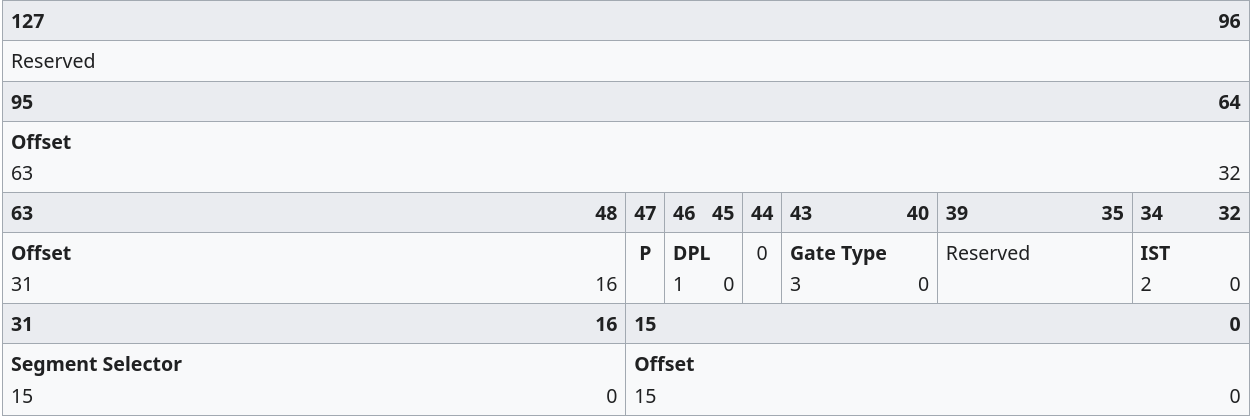
\includegraphics[scale=0.45]{../figures/entrata_idt.png}
\end{center}
come riportato su \url{https://wiki.osdev.org/Interrupt_Descriptor_Table}.

\subsubsection{Gestione dell'interruzione software}
Avevamo visto come il meccanismo dell'interruzione, definito un gate nella IDT, si riduceva al caricamento in RIP dell'indirizzo del gestore e dell'immissione in pila dei seguenti dati:
\begin{table}[H]
	\center
	\begin{tabular} { c | p{5cm} }
		\lstinline|0| & RIP \\
		\lstinline|+1| & CS \\
		\lstinline|+2| & RFLAGS 
	\end{tabular}
\end{table}
Cioè si impostava un nuovo frame sulla pila con i seguenti dati:
\begin{itemize}
	\item L'instruction pointer \textbf{RIP}, da dove si vorrà ripartire nell'esecuzione una volta gestita l'interruzione.
		Notiamo che in verità questo indirizzo, che è fra l'altro in memoria virtuale, è corredato a seconda del tipo di gate dall'\textbf{SS} (\textit{Stack Segment}) o dal \textbf{TSS} (\textit{Task State Segment}), utili alla memoria segmentata che come abbiamo visto non ci è di interesse. La caratteristica importante è che si conserva un riferimento a dove ripartire, in memoria, nell'esecuzione una volta gestita l'interruzione;
	\item Il contenuto attuale di \textbf{CS}, cioè il contesto al momento della chiamata, che chiaramente vorremo ristabilire in seguito;
	\item Come abbiamo visto, anche \textbf{RFLAGS} viene memorizzato, in quanto gli interrupt mascherabili vengono mascherati in fase di gestione di un interrupt sistema (attraverso il flag \textbf{IF}), e vogliamo resettare questo comportamente al termine della gestione.
\end{itemize}

A questo punto l'unica differenza nella chiamata di interrupt in caso di cambio di contesto sta effettivamente nella transizione fra due \textbf{pile}: la separazione fra contesto utente e contesto sistema viene infatti resa possibile anche dalla presenza di due pile separate, di cui l'ultima chiaramente sta in memoria protetta.
Il programma è normalmente in esecuzione nella pila utente: al momento del sollevamento di un interruzione software, si passa all'esecuzione (se alcune condizioni che vedremo fra poco sono rispettate) della routine di gestione definita dal sistema operativo.
Questo richiede un modo per preservare la posizione della pila utente, da cui ci spostiamo quando passiamo alla pila sistema.
Facciamo ciò conservando il vecchio \textbf{RSP}, immettendolo in pila prima dei registri visti prima, cioè creando un frame del tipo:
\begin{table}[H]
	\center
	\begin{tabular} { c | p{7cm} }
		\lstinline|0| & RIP \\
		\lstinline|+1| & CS \\
		\lstinline|+2| & RFLAGS \\ 
		\lstinline|+3| & RSP (Pila utente)
	\end{tabular}
\end{table}
Il vecchio valore di RSP permetterà, fra l'altro, di accedere e modificare il contesto del \textit{processo} in esecuzione con la sua pila utente.

Un caso particolare ma permesso è rappresentato dalla situazione dove \textbf{L}, il livello di destinazione, corrisponde allo stato attuale (ad esempio, sono permesse chiamate di interruzioni da contesto utente a contesto utente, o da contesto sistema a contesto sistema).
In questo caso, chiaramente, tutta questa operazione verrà svolta su un unica pila (sia questa la pila utente o la pila sistema).
Noteremo fra poco come questa possibilità rivela delle falle di sicurezza che vanno gestite.

\subsubsection{Transizione da contesto sistema a contesto utente}
La transizione inversa a quella vista adesso viene fatta semplicemente ritornando dall'interruzione attraverso la \lstinline|IRETQ|.
In questo caso si preleva dalla pila sistema (utente se eravamo in un interruzione a gestione livello utente) le informazioni che vi avevamo inserito al momento della chiamata dell'interruzione (RIP, CS ed EFLAGS) e si ristabilisce lo stato precedente al sollevamento dell'istruzione.
Anche qui vi sono delle particolarità, che verranno spiegato, assieme a quelle annunciate in precedenza, nel paragrafo seguente.

\subsubsection{Particolarità della gestione delle interruzioni software}
Notiamo una particolarità riguardo alla transizione di contesto in fase di chiamata dell'interruzione (nota osservando il contesto attuale e l'L dell'interruzione lanciata), e riguardo alla transizione di contesto in fase di ritorno dall'interruzione (nota osservando il contesto attuale e il contesto salvato in pila).

Infatti, in fase di chiamata (quando si usa la \lstinline|INT|), se L è minore del contesto corrente, viene lanciato un errore.
La motivazione è principalmente una questione di simmetria nel meccanismo di chiamata delle interruzioni, piuttosto che una ragione di sicurezza: si vuole che le interruzioni ci portino in contesti maggiori o uguali del livello presente in CS.

Viceversa, se si prova a passare ad un livello superiore in fase di ritorno dall'interuzione (cioè quando si usa la \lstinline|IRETQ|), viene lanciato un altro errore.
La motivazione è che, visto che prevediamo nell'IDT il flag L, livello di destinazione, che permette di chiamare interruzioni in contesto utente, l'utente potrebbe impostare un frame di pila dove si richiede effettivamente l'accesso ad un livello di protezione superiore, e poi usare \lstinline|IRETQ| per ritornare da tale frame di pila e passare quindi a tale livello di accesso.

\end{document} 


\documentclass[a4paper,11pt]{article}
\usepackage[a4paper, margin=8em]{geometry}

% usa i pacchetti per la scrittura in italiano
\usepackage[french,italian]{babel}
\usepackage[T1]{fontenc}
\usepackage[utf8]{inputenc}
\frenchspacing 

% usa i pacchetti per la formattazione matematica
\usepackage{amsmath, amssymb, amsthm, amsfonts}

% usa altri pacchetti
\usepackage{gensymb}
\usepackage{hyperref}
\usepackage{standalone}

\usepackage{colortbl}

\usepackage{xstring}
\usepackage{karnaugh-map}

% imposta il titolo
\title{Appunti Calcolatori Elettronici}
\author{Luca Seggiani}
\date{2025}

% imposta lo stile
% usa helvetica
\usepackage[scaled]{helvet}
% usa palatino
\usepackage{palatino}
% usa un font monospazio guardabile
\usepackage{lmodern}

\renewcommand{\rmdefault}{ppl}
\renewcommand{\sfdefault}{phv}
\renewcommand{\ttdefault}{lmtt}

% circuiti
\usepackage{circuitikz}
\usetikzlibrary{babel}

% testo cerchiato
\newcommand*\circled[1]{\tikz[baseline=(char.base)]{
            \node[shape=circle,draw,inner sep=2pt] (char) {#1};}}

% disponi il titolo
\makeatletter
\renewcommand{\maketitle} {
	\begin{center} 
		\begin{minipage}[t]{.8\textwidth}
			\textsf{\huge\bfseries \@title} 
		\end{minipage}%
		\begin{minipage}[t]{.2\textwidth}
			\raggedleft \vspace{-1.65em}
			\textsf{\small \@author} \vfill
			\textsf{\small \@date}
		\end{minipage}
		\par
	\end{center}

	\thispagestyle{empty}
	\pagestyle{fancy}
}
\makeatother

% disponi teoremi
\usepackage{tcolorbox}
\newtcolorbox[auto counter, number within=section]{theorem}[2][]{%
	colback=blue!10, 
	colframe=blue!40!black, 
	sharp corners=northwest,
	fonttitle=\sffamily\bfseries, 
	title=Teorema~\thetcbcounter: #2, 
	#1
}

% disponi definizioni
\newtcolorbox[auto counter, number within=section]{definition}[2][]{%
	colback=red!10,
	colframe=red!40!black,
	sharp corners=northwest,
	fonttitle=\sffamily\bfseries,
	title=Definizione~\thetcbcounter: #2,
	#1
}

% disponi codice
\usepackage{listings}
\usepackage[table]{xcolor}

\definecolor{codegreen}{rgb}{0,0.6,0}
\definecolor{codegray}{rgb}{0.5,0.5,0.5}
\definecolor{codepurple}{rgb}{0.58,0,0.82}
\definecolor{backcolour}{rgb}{0.95,0.95,0.92}

\lstdefinestyle{codestyle}{
		backgroundcolor=\color{black!5}, 
		commentstyle=\color{codegreen},
		keywordstyle=\bfseries\color{magenta},
		numberstyle=\sffamily\tiny\color{black!60},
		stringstyle=\color{green!50!black},
		basicstyle=\ttfamily\footnotesize,
		breakatwhitespace=false,         
		breaklines=true,                 
		captionpos=b,                    
		keepspaces=true,                 
		numbers=left,                    
		numbersep=5pt,                  
		showspaces=false,                
		showstringspaces=false,
		showtabs=false,                  
		tabsize=2
}

\lstdefinestyle{shellstyle}{
		backgroundcolor=\color{black!5}, 
		basicstyle=\ttfamily\footnotesize\color{black}, 
		commentstyle=\color{black}, 
		keywordstyle=\color{black},
		numberstyle=\color{black!5},
		stringstyle=\color{black}, 
		showspaces=false,
		showstringspaces=false, 
		showtabs=false, 
		tabsize=2, 
		numbers=none, 
		breaklines=true
}


\lstdefinelanguage{assembler}{ 
  keywords={AAA, AAD, AAM, AAS, ADC, ADCB, ADCW, ADCL, ADD, ADDB, ADDW, ADDL, AND, ANDB, ANDW, ANDL,
        ARPL, BOUND, BSF, BSFL, BSFW, BSR, BSRL, BSRW, BSWAP, BT, BTC, BTCB, BTCW, BTCL, BTR, 
        BTRB, BTRW, BTRL, BTS, BTSB, BTSW, BTSL, CALL, CBW, CDQ, CLC, CLD, CLI, CLTS, CMC, CMP,
        CMPB, CMPW, CMPL, CMPS, CMPSB, CMPSD, CMPSW, CMPXCHG, CMPXCHGB, CMPXCHGW, CMPXCHGL,
        CMPXCHG8B, CPUID, CWDE, DAA, DAS, DEC, DECB, DECW, DECL, DIV, DIVB, DIVW, DIVL, ENTER,
        HLT, IDIV, IDIVB, IDIVW, IDIVL, IMUL, IMULB, IMULW, IMULL, IN, INB, INW, INL, INC, INCB,
        INCW, INCL, INS, INSB, INSD, INSW, INT, INT3, INTO, INVD, INVLPG, IRET, IRETD, JA, JAE,
        JB, JBE, JC, JCXZ, JE, JECXZ, JG, JGE, JL, JLE, JMP, JNA, JNAE, JNB, JNBE, JNC, JNE, JNG,
        JNGE, JNL, JNLE, JNO, JNP, JNS, JNZ, JO, JP, JPE, JPO, JS, JZ, LAHF, LAR, LCALL, LDS,
        LEA, LEAVE, LES, LFS, LGDT, LGS, LIDT, LMSW, LOCK, LODSB, LODSD, LODSW, LOOP, LOOPE,
        LOOPNE, LSL, LSS, LTR, MOV, MOVB, MOVW, MOVL, MOVSB, MOVSD, MOVSW, MOVSX, MOVSXB,
        MOVSXW, MOVSXL, MOVZX, MOVZXB, MOVZXW, MOVZXL, MUL, MULB, MULW, MULL, NEG, NEGB, NEGW,
        NEGL, NOP, NOT, NOTB, NOTW, NOTL, OR, ORB, ORW, ORL, OUT, OUTB, OUTW, OUTL, OUTSB, OUTSD,
        OUTSW, POP, POPL, POPW, POPB, POPA, POPAD, POPF, POPFD, PUSH, PUSHL, PUSHW, PUSHB, PUSHA, 
				PUSHAD, PUSHF, PUSHFD, RCL, RCLB, RCLW, MOVSL, MOVSB, MOVSW, STOSL, STOSB, STOSW, LODSB, LODSW,
				LODSL, INSB, INSW, INSL, OUTSB, OUTSL, OUTSW
        RCLL, RCR, RCRB, RCRW, RCRL, RDMSR, RDPMC, RDTSC, REP, REPE, REPNE, RET, ROL, ROLB, ROLW,
        ROLL, ROR, RORB, RORW, RORL, SAHF, SAL, SALB, SALW, SALL, SAR, SARB, SARW, SARL, SBB,
        SBBB, SBBW, SBBL, SCASB, SCASD, SCASW, SETA, SETAE, SETB, SETBE, SETC, SETE, SETG, SETGE,
        SETL, SETLE, SETNA, SETNAE, SETNB, SETNBE, SETNC, SETNE, SETNG, SETNGE, SETNL, SETNLE,
        SETNO, SETNP, SETNS, SETNZ, SETO, SETP, SETPE, SETPO, SETS, SETZ, SGDT, SHL, SHLB, SHLW,
        SHLL, SHLD, SHR, SHRB, SHRW, SHRL, SHRD, SIDT, SLDT, SMSW, STC, STD, STI, STOSB, STOSD,
        STOSW, STR, SUB, SUBB, SUBW, SUBL, TEST, TESTB, TESTW, TESTL, VERR, VERW, WAIT, WBINVD,
        XADD, XADDB, XADDW, XADDL, XCHG, XCHGB, XCHGW, XCHGL, XLAT, XLATB, XOR, XORB, XORW, XORL},
  keywordstyle=\color{blue}\bfseries,
  ndkeywordstyle=\color{darkgray}\bfseries,
  identifierstyle=\color{black},
  sensitive=false,
  comment=[l]{\#},
  morecomment=[s]{/*}{*/},
  commentstyle=\color{purple}\ttfamily,
  stringstyle=\color{red}\ttfamily,
  morestring=[b]',
  morestring=[b]"
}

\lstset{language=assembler, style=codestyle}

% disponi sezioni
\usepackage{titlesec}

\titleformat{\section}
	{\sffamily\Large\bfseries} 
	{\thesection}{1em}{} 
\titleformat{\subsection}
	{\sffamily\large\bfseries}   
	{\thesubsection}{1em}{} 
\titleformat{\subsubsection}
	{\sffamily\normalsize\bfseries} 
	{\thesubsubsection}{1em}{}

% tikz
\usepackage{tikz}

% float
\usepackage{float}

% grafici
\usepackage{pgfplots}
\pgfplotsset{width=10cm,compat=1.9}

% disponi alberi
\usepackage{forest}

\forestset{
	rectstyle/.style={
		for tree={rectangle,draw,font=\large\sffamily}
	},
	roundstyle/.style={
		for tree={circle,draw,font=\large}
	}
}

% disponi algoritmi
\usepackage{algorithm}
\usepackage{algorithmic}
\makeatletter
\renewcommand{\ALG@name}{Algoritmo}
\makeatother

% disponi numeri di pagina
\usepackage{fancyhdr}
\fancyhf{} 
\fancyfoot[L]{\sffamily{\thepage}}

\makeatletter
\fancyhead[L]{\raisebox{1ex}[0pt][0pt]{\sffamily{\@title \ \@date}}} 
\fancyhead[R]{\raisebox{1ex}[0pt][0pt]{\sffamily{\@author}}}
\makeatother

\begin{document}
% sezione (data)
\section{Lezione del 18-03-25}

% stili pagina
\thispagestyle{empty}
\pagestyle{fancy}

% testo
\subsection{Time-sharing}
Abbiamo accennato al funzionamento dei calcolatori in modalità \textit{batch}, dove più programmi vengono eseguiti in sequenza, uno dopo l'altro.

Un paradigma sicuramente più piacevole per l'utente, e più diffuso al giorno d'oggi, è quello del \textbf{time-sharing}, dove il processore dà l'illusione agli utenti di portare avanti più attività contemporaneamente, mentre il tempo della CPU è in verita diviso in frammenti temporali ridotti dove si dedica a ogni attività singolarmente.

Il meccanismo stesso della protezione che abbiamo introdotto alla lezione precedente serve appunto a difendere i programmi l'uno dall'altro in caso di esecuzione "parallela" (da non confondere col \textit{multithreading}).
Infatti, anche se è un concetto nato nei \textit{mainframe} a uso pubblico, la protezione si è subito diffusa anche nelle macchine personali degli utenti, in modo da difendere non più programmi di diversi utenti ma più programmi dello \textit{stesso} utente, magari soggetti a bug che potrebbero corrompere lo stato di altri programmi o dell'intero sistema.

Oggi il meccanismo di protezione si trova in tutti i calcolatori moderni, dai telefoni cellulari ai supercomputer, ed è risparmiato solo nel caso dei microcontrollori più semplici.

La domanda che ci poniamo adesso è quindi quella di \textit{come} realizzare un sistema capace di dare quest'illusione dell'esecuzione "parallela" di più programmi, che avevamo introdotto all'inizio del corso come \textbf{multiprogrammazione}.

\subsubsection{Processo}
Chiamiamo \textbf{processo} un programma in esecuzione. Ciò che vorremo eseguire in parellelo sono, più propriamente, non programmi ma \textit{processi}.

Intendiamo quindi un processo non come il codice che definisce un programma, ma come il programma stesso una volta che viene messo in esecuzione nel calcolatore, quindi tutti gli stati di elaborazione (disposti nel tempo) del calcolatore nell'esecuzione di tale programma.

Il modo in cui andremo a definire il paradigma della multiprogrammazione è assumendo un processo come un insieme di operazioni \textbf{atomiche}, che possono essere interrotte al loro termine o prima del loro inizio, e che bastano insieme all'istruzione successiva del codice a determinare lo stato successivo di esecuzione del processo.

\subsubsection{Contesto}
Un altro concetto chiave nella multiprogrammazione sarà il \textbf{contesto} di un processo.
Avevamo parlato di contesto in termini di protezine: adesso diamo un significato leggermente diverso.
Ogni processo si aspetterà infatti di trovarsi nel \textit{suo} contesto personale: le operazioni intaccheranno i suoi registri, che si aspetta essere l'unico a modificare, ecc...
Il sistema operativo dovrà quindi essere in grado di fornire a ogni processo il suo contesto specifico.

Vediamo che questa idea si può tradurre già lato software.
Il \textbf{cambio di contesto} può essere infatti effettuato, prendendo l'esempio dei soli registri, mantenendo una struttura data che contiene un'entrata per ogni registro.
Al momento del cambio basterà copiare l'insieme dei registri corrispondenti al contesto di un certo processo nei registri veri e propri del processore.

Un discorso analogo sarà quella della memoria: ogni processo si aspetterà che al suo contesto corrisponda una sua copia della memoria.
Possiamo mantenere un'altra struttura dati, simile a quella posta per i registri, che si occupa di mantenere informazioni riguardo alle regioni di memoria corrispondenti ad ogni contesto, e caricare quindi queste in una sezione dedicata su e della memoria stessa, o per semplicità su e dall'hard disk (così erano i primi sistemi time-sharing).
Vedremo più nel dettaglio questo aspetto quando introdurremo la \textit{memoria virtuale}.

Facciamo un ultima nota sulla \textit{comunicazione} fra processi: nel caso più semplice, ogni processo non è al corrente dell'esistenza degli altri processi, e gestisce la sua \textit{memoria privata}.
Il sistema che studieremo dispone invece anche di una \textit{memoria condivisa}, che permette ai processi di condividere informazioni fra di loro.

\subsubsection{Kernel}
Il programma che si occupa di effettuare queste operazioni di cambio di contesto si chiama \textbf{kernel} o \textit{nucleo}.
E' sempre in esecuzione in modo sistema e gestisce i contesti e le risorse assegnate ad ogni processo.

Immaginiamo quindi il kernel come un intermediario fra \textbf{processi} e \textbf{hardware}.
Notiamo che questo non significa che kernel e processi sono \textit{contemporaneamente} in esecuzione: questo è impossibile, in quanto la CPU è una sola.
Kernel e processi sono infatti in esecuzione singolarmente, l'uno alla volta, e l'unico modo in cui si restituisce il controllo al kernel da un processo è attraverso i 3 tipi di interruzioni:
\begin{itemize}
	\item Interruzioni esterne (dai dispositivi);
	\item Eccezioni (errori e altri malfunzionamenti, non necessariamente dati da errori di programmazione);
	\item Interruzioni interne (sollevate dall'istruzione \lstinline|INT|).
\end{itemize}

\end{document}


\documentclass[a4paper,11pt]{article}
\usepackage[a4paper, margin=8em]{geometry}

% usa i pacchetti per la scrittura in italiano
\usepackage[french,italian]{babel}
\usepackage[T1]{fontenc}
\usepackage[utf8]{inputenc}
\frenchspacing 

% usa i pacchetti per la formattazione matematica
\usepackage{amsmath, amssymb, amsthm, amsfonts}

% usa altri pacchetti
\usepackage{gensymb}
\usepackage{hyperref}
\usepackage{standalone}

\usepackage{colortbl}

\usepackage{xstring}
\usepackage{karnaugh-map}

% imposta il titolo
\title{Appunti Calcolatori Elettronici}
\author{Luca Seggiani}
\date{2025}

% imposta lo stile
% usa helvetica
\usepackage[scaled]{helvet}
% usa palatino
\usepackage{palatino}
% usa un font monospazio guardabile
\usepackage{lmodern}

\renewcommand{\rmdefault}{ppl}
\renewcommand{\sfdefault}{phv}
\renewcommand{\ttdefault}{lmtt}

% circuiti
\usepackage{circuitikz}
\usetikzlibrary{babel}

% testo cerchiato
\newcommand*\circled[1]{\tikz[baseline=(char.base)]{
            \node[shape=circle,draw,inner sep=2pt] (char) {#1};}}

% disponi il titolo
\makeatletter
\renewcommand{\maketitle} {
	\begin{center} 
		\begin{minipage}[t]{.8\textwidth}
			\textsf{\huge\bfseries \@title} 
		\end{minipage}%
		\begin{minipage}[t]{.2\textwidth}
			\raggedleft \vspace{-1.65em}
			\textsf{\small \@author} \vfill
			\textsf{\small \@date}
		\end{minipage}
		\par
	\end{center}

	\thispagestyle{empty}
	\pagestyle{fancy}
}
\makeatother

% disponi teoremi
\usepackage{tcolorbox}
\newtcolorbox[auto counter, number within=section]{theorem}[2][]{%
	colback=blue!10, 
	colframe=blue!40!black, 
	sharp corners=northwest,
	fonttitle=\sffamily\bfseries, 
	title=Teorema~\thetcbcounter: #2, 
	#1
}

% disponi definizioni
\newtcolorbox[auto counter, number within=section]{definition}[2][]{%
	colback=red!10,
	colframe=red!40!black,
	sharp corners=northwest,
	fonttitle=\sffamily\bfseries,
	title=Definizione~\thetcbcounter: #2,
	#1
}

% disponi codice
\usepackage{listings}
\usepackage[table]{xcolor}

\definecolor{codegreen}{rgb}{0,0.6,0}
\definecolor{codegray}{rgb}{0.5,0.5,0.5}
\definecolor{codepurple}{rgb}{0.58,0,0.82}
\definecolor{backcolour}{rgb}{0.95,0.95,0.92}

\lstdefinestyle{codestyle}{
		backgroundcolor=\color{black!5}, 
		commentstyle=\color{codegreen},
		keywordstyle=\bfseries\color{magenta},
		numberstyle=\sffamily\tiny\color{black!60},
		stringstyle=\color{green!50!black},
		basicstyle=\ttfamily\footnotesize,
		breakatwhitespace=false,         
		breaklines=true,                 
		captionpos=b,                    
		keepspaces=true,                 
		numbers=left,                    
		numbersep=5pt,                  
		showspaces=false,                
		showstringspaces=false,
		showtabs=false,                  
		tabsize=2
}

\lstdefinestyle{shellstyle}{
		backgroundcolor=\color{black!5}, 
		basicstyle=\ttfamily\footnotesize\color{black}, 
		commentstyle=\color{black}, 
		keywordstyle=\color{black},
		numberstyle=\color{black!5},
		stringstyle=\color{black}, 
		showspaces=false,
		showstringspaces=false, 
		showtabs=false, 
		tabsize=2, 
		numbers=none, 
		breaklines=true
}


\lstdefinelanguage{assembler}{ 
  keywords={AAA, AAD, AAM, AAS, ADC, ADCB, ADCW, ADCL, ADD, ADDB, ADDW, ADDL, AND, ANDB, ANDW, ANDL,
        ARPL, BOUND, BSF, BSFL, BSFW, BSR, BSRL, BSRW, BSWAP, BT, BTC, BTCB, BTCW, BTCL, BTR, 
        BTRB, BTRW, BTRL, BTS, BTSB, BTSW, BTSL, CALL, CBW, CDQ, CLC, CLD, CLI, CLTS, CMC, CMP,
        CMPB, CMPW, CMPL, CMPS, CMPSB, CMPSD, CMPSW, CMPXCHG, CMPXCHGB, CMPXCHGW, CMPXCHGL,
        CMPXCHG8B, CPUID, CWDE, DAA, DAS, DEC, DECB, DECW, DECL, DIV, DIVB, DIVW, DIVL, ENTER,
        HLT, IDIV, IDIVB, IDIVW, IDIVL, IMUL, IMULB, IMULW, IMULL, IN, INB, INW, INL, INC, INCB,
        INCW, INCL, INS, INSB, INSD, INSW, INT, INT3, INTO, INVD, INVLPG, IRET, IRETD, JA, JAE,
        JB, JBE, JC, JCXZ, JE, JECXZ, JG, JGE, JL, JLE, JMP, JNA, JNAE, JNB, JNBE, JNC, JNE, JNG,
        JNGE, JNL, JNLE, JNO, JNP, JNS, JNZ, JO, JP, JPE, JPO, JS, JZ, LAHF, LAR, LCALL, LDS,
        LEA, LEAVE, LES, LFS, LGDT, LGS, LIDT, LMSW, LOCK, LODSB, LODSD, LODSW, LOOP, LOOPE,
        LOOPNE, LSL, LSS, LTR, MOV, MOVB, MOVW, MOVL, MOVSB, MOVSD, MOVSW, MOVSX, MOVSXB,
        MOVSXW, MOVSXL, MOVZX, MOVZXB, MOVZXW, MOVZXL, MUL, MULB, MULW, MULL, NEG, NEGB, NEGW,
        NEGL, NOP, NOT, NOTB, NOTW, NOTL, OR, ORB, ORW, ORL, OUT, OUTB, OUTW, OUTL, OUTSB, OUTSD,
        OUTSW, POP, POPL, POPW, POPB, POPA, POPAD, POPF, POPFD, PUSH, PUSHL, PUSHW, PUSHB, PUSHA, 
				PUSHAD, PUSHF, PUSHFD, RCL, RCLB, RCLW, MOVSL, MOVSB, MOVSW, STOSL, STOSB, STOSW, LODSB, LODSW,
				LODSL, INSB, INSW, INSL, OUTSB, OUTSL, OUTSW
        RCLL, RCR, RCRB, RCRW, RCRL, RDMSR, RDPMC, RDTSC, REP, REPE, REPNE, RET, ROL, ROLB, ROLW,
        ROLL, ROR, RORB, RORW, RORL, SAHF, SAL, SALB, SALW, SALL, SAR, SARB, SARW, SARL, SBB,
        SBBB, SBBW, SBBL, SCASB, SCASD, SCASW, SETA, SETAE, SETB, SETBE, SETC, SETE, SETG, SETGE,
        SETL, SETLE, SETNA, SETNAE, SETNB, SETNBE, SETNC, SETNE, SETNG, SETNGE, SETNL, SETNLE,
        SETNO, SETNP, SETNS, SETNZ, SETO, SETP, SETPE, SETPO, SETS, SETZ, SGDT, SHL, SHLB, SHLW,
        SHLL, SHLD, SHR, SHRB, SHRW, SHRL, SHRD, SIDT, SLDT, SMSW, STC, STD, STI, STOSB, STOSD,
        STOSW, STR, SUB, SUBB, SUBW, SUBL, TEST, TESTB, TESTW, TESTL, VERR, VERW, WAIT, WBINVD,
        XADD, XADDB, XADDW, XADDL, XCHG, XCHGB, XCHGW, XCHGL, XLAT, XLATB, XOR, XORB, XORW, XORL},
  keywordstyle=\color{blue}\bfseries,
  ndkeywordstyle=\color{darkgray}\bfseries,
  identifierstyle=\color{black},
  sensitive=false,
  comment=[l]{\#},
  morecomment=[s]{/*}{*/},
  commentstyle=\color{purple}\ttfamily,
  stringstyle=\color{red}\ttfamily,
  morestring=[b]',
  morestring=[b]"
}

\lstset{language=assembler, style=codestyle}

% disponi sezioni
\usepackage{titlesec}

\titleformat{\section}
	{\sffamily\Large\bfseries} 
	{\thesection}{1em}{} 
\titleformat{\subsection}
	{\sffamily\large\bfseries}   
	{\thesubsection}{1em}{} 
\titleformat{\subsubsection}
	{\sffamily\normalsize\bfseries} 
	{\thesubsubsection}{1em}{}

% tikz
\usepackage{tikz}

% float
\usepackage{float}

% grafici
\usepackage{pgfplots}
\pgfplotsset{width=10cm,compat=1.9}

% disponi alberi
\usepackage{forest}

\forestset{
	rectstyle/.style={
		for tree={rectangle,draw,font=\large\sffamily}
	},
	roundstyle/.style={
		for tree={circle,draw,font=\large}
	}
}

% disponi algoritmi
\usepackage{algorithm}
\usepackage{algorithmic}
\makeatletter
\renewcommand{\ALG@name}{Algoritmo}
\makeatother

% disponi numeri di pagina
\usepackage{fancyhdr}
\fancyhf{} 
\fancyfoot[L]{\sffamily{\thepage}}

\makeatletter
\fancyhead[L]{\raisebox{1ex}[0pt][0pt]{\sffamily{\@title \ \@date}}} 
\fancyhead[R]{\raisebox{1ex}[0pt][0pt]{\sffamily{\@author}}}
\makeatother

\begin{document}
% sezione (data)
\section{Lezione del 21-03-25}

% stili pagina
\thispagestyle{empty}
\pagestyle{fancy}

% testo
Andiamo a definire più nei dettagli la struttura di un processo e le modalità secondo le quali questi si possono creare e distruggere.

\subsection{Descrittori di processo}
Un processo è descritto fondalmente da un astrazione, detta \textbf{descrittore di processo}, idealmente contenuta in una qualche locazione contigua, assieme ad altri descrittori, in memoria.
\begin{itemize}
	\item Il primo campo del descrittore sarà un \textbf{indice} numerico unico ad ogni processo;
	\item Dovremo poi tenere conto del \textbf{contesto} del processo, inteso come la copia di tutti i registri del processore. 
\end{itemize}

# fai grafico
[ Creazione ] -> [ Pronto ] -> [ Esecuzione ] -> [ Terminato ]
												/\		   | /\								
												|				\/ |
										  	[ Bloccato ]

I descrittori vengono posti in una struttura dati che ne consente \textbf{schedulazione} e \textbf{dispatch}:
\begin{itemize}
	\item \textbf{Schedulazione:} effettivamente la scelta che il kernel fa, assunto il controllo, su qual'è il prossimo processo da portare in esecuzione (passaggio da processo \textbf{pronto} a processo in \textbf{esecuzione});
	\item \textbf{Dispatch:} l'esecuzione effettiva di una serie di operazioni di tale processo. 
\end{itemize}

I processi possono anche \textbf{bloccarsi}, cioè mettersi in attesa di qualche evento. 

Infine, un processo può \textbf{terminare}, cioè sparire dal sistema (lui e il suo descrittore).
Anche in questo caso il processo deve essere attualmente in esecuzione.

Una transizione che non è prevista da tutti i sistemi è quella di \textbf{preemption}, cioè di ritorno allo stato \textbf{pronto} a controllo dello scheduler.
La maggior parte dei sistemi operativi supporta tale funzionalità, il nucleo che vedremo solo parzialmente.

\subsection{Prima vista dell'esecuzione del kernel}
Dopo il boot della macchina, il kernel si impadronisce della macchina e lancia il primo processo (il processo utente).
Da qui in poi il kernel avrà il controllo solo fra un processo e l'altro, in caso di interruzioni (interne, esterne o eccezioni), e potrà restituirlo solo attraverso il ritorno da gestore con \lstinline|IRETQ|.

Come abbiamo visto, ad ogni chiamata di gestore di interruzione lascia RIP, CS, RFLAGS e RSP al tempo di chiamata dell'interruzione (facendo le opportune distinzioni fra \textit{fault} e \textit{trap}) in pila.
A questo punto il gestore fa una copia dei registri generali, e si ha a quel punto una \textit{"foto"} del processore al momento di attraversamento del gate, che rappresenterà quindi il \textit{contesto} del processo stesso al momento della chiamata dell'interruzione.

In questo, sfrutteremo delle routine (\lstinline|salva_stato| e \lstinline|carica_stato|) all'avvio e al termine di ogni gestore, che si occupano di salvare e caricare il contesto del processo attualmente in esecuzione.
Per conoscere quale questo processo sia, si mantiene una variabile globale nel sistema, \lstinline|esecuzione|, che punta al descrittore del processo (che è dove vogliamo mettere il contesto stesso).

I processi pronti staranno in una certa struttura dati, ordinata per la \textbf{priorità} (un altro valore che manteniamo nel descrittore di processo) di ogni processo.
Un gestore di interruzione di base, quindi, si potrebbe magari occupare di passare al contesto e all'esecuzione del processo di priorità più alta a intervalli regolari, magari regolato da un timer (cosiddetto \textit{timeslicing}).

Altre situazioni, più vicine a noi, sono quelle del termine di una gestione di un interruzione esterna, o bloccaggio automatico di un processo, dove il kernel deve selezionare il prossimo processo da eseguire, scegliendo chiaramente quello a priorità più alta.

Inseriamo un processo fittizio, \textit{dummy}, nella lista dei processi pronti con la priorità più bassa possibile.
Questo ci assicurerà di non trovarci mai una situazione dove nessun processo è pronto all'esecuzione, e quindi avere sempre qualcosa a cui il kernel può passare (idealmente il processo dummy effettua solo un ciclo a vuoto).

Un ulteriore dettaglio è quello dello stato del processo alla sua creazione.
Non è infatti realistico pensare di controllare se quel processo richiede inizializzazione ogni volta che si ritorna da un interruzione gestita a livello sistema.
Alla creazione del processo, quindi, vogliamo svolgere le seguenti azioni in modo che il processo venga eseguito per la prima volta già in uno stato completo:
\begin{itemize}
	\item Allocare una \textbf{pila sistema} dedicata al processo;
	\item Inizializzare la pila sistema. Questo consisterà nell'inizializzare a loro volta: 
		\begin{itemize}
			\item IP alla prima istruzione del processo;
			\item CS al segmento livello utente dove si trova il processo;
			\item FLAG a quanto viene richiesto dallo standard C++ al momento di avvio (solitamente tutto a 0), con l'eccezione di IF a 1.
		\end{itemize}
	\item Allocare il \textbf{descrittore} di processo, e mettere quel processo fra i processi pronti;
	\item Inizializzare il descrittore. Questo consiste nell'inizializzare a loro volta:
		\begin{itemize}
			\item Un puntatore alla pila sistema appena definita;
			\item Il contesto del processo;
			\item L'\textbf{argomento} di chiamata del processo;
			\item L'\textbf{IOPL}, \textit{IO Privilege Level}, che specifica la possibilità o meno del processo di accedere all'IO. # approfondisci
		\end{itemize}
\end{itemize}

# domanda: ma esiste una copia dei registri sia in contesto sia nella pila di stack?

\end{document}


\documentclass[a4paper,11pt]{article}
\usepackage[a4paper, margin=8em]{geometry}

% usa i pacchetti per la scrittura in italiano
\usepackage[french,italian]{babel}
\usepackage[T1]{fontenc}
\usepackage[utf8]{inputenc}
\frenchspacing 

% usa i pacchetti per la formattazione matematica
\usepackage{amsmath, amssymb, amsthm, amsfonts}

% usa altri pacchetti
\usepackage{gensymb}
\usepackage{hyperref}
\usepackage{standalone}

\usepackage{colortbl}

\usepackage{xstring}
\usepackage{karnaugh-map}

% imposta il titolo
\title{Appunti Calcolatori Elettronici}
\author{Luca Seggiani}
\date{2025}

% imposta lo stile
% usa helvetica
\usepackage[scaled]{helvet}
% usa palatino
\usepackage{palatino}
% usa un font monospazio guardabile
\usepackage{lmodern}

\renewcommand{\rmdefault}{ppl}
\renewcommand{\sfdefault}{phv}
\renewcommand{\ttdefault}{lmtt}

% circuiti
\usepackage{circuitikz}
\usetikzlibrary{babel}

% testo cerchiato
\newcommand*\circled[1]{\tikz[baseline=(char.base)]{
            \node[shape=circle,draw,inner sep=2pt] (char) {#1};}}

% disponi il titolo
\makeatletter
\renewcommand{\maketitle} {
	\begin{center} 
		\begin{minipage}[t]{.8\textwidth}
			\textsf{\huge\bfseries \@title} 
		\end{minipage}%
		\begin{minipage}[t]{.2\textwidth}
			\raggedleft \vspace{-1.65em}
			\textsf{\small \@author} \vfill
			\textsf{\small \@date}
		\end{minipage}
		\par
	\end{center}

	\thispagestyle{empty}
	\pagestyle{fancy}
}
\makeatother

% disponi teoremi
\usepackage{tcolorbox}
\newtcolorbox[auto counter, number within=section]{theorem}[2][]{%
	colback=blue!10, 
	colframe=blue!40!black, 
	sharp corners=northwest,
	fonttitle=\sffamily\bfseries, 
	title=Teorema~\thetcbcounter: #2, 
	#1
}

% disponi definizioni
\newtcolorbox[auto counter, number within=section]{definition}[2][]{%
	colback=red!10,
	colframe=red!40!black,
	sharp corners=northwest,
	fonttitle=\sffamily\bfseries,
	title=Definizione~\thetcbcounter: #2,
	#1
}

% disponi codice
\usepackage{listings}
\usepackage[table]{xcolor}

\definecolor{codegreen}{rgb}{0,0.6,0}
\definecolor{codegray}{rgb}{0.5,0.5,0.5}
\definecolor{codepurple}{rgb}{0.58,0,0.82}
\definecolor{backcolour}{rgb}{0.95,0.95,0.92}

\lstdefinestyle{codestyle}{
		backgroundcolor=\color{black!5}, 
		commentstyle=\color{codegreen},
		keywordstyle=\bfseries\color{magenta},
		numberstyle=\sffamily\tiny\color{black!60},
		stringstyle=\color{green!50!black},
		basicstyle=\ttfamily\footnotesize,
		breakatwhitespace=false,         
		breaklines=true,                 
		captionpos=b,                    
		keepspaces=true,                 
		numbers=left,                    
		numbersep=5pt,                  
		showspaces=false,                
		showstringspaces=false,
		showtabs=false,                  
		tabsize=2
}

\lstdefinestyle{shellstyle}{
		backgroundcolor=\color{black!5}, 
		basicstyle=\ttfamily\footnotesize\color{black}, 
		commentstyle=\color{black}, 
		keywordstyle=\color{black},
		numberstyle=\color{black!5},
		stringstyle=\color{black}, 
		showspaces=false,
		showstringspaces=false, 
		showtabs=false, 
		tabsize=2, 
		numbers=none, 
		breaklines=true
}


\lstdefinelanguage{assembler}{ 
  keywords={AAA, AAD, AAM, AAS, ADC, ADCB, ADCW, ADCL, ADD, ADDB, ADDW, ADDL, AND, ANDB, ANDW, ANDL,
        ARPL, BOUND, BSF, BSFL, BSFW, BSR, BSRL, BSRW, BSWAP, BT, BTC, BTCB, BTCW, BTCL, BTR, 
        BTRB, BTRW, BTRL, BTS, BTSB, BTSW, BTSL, CALL, CBW, CDQ, CLC, CLD, CLI, CLTS, CMC, CMP,
        CMPB, CMPW, CMPL, CMPS, CMPSB, CMPSD, CMPSW, CMPXCHG, CMPXCHGB, CMPXCHGW, CMPXCHGL,
        CMPXCHG8B, CPUID, CWDE, DAA, DAS, DEC, DECB, DECW, DECL, DIV, DIVB, DIVW, DIVL, ENTER,
        HLT, IDIV, IDIVB, IDIVW, IDIVL, IMUL, IMULB, IMULW, IMULL, IN, INB, INW, INL, INC, INCB,
        INCW, INCL, INS, INSB, INSD, INSW, INT, INT3, INTO, INVD, INVLPG, IRET, IRETD, JA, JAE,
        JB, JBE, JC, JCXZ, JE, JECXZ, JG, JGE, JL, JLE, JMP, JNA, JNAE, JNB, JNBE, JNC, JNE, JNG,
        JNGE, JNL, JNLE, JNO, JNP, JNS, JNZ, JO, JP, JPE, JPO, JS, JZ, LAHF, LAR, LCALL, LDS,
        LEA, LEAVE, LES, LFS, LGDT, LGS, LIDT, LMSW, LOCK, LODSB, LODSD, LODSW, LOOP, LOOPE,
        LOOPNE, LSL, LSS, LTR, MOV, MOVB, MOVW, MOVL, MOVSB, MOVSD, MOVSW, MOVSX, MOVSXB,
        MOVSXW, MOVSXL, MOVZX, MOVZXB, MOVZXW, MOVZXL, MUL, MULB, MULW, MULL, NEG, NEGB, NEGW,
        NEGL, NOP, NOT, NOTB, NOTW, NOTL, OR, ORB, ORW, ORL, OUT, OUTB, OUTW, OUTL, OUTSB, OUTSD,
        OUTSW, POP, POPL, POPW, POPB, POPA, POPAD, POPF, POPFD, PUSH, PUSHL, PUSHW, PUSHB, PUSHA, 
				PUSHAD, PUSHF, PUSHFD, RCL, RCLB, RCLW, MOVSL, MOVSB, MOVSW, STOSL, STOSB, STOSW, LODSB, LODSW,
				LODSL, INSB, INSW, INSL, OUTSB, OUTSL, OUTSW
        RCLL, RCR, RCRB, RCRW, RCRL, RDMSR, RDPMC, RDTSC, REP, REPE, REPNE, RET, ROL, ROLB, ROLW,
        ROLL, ROR, RORB, RORW, RORL, SAHF, SAL, SALB, SALW, SALL, SAR, SARB, SARW, SARL, SBB,
        SBBB, SBBW, SBBL, SCASB, SCASD, SCASW, SETA, SETAE, SETB, SETBE, SETC, SETE, SETG, SETGE,
        SETL, SETLE, SETNA, SETNAE, SETNB, SETNBE, SETNC, SETNE, SETNG, SETNGE, SETNL, SETNLE,
        SETNO, SETNP, SETNS, SETNZ, SETO, SETP, SETPE, SETPO, SETS, SETZ, SGDT, SHL, SHLB, SHLW,
        SHLL, SHLD, SHR, SHRB, SHRW, SHRL, SHRD, SIDT, SLDT, SMSW, STC, STD, STI, STOSB, STOSD,
        STOSW, STR, SUB, SUBB, SUBW, SUBL, TEST, TESTB, TESTW, TESTL, VERR, VERW, WAIT, WBINVD,
        XADD, XADDB, XADDW, XADDL, XCHG, XCHGB, XCHGW, XCHGL, XLAT, XLATB, XOR, XORB, XORW, XORL},
  keywordstyle=\color{blue}\bfseries,
  ndkeywordstyle=\color{darkgray}\bfseries,
  identifierstyle=\color{black},
  sensitive=false,
  comment=[l]{\#},
  morecomment=[s]{/*}{*/},
  commentstyle=\color{purple}\ttfamily,
  stringstyle=\color{red}\ttfamily,
  morestring=[b]',
  morestring=[b]"
}

\lstset{language=assembler, style=codestyle}

% disponi sezioni
\usepackage{titlesec}

\titleformat{\section}
	{\sffamily\Large\bfseries} 
	{\thesection}{1em}{} 
\titleformat{\subsection}
	{\sffamily\large\bfseries}   
	{\thesubsection}{1em}{} 
\titleformat{\subsubsection}
	{\sffamily\normalsize\bfseries} 
	{\thesubsubsection}{1em}{}

% tikz
\usepackage{tikz}

% float
\usepackage{float}

% grafici
\usepackage{pgfplots}
\pgfplotsset{width=10cm,compat=1.9}

% disponi alberi
\usepackage{forest}

\forestset{
	rectstyle/.style={
		for tree={rectangle,draw,font=\large\sffamily}
	},
	roundstyle/.style={
		for tree={circle,draw,font=\large}
	}
}

% disponi algoritmi
\usepackage{algorithm}
\usepackage{algorithmic}
\makeatletter
\renewcommand{\ALG@name}{Algoritmo}
\makeatother

% disponi numeri di pagina
\usepackage{fancyhdr}
\fancyhf{} 
\fancyfoot[L]{\sffamily{\thepage}}

\makeatletter
\fancyhead[L]{\raisebox{1ex}[0pt][0pt]{\sffamily{\@title \ \@date}}} 
\fancyhead[R]{\raisebox{1ex}[0pt][0pt]{\sffamily{\@author}}}
\makeatother

\begin{document}
% sezione (data)
\section{Lezione del 24-03-25}

% stili pagina
\thispagestyle{empty}
\pagestyle{fancy}

% testo
\subsection{Primitive}
Abbiamo introdotto il concetto di primitiva, cioè di routine svolte dal sistema al servizio di un dato programma.
Queste verranno implementate come gestori di interruzioni, quindi non propriamente funzioni, in quanto implicano un passaggio di contesto.
Ciò nonostante, in un linguaggio come il C++ le primitive saranno comunque rappresentate da funzioni, dette \textit{funzioni interfaccia}, scritte in assembly e che hanno il solo compito di usare la funzione \lstinline|INT| con i parametri necessari alla chiamata di una specifica primitiva primitiva.

\subsubsection{Primitiva di creazione di un processo}
Abbiamo visto che la creazione di un processo consiste nell'inizializzazione dalla memoria ad esso dedicata in contesto utente e sistema, alla creazione del suo descrittore e all'inserzione di questo in pila \textit{"pronti"}.
Se la pila è rappresentata come una linked list, l'operazione dovra quindi essere quella di un \textit{inserimento in testa}.

Notiamo che questa operazione non può essere divisa da altre interruzioni, in quanto richiede necessariamente almeno due passaggi, dove fra un passaggio e l'altro la lista viene lasciata in uno stato inconsistente:
\begin{itemize}
	\item Prima si fa puntare il processo al resto della lista;
	\item Poi si fa puntare il puntatore della lista pronti al processo inserito.
\end{itemize}
anche invertendo l'ordine delle operazioni, dopo la prima la lista è inconsistente (in questo caso perché il processo inserito non viene effettivamente visto, nel caso opposto perché non vengono visti tutti gli altri).

Nel caso di routine di sistema basterà abbassare il flag \lstinline|IF|, disabilitando effettivamente le interruzioni, durante tutta la durata della routine.
A questo punto basterà evitare di generare eccezioni, e non usare mai l'istruzione \lstinline|INT|, per ottenere una routine che viene eseguita dal processore nella sua interezza senza il rischio di interruzioni.
Chiamiamo codice di questo tipo \textbf{codice atomico}.
Il kernel Linux, ad esempio, \textit{non} è atomico.

\subsubsection{Disposizione delle primitive}
La memoria del calcolatore conterrà in qualsiasi momento la tabella IDT, di cui abbiamo detto le prime 32 entrate rappresentano le eccezioni.
Siamo quindi liberi di usare i gate dal 33 in poi per implementare le primitive.
Per queste primitive dobbiamo impostare i parametri:
\begin{itemize}
	\item \textbf{P:} 1, per attivare il gate;
	\item \textbf{L:} sistema, in quanto le primitive devono essere svolte a livello sistema;
	\item \textbf{DPL:} utente, in quanto le primitive devono essere accessibili all'utente;
	\item L'indirizzo effettivo della routine, implementata (in assembly, serve \lstinline|IRET|), che deve trovarsi da qualche altra parte;
	\item \textbf{I/T:} tipo interrupt (interruzioni esterne mascherabili disabilitate).
\end{itemize}

Notiamo che l'interruzione esterna non mascherabile 2 è comunque in grado di bloccare le nostre istruzioni atomiche.
Questo non è importante, in quanto abbiamo detto la useremo per casi particolarmente catastrofici (dove magari la salvaguardia dei dati dell'utente e del sistema e di maggiore priorità rispetto allo stato dei processi).

La struttura della routine sarà quindi tipicamente:
\begin{lstlisting}[language=assembler, style=codestyle]	
primitiva:
	CALL salva_stato
	CALL c_primitiva
	CALL carica_stato
	IRETQ
\end{lstlisting}

dove \lstinline|c_primitiva| è una funzione, scritta in C++, che termina con una \lstinline|RET| e lascia quindi che \lstinline|primitiva| restituisca il controllo all'utente con \lstinline|IRETQ|.

Per chiamare la primitiva da C++, come abbiamo detto, ci doteremo di una funzione di interfaccia del tipo:
\begin{lstlisting}[language=assembler, style=codestyle]	
primitiva_i:
	INT $ tipo %il tipo di primitiva 
	RET
\end{lstlisting}

\subsubsection{Passaggio di parametri alla primitiva}
Supponiamo di voler passare dei parametri alla nostra primitiva.
La funzione di interfaccia dovrà semplicemente essere modificata per accettare dati parametri (\lstinline|primitiva_i(params...)|).

A questo punto la \lstinline|primitiva_i| potrà svolgere il passaggio effettivo sfruttando i registri, solitamente il solo registro \lstinline|%EAX| (in quanto \lstinline|salva_stato| non modifica i registri).

\subsubsection{Passaggio di parametri dalla primitiva}
Per avere una restituzione di parametri da parte della primitiva la situazione è più complicata, in quanto abbiamo una chiamata a \lstinline|carica_stato| prima del ritorno della primitiva per \lstinline|IRETQ|.

Abbiamo però accesso al contesto di processo, nel descrittore di processo, e possiamo quindi modificare i registri che ci interessano direttamente lì.

\subsubsection{Implementazione delle primitive processo}
Vediamo quindi l'implementazione effettiva delle primitive relative a creazione e terminazione dei processi, cioè le \lstinline|activate_p| e \lstinline|terminate_p|.
Queste chiaramente vengono chiamate da un handler scritto in assembly, che si occupa di salvare e caricare il contesto correttamente, in modo da non intaccare i registri in uso dal processo in \lstinline|esecuzione|.

\begin{itemize}
	\item \lstinline|activate_p|: questa sfrutta una funzione, \lstinline|crea_processo| (per adesso non significativa), che si occupa di creare effettivamente il descrittore di processo.
		Il suo compito è quindi solo quello di controllare che i parametri siano validi, chiamare \lstinline|crea_processo()|, inserire il descrittore in lista pronti e restituire l'id del processo creato.
\begin{lstlisting}[language=C++, style=codestyle]	
// crea un nuovo processo
extern "C" void c_activate_p(void f(natq), natq a, natl prio, natl liv)
{
	des_proc* p; // descrittore per il nuovo processo
	natl id = 0xFFFFFFFF; // id da restituire in caso di fallimento

	// seguono controlli di sicurezza sul livello
	[...]

	// crea effettivamente il descrittore di processo
	p = crea_processo(f, a, prio, liv);

	if (p != nullptr) {
		inserimento_lista(pronti, p);
		processi++;
		id = p->id;			// id del processo creato
						        // (allocato da crea_processo)
	}

	esecuzione->contesto[I_RAX] = id; // restituisci l'id del processo
}
\end{lstlisting}
\item \lstinline|terminate_p|: questa viene chiamata direttamente dal processo in \lstinline|esecuzione|, quando questo desidera essere terminato. 
	In questo, sfrutta una funzione, \lstinline|distruggi_processo()| (anche questa al momento non significativa), che si occupa di ripulire il descrittore del processo (e quindi la sua pila, ecc...).
\begin{lstlisting}[language=C++, style=codestyle]	
// termina il processo attuale 
extern "C" void c_terminate_p()
{
	des_proc* p = esecuzione;

	distruggi_processo(p);
	processi--;
	schedulatore();
}
\end{lstlisting}
\end{itemize}

\subsection{Semafori}
Per gestire l'accesso condiviso ad una risorsa, nel nostro kernel adotteremo il meccanismo dei \textbf{semafori}.

Introdotti da Dijsktra nel 1962, questi si possono meglio modellizzare come una scatola piena di gettoni: ogni utente può mettere un gettone o prelevare un gettone dalla scatola, con la condizione che questa operazione sia atomica: se si tenta di prendere un gettone che non esiste, si resta in attesa finché quel gettone non viene effettivamente immesso nella scatola.

I problemi che vogliamo risolvere sfruttando i semafori sono effettivamente die due categorie:
\begin{itemize}
	\item Problemi di \textbf{mutua esclusione:} assicurarsi che solo un processo possa accedere ad una risorsa in un dato momento.

		In questo caso si associa un gettone alla risorsa: accedere alle risorsa significa prendere il gettone, restituire la risorsa significa reinserire il gettone. L'esistenza di un singolo gettone assicura che solo un processo abbia accesso alla risorsa in un dato momento.
		Al momento della reimmissione del gettone, il processo che ne vince l'accesso sarà nel nostro kernel quello a priorità più alta.

		Notiamo inoltre che un processo che cerca di estrarre un gettone da una scatola vuota (tenta l'accesso ad una risorsa occupata o comunque non disponible) dovrà aspettare che questa risorsa si renda disponibile: rappresenterà quindi il caso perfetto di \textbf{blocco} del processo, che può essere realizzato con \textbf{preemption} nei sistemi che la supportoìano;

	\item Problemi di \textbf{sincronizzazione:} esistono più attività, e ci interessa che alcune attività vengano fatte prime di altre (ordinamento \textit{parziale}).

		Prendiamo l'esempio di avere due processi, A e B, e di volerci assicurare che $\text{A} \rightarrow \text{B}$.
		In questo caso creiamo un semaforo associato al processo A, che parte vuoto. A mette il suo gettone nel semaforo quando finisce la sua esecuzione.
		A questo punto, B preleva il gettone ed esegue.
		Se B avesse provato ad entrare in esecuzione prima che A avesse terminato, non sarebbe riuscito a prelevare il gettone e avrebbe fallito.

		Nel caso di 2 processi (sempre A e B, con A che scrive e B che legge) che devono scambiare dati fra di loro ciclicamente, potremmo usare 2 semafori per realizzare un \textit{handshake}.
		Ad esempio, definiamo quelle che effettivamente sono due variabili logiche sfruttando i semafori, che intendiamo come "buffer scritto" e "buffer letto".
		Il processo A dovrà semplicemente attivare il semaforo "buffer scritto" in fase di scrittura, e il processo B attivare il semaforo "buffer letto" in fase di lettura.
		Abbassando questi semafori al termine delle rispettive operazioni, e assicurandosi, osservando l'altro semaforo, di poter effettivamente procedere ad una nuova operazione, potremmo realizzare il paradigma desiderato. 
\end{itemize}

Dal punto di vista di implementazione, il kernel fornisce una primitiva \lstinline|sem_ini(int val)| che inizializza un semaforo con \lstinline|val| gettoni iniziali, restituendone l'indirizzo.
Da qui in poi i processi hanno accesso alle primitive \lstinline|sem_wait()| e \lstinline|sem_signal()|, che si occupano rispettivamente di richiedere e restiture un gettone.

\subsubsection{Implementazione delle primitive semaforiche}
Vediamo quindi l'implementazione delle primitive relative ai semafori, \lstinline|sem_ini()| \lstinline|sem_wait()| e \lstinline|sem_signal()|.

Innanzitutto, un semaforo viene descritto dalla struttura:
\begin{lstlisting}[language=C++, style=codestyle]	
// descrittore di semaforo
struct des_sem {
	// se >= 0, numero di gettoni contenuti;
	// se < 0, il valore assoluto e' il numero di processi in coda
	int counter;
	// coda di processi bloccati sul semaforo
	des_proc* pointer;
};
\end{lstlisting}

Si definisce quindi, sulla base di un paramero \lstinline|MAX_SEM| che definisce il numero massimo di semaforo in ogni contesto:
\begin{lstlisting}[language=C++, style=codestyle]	
des_sem array_dess[MAX_SEM * 2];
\end{lstlisting}

Il \lstinline|* 2| è motivato dal fatto che si forniscono due array separate di semafori, una al contesto utente e una al contesto sistema.

L'array dei semafori non viene mai ripulita, e i semafori correntemente attivi vengono mantenuti invece da due indici:
\begin{lstlisting}[language=C++, style=codestyle]	
// numero di semafori allocati per il livello utente
natl sem_allocati_utente  = 0;

// numero di semafori allocati per il livello sistema (moduli sistema e I/O)
natl sem_allocati_sistema = 0;
\end{lstlisting}

Le primitive vere e proprie sono quindi:
\begin{itemize}
	\item \lstinline|sem_ini()|: questa si serve di una funzione, \lstinline|alloca_sem()|, che svolge gli opportuni controlli e incrementa l'indice nel vettore dei semafori corretto:
\begin{lstlisting}[language=C++, style=codestyle]
// alloca un semaforo
natl alloca_sem()
{
	// i semafori non vengono mai deallocati, quindi e' possibile allocarli
	// sequenzialmente. Per far questo e' sufficiente ricordare quanti ne
	// abbiamo gia' allocati (variabili sem_allocati_utente e
	// sem_allocati_sistema)

	int liv = liv_chiamante();
	natl i;
	if (liv == LIV_UTENTE) { // semaforo utente
		if (sem_allocati_utente >= MAX_SEM)
			return 0xFFFFFFFF;
		i = sem_allocati_utente;
		sem_allocati_utente++;
	} else { // semaforo sistema
		if (sem_allocati_sistema >= MAX_SEM)
			return 0xFFFFFFFF;
		i = sem_allocati_sistema + MAX_SEM;
		sem_allocati_sistema++;
	}
	return i;
}

// inizializza un semaforo
extern "C" void c_sem_ini(int val)
{
	natl i = alloca_sem();

	if (i != 0xFFFFFFFF)
		array_dess[i].counter = val;

	esecuzione->contesto[I_RAX] = i;
}
\end{lstlisting}
	\item \lstinline|sem_wait()|: è semplicemente:
\begin{lstlisting}[language=C++, style=codestyle]	
extern "C" void c_sem_wait(natl sem)
{
	// controlli sulla validita' del semaforo
	[...]

	des_sem* s = &array_dess[sem];
	s->counter--;

	if (s->counter < 0) {
		inserimento_lista(s->pointer, esecuzione);
		schedulatore();
	}
}
\end{lstlisting}
	\item \lstinline|sem_signal()|: una particolarità di questa è l'uso della funzione \lstinline|inspronti()|, che si rende necessario, come avevamo detto, per non svantaggiare inutilmente il processo corrente alla chiamata di \lstinline|schedulatore()|:
\begin{lstlisting}[language=C++, style=codestyle]	
extern "C" void c_sem_signal(natl sem)
{
	// controlli sulla validita' del semaforo
	[...]

	des_sem* s = &array_dess[sem];
	s->counter++;

	if (s->counter <= 0) {
		des_proc* lavoro = rimozione_lista(s->pointer);
		inspronti();	// preemption
		inserimento_lista(pronti, lavoro);
		schedulatore();	// preemption
	}
}
\end{lstlisting}
\end{itemize}

\end{document}


\documentclass[a4paper,11pt]{article}
\usepackage[a4paper, margin=8em]{geometry}

% usa i pacchetti per la scrittura in italiano
\usepackage[french,italian]{babel}
\usepackage[T1]{fontenc}
\usepackage[utf8]{inputenc}
\frenchspacing 

% usa i pacchetti per la formattazione matematica
\usepackage{amsmath, amssymb, amsthm, amsfonts}

% usa altri pacchetti
\usepackage{gensymb}
\usepackage{hyperref}
\usepackage{standalone}

\usepackage{colortbl}

\usepackage{xstring}
\usepackage{karnaugh-map}

% imposta il titolo
\title{Appunti Calcolatori Elettronici}
\author{Luca Seggiani}
\date{2025}

% imposta lo stile
% usa helvetica
\usepackage[scaled]{helvet}
% usa palatino
\usepackage{palatino}
% usa un font monospazio guardabile
\usepackage{lmodern}

\renewcommand{\rmdefault}{ppl}
\renewcommand{\sfdefault}{phv}
\renewcommand{\ttdefault}{lmtt}

% circuiti
\usepackage{circuitikz}
\usetikzlibrary{babel}

% testo cerchiato
\newcommand*\circled[1]{\tikz[baseline=(char.base)]{
            \node[shape=circle,draw,inner sep=2pt] (char) {#1};}}

% disponi il titolo
\makeatletter
\renewcommand{\maketitle} {
	\begin{center} 
		\begin{minipage}[t]{.8\textwidth}
			\textsf{\huge\bfseries \@title} 
		\end{minipage}%
		\begin{minipage}[t]{.2\textwidth}
			\raggedleft \vspace{-1.65em}
			\textsf{\small \@author} \vfill
			\textsf{\small \@date}
		\end{minipage}
		\par
	\end{center}

	\thispagestyle{empty}
	\pagestyle{fancy}
}
\makeatother

% disponi teoremi
\usepackage{tcolorbox}
\newtcolorbox[auto counter, number within=section]{theorem}[2][]{%
	colback=blue!10, 
	colframe=blue!40!black, 
	sharp corners=northwest,
	fonttitle=\sffamily\bfseries, 
	title=Teorema~\thetcbcounter: #2, 
	#1
}

% disponi definizioni
\newtcolorbox[auto counter, number within=section]{definition}[2][]{%
	colback=red!10,
	colframe=red!40!black,
	sharp corners=northwest,
	fonttitle=\sffamily\bfseries,
	title=Definizione~\thetcbcounter: #2,
	#1
}

% disponi codice
\usepackage{listings}
\usepackage[table]{xcolor}

\definecolor{codegreen}{rgb}{0,0.6,0}
\definecolor{codegray}{rgb}{0.5,0.5,0.5}
\definecolor{codepurple}{rgb}{0.58,0,0.82}
\definecolor{backcolour}{rgb}{0.95,0.95,0.92}

\lstdefinestyle{codestyle}{
		backgroundcolor=\color{black!5}, 
		commentstyle=\color{codegreen},
		keywordstyle=\bfseries\color{magenta},
		numberstyle=\sffamily\tiny\color{black!60},
		stringstyle=\color{green!50!black},
		basicstyle=\ttfamily\footnotesize,
		breakatwhitespace=false,         
		breaklines=true,                 
		captionpos=b,                    
		keepspaces=true,                 
		numbers=left,                    
		numbersep=5pt,                  
		showspaces=false,                
		showstringspaces=false,
		showtabs=false,                  
		tabsize=2
}

\lstdefinestyle{shellstyle}{
		backgroundcolor=\color{black!5}, 
		basicstyle=\ttfamily\footnotesize\color{black}, 
		commentstyle=\color{black}, 
		keywordstyle=\color{black},
		numberstyle=\color{black!5},
		stringstyle=\color{black}, 
		showspaces=false,
		showstringspaces=false, 
		showtabs=false, 
		tabsize=2, 
		numbers=none, 
		breaklines=true
}


\lstdefinelanguage{assembler}{ 
  keywords={AAA, AAD, AAM, AAS, ADC, ADCB, ADCW, ADCL, ADD, ADDB, ADDW, ADDL, AND, ANDB, ANDW, ANDL,
        ARPL, BOUND, BSF, BSFL, BSFW, BSR, BSRL, BSRW, BSWAP, BT, BTC, BTCB, BTCW, BTCL, BTR, 
        BTRB, BTRW, BTRL, BTS, BTSB, BTSW, BTSL, CALL, CBW, CDQ, CLC, CLD, CLI, CLTS, CMC, CMP,
        CMPB, CMPW, CMPL, CMPS, CMPSB, CMPSD, CMPSW, CMPXCHG, CMPXCHGB, CMPXCHGW, CMPXCHGL,
        CMPXCHG8B, CPUID, CWDE, DAA, DAS, DEC, DECB, DECW, DECL, DIV, DIVB, DIVW, DIVL, ENTER,
        HLT, IDIV, IDIVB, IDIVW, IDIVL, IMUL, IMULB, IMULW, IMULL, IN, INB, INW, INL, INC, INCB,
        INCW, INCL, INS, INSB, INSD, INSW, INT, INT3, INTO, INVD, INVLPG, IRET, IRETD, JA, JAE,
        JB, JBE, JC, JCXZ, JE, JECXZ, JG, JGE, JL, JLE, JMP, JNA, JNAE, JNB, JNBE, JNC, JNE, JNG,
        JNGE, JNL, JNLE, JNO, JNP, JNS, JNZ, JO, JP, JPE, JPO, JS, JZ, LAHF, LAR, LCALL, LDS,
        LEA, LEAVE, LES, LFS, LGDT, LGS, LIDT, LMSW, LOCK, LODSB, LODSD, LODSW, LOOP, LOOPE,
        LOOPNE, LSL, LSS, LTR, MOV, MOVB, MOVW, MOVL, MOVSB, MOVSD, MOVSW, MOVSX, MOVSXB,
        MOVSXW, MOVSXL, MOVZX, MOVZXB, MOVZXW, MOVZXL, MUL, MULB, MULW, MULL, NEG, NEGB, NEGW,
        NEGL, NOP, NOT, NOTB, NOTW, NOTL, OR, ORB, ORW, ORL, OUT, OUTB, OUTW, OUTL, OUTSB, OUTSD,
        OUTSW, POP, POPL, POPW, POPB, POPA, POPAD, POPF, POPFD, PUSH, PUSHL, PUSHW, PUSHB, PUSHA, 
				PUSHAD, PUSHF, PUSHFD, RCL, RCLB, RCLW, MOVSL, MOVSB, MOVSW, STOSL, STOSB, STOSW, LODSB, LODSW,
				LODSL, INSB, INSW, INSL, OUTSB, OUTSL, OUTSW
        RCLL, RCR, RCRB, RCRW, RCRL, RDMSR, RDPMC, RDTSC, REP, REPE, REPNE, RET, ROL, ROLB, ROLW,
        ROLL, ROR, RORB, RORW, RORL, SAHF, SAL, SALB, SALW, SALL, SAR, SARB, SARW, SARL, SBB,
        SBBB, SBBW, SBBL, SCASB, SCASD, SCASW, SETA, SETAE, SETB, SETBE, SETC, SETE, SETG, SETGE,
        SETL, SETLE, SETNA, SETNAE, SETNB, SETNBE, SETNC, SETNE, SETNG, SETNGE, SETNL, SETNLE,
        SETNO, SETNP, SETNS, SETNZ, SETO, SETP, SETPE, SETPO, SETS, SETZ, SGDT, SHL, SHLB, SHLW,
        SHLL, SHLD, SHR, SHRB, SHRW, SHRL, SHRD, SIDT, SLDT, SMSW, STC, STD, STI, STOSB, STOSD,
        STOSW, STR, SUB, SUBB, SUBW, SUBL, TEST, TESTB, TESTW, TESTL, VERR, VERW, WAIT, WBINVD,
        XADD, XADDB, XADDW, XADDL, XCHG, XCHGB, XCHGW, XCHGL, XLAT, XLATB, XOR, XORB, XORW, XORL},
  keywordstyle=\color{blue}\bfseries,
  ndkeywordstyle=\color{darkgray}\bfseries,
  identifierstyle=\color{black},
  sensitive=false,
  comment=[l]{\#},
  morecomment=[s]{/*}{*/},
  commentstyle=\color{purple}\ttfamily,
  stringstyle=\color{red}\ttfamily,
  morestring=[b]',
  morestring=[b]"
}

\lstset{language=assembler, style=codestyle}

% disponi sezioni
\usepackage{titlesec}

\titleformat{\section}
	{\sffamily\Large\bfseries} 
	{\thesection}{1em}{} 
\titleformat{\subsection}
	{\sffamily\large\bfseries}   
	{\thesubsection}{1em}{} 
\titleformat{\subsubsection}
	{\sffamily\normalsize\bfseries} 
	{\thesubsubsection}{1em}{}

% tikz
\usepackage{tikz}

% float
\usepackage{float}

% grafici
\usepackage{pgfplots}
\pgfplotsset{width=10cm,compat=1.9}

% disponi alberi
\usepackage{forest}

\forestset{
	rectstyle/.style={
		for tree={rectangle,draw,font=\large\sffamily}
	},
	roundstyle/.style={
		for tree={circle,draw,font=\large}
	}
}

% disponi algoritmi
\usepackage{algorithm}
\usepackage{algorithmic}
\makeatletter
\renewcommand{\ALG@name}{Algoritmo}
\makeatother

% disponi numeri di pagina
\usepackage{fancyhdr}
\fancyhf{} 
\fancyfoot[L]{\sffamily{\thepage}}

\makeatletter
\fancyhead[L]{\raisebox{1ex}[0pt][0pt]{\sffamily{\@title \ \@date}}} 
\fancyhead[R]{\raisebox{1ex}[0pt][0pt]{\sffamily{\@author}}}
\makeatother

\begin{document}
% sezione (data)
\section{Lezione del 25-03-25}

% stili pagina
\thispagestyle{empty}
\pagestyle{fancy}

% testo
\subsection{Attesa}
Esiste un altra primitiva, la \lstinline|delay|, che viene usata per sospendere un processo per un certo istante temporale.

Il kernel sfrutta di per sé il timer 1 per generare interruzioni periodiche, che lo assistano anche solamente a tenere traccia del tempo trascorso durante l'esecuzione.
A questo punto la \lstinline|delay(natl n)| si limita ad aspettare \lstinline|n| clicli del timer.
Un'implementazione naive del timer è quindi quella di una lista di strutture, che rappresentano \textbf{richieste}, che tengono conto del loro conteggio attuale e del processo che le ha invocate.
Un processo crea una richiesta sfruttando la primitiva \lstinline|delay|, che risulta nella creazione di una richiesta e dello spostamento del processo nella lista bloccati.
Il kernel dovrà quindi limitarsi ad aggiornare ad ogni ciclo di timer le richieste, decrementandole, e quindi ad riportare il processo in esecuzione una volta che il conteggio raggiunge 0.

Un modo più efficiente di fare la stessa cosa è quello di memorizzare non il conteggio di ogni richiesta, ma il conteggio \textit{successivo} alla richiesta precedente nella lista d'attesa.
Questo, chiaramente, implicherà un possibile riordinamento della lista in fase di inserzione (chi arriva prima sta in testa).
In questo caso basterà decrementare solo il primo elemento della lista, e in occasione di raggiungimento di 0 eliminare quel processo e i successivi con conteggio aggiuntivo pari a 0.

\subsection{Memoria dinamica}
\lstset{language=C++}
Vediamo alla gestione della memoria dinamica, in particolare alla parola chiave \lstinline|new| fornita dal linguaggio.
Per noi le \lstinline|new| non si tradurranno in altro che chiamate di funzione, che cercano una zona di memoria libera dove allocare il dato desiderato.
Di contro, la \lstinline|delete| si occuperà di deallocare lo stesso dato.

Una domanda che potremmo porci è dove si trova questa memoria.
Per quanto riguarda il \textbf{sistema}, una porzione dedicata viene inizializzta all'avvio e resta tale durante l'esecuzione dello stesso.
Per quanto riguarda l'\textbf{utente}, invece, si dedica un altra porzione di memoria, condivisa fra i processi.
Questa condivisione implica che più processi non possono fornire le loro versioni della funzione \lstinline|new| e \lstinline|delete|, in quanto se queste venissero interrotte (le funzioni utente non sono mai atomiche), lascerebbero la memoria dinamica in uno stato inconsistente per altri processi intenzionati a modificarla.

Si usa quindi un semaforo che tiene conto di chi sta scrivendo in memoria.

\subsection{Memoria virtuale}
Veniamo quindi all'ultimo argomento chiave del corso.
Abbiamo detto che la memoria di sistema è divisa fra sistema e utente.
In ogni momento ci aspettiamo che la memoria utente occupata da due porzioni: una \textbf{parte pubblica}, che rappresenta l'heap condiviso fra processi, e  la \textbf{parte privata}, che rappresenta la memoria relativa ad un \textit{singolo} processo, quello attualmente in esecuzione.
La memoria privata degli altri processi è stata quindi intesa finora come memorizzata separatamente, magari nel disco rigido, con conseguente scaricamento del processo corrente e caricamento del successivo in memoria in fase di cambio di contesto fra processi.

Per i nostri scopi, possiamo assumere anche l'heap come parte della memoria privata. Il problema principale sarà infatti quello di poter memorizzare le immagini della memoria di \textit{più} processi contemporaneamente.
Infatti, storicamente, per \textit{sistema multiprogrammato} si intendeva proprio il sistema in grado di mantenere più processi \textit{in memoria} (il sistema visto finora sarebbe stato detto \textit{multiprocesso}).

Decidiamo quindi di dividere la porzione di memoria utente in più sezioni, associate ad ogni processo.
Potremmo intanto chiederci qual'è la memoria da dedicare ad ogni processo.
La porzione dati e il codice di un programma sono infatti fissi in dimensioni, mentre pila e heap non lo sono.
Storicamente, la memoria richiesta veniva specificata dal programmatore in fase di scrittura del programma.
Quali metodologie si usino oggi non ci è immediatamente di interesse.

Si crea quindi per ogni processo una struttura di questo tipo:
\begin{table}[H]
	\center 
	\begin{tabular} { | c | }
		\sffamily Code \\ 
		\hline
		\sffamily Data \\
		\hline
		\sffamily Heap \\ 
		$\downarrow$ \\
		$\uparrow$ \\
		\sffamily Stack
	\end{tabular}
\end{table}
Dove lo stack e l'heap si espandono in una sola regione, da parti opposte.

\end{document}


\documentclass[a4paper,11pt]{article}
\usepackage[a4paper, margin=8em]{geometry}

% usa i pacchetti per la scrittura in italiano
\usepackage[french,italian]{babel}
\usepackage[T1]{fontenc}
\usepackage[utf8]{inputenc}
\frenchspacing 

% usa i pacchetti per la formattazione matematica
\usepackage{amsmath, amssymb, amsthm, amsfonts}

% usa altri pacchetti
\usepackage{gensymb}
\usepackage{hyperref}
\usepackage{standalone}

\usepackage{colortbl}

\usepackage{xstring}
\usepackage{karnaugh-map}

% imposta il titolo
\title{Appunti Calcolatori Elettronici}
\author{Luca Seggiani}
\date{2025}

% imposta lo stile
% usa helvetica
\usepackage[scaled]{helvet}
% usa palatino
\usepackage{palatino}
% usa un font monospazio guardabile
\usepackage{lmodern}

\renewcommand{\rmdefault}{ppl}
\renewcommand{\sfdefault}{phv}
\renewcommand{\ttdefault}{lmtt}

% circuiti
\usepackage{circuitikz}
\usetikzlibrary{babel}

% testo cerchiato
\newcommand*\circled[1]{\tikz[baseline=(char.base)]{
            \node[shape=circle,draw,inner sep=2pt] (char) {#1};}}

% disponi il titolo
\makeatletter
\renewcommand{\maketitle} {
	\begin{center} 
		\begin{minipage}[t]{.8\textwidth}
			\textsf{\huge\bfseries \@title} 
		\end{minipage}%
		\begin{minipage}[t]{.2\textwidth}
			\raggedleft \vspace{-1.65em}
			\textsf{\small \@author} \vfill
			\textsf{\small \@date}
		\end{minipage}
		\par
	\end{center}

	\thispagestyle{empty}
	\pagestyle{fancy}
}
\makeatother

% disponi teoremi
\usepackage{tcolorbox}
\newtcolorbox[auto counter, number within=section]{theorem}[2][]{%
	colback=blue!10, 
	colframe=blue!40!black, 
	sharp corners=northwest,
	fonttitle=\sffamily\bfseries, 
	title=Teorema~\thetcbcounter: #2, 
	#1
}

% disponi definizioni
\newtcolorbox[auto counter, number within=section]{definition}[2][]{%
	colback=red!10,
	colframe=red!40!black,
	sharp corners=northwest,
	fonttitle=\sffamily\bfseries,
	title=Definizione~\thetcbcounter: #2,
	#1
}

% disponi codice
\usepackage{listings}
\usepackage[table]{xcolor}

\definecolor{codegreen}{rgb}{0,0.6,0}
\definecolor{codegray}{rgb}{0.5,0.5,0.5}
\definecolor{codepurple}{rgb}{0.58,0,0.82}
\definecolor{backcolour}{rgb}{0.95,0.95,0.92}

\lstdefinestyle{codestyle}{
		backgroundcolor=\color{black!5}, 
		commentstyle=\color{codegreen},
		keywordstyle=\bfseries\color{magenta},
		numberstyle=\sffamily\tiny\color{black!60},
		stringstyle=\color{green!50!black},
		basicstyle=\ttfamily\footnotesize,
		breakatwhitespace=false,         
		breaklines=true,                 
		captionpos=b,                    
		keepspaces=true,                 
		numbers=left,                    
		numbersep=5pt,                  
		showspaces=false,                
		showstringspaces=false,
		showtabs=false,                  
		tabsize=2
}

\lstdefinestyle{shellstyle}{
		backgroundcolor=\color{black!5}, 
		basicstyle=\ttfamily\footnotesize\color{black}, 
		commentstyle=\color{black}, 
		keywordstyle=\color{black},
		numberstyle=\color{black!5},
		stringstyle=\color{black}, 
		showspaces=false,
		showstringspaces=false, 
		showtabs=false, 
		tabsize=2, 
		numbers=none, 
		breaklines=true
}


\lstdefinelanguage{assembler}{ 
  keywords={AAA, AAD, AAM, AAS, ADC, ADCB, ADCW, ADCL, ADD, ADDB, ADDW, ADDL, AND, ANDB, ANDW, ANDL,
        ARPL, BOUND, BSF, BSFL, BSFW, BSR, BSRL, BSRW, BSWAP, BT, BTC, BTCB, BTCW, BTCL, BTR, 
        BTRB, BTRW, BTRL, BTS, BTSB, BTSW, BTSL, CALL, CBW, CDQ, CLC, CLD, CLI, CLTS, CMC, CMP,
        CMPB, CMPW, CMPL, CMPS, CMPSB, CMPSD, CMPSW, CMPXCHG, CMPXCHGB, CMPXCHGW, CMPXCHGL,
        CMPXCHG8B, CPUID, CWDE, DAA, DAS, DEC, DECB, DECW, DECL, DIV, DIVB, DIVW, DIVL, ENTER,
        HLT, IDIV, IDIVB, IDIVW, IDIVL, IMUL, IMULB, IMULW, IMULL, IN, INB, INW, INL, INC, INCB,
        INCW, INCL, INS, INSB, INSD, INSW, INT, INT3, INTO, INVD, INVLPG, IRET, IRETD, JA, JAE,
        JB, JBE, JC, JCXZ, JE, JECXZ, JG, JGE, JL, JLE, JMP, JNA, JNAE, JNB, JNBE, JNC, JNE, JNG,
        JNGE, JNL, JNLE, JNO, JNP, JNS, JNZ, JO, JP, JPE, JPO, JS, JZ, LAHF, LAR, LCALL, LDS,
        LEA, LEAVE, LES, LFS, LGDT, LGS, LIDT, LMSW, LOCK, LODSB, LODSD, LODSW, LOOP, LOOPE,
        LOOPNE, LSL, LSS, LTR, MOV, MOVB, MOVW, MOVL, MOVSB, MOVSD, MOVSW, MOVSX, MOVSXB,
        MOVSXW, MOVSXL, MOVZX, MOVZXB, MOVZXW, MOVZXL, MUL, MULB, MULW, MULL, NEG, NEGB, NEGW,
        NEGL, NOP, NOT, NOTB, NOTW, NOTL, OR, ORB, ORW, ORL, OUT, OUTB, OUTW, OUTL, OUTSB, OUTSD,
        OUTSW, POP, POPL, POPW, POPB, POPA, POPAD, POPF, POPFD, PUSH, PUSHL, PUSHW, PUSHB, PUSHA, 
				PUSHAD, PUSHF, PUSHFD, RCL, RCLB, RCLW, MOVSL, MOVSB, MOVSW, STOSL, STOSB, STOSW, LODSB, LODSW,
				LODSL, INSB, INSW, INSL, OUTSB, OUTSL, OUTSW
        RCLL, RCR, RCRB, RCRW, RCRL, RDMSR, RDPMC, RDTSC, REP, REPE, REPNE, RET, ROL, ROLB, ROLW,
        ROLL, ROR, RORB, RORW, RORL, SAHF, SAL, SALB, SALW, SALL, SAR, SARB, SARW, SARL, SBB,
        SBBB, SBBW, SBBL, SCASB, SCASD, SCASW, SETA, SETAE, SETB, SETBE, SETC, SETE, SETG, SETGE,
        SETL, SETLE, SETNA, SETNAE, SETNB, SETNBE, SETNC, SETNE, SETNG, SETNGE, SETNL, SETNLE,
        SETNO, SETNP, SETNS, SETNZ, SETO, SETP, SETPE, SETPO, SETS, SETZ, SGDT, SHL, SHLB, SHLW,
        SHLL, SHLD, SHR, SHRB, SHRW, SHRL, SHRD, SIDT, SLDT, SMSW, STC, STD, STI, STOSB, STOSD,
        STOSW, STR, SUB, SUBB, SUBW, SUBL, TEST, TESTB, TESTW, TESTL, VERR, VERW, WAIT, WBINVD,
        XADD, XADDB, XADDW, XADDL, XCHG, XCHGB, XCHGW, XCHGL, XLAT, XLATB, XOR, XORB, XORW, XORL},
  keywordstyle=\color{blue}\bfseries,
  ndkeywordstyle=\color{darkgray}\bfseries,
  identifierstyle=\color{black},
  sensitive=false,
  comment=[l]{\#},
  morecomment=[s]{/*}{*/},
  commentstyle=\color{purple}\ttfamily,
  stringstyle=\color{red}\ttfamily,
  morestring=[b]',
  morestring=[b]"
}

\lstset{language=assembler, style=codestyle}

% disponi sezioni
\usepackage{titlesec}

\titleformat{\section}
	{\sffamily\Large\bfseries} 
	{\thesection}{1em}{} 
\titleformat{\subsection}
	{\sffamily\large\bfseries}   
	{\thesubsection}{1em}{} 
\titleformat{\subsubsection}
	{\sffamily\normalsize\bfseries} 
	{\thesubsubsection}{1em}{}

% tikz
\usepackage{tikz}

% float
\usepackage{float}

% grafici
\usepackage{pgfplots}
\pgfplotsset{width=10cm,compat=1.9}

% disponi alberi
\usepackage{forest}

\forestset{
	rectstyle/.style={
		for tree={rectangle,draw,font=\large\sffamily}
	},
	roundstyle/.style={
		for tree={circle,draw,font=\large}
	}
}

% disponi algoritmi
\usepackage{algorithm}
\usepackage{algorithmic}
\makeatletter
\renewcommand{\ALG@name}{Algoritmo}
\makeatother

% disponi numeri di pagina
\usepackage{fancyhdr}
\fancyhf{} 
\fancyfoot[L]{\sffamily{\thepage}}

\makeatletter
\fancyhead[L]{\raisebox{1ex}[0pt][0pt]{\sffamily{\@title \ \@date}}} 
\fancyhead[R]{\raisebox{1ex}[0pt][0pt]{\sffamily{\@author}}}
\makeatother

\begin{document}
% sezione (data)
\section{Lezione del 28-03-25}

% stili pagina
\thispagestyle{empty}
\pagestyle{fancy}

% testo
Riprendiamo il discorso della memoria virtuale.

\subsubsection{BASE e LIMIT}
Avevamo detto che intendeveamo dividere la memoria utente fra processi, senza dover ricorrere al caricamento da disco della memoria relativa ad ognuno di essi.

Decidiamo quindi di dotare la CPU di due registri, \textbf{BASE} e \textbf{LIMIT}, che puntano rispettivamente all'inizio e alla fine della memoria dedicata al proesso, che questa dovrà controllare per prevenire accessi all'esterno della zona definita quando ci si trova in modalità utente.

Chiaramente potrebbero esserci problematiche rispetto a quali indirizzi i singoli programmi vogliono usare: questi non potranno chiaramente usare salti a posizioni arbitrarie in memoria.

Una prima soluzione può essere quella di rendere il \textbf{PIC} (\textit{Position Indipendent Code}), cioè codice indipendente dalla posizione (dove ad esempio le \lstinline|CALL| e le \lstinline|JUMP| saltano ad \textit{offset}, e non ad indirizzi assoluti).
Un primo problema di questo approccio è che costringe i programmi di stare all'intero di una zona di $\sim 4 \text{GB}$, in quanto gli offset sono su 32 bit (e non è nemmeno detto che il kernel dedicherà ad ogni processo la stessa quantità di memoria).

Un altro approccio può essere quello di realizzare un \textit{caricatore rilocante} (ad esempio impementato in MS-DOS): si fa in modo che il collegatore lasci gli indirizzi non completamente specificati, e si definiscono una volta nota la posizione al partire da cui il processo verrà caricato (semplicemente incrementando gli indirizzi a partire da 0 in modo che puntino alla stessa posizione relativa al nuovo punto di inizio del programma).

Notiamo però che una problematica si presenterà sempre se intendiamo spostare processi fra memoria e disco in posizioni diverse, in quanto un processo potrebbe ad esempio poter aver messo un indirizzo assoluto in un registro, pianificando di effettuarci successivamente un accesso.

Un'altra problematica è che abbiamo perso l'accesso alla \textit{memoria condivisa}, a meno di non sovrapporre le regioni definite dal BASE e LIMIT di due processi, sempre però limitandosi a due regioni molto specifiche di soli due processi.

Decidiamo quindi di usare il seguente approccio: ogni accesso in memoria ad un indirizzo $x$ richiesto dal programma viene trasformato in un accesso a $\text{BASE} + x$.
In questo modo il collegatore potrà far partire ogni programma dall'indirizzo 0: ogni indirizzo usato da quel processo non sarà quindi altro che un offset a partire dall'inizio della regione di memoria dedicata a tale processo.

Risolveremo così i problemi relativi agli indirizzi assoluti, ma resterà il problema della dimensione del codice e della memoria condivisa.

Trascurando per adesso questi due dettagli, vediamo che abbiamo effettivamente realizzato una \textbf{memoria virtuale}, dove una certa funzione $f$ mappa indirizzi \textit{virtuali} $x_1, ...$ ad indirizzi \textit{fisici} $v_1, ...$:
$$
\begin{array}{c}
	x_1 \\ x_2 \\ x_3
\end{array}
\xrightarrow{f(x) = \text{BASE} + x}
\begin{array}{c}
	v_1 \\ v_2 \\ v_3
\end{array}
$$

Vediamo però che spostare processi nella memoria comporta comunque un gran dispendio di risorse in quanto la memoria dedicata ad un processo può raggiungere dimensioni considerevoli, problema che viene solo moltiplicato quando si inizia a lanciare sempre più processi.

\subsubsection{Paginazione}
Questo problema, assieme in qualche modo agli altri due che avevamo lasciato in sospeso, può essere risolto agendo sulla funzione $f$.
Decidiamo infatti di dividere la memoria processo in una serie di \textbf{pagine}, di dimensione fissa (prendiamo 4 KB), che possono prese in qualsiasi ordine dalla memoria centrale, ad unità sempre da 4 KB che chiamiamo \textbf{frame
}.

A questo punto non avremo più bisogno di \textbf{continuità} nella memoria dedicata ai processi, cioè non avremo problemi di \textit{frammentazione esterna}, anche se in qualche modo avremo introdotto \textit{frammentazione interna} dove ogni processo dovrà ottenere memoria a "pacchetti" di 4 KB (che è comunque più vantaggioso).

BASE e LIMIT non saranno chiaramente abbastanza per gestire una situazione di questo tipo, e avremo quindi bisogno di una \textbf{tabella di corrispondenza}, allocata da qualche parte in memoria, che contenga una riga per ogni pagina, contenente il frame corrispondente alla pagina.
Ogni indirizzo $x$ sarà quindi scomposto in due valori, il \textbf{numero di pagina} e l'\textbf{offset di pagina} al suo interno.
Il numero di pagina verrà quindi trasformato nel frame corrispondente alla pagina, e si potrà procedere all'accesso.

Ogni processo avrà quindi bisogno della sua tabella di corrispondenza personale, che pensiamo per adesso di poter semplicemente caricare e scaricare da memoria assieme al processo stesso.

Risolveremo quindi anche il problema della memoria condivisa, in quanto basterà mettere alcuni frame in comune fra più processi (starà al kernel tenere conto di quali frame sono in uso da quali processi e cosi via).
Inoltre, agendo sulle tabelle, possiamo anche immaginare come questo sistema porterebbe almeno via di un livello di astrazione l'accesso a regioni di memoria più grandi di 4 GB.

\subsubsection{Memory Management Unit}
Aggiungiamo quindi, lato hardware e posta fra processore e cache, un nuovo componente detto \textbf{MMU}, \textit{Memory Management Unit}, che tiene conto delle tabelle di corrispondenza e trasforma tramite esse le pagine degli indirizzi nei frame giusti.

Assumeremo che tutti gli indirizzi che la CPU genera saranno indirizzi virtuali, e che tutti gli indirizzi che escono dalla MMU saranno indirizzi fisici.
Decidere che tutti gli indirizzi generati dalla CPU sono virtuali solleva una questione riguardo al kernel: idealmente, vorremmo che questo veda l'interezza della memoria, senza paginazione.
Prendiamo quindi la sua memoria come in testa allo spazio di memoria, con le regioni successive dedicate ai frame di pagina dei processi.

Potremmo allora avere una tabella dedicata al solo kernel, che tiene conto di tutto lo spazio indirizzabile.
Inoltre, potremmo prendere la tabella del kernel come \textit{identiva}, cioè dare al kernel la visione della sua memoria \textit{così com'è}.

Corrediamo allora la tabella di pagina introducendo:
\begin{itemize}
	\item \textbf{P:} un bit di presenza, che definisce l'esistenza o meno di una traduzione per quell'indirizzo: nel caso di accesso a pagine non traducibili si genera un ecceione, detta \textbf{page fault}, che comporta il caricamento della pagina richiesta o la terminazione forzata del programma per \textbf{segmentation fault}.

		Ad esempio, se scegliamo 0 come la codifica del null pointer, vogliamo che la prima pagina (o le prime pagine, se vogliamo essere più larghi con accessi a strutture puntate da null pointer, che potrebbero avere offset negli struct anche consideravoli) sia non presente, e quindi si traduca in eccezione prima di effettuare accessi chiaramente erronei;
	\item \textbf{S/U:} \textit{Sistema/Utente}, indica se una pagina è accessibile o meno ad un processo utente;  
	\item \textbf{R/W:} \textit{Read/Write}, indica se una pagina è accessibile solo in scrittura o solo in lettura per un certo processo. 
		Questa può essere utile ad esempio per la sezione \textit{text} del programma, che ricordiamo contiene il codice e non vogliamo venga modificata;
	\item \textbf{PCD} e \textbf{PWT}: indicano se ignorare completamente la cache (PCD) o se adottare una politica di scrittura \textit{write-through} (PWT).
		Questo può essere utile nel caso di dispositivi mappati in memoria (come l'APIC o l'adattatore video);
	\item \textbf{A} e \textbf{D}: due flag che danno indicazioni agli accessi che la MMU ha individuato sulla pagina.
\end{itemize}

\end{document}


\documentclass[a4paper,11pt]{article}
\usepackage[a4paper, margin=8em]{geometry}

% usa i pacchetti per la scrittura in italiano
\usepackage[french,italian]{babel}
\usepackage[T1]{fontenc}
\usepackage[utf8]{inputenc}
\frenchspacing 

% usa i pacchetti per la formattazione matematica
\usepackage{amsmath, amssymb, amsthm, amsfonts}

% usa altri pacchetti
\usepackage{gensymb}
\usepackage{hyperref}
\usepackage{standalone}

\usepackage{colortbl}

\usepackage{xstring}
\usepackage{karnaugh-map}

% imposta il titolo
\title{Appunti Calcolatori Elettronici}
\author{Luca Seggiani}
\date{2025}

% imposta lo stile
% usa helvetica
\usepackage[scaled]{helvet}
% usa palatino
\usepackage{palatino}
% usa un font monospazio guardabile
\usepackage{lmodern}

\renewcommand{\rmdefault}{ppl}
\renewcommand{\sfdefault}{phv}
\renewcommand{\ttdefault}{lmtt}

% circuiti
\usepackage{circuitikz}
\usetikzlibrary{babel}

% testo cerchiato
\newcommand*\circled[1]{\tikz[baseline=(char.base)]{
            \node[shape=circle,draw,inner sep=2pt] (char) {#1};}}

% disponi il titolo
\makeatletter
\renewcommand{\maketitle} {
	\begin{center} 
		\begin{minipage}[t]{.8\textwidth}
			\textsf{\huge\bfseries \@title} 
		\end{minipage}%
		\begin{minipage}[t]{.2\textwidth}
			\raggedleft \vspace{-1.65em}
			\textsf{\small \@author} \vfill
			\textsf{\small \@date}
		\end{minipage}
		\par
	\end{center}

	\thispagestyle{empty}
	\pagestyle{fancy}
}
\makeatother

% disponi teoremi
\usepackage{tcolorbox}
\newtcolorbox[auto counter, number within=section]{theorem}[2][]{%
	colback=blue!10, 
	colframe=blue!40!black, 
	sharp corners=northwest,
	fonttitle=\sffamily\bfseries, 
	title=Teorema~\thetcbcounter: #2, 
	#1
}

% disponi definizioni
\newtcolorbox[auto counter, number within=section]{definition}[2][]{%
	colback=red!10,
	colframe=red!40!black,
	sharp corners=northwest,
	fonttitle=\sffamily\bfseries,
	title=Definizione~\thetcbcounter: #2,
	#1
}

% disponi codice
\usepackage{listings}
\usepackage[table]{xcolor}

\definecolor{codegreen}{rgb}{0,0.6,0}
\definecolor{codegray}{rgb}{0.5,0.5,0.5}
\definecolor{codepurple}{rgb}{0.58,0,0.82}
\definecolor{backcolour}{rgb}{0.95,0.95,0.92}

\lstdefinestyle{codestyle}{
		backgroundcolor=\color{black!5}, 
		commentstyle=\color{codegreen},
		keywordstyle=\bfseries\color{magenta},
		numberstyle=\sffamily\tiny\color{black!60},
		stringstyle=\color{green!50!black},
		basicstyle=\ttfamily\footnotesize,
		breakatwhitespace=false,         
		breaklines=true,                 
		captionpos=b,                    
		keepspaces=true,                 
		numbers=left,                    
		numbersep=5pt,                  
		showspaces=false,                
		showstringspaces=false,
		showtabs=false,                  
		tabsize=2
}

\lstdefinestyle{shellstyle}{
		backgroundcolor=\color{black!5}, 
		basicstyle=\ttfamily\footnotesize\color{black}, 
		commentstyle=\color{black}, 
		keywordstyle=\color{black},
		numberstyle=\color{black!5},
		stringstyle=\color{black}, 
		showspaces=false,
		showstringspaces=false, 
		showtabs=false, 
		tabsize=2, 
		numbers=none, 
		breaklines=true
}


\lstdefinelanguage{assembler}{ 
  keywords={AAA, AAD, AAM, AAS, ADC, ADCB, ADCW, ADCL, ADD, ADDB, ADDW, ADDL, AND, ANDB, ANDW, ANDL,
        ARPL, BOUND, BSF, BSFL, BSFW, BSR, BSRL, BSRW, BSWAP, BT, BTC, BTCB, BTCW, BTCL, BTR, 
        BTRB, BTRW, BTRL, BTS, BTSB, BTSW, BTSL, CALL, CBW, CDQ, CLC, CLD, CLI, CLTS, CMC, CMP,
        CMPB, CMPW, CMPL, CMPS, CMPSB, CMPSD, CMPSW, CMPXCHG, CMPXCHGB, CMPXCHGW, CMPXCHGL,
        CMPXCHG8B, CPUID, CWDE, DAA, DAS, DEC, DECB, DECW, DECL, DIV, DIVB, DIVW, DIVL, ENTER,
        HLT, IDIV, IDIVB, IDIVW, IDIVL, IMUL, IMULB, IMULW, IMULL, IN, INB, INW, INL, INC, INCB,
        INCW, INCL, INS, INSB, INSD, INSW, INT, INT3, INTO, INVD, INVLPG, IRET, IRETD, JA, JAE,
        JB, JBE, JC, JCXZ, JE, JECXZ, JG, JGE, JL, JLE, JMP, JNA, JNAE, JNB, JNBE, JNC, JNE, JNG,
        JNGE, JNL, JNLE, JNO, JNP, JNS, JNZ, JO, JP, JPE, JPO, JS, JZ, LAHF, LAR, LCALL, LDS,
        LEA, LEAVE, LES, LFS, LGDT, LGS, LIDT, LMSW, LOCK, LODSB, LODSD, LODSW, LOOP, LOOPE,
        LOOPNE, LSL, LSS, LTR, MOV, MOVB, MOVW, MOVL, MOVSB, MOVSD, MOVSW, MOVSX, MOVSXB,
        MOVSXW, MOVSXL, MOVZX, MOVZXB, MOVZXW, MOVZXL, MUL, MULB, MULW, MULL, NEG, NEGB, NEGW,
        NEGL, NOP, NOT, NOTB, NOTW, NOTL, OR, ORB, ORW, ORL, OUT, OUTB, OUTW, OUTL, OUTSB, OUTSD,
        OUTSW, POP, POPL, POPW, POPB, POPA, POPAD, POPF, POPFD, PUSH, PUSHL, PUSHW, PUSHB, PUSHA, 
				PUSHAD, PUSHF, PUSHFD, RCL, RCLB, RCLW, MOVSL, MOVSB, MOVSW, STOSL, STOSB, STOSW, LODSB, LODSW,
				LODSL, INSB, INSW, INSL, OUTSB, OUTSL, OUTSW
        RCLL, RCR, RCRB, RCRW, RCRL, RDMSR, RDPMC, RDTSC, REP, REPE, REPNE, RET, ROL, ROLB, ROLW,
        ROLL, ROR, RORB, RORW, RORL, SAHF, SAL, SALB, SALW, SALL, SAR, SARB, SARW, SARL, SBB,
        SBBB, SBBW, SBBL, SCASB, SCASD, SCASW, SETA, SETAE, SETB, SETBE, SETC, SETE, SETG, SETGE,
        SETL, SETLE, SETNA, SETNAE, SETNB, SETNBE, SETNC, SETNE, SETNG, SETNGE, SETNL, SETNLE,
        SETNO, SETNP, SETNS, SETNZ, SETO, SETP, SETPE, SETPO, SETS, SETZ, SGDT, SHL, SHLB, SHLW,
        SHLL, SHLD, SHR, SHRB, SHRW, SHRL, SHRD, SIDT, SLDT, SMSW, STC, STD, STI, STOSB, STOSD,
        STOSW, STR, SUB, SUBB, SUBW, SUBL, TEST, TESTB, TESTW, TESTL, VERR, VERW, WAIT, WBINVD,
        XADD, XADDB, XADDW, XADDL, XCHG, XCHGB, XCHGW, XCHGL, XLAT, XLATB, XOR, XORB, XORW, XORL},
  keywordstyle=\color{blue}\bfseries,
  ndkeywordstyle=\color{darkgray}\bfseries,
  identifierstyle=\color{black},
  sensitive=false,
  comment=[l]{\#},
  morecomment=[s]{/*}{*/},
  commentstyle=\color{purple}\ttfamily,
  stringstyle=\color{red}\ttfamily,
  morestring=[b]',
  morestring=[b]"
}

\lstset{language=assembler, style=codestyle}

% disponi sezioni
\usepackage{titlesec}

\titleformat{\section}
	{\sffamily\Large\bfseries} 
	{\thesection}{1em}{} 
\titleformat{\subsection}
	{\sffamily\large\bfseries}   
	{\thesubsection}{1em}{} 
\titleformat{\subsubsection}
	{\sffamily\normalsize\bfseries} 
	{\thesubsubsection}{1em}{}

% tikz
\usepackage{tikz}

% float
\usepackage{float}

% grafici
\usepackage{pgfplots}
\pgfplotsset{width=10cm,compat=1.9}

% disponi alberi
\usepackage{forest}

\forestset{
	rectstyle/.style={
		for tree={rectangle,draw,font=\large\sffamily}
	},
	roundstyle/.style={
		for tree={circle,draw,font=\large}
	}
}

% disponi algoritmi
\usepackage{algorithm}
\usepackage{algorithmic}
\makeatletter
\renewcommand{\ALG@name}{Algoritmo}
\makeatother

% disponi numeri di pagina
\usepackage{fancyhdr}
\fancyhf{} 
\fancyfoot[L]{\sffamily{\thepage}}

\makeatletter
\fancyhead[L]{\raisebox{1ex}[0pt][0pt]{\sffamily{\@title \ \@date}}} 
\fancyhead[R]{\raisebox{1ex}[0pt][0pt]{\sffamily{\@author}}}
\makeatother

\begin{document}
% sezione (data)
\section{Lezione del 31-03-25}

% stili pagina
\thispagestyle{empty}
\pagestyle{fancy}

% testo
Continuiamo il discorso sulla paginazione.

\subsubsection{Funzionamento della MMU}
Avevamo definito una MMU che definiva tabelle di corrispodenza fra pagine e frame, una per ogni processo in esecuzione.
Avevamo quindi detto che il processo (diciamo $P_1$) in esecuzione ha più sezioni di dati, cui potremmo assegnare ad esempio un frame ciascuna:
\begin{table}[H]
	\center
	\begin{tabular} { | c | c | }
		\bfseries Sezione & \bfseries Frame \\
		\hline
		\textsf{Text (Code)} $P_1$ & 2 \\
		\textsf{Data} $P_1$ & 3 \\
		... & // \\
		\textsf{Stack} $P_1$ & 4 \\
	\end{tabular}
\end{table}

I \textit{frame} di memoria scelti e sono in posizioni arbitrarie, l'unica cosa importante è che la MMU li possa rintracciare attraverso le sue tabelle di corrispondenza.

Potremo quindi assumere che la pagina 0 sia riservata, la pagina 1 riservata al sistema, e vedere che una tabella di corrispondenza per $P_1$ potrebbe essere la seguente:
\begin{table}[H]
	\center
	\begin{tabular} { | c | c | c | }
		\bfseries Pagina & \bfseries Sezione & \bfseries Frame \\
		\hline
		0 & \textsf{Null} & // \\
		1 & \textsf{Sistema} & 1 \\
		2 & \textsf{Text} $P_1$ & 2 \\
		3 & \textsf{Data} $P_1$ & 3 \\
		... & ... & // \\
		7 & \textsf{Stack} $P_1$ & 4 \\
	\end{tabular}
\end{table}
dove si è scelto di disporre lo stack in fondo allo spazio di memoria.

Nel momento in cui un altro processo (diciamo $P_2$) entra in esecuzione, potremmo assegnargli le seguenti pagine:
\begin{table}[H]
	\center
	\begin{tabular} { | c | c | }
		\bfseries Sezione & \bfseries Frame \\
		\hline
		\textsf{Text} $P_2$ & 5 \\
		\textsf{Data} $P_2$ & 6 \\
		... & // \\
		\textsf{Stack} $P_2$ & 7 \\
	\end{tabular}
\end{table}
e disporre una tabella di corrispondenza:
\begin{table}[H]
	\center
	\begin{tabular} { | c | c | c | }
		\bfseries Pagina & \bfseries Sezione & \bfseries Frame \\
		\hline
		0 & \textsf{Null} & 0 \\
		1 & \textsf{Sistema} & 1 \\
		2 & \textsf{Text} $P_2$ & 5 \\
		3 & \textsf{Data} $P_2$ & 6 \\
		... &... & // \\
		7 & \textsf{Stack} $P_2$ & 7 \\
	\end{tabular}
\end{table}

Vediamo che la pagina sistema resta nella tabella, ergo quella pagina è \textbf{condivisa} fra più processi.
Cambiare contesto significherà quindi, oltre che caricare i registri, passare da una tabella di corrispondenza di processo all'altra.
Il fatto che la pagina sistema sia sempre la 1 ci assicura che i suoi indirizzi siano per il programmatore sempre gli stessi.

\subsubsection{Verso la MMU reale}
Vediamo che la MMU come l'abbiamo definita adesso è effettivamente di impossibile realizzazione.
Vediamo infatti le dimensione di queste tabelle: se si prendono 12 bit di offset, per pagine da 4 KiB, si ha che nei 48 bit indirizzabili dall'architettura x86 (senza estendere a 57) lasciano 36 bit, e quindi $2^{36}$, cioè 64 miliardi (64 Gi, \textit{Gibi}) circa di pagine.
Se vogliamo dedicare 8 byte ad ogni entrata di una tabella di corrispondenza, quindi, abbiamo bisogno di 512 GiB di spazio, che non è chiaramente fattibile (considerando poi che vogliamo una tabella per processo, quindi moltiplicando questo valore per un $n$ arbitrariamente grande).

Chiamiamo quindi il modello fittizio visto finora \textbf{S-MMU} (da \textit{Super MMU}) e ne introduciamo una versione più vicina alla realtà, che adotta una struttura dati diversa: la \textbf{T-MMU} (da \textit{Trie MMU}).

La \textbf{trie} è una struttura dati che nasce per effettuare ricerche chiave-valore.
Sono simili agli alberi binari, con la differenza che la chiave non è memorizzata nei nodi, ma nella posizione stessa dei nodi all'interno dell'albero.

Utilizziamo le trie per realizzare una struttura dati detta \textbf{bitwise tree}, o \textit{albero bitwise}.
L'idea è quella di dividere i 36 bit di pagina in 4 porzioni da 9 bit ciascuna, sulle quali costruire delle trie.
La radice della struttura che costruiamo sarà quindi una tabella di $2^9 = 512$ entrate, corrispondente alle 512 possibili configurazioni dei primi 9 dei 36 bit di pagina.
Ognuna di queste entrate punterà ad un altra tabella di $512$ entrate, relative ai 9 bit successivi.
Si hanno quindi 4 livelli di accesso, ordinati dal 4 all'1, che bisogna attraversare per arrivare fino al frame corrispondente alla pagina che ci interessa:

\begin{center}
	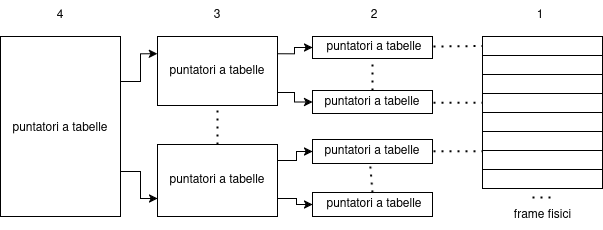
\includegraphics[scale=0.6]{../figures/mmu_trie.png}
\end{center}

Nei sistemi operativi moderni, quali Linux, ogni livello di accesso ha un nome specifico e quindi ogni segmento da 9 bit dei 36 bit di pagina rappresenta un informazione denominata diversamente, che riportiamo per completezza (dal più significativo):

\begin{table}[h!]
	\center \rowcolors{2}{white}{black!10}
	\begin{tabular} { c | c | p{7cm} }
		\bfseries Bit & \bfseries Nome & \bfseries Significato \\ 
		\hline
		9 bit & PML4I & \textit{Page Map Level 4 Index} \\
		9 bit & PDPTI & \textit{Page Directory Pointer Table Index} \\
		9 bit & PDI & \textit{Page Directory Index} \\
		9 bit & PTI & \textit{Page Table Index} \\
		12 bit & // & Offset di pagina 
	\end{tabular}
\end{table}

Resta comunque il fatto che quale nome decidiamo di assegnare alle tabelle di ogni livello di accesso non è importante, in quanto le strutture ad ogni livello sono sovrapposte (puntare a una tabella o a un frame è la stessa cosa).

Il procedimento che ci porta dai bit di pagina all'indirizzo del frame si chiama \textbf{table walk}, o \textit{cammino della tabella}.
Ogni entrata delle tabelle di trie sarà grande 8 byte (almeno 7 bit per i flag, più $\sim 48$ bit di indirizzo, ricordando che lo spazio indirizzabile nell'x86\_64 non corrisponde al massimo di 64 bit), per cui $2^9 \cdot 2^3 = 2^{12} = 4\text{ KiB}$ di memoria ciascuna.

\noindent
\begin{minipage}{\textwidth}
La memoria massima \textit{raggiunta ad} ogni livello e il numero di entrate \textit{raggiunta ad} ogni livello sono quindi:

\begin{table}[H]
	\center \rowcolors{2}{white}{black!10}
	\begin{tabular} { c | p{6cm} | p{6cm} }
		\bfseries Livello & \bfseries Memoria massima usata & \bfseries Numero di entrate \\ 
		\hline 
		4 & $2^9 \cdot 2^3 = 2^{12} = 4 \text{ KiB}$                       & $2^9 = 512$ \\
		3 & $2^9 \cdot 2^9 \cdot 2^3 = 2^{21} = 2 \text{ MiB}$             & $2^9 \cdot 2^9 = 2^{18} = 256 \text{ Ki}$ \\            
		2 & $2^9 \cdot 2^9 \cdot 2^9 \cdot 2^3 = 2^{30} = 1 \text{ GiB}$   & $2^9 \cdot 2^9 \cdot 2^9 = 2^{27} = 128 \text{ Mi}$ \\ 
		1 & $2^9 \cdot 2^9 \cdot 2^9 \cdot 2^9 \cdot 2^3 = 2^{39} = 512 \text{ GiB}$ & $2^9 \cdot 2^9 \cdot 2^9 \cdot 2^9 = 2^{36} = 64 \text{ Gi}$
	\end{tabular}
\end{table}
\end{minipage}
\par\bigskip

Per cottenere l'informazione inversa, cioè la memoria massima \textit{raggiungibile da} ogni livello e il numero di entrate \textit{raggiungibili da} ogni livelo basterà invertire l'ordine verticale delle ultime 2 colonne. 

Potremmo allora chiederci dov'è il guadagno di un sistema di questo tipo, in quanto a memoria l'ultimo livello di trie necessiterà degli stessi 512 GiB, più lo spazio necessario ai livelli precedenti.
Il vantaggio sarà però quello di poter tagliare arbitrariamente rami dall'albero che abbiamo formato, cioè non tenere conto di pagine di cui non abbiamo attualmente bisogno. 

\subsubsection{Descrittori nella T-MMU}
Vediamo come si evolvono i descrittori che avevamo messa corredo delle tabelle di corrispondenza, nella T-MMU.
Avremo che ci dovrà essere una distinzione fra i descrittori di primo e di secondo, terzo e quarto livello:
\begin{itemize}
	\item \textbf{Descrittori di primo livello:}
		qui vogliamo usare l'intero insieme di descrittori, che riportiamo:
\begin{center}
	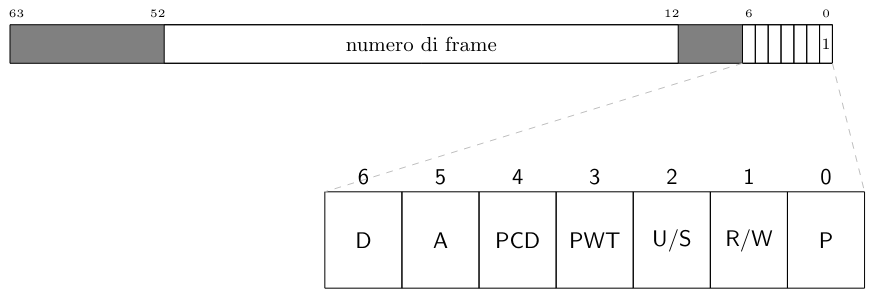
\includegraphics[scale=0.6]{../figures/mmu_level1.png}
\end{center}
\begin{itemize}
	\item \textbf{P:} un bit di presenza, che definisce l'esistenza o meno di una traduzione per quell'indirizzo: nel caso di accesso a pagine non traducibili si genera un ecceione, detta \textbf{page fault}, che comporta il caricamento della pagina richiesta o la terminazione forzata del programma per \textbf{segmentation fault}.

		Ad esempio, se scegliamo 0 come la codifica del null pointer, vogliamo che la prima pagina (o le prime pagine, se vogliamo essere più larghi con accessi a strutture puntate da null pointer, che potrebbero avere offset negli struct anche consideravoli) sia non presente, e quindi si traduca in eccezione prima di effettuare accessi chiaramente erronei;
	\item \textbf{S/U:} \textit{Sistema/Utente}, indica se una pagina è accessibile o meno ad un processo utente;  
	\item \textbf{R/W:} \textit{Read/Write}, indica se una pagina è accessibile solo in scrittura o solo in lettura per un certo processo. 
		Questa può essere utile ad esempio per la sezione \textit{text} del programma, che ricordiamo contiene il codice e non vogliamo venga modificata;
	\item \textbf{PCD} e \textbf{PWT}: indicano se ignorare completamente la cache (PCD) o se adottare una politica di scrittura \textit{write-through} (PWT).
		Questo può essere utile nel caso di dispositivi mappati in memoria (come l'APIC o l'adattatore video);
	\item \textbf{A} e \textbf{D}: due flag che danno indicazioni agli accessi che la MMU ha individuato sulla pagina.

		Vediamo solo adesso la loro utilità: la MMU setta questi bit per dare informazioni al kernel su cosa è successo alle pagine fino all'ultimo accesso.
		Il bit \textbf{A}, quindi, indica che una certa pagina è stata usata (\textit{attraversata}), mentre il bit \textbf{D} (\textit{Dirty}) indica che si è scritto su una certa pagina. 
		Abbiamo quindi una situazione dove è l'\textit{hardware} ad informare il \textit{software} del suo funzionamento, e non viceversa (come eravamo abituati). 
		L'informazione può quindi essere usata per gestire meglio il caricamento su e da memoria delle pagine, sopratutto in sistemi che supportano la \textit{memoria di swap}, cioè una certa porzione di memoria sul disco rigido che viene impiegata nella memorizzazione delle immagini dei processi in esecuzione (che è come, in origine, avevamo ipotizzato funzionasse il meccanismo della multiprogrammazione).
		In questo caso conoscere il flag D può evitare una scrittura su disco quando una pagina non è stata modificata, mentre conoscere il flag A può dare un euristica su quali pagine conviene spostare nello swap e quali mantenere nel caso di spostamento di pagine da e su disco.
		Per la precisione, in sistemi di questo tipo i pagefault sono normali, e vengono sfruttati per realizzare la \textit{paginazione su domanda}: può essere che la pagina richiesta da un processo non esista, quindi comporti un'eccezione, che viene gestita caricando la pagina corrispondente (e quindi verificando i flag A se altre pagine vanno rimosse per fare spazio).
\end{itemize}

	\item \textbf{Descrittori di secondo, terzo e quarto livello:} il descrittore ha questo aspetto:
\begin{center}
	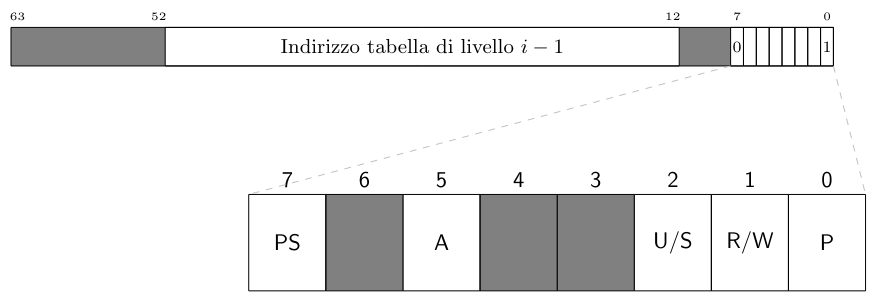
\includegraphics[scale=0.6]{../figures/mmu_level234.png}
\end{center}
		in questo caso non abbiamo bisogno di \textbf{PWT}, \textbf{PCT} e \textbf{D}, mentre introduciamo un nuovo bit, \textbf{PS}, \textit{Page Size}, che distingue due situazioni: se PS è basso, si procede come si è detto finora, altrimenti, quella entrata punta ad un unica pagina contigua di entrate (e non al livello successivo della trie).
		Il numero di entrate delle pagine contigue, dette \textbf{huge page}, cambia quindi in base al livello:
\begin{table}[H]
	\center \rowcolors{2}{white}{black!10}
	\begin{tabular} { c | p{6cm} }
		\bfseries Livello & \bfseries Memoria indirizzata in huge page\\ 
		\hline 
		4 & // \\ 
		3 & 1 GiB \\ 
		2 & 2 MiB \\ 
		1 & 4 Kib (default) \\
	\end{tabular}
\end{table}
in quanto, ad ogni livello, stiamo effettivamente "passando" 9 bit dall'indirizzo di pagina all'offset nella pagina, cioè stiamo adottando indirizzi e offset di dimensione:
\begin{table}[H]
	\center \rowcolors{2}{white}{black!10}
	\begin{tabular} { c | p{5cm} | p{5cm} }
		\bfseries Livello & \bfseries Dimensione indirizzo & \bfseries Dimensione offset \\ 
		\hline 
		4 & // & // \\ 
		3 & 18 bit & 30  bit \\
		2 & 27 bit & 21 bit \\ 
		1 & 36 bit & 12 bit \\
	\end{tabular}
\end{table}

Come si vede poi dalla tabella, il flag PS è effettivamente ignorato al livello 4 (avremmo pagine da 512 GB, che ad oggi non tornano particolarmente utili) e al livello 1 (è la dimensione di default delle pagine).
\end{itemize}

\subsubsection{T-MMU e memoria condivisa}
La struttura ad albero delle trie ci permette, ad esempio, di far puntare un entrata di un sottoalbero della trie associata ad un processo, ad un sottoalbero di una trie di un altro processo.
Questo ci permette effettivamente di realizzare pagine, o tabelle di pagine, condivise fra processi.
Potremo liberamente assegnare la stessa pagina in posizioni diverse dello spazio di memoria di ogni processo, in quanto l'unica cosa importante è il \textit{percorso} che ci porta alla tabella condivisa, che può variare di processo in processo (o meglio di trie di processo in trie di processo).

\end{document}


\documentclass[a4paper,11pt]{article}
\usepackage[a4paper, margin=8em]{geometry}

% usa i pacchetti per la scrittura in italiano
\usepackage[french,italian]{babel}
\usepackage[T1]{fontenc}
\usepackage[utf8]{inputenc}
\frenchspacing 

% usa i pacchetti per la formattazione matematica
\usepackage{amsmath, amssymb, amsthm, amsfonts}

% usa altri pacchetti
\usepackage{gensymb}
\usepackage{hyperref}
\usepackage{standalone}

\usepackage{colortbl}

\usepackage{xstring}
\usepackage{karnaugh-map}

% imposta il titolo
\title{Appunti Calcolatori Elettronici}
\author{Luca Seggiani}
\date{2025}

% imposta lo stile
% usa helvetica
\usepackage[scaled]{helvet}
% usa palatino
\usepackage{palatino}
% usa un font monospazio guardabile
\usepackage{lmodern}

\renewcommand{\rmdefault}{ppl}
\renewcommand{\sfdefault}{phv}
\renewcommand{\ttdefault}{lmtt}

% circuiti
\usepackage{circuitikz}
\usetikzlibrary{babel}

% testo cerchiato
\newcommand*\circled[1]{\tikz[baseline=(char.base)]{
            \node[shape=circle,draw,inner sep=2pt] (char) {#1};}}

% disponi il titolo
\makeatletter
\renewcommand{\maketitle} {
	\begin{center} 
		\begin{minipage}[t]{.8\textwidth}
			\textsf{\huge\bfseries \@title} 
		\end{minipage}%
		\begin{minipage}[t]{.2\textwidth}
			\raggedleft \vspace{-1.65em}
			\textsf{\small \@author} \vfill
			\textsf{\small \@date}
		\end{minipage}
		\par
	\end{center}

	\thispagestyle{empty}
	\pagestyle{fancy}
}
\makeatother

% disponi teoremi
\usepackage{tcolorbox}
\newtcolorbox[auto counter, number within=section]{theorem}[2][]{%
	colback=blue!10, 
	colframe=blue!40!black, 
	sharp corners=northwest,
	fonttitle=\sffamily\bfseries, 
	title=Teorema~\thetcbcounter: #2, 
	#1
}

% disponi definizioni
\newtcolorbox[auto counter, number within=section]{definition}[2][]{%
	colback=red!10,
	colframe=red!40!black,
	sharp corners=northwest,
	fonttitle=\sffamily\bfseries,
	title=Definizione~\thetcbcounter: #2,
	#1
}

% disponi codice
\usepackage{listings}
\usepackage[table]{xcolor}

\definecolor{codegreen}{rgb}{0,0.6,0}
\definecolor{codegray}{rgb}{0.5,0.5,0.5}
\definecolor{codepurple}{rgb}{0.58,0,0.82}
\definecolor{backcolour}{rgb}{0.95,0.95,0.92}

\lstdefinestyle{codestyle}{
		backgroundcolor=\color{black!5}, 
		commentstyle=\color{codegreen},
		keywordstyle=\bfseries\color{magenta},
		numberstyle=\sffamily\tiny\color{black!60},
		stringstyle=\color{green!50!black},
		basicstyle=\ttfamily\footnotesize,
		breakatwhitespace=false,         
		breaklines=true,                 
		captionpos=b,                    
		keepspaces=true,                 
		numbers=left,                    
		numbersep=5pt,                  
		showspaces=false,                
		showstringspaces=false,
		showtabs=false,                  
		tabsize=2
}

\lstdefinestyle{shellstyle}{
		backgroundcolor=\color{black!5}, 
		basicstyle=\ttfamily\footnotesize\color{black}, 
		commentstyle=\color{black}, 
		keywordstyle=\color{black},
		numberstyle=\color{black!5},
		stringstyle=\color{black}, 
		showspaces=false,
		showstringspaces=false, 
		showtabs=false, 
		tabsize=2, 
		numbers=none, 
		breaklines=true
}


\lstdefinelanguage{assembler}{ 
  keywords={AAA, AAD, AAM, AAS, ADC, ADCB, ADCW, ADCL, ADD, ADDB, ADDW, ADDL, AND, ANDB, ANDW, ANDL,
        ARPL, BOUND, BSF, BSFL, BSFW, BSR, BSRL, BSRW, BSWAP, BT, BTC, BTCB, BTCW, BTCL, BTR, 
        BTRB, BTRW, BTRL, BTS, BTSB, BTSW, BTSL, CALL, CBW, CDQ, CLC, CLD, CLI, CLTS, CMC, CMP,
        CMPB, CMPW, CMPL, CMPS, CMPSB, CMPSD, CMPSW, CMPXCHG, CMPXCHGB, CMPXCHGW, CMPXCHGL,
        CMPXCHG8B, CPUID, CWDE, DAA, DAS, DEC, DECB, DECW, DECL, DIV, DIVB, DIVW, DIVL, ENTER,
        HLT, IDIV, IDIVB, IDIVW, IDIVL, IMUL, IMULB, IMULW, IMULL, IN, INB, INW, INL, INC, INCB,
        INCW, INCL, INS, INSB, INSD, INSW, INT, INT3, INTO, INVD, INVLPG, IRET, IRETD, JA, JAE,
        JB, JBE, JC, JCXZ, JE, JECXZ, JG, JGE, JL, JLE, JMP, JNA, JNAE, JNB, JNBE, JNC, JNE, JNG,
        JNGE, JNL, JNLE, JNO, JNP, JNS, JNZ, JO, JP, JPE, JPO, JS, JZ, LAHF, LAR, LCALL, LDS,
        LEA, LEAVE, LES, LFS, LGDT, LGS, LIDT, LMSW, LOCK, LODSB, LODSD, LODSW, LOOP, LOOPE,
        LOOPNE, LSL, LSS, LTR, MOV, MOVB, MOVW, MOVL, MOVSB, MOVSD, MOVSW, MOVSX, MOVSXB,
        MOVSXW, MOVSXL, MOVZX, MOVZXB, MOVZXW, MOVZXL, MUL, MULB, MULW, MULL, NEG, NEGB, NEGW,
        NEGL, NOP, NOT, NOTB, NOTW, NOTL, OR, ORB, ORW, ORL, OUT, OUTB, OUTW, OUTL, OUTSB, OUTSD,
        OUTSW, POP, POPL, POPW, POPB, POPA, POPAD, POPF, POPFD, PUSH, PUSHL, PUSHW, PUSHB, PUSHA, 
				PUSHAD, PUSHF, PUSHFD, RCL, RCLB, RCLW, MOVSL, MOVSB, MOVSW, STOSL, STOSB, STOSW, LODSB, LODSW,
				LODSL, INSB, INSW, INSL, OUTSB, OUTSL, OUTSW
        RCLL, RCR, RCRB, RCRW, RCRL, RDMSR, RDPMC, RDTSC, REP, REPE, REPNE, RET, ROL, ROLB, ROLW,
        ROLL, ROR, RORB, RORW, RORL, SAHF, SAL, SALB, SALW, SALL, SAR, SARB, SARW, SARL, SBB,
        SBBB, SBBW, SBBL, SCASB, SCASD, SCASW, SETA, SETAE, SETB, SETBE, SETC, SETE, SETG, SETGE,
        SETL, SETLE, SETNA, SETNAE, SETNB, SETNBE, SETNC, SETNE, SETNG, SETNGE, SETNL, SETNLE,
        SETNO, SETNP, SETNS, SETNZ, SETO, SETP, SETPE, SETPO, SETS, SETZ, SGDT, SHL, SHLB, SHLW,
        SHLL, SHLD, SHR, SHRB, SHRW, SHRL, SHRD, SIDT, SLDT, SMSW, STC, STD, STI, STOSB, STOSD,
        STOSW, STR, SUB, SUBB, SUBW, SUBL, TEST, TESTB, TESTW, TESTL, VERR, VERW, WAIT, WBINVD,
        XADD, XADDB, XADDW, XADDL, XCHG, XCHGB, XCHGW, XCHGL, XLAT, XLATB, XOR, XORB, XORW, XORL},
  keywordstyle=\color{blue}\bfseries,
  ndkeywordstyle=\color{darkgray}\bfseries,
  identifierstyle=\color{black},
  sensitive=false,
  comment=[l]{\#},
  morecomment=[s]{/*}{*/},
  commentstyle=\color{purple}\ttfamily,
  stringstyle=\color{red}\ttfamily,
  morestring=[b]',
  morestring=[b]"
}

\lstset{language=assembler, style=codestyle}

% disponi sezioni
\usepackage{titlesec}

\titleformat{\section}
	{\sffamily\Large\bfseries} 
	{\thesection}{1em}{} 
\titleformat{\subsection}
	{\sffamily\large\bfseries}   
	{\thesubsection}{1em}{} 
\titleformat{\subsubsection}
	{\sffamily\normalsize\bfseries} 
	{\thesubsubsection}{1em}{}

% tikz
\usepackage{tikz}

% float
\usepackage{float}

% grafici
\usepackage{pgfplots}
\pgfplotsset{width=10cm,compat=1.9}

% disponi alberi
\usepackage{forest}

\forestset{
	rectstyle/.style={
		for tree={rectangle,draw,font=\large\sffamily}
	},
	roundstyle/.style={
		for tree={circle,draw,font=\large}
	}
}

% disponi algoritmi
\usepackage{algorithm}
\usepackage{algorithmic}
\makeatletter
\renewcommand{\ALG@name}{Algoritmo}
\makeatother

% disponi numeri di pagina
\usepackage{fancyhdr}
\fancyhf{} 
\fancyfoot[L]{\sffamily{\thepage}}

\makeatletter
\fancyhead[L]{\raisebox{1ex}[0pt][0pt]{\sffamily{\@title \ \@date}}} 
\fancyhead[R]{\raisebox{1ex}[0pt][0pt]{\sffamily{\@author}}}
\makeatother

\begin{document}
% sezione (data)
\section{Lezione del 01-04-25}

% stili pagina
\thispagestyle{empty}
\pagestyle{fancy}

% testo


\end{document}

\documentclass[a4paper,11pt]{article}
\usepackage[a4paper, margin=8em]{geometry}

% usa i pacchetti per la scrittura in italiano
\usepackage[french,italian]{babel}
\usepackage[T1]{fontenc}
\usepackage[utf8]{inputenc}
\frenchspacing 

% usa i pacchetti per la formattazione matematica
\usepackage{amsmath, amssymb, amsthm, amsfonts}

% usa altri pacchetti
\usepackage{gensymb}
\usepackage{hyperref}
\usepackage{standalone}

\usepackage{colortbl}

\usepackage{xstring}
\usepackage{karnaugh-map}

% imposta il titolo
\title{Appunti Calcolatori Elettronici}
\author{Luca Seggiani}
\date{2025}

% imposta lo stile
% usa helvetica
\usepackage[scaled]{helvet}
% usa palatino
\usepackage{palatino}
% usa un font monospazio guardabile
\usepackage{lmodern}

\renewcommand{\rmdefault}{ppl}
\renewcommand{\sfdefault}{phv}
\renewcommand{\ttdefault}{lmtt}

% circuiti
\usepackage{circuitikz}
\usetikzlibrary{babel}

% testo cerchiato
\newcommand*\circled[1]{\tikz[baseline=(char.base)]{
            \node[shape=circle,draw,inner sep=2pt] (char) {#1};}}

% disponi il titolo
\makeatletter
\renewcommand{\maketitle} {
	\begin{center} 
		\begin{minipage}[t]{.8\textwidth}
			\textsf{\huge\bfseries \@title} 
		\end{minipage}%
		\begin{minipage}[t]{.2\textwidth}
			\raggedleft \vspace{-1.65em}
			\textsf{\small \@author} \vfill
			\textsf{\small \@date}
		\end{minipage}
		\par
	\end{center}

	\thispagestyle{empty}
	\pagestyle{fancy}
}
\makeatother

% disponi teoremi
\usepackage{tcolorbox}
\newtcolorbox[auto counter, number within=section]{theorem}[2][]{%
	colback=blue!10, 
	colframe=blue!40!black, 
	sharp corners=northwest,
	fonttitle=\sffamily\bfseries, 
	title=Teorema~\thetcbcounter: #2, 
	#1
}

% disponi definizioni
\newtcolorbox[auto counter, number within=section]{definition}[2][]{%
	colback=red!10,
	colframe=red!40!black,
	sharp corners=northwest,
	fonttitle=\sffamily\bfseries,
	title=Definizione~\thetcbcounter: #2,
	#1
}

% disponi codice
\usepackage{listings}
\usepackage[table]{xcolor}

\definecolor{codegreen}{rgb}{0,0.6,0}
\definecolor{codegray}{rgb}{0.5,0.5,0.5}
\definecolor{codepurple}{rgb}{0.58,0,0.82}
\definecolor{backcolour}{rgb}{0.95,0.95,0.92}

\lstdefinestyle{codestyle}{
		backgroundcolor=\color{black!5}, 
		commentstyle=\color{codegreen},
		keywordstyle=\bfseries\color{magenta},
		numberstyle=\sffamily\tiny\color{black!60},
		stringstyle=\color{green!50!black},
		basicstyle=\ttfamily\footnotesize,
		breakatwhitespace=false,         
		breaklines=true,                 
		captionpos=b,                    
		keepspaces=true,                 
		numbers=left,                    
		numbersep=5pt,                  
		showspaces=false,                
		showstringspaces=false,
		showtabs=false,                  
		tabsize=2
}

\lstdefinestyle{shellstyle}{
		backgroundcolor=\color{black!5}, 
		basicstyle=\ttfamily\footnotesize\color{black}, 
		commentstyle=\color{black}, 
		keywordstyle=\color{black},
		numberstyle=\color{black!5},
		stringstyle=\color{black}, 
		showspaces=false,
		showstringspaces=false, 
		showtabs=false, 
		tabsize=2, 
		numbers=none, 
		breaklines=true
}


\lstdefinelanguage{assembler}{ 
  keywords={AAA, AAD, AAM, AAS, ADC, ADCB, ADCW, ADCL, ADD, ADDB, ADDW, ADDL, AND, ANDB, ANDW, ANDL,
        ARPL, BOUND, BSF, BSFL, BSFW, BSR, BSRL, BSRW, BSWAP, BT, BTC, BTCB, BTCW, BTCL, BTR, 
        BTRB, BTRW, BTRL, BTS, BTSB, BTSW, BTSL, CALL, CBW, CDQ, CLC, CLD, CLI, CLTS, CMC, CMP,
        CMPB, CMPW, CMPL, CMPS, CMPSB, CMPSD, CMPSW, CMPXCHG, CMPXCHGB, CMPXCHGW, CMPXCHGL,
        CMPXCHG8B, CPUID, CWDE, DAA, DAS, DEC, DECB, DECW, DECL, DIV, DIVB, DIVW, DIVL, ENTER,
        HLT, IDIV, IDIVB, IDIVW, IDIVL, IMUL, IMULB, IMULW, IMULL, IN, INB, INW, INL, INC, INCB,
        INCW, INCL, INS, INSB, INSD, INSW, INT, INT3, INTO, INVD, INVLPG, IRET, IRETD, JA, JAE,
        JB, JBE, JC, JCXZ, JE, JECXZ, JG, JGE, JL, JLE, JMP, JNA, JNAE, JNB, JNBE, JNC, JNE, JNG,
        JNGE, JNL, JNLE, JNO, JNP, JNS, JNZ, JO, JP, JPE, JPO, JS, JZ, LAHF, LAR, LCALL, LDS,
        LEA, LEAVE, LES, LFS, LGDT, LGS, LIDT, LMSW, LOCK, LODSB, LODSD, LODSW, LOOP, LOOPE,
        LOOPNE, LSL, LSS, LTR, MOV, MOVB, MOVW, MOVL, MOVSB, MOVSD, MOVSW, MOVSX, MOVSXB,
        MOVSXW, MOVSXL, MOVZX, MOVZXB, MOVZXW, MOVZXL, MUL, MULB, MULW, MULL, NEG, NEGB, NEGW,
        NEGL, NOP, NOT, NOTB, NOTW, NOTL, OR, ORB, ORW, ORL, OUT, OUTB, OUTW, OUTL, OUTSB, OUTSD,
        OUTSW, POP, POPL, POPW, POPB, POPA, POPAD, POPF, POPFD, PUSH, PUSHL, PUSHW, PUSHB, PUSHA, 
				PUSHAD, PUSHF, PUSHFD, RCL, RCLB, RCLW, MOVSL, MOVSB, MOVSW, STOSL, STOSB, STOSW, LODSB, LODSW,
				LODSL, INSB, INSW, INSL, OUTSB, OUTSL, OUTSW
        RCLL, RCR, RCRB, RCRW, RCRL, RDMSR, RDPMC, RDTSC, REP, REPE, REPNE, RET, ROL, ROLB, ROLW,
        ROLL, ROR, RORB, RORW, RORL, SAHF, SAL, SALB, SALW, SALL, SAR, SARB, SARW, SARL, SBB,
        SBBB, SBBW, SBBL, SCASB, SCASD, SCASW, SETA, SETAE, SETB, SETBE, SETC, SETE, SETG, SETGE,
        SETL, SETLE, SETNA, SETNAE, SETNB, SETNBE, SETNC, SETNE, SETNG, SETNGE, SETNL, SETNLE,
        SETNO, SETNP, SETNS, SETNZ, SETO, SETP, SETPE, SETPO, SETS, SETZ, SGDT, SHL, SHLB, SHLW,
        SHLL, SHLD, SHR, SHRB, SHRW, SHRL, SHRD, SIDT, SLDT, SMSW, STC, STD, STI, STOSB, STOSD,
        STOSW, STR, SUB, SUBB, SUBW, SUBL, TEST, TESTB, TESTW, TESTL, VERR, VERW, WAIT, WBINVD,
        XADD, XADDB, XADDW, XADDL, XCHG, XCHGB, XCHGW, XCHGL, XLAT, XLATB, XOR, XORB, XORW, XORL},
  keywordstyle=\color{blue}\bfseries,
  ndkeywordstyle=\color{darkgray}\bfseries,
  identifierstyle=\color{black},
  sensitive=false,
  comment=[l]{\#},
  morecomment=[s]{/*}{*/},
  commentstyle=\color{purple}\ttfamily,
  stringstyle=\color{red}\ttfamily,
  morestring=[b]',
  morestring=[b]"
}

\lstset{language=assembler, style=codestyle}

% disponi sezioni
\usepackage{titlesec}

\titleformat{\section}
	{\sffamily\Large\bfseries} 
	{\thesection}{1em}{} 
\titleformat{\subsection}
	{\sffamily\large\bfseries}   
	{\thesubsection}{1em}{} 
\titleformat{\subsubsection}
	{\sffamily\normalsize\bfseries} 
	{\thesubsubsection}{1em}{}

% tikz
\usepackage{tikz}

% float
\usepackage{float}

% grafici
\usepackage{pgfplots}
\pgfplotsset{width=10cm,compat=1.9}

% disponi alberi
\usepackage{forest}

\forestset{
	rectstyle/.style={
		for tree={rectangle,draw,font=\large\sffamily}
	},
	roundstyle/.style={
		for tree={circle,draw,font=\large}
	}
}

% disponi algoritmi
\usepackage{algorithm}
\usepackage{algorithmic}
\makeatletter
\renewcommand{\ALG@name}{Algoritmo}
\makeatother

% disponi numeri di pagina
\usepackage{fancyhdr}
\fancyhf{} 
\fancyfoot[L]{\sffamily{\thepage}}

\makeatletter
\fancyhead[L]{\raisebox{1ex}[0pt][0pt]{\sffamily{\@title \ \@date}}} 
\fancyhead[R]{\raisebox{1ex}[0pt][0pt]{\sffamily{\@author}}}
\makeatother

\begin{document}
% sezione (data)
\section{Lezione del 04-04-25}

% stili pagina
\thispagestyle{empty}
\pagestyle{fancy}

% testo
\subsection{Funzioni di supporto alla paginazione}
Riprendiamo la trattazione della memoria virtuale paginata, discutendo quali funzioni il kernel studiato mette a supporto della sua operazione.

\subsubsection{Funzioni sugli indirizzi}
Nell'architettura x86\_64 un indirizzo, virtuale o fisico, sta su 64 bit, e quindi definiamo i tipi \lstinline|vaddr| e \lstinline|paddr|:
\begin{lstlisting}[language=C++, style=codestyle]	
typedef natq /* (uint64_t) */ vaddr; // indirizzo virtuale
typedef natq /*    idem    */ paddr; // indirizzo fisico 
\end{lstlisting}

Dotiamoci quindi di alcune funzioni per la gestione di questi indirizzi.
Di base, vorremmo un modo per verificare la normalizzazione di un indirizzo (quindi il fatto che i bit dal 48 al 63 siano uguali al bit 47, che possiamo fare con la \lstinline|norm(vaddr)|):
\begin{lstlisting}[language=C++, style=codestyle]	
if(norm(v) != v) {
	// errore: indirizzo non normalizzato
}
\end{lstlisting}

Definiamo poi due funzioni per trovare l'indirizzo della prima pagina contenuta e della prima pagina immediatamente dopo una regione di memoria $[x, y]$.
Avevamo trattato questo problema nella sezione 2.1.3, e usando quanto avevamo detto possiamo definire le funzioni \lstinline|base(vaddr)| e \lstinline|limit(vaddr)|.
\begin{lstlisting}[language=C++, style=codestyle]	
vaddr base(vaddr v, int liv)
{
	natq mask = dim_region(liv) - 1;
	return v & ~mask;
}

vaddr limit(vaddr v, int liv)
{
	natq dr = dim_region(liv);
	natq mask = dr - 1;
	return (v + dr - 1) & ~mask;
}
\end{lstlisting}
dove notiamo che l'indice di pagina resta comunque nei 36 (o meno nel caso di huge page) bit dedicati al numero di pagina (nel caso più semplice, azzeriamo i 12 bit di offset di pagina). 

La funzione helper \lstinline|dim_region(int)| calcola la dimensione di una pagina ad un certo livello di paginazione (sui i livelli $4, 3, 2, 1$, indicati come $3, 2, 1, 0$), ed è definita come:
\begin{lstlisting}[language=C++, style=codestyle]	
natq dim_region(int liv)
{
	natq v = 1ULL << (liv * 9 + 12);
	return v;
}
\end{lstlisting}

\subsubsection{Funzioni sulle tabelle}
Un singolo descrittore di tabella viene rappresentato dal tipo \lstinline|tab_entry|, che entra (come abbiamo visto nella sezione 14.0.3) in 64 bit, per cui possiamo dire:
\begin{lstlisting}[language=C++, style=codestyle]	
typedef natq /* (uint64_t) */ tab_entry;
\end{lstlisting}

L'interazione vera e propria con il descrittore avverrà attraverso maschere e funzioni che applicano maschere.
Ad esempio, se per modificare il bit di presenza di una pagina si può dire:
\begin{lstlisting}[language=C++, style=codestyle]	
// e e' un riferimento ad una tabella
e |= BIT_P; // BIT_P maschera il bit di presenza
\end{lstlisting}
mentre se si vuole estrarre o modificare l'indirizzo fisico si possono sfruttare rispettivamente le funzioni \lstinline|extr_IND_FISICO(tab_entry)| e \lstinline|set_IND_FISICO(tab_entry)|:
\begin{lstlisting}[language=C++, style=codestyle]	
// e e' un riferimento ad una tabella
paddr p;

// prendi l'indirizzo fisico di e
p = extr_IND_FISICO(e);

// per esempio, rimetticelo
set_IND_FISICO(e, p);
\end{lstlisting}

Esiste poi le funzione \lstinline|i_tab(vaddr v, int liv)| per l'accesso alla regione da 9 bit che indirizza le tabelle di livello \lstinline|liv| di un indirizzo \lstinline|v|.
Questa potrà essere usata con le funzioni \lstinline|get_entry(paddr, int)| e \lstinline|set_entry(paddr, int, tab_entry)|, che si occupano rispettivamente di ottenere un entrata di una tabella e modificarne una, sostituendo l'intero descrittore.

Ad esempio, potremo dire:
\begin{lstlisting}[language=C++, style=codestyle]	
// questo e' un indirizzo, diciamo che la tabella tab e' di livello 2
vaddr v;

// e e' un descrittore di tabella di livello 1 
tab_entry& e = get_entry(tab, i_tab(v, 2));

// creiamo un descrittore per sostituire e
tab_entry se;
// ... imposta se

// modifica la stessa entrata
set_entry(tab, i_tab(v, 2), se);
\end{lstlisting}

Copie o sovrascritture in massa si possono fare poi con le funzioni \lstinline|copy_des()| e \lstinline|set_des()|, che per adesso non vediamo nel dettaglio.

\subsubsection{Funzioni sulla MMU}
Notiamo l'esistenza della \lstinline|loadCR3()| per l'attivazione di un nuovo albero di traduzione, che carica un indirizzo fisico nel registro \lstinline|CR3|, e \lstinline|readCR3()|, che permette successivamente di rileggerlo.

Esiste anche la \lstinline|readCR2()|, che permette la lettura di \lstinline|CR2|, dove si trova l'ultimo indirizzo la cui traduzione ha causato un pagefault.

Esistono poi le funzioni di interazione con il TLB: \lstinline|invalida_entrata_TLB(vaddr v)| permette di invalidare l'indirizzo virtuale \lstinline|v| sfruttando l'istruzione assembler \lstinline|INVLPG|, mentre \lstinline|invalida_TLB()| invalida l'intero albero di traduzione (cosa che ricordiamo faceva già la \lstinline|loadCR3()|).

\subsubsection{Iteratori di tabella}
La gestione ad alto livello dei trie (\textit{alberi di traduzione}) viene effettuata sfruttando l'iteratore \lstinline|tab_iter|.

Questo serve per effettuare visite in diversi ordini (che vederemo fra poco), a livello di \textit{pagina}: l'offset di pagina andrà comunque conservato a parte, in quanto l'iteratore ci porterà, al massimo, solo fino all'indirizzo fisico della pagina giusta.
Sui \lstinline|tab_iter| sono definite alcune funzioni membro: le \lstinline|get_e()|, \lstinline|get_tab()| e \lstinline|get_l()| permettono di ottenere, rispettivamente, un riferimento all’entrata su cui si trova l’iteratore, l’indirizzo fisico della tabella che contiene questa entrata e il livello (4, 3, 2 o 1) di questa tabella. 
La funzione \lstinline|get_v()|, invece, restituisce il più piccolo indirizzo virtuale la cui traduzione passa da questa entrata.

Il \lstinline|tab_iter| viene inizializzato attraverso un indirizzo virtuale, o una coppia di questi in modo da esplorare un intera regione di indirizzi virtuali.
Una volta definito un'oggetto \lstinline|tab_iter|, si possono sfruttare le funzioni \lstinline|up|, \lstinline|down| e \lstinline|right| per spostarsi rispettivamente nella tabella di livello superiore, inferiore, e a destra fra le tabelle di livello corrente.
La funzione \lstinline|done()|, che si ottiene anche dall'operatore di conversione a \lstinline|bool|, restituisce falso quando la visita è terminata (siamo arrivati alla pagina o non possiamo proseguire).

Attraverso queste funzioni, e alle \lstinline|next()| (che avanza l'iteratore in avanti in visita anticipata, cercando di raggiungere il prossimo indirizzo) e \lstinline|next_post()| (che avanza l'iteratore in avanti in visita posticipata) si possono realizzare quindi diversi tipi di visita ad un trie, fra cui:
\begin{itemize}
	\item \textbf{Visita anticipata di un singolo indirizzo:} si percorre l'intero percorso di traduzione di un indirizzo \lstinline|v| come segue:
\begin{lstlisting}[language=C++, style=codestyle]	
for(tab_iter it(tab, v); it; it.next()) {
	// it e' l'elemento corrente
}
\end{lstlisting}

Una soluzione alternativa si ha sfruttando direttamente \lstinline|down()|:
\begin{lstlisting}[language=C++, style=codestyle]	
tab_iter it(tab, v);
while (it.down()) {
	// it e' l'elemento corrente
}
\end{lstlisting}

	\item \textbf{Visita anticipata di una regione di indirizzi:} analoga a sopra, ma si forniscono entrambi gli indirizzi al costruttore del \lstinline|tab_iter|: 
\begin{lstlisting}[language=C++, style=codestyle]	
for(tab_iter it(tab, v_lo, v_hi); it; it.next()) {
	// it e' l'elemento corrente
}
\end{lstlisting}
	
	\item \textbf{Visita posticipata di una regione di indirizzi:} ancora analoga a sopra, ma si scende del tutto sfruttando la \lstinline|post()|, e poi si prosegue con la \lstinline|next_post()|: 
\begin{lstlisting}[language=C++, style=codestyle]	
tab_iter it(tab, v);
for (it.post(); it; it.next_post()} {
	// it e' l'elemento corrente
}
\end{lstlisting}

Notiamo che la \lstinline|post()| non implementa altro che la visita anticipata che abbiamo visto prima:
\begin{lstlisting}[language=C++, style=codestyle]	
void tab_iter::post()
{
	// controlli di validita'
	if (done())
		return;

	while (down())
		;
}
\end{lstlisting}

\end{itemize}

\subsubsection{Trasformazione}
Possiamo quindi definire la funzione \lstinline|trasforma(paddr, vaddr)| che usa l'albero di traduzione puntato dall'indirizzo fisico al primo argomento per tradurre, in un altro indirizzo fisico, l'indirizzo virtuale al secondo argomento.
Solitamente l'albero di traduzione che ci interesserà sara quello attualmente caricato in \lstinline|readCR3()|, cioè:
\begin{lstlisting}[language=C++, style=codestyle]	
// v e' un indirizzo virtuale
paddr p = trasforma(readCR3(), v);
\end{lstlisting}

L'implementazione della \lstinline|trasforma()| si riduce effettivamente a:
\begin{enumerate}
	\item Esegui una visita in ordine anticipato fino alla pagina corretta;
	\item Verifica se la pagina è stata effettivamente ottenuta (altrimenti restituisci l'indirizzo 0);
	\item Combina l'indirizzo fisico di pagina con l'offset di pagina. 
\end{enumerate}
cioè in codice:
\begin{lstlisting}[language=C++, style=codestyle]	
paddr trasforma(paddr root_tab, vaddr v)
{
	// punto 1
	tab_iter it(root_tab, v);
	while (it.down())
		;

	// punto 2
	tab_entry e = it.get_e();
	if (!(e & BIT_P))
		return 0;

	// punto 3 (con un dettaglio riguardante le huge page: si prende come offset la maschera ottenuta da dim_region())
	int l = it.get_l();
	natq mask = dim_region(l - 1) - 1;
	return (e & ~mask) | (v & mask);
}
\end{lstlisting}

\subsubsection{map() e unmap()}
Vediamo infine due funzioni che permettono di mappare e liberare regioni di memoria contigue nello spazio virtuale, ottenendo attraverso un qualche helper \lstinline|alloca_tab()| nuovi frame fisici (anche non contigui) e rilasciandoli con \lstinline|rilascia_tab()|.
Queste sono la \lstinline|map()| e la \lstinline|unmap()|.

La chiamata della \lstinline|map()| è:
\begin{lstlisting}[language=C++, style=codestyle]	
vaddr map(paddr tab, vaddr begin, vaddr end, natl flags, T& getpaddr, int ps_lvl = 1)
\end{lstlisting}
cioè dobbiamo specificare la tabella madre, gli indirizzi virtuali di confine della regione, una double word contenente eventuali flag R/W o U/S, e una funzione per l'ottenimento sequenziale di indirizzi fisici, che viene passata come \textit{funtore} o come \textit{lambda} (non si entra nei dettagli dello standard C++, va bene una funzione come una classe che ridefinisce l'operatore di chiamata).

La chiamata della \lstinline|unmap()| è invece:
\begin{lstlisting}[language=C++, style=codestyle]	
void unmap(paddr tab, vaddr begin, vaddr end, T& putpaddr)
\end{lstlisting}
dove vediamo servono principalmente gli stessi parametri, più la funzione \lstinline|putpaddr()|, che può essere usata per fare pulizia degli indirizzi fisici non più usati.

Ad esempio, se questi vengono posti in memoria dinamica attraverso l'helper passato a \lstinline|getpaddr| della \lstinline|map()|, e si sfrutta qualche struttura dati che tiene conto di quali regioni di memoria fisica sono effettivamente in utilizzo, il parametro \lstinline|putpaddr()| ci permette di definire una funzione che ripulisca i frame utilizzati una volta che questi vengono liberati, liberando le pagine di memoria corrispondente.

Un'ultima precisazione va fatta riguardo alle funzioni usate da \lstinline|map()| e \lstinline|unmap()|: queste saranno la \lstinline|copy_des()| e la \lstinline|set_des()| che avevamo visto in 16.1.2, più ottimizzate per la modifica in massa.

\end{document}


\documentclass[a4paper,11pt]{article}
\usepackage[a4paper, margin=8em]{geometry}

% usa i pacchetti per la scrittura in italiano
\usepackage[french,italian]{babel}
\usepackage[T1]{fontenc}
\usepackage[utf8]{inputenc}
\frenchspacing 

% usa i pacchetti per la formattazione matematica
\usepackage{amsmath, amssymb, amsthm, amsfonts}

% usa altri pacchetti
\usepackage{gensymb}
\usepackage{hyperref}
\usepackage{standalone}

\usepackage{colortbl}

\usepackage{xstring}
\usepackage{karnaugh-map}

% imposta il titolo
\title{Appunti Calcolatori Elettronici}
\author{Luca Seggiani}
\date{2025}

% imposta lo stile
% usa helvetica
\usepackage[scaled]{helvet}
% usa palatino
\usepackage{palatino}
% usa un font monospazio guardabile
\usepackage{lmodern}

\renewcommand{\rmdefault}{ppl}
\renewcommand{\sfdefault}{phv}
\renewcommand{\ttdefault}{lmtt}

% circuiti
\usepackage{circuitikz}
\usetikzlibrary{babel}

% testo cerchiato
\newcommand*\circled[1]{\tikz[baseline=(char.base)]{
            \node[shape=circle,draw,inner sep=2pt] (char) {#1};}}

% disponi il titolo
\makeatletter
\renewcommand{\maketitle} {
	\begin{center} 
		\begin{minipage}[t]{.8\textwidth}
			\textsf{\huge\bfseries \@title} 
		\end{minipage}%
		\begin{minipage}[t]{.2\textwidth}
			\raggedleft \vspace{-1.65em}
			\textsf{\small \@author} \vfill
			\textsf{\small \@date}
		\end{minipage}
		\par
	\end{center}

	\thispagestyle{empty}
	\pagestyle{fancy}
}
\makeatother

% disponi teoremi
\usepackage{tcolorbox}
\newtcolorbox[auto counter, number within=section]{theorem}[2][]{%
	colback=blue!10, 
	colframe=blue!40!black, 
	sharp corners=northwest,
	fonttitle=\sffamily\bfseries, 
	title=Teorema~\thetcbcounter: #2, 
	#1
}

% disponi definizioni
\newtcolorbox[auto counter, number within=section]{definition}[2][]{%
	colback=red!10,
	colframe=red!40!black,
	sharp corners=northwest,
	fonttitle=\sffamily\bfseries,
	title=Definizione~\thetcbcounter: #2,
	#1
}

% disponi codice
\usepackage{listings}
\usepackage[table]{xcolor}

\definecolor{codegreen}{rgb}{0,0.6,0}
\definecolor{codegray}{rgb}{0.5,0.5,0.5}
\definecolor{codepurple}{rgb}{0.58,0,0.82}
\definecolor{backcolour}{rgb}{0.95,0.95,0.92}

\lstdefinestyle{codestyle}{
		backgroundcolor=\color{black!5}, 
		commentstyle=\color{codegreen},
		keywordstyle=\bfseries\color{magenta},
		numberstyle=\sffamily\tiny\color{black!60},
		stringstyle=\color{green!50!black},
		basicstyle=\ttfamily\footnotesize,
		breakatwhitespace=false,         
		breaklines=true,                 
		captionpos=b,                    
		keepspaces=true,                 
		numbers=left,                    
		numbersep=5pt,                  
		showspaces=false,                
		showstringspaces=false,
		showtabs=false,                  
		tabsize=2
}

\lstdefinestyle{shellstyle}{
		backgroundcolor=\color{black!5}, 
		basicstyle=\ttfamily\footnotesize\color{black}, 
		commentstyle=\color{black}, 
		keywordstyle=\color{black},
		numberstyle=\color{black!5},
		stringstyle=\color{black}, 
		showspaces=false,
		showstringspaces=false, 
		showtabs=false, 
		tabsize=2, 
		numbers=none, 
		breaklines=true
}


\lstdefinelanguage{assembler}{ 
  keywords={AAA, AAD, AAM, AAS, ADC, ADCB, ADCW, ADCL, ADD, ADDB, ADDW, ADDL, AND, ANDB, ANDW, ANDL,
        ARPL, BOUND, BSF, BSFL, BSFW, BSR, BSRL, BSRW, BSWAP, BT, BTC, BTCB, BTCW, BTCL, BTR, 
        BTRB, BTRW, BTRL, BTS, BTSB, BTSW, BTSL, CALL, CBW, CDQ, CLC, CLD, CLI, CLTS, CMC, CMP,
        CMPB, CMPW, CMPL, CMPS, CMPSB, CMPSD, CMPSW, CMPXCHG, CMPXCHGB, CMPXCHGW, CMPXCHGL,
        CMPXCHG8B, CPUID, CWDE, DAA, DAS, DEC, DECB, DECW, DECL, DIV, DIVB, DIVW, DIVL, ENTER,
        HLT, IDIV, IDIVB, IDIVW, IDIVL, IMUL, IMULB, IMULW, IMULL, IN, INB, INW, INL, INC, INCB,
        INCW, INCL, INS, INSB, INSD, INSW, INT, INT3, INTO, INVD, INVLPG, IRET, IRETD, JA, JAE,
        JB, JBE, JC, JCXZ, JE, JECXZ, JG, JGE, JL, JLE, JMP, JNA, JNAE, JNB, JNBE, JNC, JNE, JNG,
        JNGE, JNL, JNLE, JNO, JNP, JNS, JNZ, JO, JP, JPE, JPO, JS, JZ, LAHF, LAR, LCALL, LDS,
        LEA, LEAVE, LES, LFS, LGDT, LGS, LIDT, LMSW, LOCK, LODSB, LODSD, LODSW, LOOP, LOOPE,
        LOOPNE, LSL, LSS, LTR, MOV, MOVB, MOVW, MOVL, MOVSB, MOVSD, MOVSW, MOVSX, MOVSXB,
        MOVSXW, MOVSXL, MOVZX, MOVZXB, MOVZXW, MOVZXL, MUL, MULB, MULW, MULL, NEG, NEGB, NEGW,
        NEGL, NOP, NOT, NOTB, NOTW, NOTL, OR, ORB, ORW, ORL, OUT, OUTB, OUTW, OUTL, OUTSB, OUTSD,
        OUTSW, POP, POPL, POPW, POPB, POPA, POPAD, POPF, POPFD, PUSH, PUSHL, PUSHW, PUSHB, PUSHA, 
				PUSHAD, PUSHF, PUSHFD, RCL, RCLB, RCLW, MOVSL, MOVSB, MOVSW, STOSL, STOSB, STOSW, LODSB, LODSW,
				LODSL, INSB, INSW, INSL, OUTSB, OUTSL, OUTSW
        RCLL, RCR, RCRB, RCRW, RCRL, RDMSR, RDPMC, RDTSC, REP, REPE, REPNE, RET, ROL, ROLB, ROLW,
        ROLL, ROR, RORB, RORW, RORL, SAHF, SAL, SALB, SALW, SALL, SAR, SARB, SARW, SARL, SBB,
        SBBB, SBBW, SBBL, SCASB, SCASD, SCASW, SETA, SETAE, SETB, SETBE, SETC, SETE, SETG, SETGE,
        SETL, SETLE, SETNA, SETNAE, SETNB, SETNBE, SETNC, SETNE, SETNG, SETNGE, SETNL, SETNLE,
        SETNO, SETNP, SETNS, SETNZ, SETO, SETP, SETPE, SETPO, SETS, SETZ, SGDT, SHL, SHLB, SHLW,
        SHLL, SHLD, SHR, SHRB, SHRW, SHRL, SHRD, SIDT, SLDT, SMSW, STC, STD, STI, STOSB, STOSD,
        STOSW, STR, SUB, SUBB, SUBW, SUBL, TEST, TESTB, TESTW, TESTL, VERR, VERW, WAIT, WBINVD,
        XADD, XADDB, XADDW, XADDL, XCHG, XCHGB, XCHGW, XCHGL, XLAT, XLATB, XOR, XORB, XORW, XORL},
  keywordstyle=\color{blue}\bfseries,
  ndkeywordstyle=\color{darkgray}\bfseries,
  identifierstyle=\color{black},
  sensitive=false,
  comment=[l]{\#},
  morecomment=[s]{/*}{*/},
  commentstyle=\color{purple}\ttfamily,
  stringstyle=\color{red}\ttfamily,
  morestring=[b]',
  morestring=[b]"
}

\lstset{language=assembler, style=codestyle}

% disponi sezioni
\usepackage{titlesec}

\titleformat{\section}
	{\sffamily\Large\bfseries} 
	{\thesection}{1em}{} 
\titleformat{\subsection}
	{\sffamily\large\bfseries}   
	{\thesubsection}{1em}{} 
\titleformat{\subsubsection}
	{\sffamily\normalsize\bfseries} 
	{\thesubsubsection}{1em}{}

% tikz
\usepackage{tikz}

% float
\usepackage{float}

% grafici
\usepackage{pgfplots}
\pgfplotsset{width=10cm,compat=1.9}

% disponi alberi
\usepackage{forest}

\forestset{
	rectstyle/.style={
		for tree={rectangle,draw,font=\large\sffamily}
	},
	roundstyle/.style={
		for tree={circle,draw,font=\large}
	}
}

% disponi algoritmi
\usepackage{algorithm}
\usepackage{algorithmic}
\makeatletter
\renewcommand{\ALG@name}{Algoritmo}
\makeatother

% disponi numeri di pagina
\usepackage{fancyhdr}
\fancyhf{} 
\fancyfoot[L]{\sffamily{\thepage}}

\makeatletter
\fancyhead[L]{\raisebox{1ex}[0pt][0pt]{\sffamily{\@title \ \@date}}} 
\fancyhead[R]{\raisebox{1ex}[0pt][0pt]{\sffamily{\@author}}}
\makeatother

\begin{document}
% sezione (data)
\section{Lezione del 07-04-25}

% stili pagina
\thispagestyle{empty}
\pagestyle{fancy}

% testo

\subsubsection{Implementazione di map() e unmap()}
Vediamo brevemente come sono implementate in pratica la \lstinline|map()| e la \lstinline|unmap()|.
\begin{itemize}
	\item \lstinline|map()|: si basa su una visita \textit{anticipata} del trie:
\begin{lstlisting}[language=C++, style=codestyle]	
vaddr map(paddr tab, vaddr begin, vaddr end, natl flags, T& getpaddr, int ps_lvl = 1)
{
	vaddr v;	/* indirizzo virtuale corrente */
	int l;		/* livello (del TRIE) corrente */
	natq dr;	/* dimensione delle regioni di livello ps_lvl */
	[...]

	// controlli
	[...]

	// usiamo un iteratore di tabella per effettuare una visita anticipata
	tab_iter it(tab, begin, end - begin);
	for ( /* niente */ ; it; it.next()) {
		tab_entry& e = it.get_e();
		l = it.get_l();
		v = it.get_v();
		
		// new verra' popolato dal nuovo indirizzo fisico da collegare a una tabella o a una traduzione, indistintamente 
		paddr new_f = 0;

		if (l > ps_lvl) {
			// nodo non foglia

			if (!(e & BIT_P)) {
				// va allocata una tabella, chiama alloca_tab()
				new_f = alloca_tab(); // caso 1) si crea una nuova tabella 
				
				// controlli
				[...]

			} else if (e & BIT_PS) {
				// errore: e' una huge page
			}
		} else {
			// va allocata una traduzione, chiama get_paddr()
			new_f = getpaddr(v);	// caso 2) si crea una nuova traduzione

			// controlli
			[...]

			// configura i flag
			if (l > 1)
				e |= BIT_PS;

			e |= (flags & (BIT_PWT|BIT_PCD));
		}

		if (new_f) {
			// siam qui per il caso 1) o per il caso 2), cioe':
			// - caso 1) bisogna creare una tabella
			// - caso 2) bisogna creare una traduzione
			// in entrambi i casi si fanno le stesse operazioni
			
			// 'e' non puntava a niente e ora deve puntare a new_f
			set_IND_FISICO(e, new_f);
			e |= BIT_P;

			// dobbiamo incrementare il contatore delle entrate
			// valide della tabella a cui 'e' appartiene
			inc_ref(it.get_tab());
		}
		
		// configura altri flag
		e |= (flags & (BIT_RW|BIT_US));
	}
	return end;
\end{lstlisting}
Vediamo quindi che la situazione rispetto all'ultima volta si complica: non abbiamo bisogno soltanto della \lstinline|getpaddr()|, per l'ottenimento degli indirizzi fisici, ma anche della \lstinline|alloca_tab()| per l'allocazione di tabelle del trie.
	Questo ha senso, in quanto la tabella si distingue dal semplice frame di collegato a una pagina, per il fatto che necessita di un contatore di entrate valide che ne facilità la pulizia in caso di inutilizzo.
	Come vedremo, in ogni caso, sia la \lstinline|getpaddr()| che la \lstinline|alloca_tab()| vengono spesso definite, ad esempio nel nucleo, sulla base della stessa funzione helper per l'ottenimento di memoria libera (\lstinline|allocaframe()|); 
\item \lstinline|unmap()|: si basa su una visita \textit{posticipata} del trie:
\begin{lstlisting}[language=C++, style=codestyle]	
void unmap(paddr tab, vaddr begin, vaddr end, T& putpaddr)
{
	// usiamo un iteratore di tabella per effettuare una visita posticipata
	tab_iter it(tab, begin, end - begin);
	for (it.post(); it; it.next_post()) {
		tab_entry& e = it.get_e();
		
		// non eliminare tabelle non allocate
		if (!(e & BIT_P))
			continue;

		paddr p = extr_IND_FISICO(e);
		if (!it.is_leaf()) {
			// l'entrata punta a una tabella.
			
			// qui entra in gioco il numero di entrate valide:
			// la get_ref() ci permete di ottenere le sottotabelle con P alto

			if (!get_ref(p)) {
				// se la tabella non contiene piu' entrate
				// valide la deallochiamo
				rilascia_tab(p);
			} else {
				// altrimenti non facciamo niente
				// (la tabella serve per traduzioni esterne
				// all'intervallo da eliminare)
				continue;
			}
		} else {
			// l'entrata punta ad una pagina (di livello it.get_l())
			vaddr v = it.get_v();
			int l = it.get_l();
			
			// controlli
			[...]

			putpaddr(v, p, l);
		}

		// azzeriamo l'entrata di tabella
		e = 0;
		// decrementiamo i riferimenti
		dec_ref(it.get_tab());
	}
}
\end{lstlisting}
Vediamo qui ancor meglio come è necessario mantenere separatamente il numero di sottotabelle occupate di una tabella, in modo da capire quando si può procedere alla tabella con \lstinline|rilascia_tab()|, o quando questa mantiene ancora sottotabelle utili ad altre traduzioni.
L'eliminazione delle traduzioni stesse, e quindi delle locazioni fisiche allocate, invece, viene svolta dalla \lstinline|putpaddr()|.
\end{itemize}

\subsection{Gestione della memoria fisica}
Osservando come la \lstinline|map()| e la \lstinline|unmap()| hanno bisogno di funzioni (\lstinline|alloca_tab()| e \lstinline|dealloca_tab()|, nonché \lstinline|getpaddr()| e \lstinline|putpaddr()|, comunque queste siano implementate) che si occupano di ottenere effettivamente memoria fisica.
Vediamo come queste vengono implementate.

\subsubsection{Descrittori di frame}
Ci rendiamo quindi conto di aver bisogno di una struttura dati, contenuta in memoria sistema ($M_1$), che gestisce i frame di memoria nella parte alta ($M_2$). 
Questa struttura è implementata come un'array:
\begin{lstlisting}[language=C++, style=codestyle]	
// descrittore di frame
struct des_frame {
	union {
		// numero di entrate valide (se il frame contiene una tabella)
		natw nvalide;
		// prossimo frame libero (se il frame e' libero)
		natl prossimo_libero;
	};
};

// array dei descrittori di frame
des_frame vdf[N_FRAME];
\end{lstlisting}

\subsubsection{Gestione dei frame}
Definiti descrittori di frame, si potrà allocare e deallocare come segue:
\begin{itemize}
	\item \textbf{Allocazione:} prendiamo il primo frame libero, che manteniamo in un apposita variabile (appositamente inizializzata), sostituiamo il suo puntatore a frame libero con il numero di entrate valide nullo, e prendiamo il suo puntatore a prossimo frame libero come nuovo puntatore globale, ovvero:
\begin{lstlisting}[language=C++, style=codestyle]			
paddr alloca_frame() {
	if (!num_frame_liberi) {
		flog(LOG_ERR, "out of memory");
		return 0;
	}
	natq j = primo_frame_libero;
	primo_frame_libero = vdf[primo_frame_libero].prossimo_libero;
	vdf[j].prossimo_libero = 0;
	num_frame_liberi--;
	return j * DIM_PAGINA;
}
\end{lstlisting}

	\item \textbf{Deallocazione:} prendiamo il frame come primo frame libero e impostiamo il suo puntatore a prossimo frame libero al puntatore a frame libero corrente, ovvero:
\begin{lstlisting}[language=C++, style=codestyle]	
void rilascia_frame(paddr f) {
	natq j = f / DIM_PAGINA;
	if (j < N_M1) {
		fpanic("tentativo di rilasciare il frame %lx di M1", f);
	}
	// dal momento che i frame di M2 sono tutti equivalenti, e'
	// sufficiente inserire in testa
	vdf[j].prossimo_libero = primo_frame_libero;
	primo_frame_libero = j;
	num_frame_liberi++;
}
\end{lstlisting}
\end{itemize}

\subsubsection{Gestione di tabelle}
Vorrremo usare le \lstinline|alloca_frame()| e \lstinline|rilascia_frame()| per allocare e deallocare intere tabelle di frame, attraverso le funzioni:
\begin{itemize}
	\item \textbf{Allocazione:}
\begin{lstlisting}[language=C++, style=codestyle]	
paddr alloca_tab() {
	paddr f = alloca_frame();
	if (f) {
		memset(voidptr_cast(f), 0, DIM_PAGINA);
		vdf[f / DIM_PAGINA].nvalide = 0;
	}
	return f;
}
\end{lstlisting}

	\item \textbf{Deallocazione:}
\begin{lstlisting}[language=C++, style=codestyle]	
void rilascia_tab(paddr f) {
	if (int n = get_ref(f)) {
		fpanic("tentativo di deallocare la tabella %lx con %d entrate valide", f, n);
	}
	rilascia_frame(f);
}
\end{lstlisting}
\end{itemize}

Queste funzioni sono proprio quelle che davamo in argomento a le \lstinline|map()| e \lstinline|unmap()| per la gestione del trie.
In altre parole, stiamo gestendo l'albero di traduzione attraverso le funzioni \lstinline|map()| e \lstinline|unmap()|, le tabelle attraverso le \lstinline|alloca_tab()| e \lstinline|rilascia_tab()|, e i frame di memoria fisica attraverso le \lstinline|alloca_frame()| e \lstinline|rilascia_frame()|.

\subsection{Bootloader}
Vediamo quindi il \textbf{bootloader}, cioè quella parte del kernel che si occupa di effettuare il \textit{bootstrap} e portare il sistema in uno stato operativo.

Riguardo alla memoria virtuale, avremo che dovremo in sequenza:
\begin{enumerate}
	\item Creare la radice dell'albero di traduzione;
	\item Creare la finestra FM;
	\item Prima di attivare la paginazione, caricare l'indirizzo fisico radice dell'albero di traduzione nel registro \lstinline|CR3|;
	\item Attivare la paginazione.
\end{enumerate}

Cosa che facciamo come:
\begin{lstlisting}[language=C++, style=codestyle]	
// punto 1
paddr root_tab = alloca_tab();
if (!root_tab) {
	flog(LOG_ERR, "ATTENZIONE: impossibile allocare la tabella radice");
	return;
}

// punto 2
if (!crea_finestra_FM(root_tab, mem_tot)) {
	flog(LOG_ERR, "ATTENZIONE: fallimento in crea_finestra_FM()");
	return;
}

// punto 3
loadCR3(root_tab);

// punto 4
// (equivale a comunicare con un interfaccia)
attiva_paginazione(info, info->mod[0].entry_point, MAX_LIV);  
\end{lstlisting}

Potrebbe interessarci l'implementazione della \lstinline|crea_finestra_FM()|.
Questa parte creando una traduzione identità attraverso una \textit{lambda}:
\begin{lstlisting}[language=C++, style=codestyle]	
auto identity_map = [] (vaddr v) -> paddr { return v; };
\end{lstlisting}
e quindi mappando diverse regioni di memoria in base al loro scopo:
\begin{lstlisting}[language=C++, style=codestyle]	
	// prima regione non mappata, interecetta nullptr
	natq first_reg = dim_region(1);

	// [0, DIM_PAGINA): non mappato
	// [DIM_PAGINA, 0xa0000): memoria normale
	if (map(root_tab, DIM_PAGINA, 0xa0000, BIT_RW, identity_map) != 0xa0000)
		return false;
	// [0xa0000, 0xc0000): memoria video
	if (map(root_tab, 0xa0000, 0xc0000, BIT_RW|BIT_PWT, identity_map) != 0xc0000)
		return false;
	// [0xc0000, first_reg): memoria normale
	if (map(root_tab, 0xc0000, first_reg, BIT_RW, identity_map) != first_reg)
		return false;

	// mappiamo il resto della memoria, se esiste, con PS settato
	if (mem_tot > first_reg) {
		if (map(root_tab, first_reg, mem_tot, BIT_RW, identity_map, 2) != mem_tot)
			return false;
	}

	flog(LOG_INFO, "Creata finestra sulla memoria centrale:  [%16llx, %16llx)", DIM_PAGINA, mem_tot);

	// mappiamo tutti gli altri indirizzi, fino a 4GiB, settando sia PWT che PCD.
	// questa zona di indirizzi e' utilizzata in particolare dall'APIC per mappare i propri registri.
	vaddr	beg_pci = allinea(mem_tot, 2*MiB),
		end_pci = 4*GiB;
	if (map(root_tab, beg_pci, end_pci, BIT_RW|BIT_PCD|BIT_PWT, identity_map, 2) != end_pci)
		return false;

	flog(LOG_INFO, "Creata finestra per memory-mapped-IO:    [%16llx, %16llx)", beg_pci, end_pci);
	return true;
\end{lstlisting}

Un dettaglio interessante è nella \lstinline|attiva_paginazione()|.
Questa è scritta in assembler come:
\begin{lstlisting}[language=aSSembler, style=codestyle]	
# settiamo il bit 31 di CR0
	movl %cr0, %eax
	orl $0x80010000, %eax	# paging & write-protect
	movl %eax, %cr0
	# da qui in poi la MMU e' attiva
\end{lstlisting}
Visto che dall'esecuzione della \lstinline|MOVL| in poi il processore emetterà indirizzi che verrano tradoti dalla MMU, sarà necessario che l'indirizzo puntato in quel momento dal RIP sia contenuto nella finestra creata prima, così che si mantenga la continuità fra le istruzioni del programma.

\subsection{Partizione della memoria nel nucleo}
Abbiamo quindi visto come la memoria indirizzabile è divisa in due regioni da $2^{47}$ bit ciascuna (cioè la divisione data dagli indirizzi a 48 bit normalizzati).
Vediamo come questa memoria è divisa nel nucleo.
Abbiamo che nella regione bassa allochiamo memoria sistema, come segue:
\begin{itemize}
	\item \textbf{Memoria sistema:}
		\begin{itemize}
			\item \textbf{Memoria sistema condivisa}: qui si manterranno informazioni riguardo ai frame della memoria $M_2$ (quella al di sopra dela partizione), e alle tabelle, in un apposita struttura dati (un array).
La struttura dati contiene, fra l'altro, anche il contatore delle entrate valide di ogni tabella (che abbiamo visto prima viene consultato dalla \lstinline|unmap()| per effettuare rimozioni di tabelle);
	
\item \textbf{Memoria sistema privata} (\textbf{pila sistema});
\item \textbf{Memoria sistema del modulo I/O condivisa}.
		\end{itemize}
\end{itemize}

La parte alta alloca invece memoria utente, come segue:
\begin{itemize}
	\item \textbf{Memoria utente:}
		\begin{itemize}
			\item \textbf{Memoria utente condivisa} (\textbf{codice} e \textbf{heap}): questa è organizzata perché qualsiasi processo in esecuzione la mappi sempre nella stessa regione;
			\item \textbf{Memoria utente privata} (\textbf{pila utente}): questa è organizzata perché ogni processo mappi la \textit{sua} pila nella stessa regione.
		\end{itemize}
\end{itemize}

\noindent
\begin{minipage}{\textwidth}
Lo schema complessivo è quindi del tipo seguente:
\begin{center}
	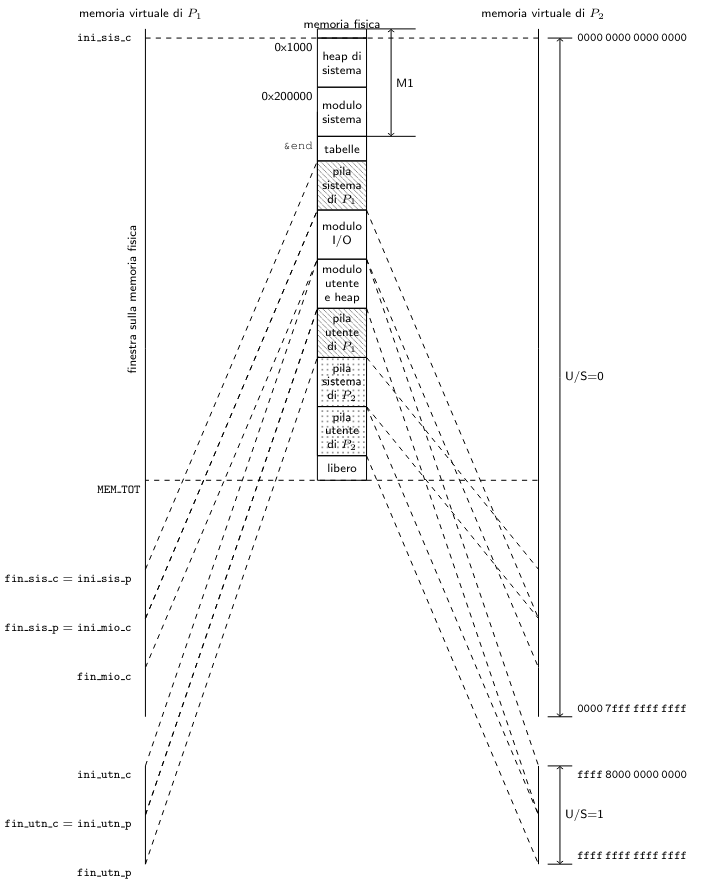
\includegraphics[scale=0.8]{../figures/mem_map.png}
\end{center}
in questo caso relativa ai trie di due processi, da cui notiamo ancora come la prima pagina non è tradotta, in quanto rappresenta l'area raggiungibile dai nullptr.
\end{minipage}

\par\bigskip

Facciamo allora alcune semplificazioni riguardo a questa struttura, in modo da avvicinarci ad un'implementazione effettiva:
\begin{itemize}
	\item Tutte le parti di livello più alte vengono create come multipli di 512 GiB, in modo che occupino intere entrate di livello 4;
	\item Le parti condivise sono \textit{"fisse"}, riferite da tabelle di livello 3 che vengono puntate nuovamente in ogni tabella di livello 4 che creiamo come radice degli alberi di traduzione di ogni processo (e che sono le stesse dell'albero di traduzione del nucleo). 
\end{itemize}

Vediamo che le tabelle di livello 3 della parte utente e sistema condivise si possono quindi creare una volta sola all'avvio del sistema (si dovrebbe ricaricare la parte codice dei processi nel caso di un sistema che carica software dal disco).
Questa allocazione viene fatta usando la \lstinline|map()| aiutata da \lstinline|alloca_frame()|, per ottenere memoria e disporre traduzioni per regioni di memoria di indirizzi prestabiliti.
Queste regioni seguono lo schema visto finora, che viene definito in codice come:
\begin{lstlisting}[language=C++, style=codestyle]	
#define I_SIS_C		0 	// prima entrata sistema/condivisa (inizio M1)
#define I_SIS_P		1		// prima entrata sistema/privata
#define I_MIO_C		2		// prima entrata modulo IO/condivisa
#define I_UTN_C   256	// prima entrata utente/condivisa (inizio M2)
#define I_UTN_P	  384	// prima entrata utente/privata

#define N_SIS_C		1		// numero entrate sistema/condivisa
#define N_SIS_P		1		// numero entrate sistema/privata
#define N_MIO_C		1		// numero entrate modulo IO/condivisa
#define N_UTN_C	  128	// numero entrate utente/convidisa
#define N_UTN_P	  128	// numero entrate utente/privata
\end{lstlisting}

Le uniche cose che vanno quindi create da zero ogni volta che si crea un processo sono la \textbf{pila sistema} in memoria sistema privata e la \textbf{pila utente} in memoria utente privata.

Avremo quindi che alla creazione di un nuovo processo dovremo creare una \textit{nuova} tabella di livello 4, che puntera alle tabelle di livello 3 delle parti condivise (memoria utente e sistema condivisa), già esistenti, e che creerà nuove tabelle di livello 3, e quindi di livello 2, ecc... per le parti private (pila utente e pila sistema).

\subsection{Creazione di processi in memoria}
Possiamo quindi vedere più nel dettaglio la creazione di processi, in particolare riguardo alla memoria e alle tabelle e traduzioni create.

\subsubsection{Albero di traduzione}
Abbiamo detto avevamo bisogno di creare nuove tabelle di livello 4 per ogni processo.
Facciamo questo come segue:
\begin{lstlisting}[language=C++, style=codestyle]	
des_proc* crea_processo(void f(natq), natq a, int prio, char liv) {
	[...]

	p->cr3 = alloca_tab(); // la nuova tabella di livello 4
	if (p->cr3 == 0)
		goto err_rel_id;
	init_root_tab(p->cr3);
	
	[...]
}
\end{lstlisting}
dove la \lstinline|init_root_tab()|, come avevamo detto, si limita a copiare le tabelle di livello 3 delle parti condivise:
\begin{lstlisting}[language=C++, style=codestyle]	
void init_root_tab(paddr dest) {
	// cr3 del processo corrente
	paddr pdir = esecuzione->cr3;

	// copia le tabelle di livello 3
	copy_des(pdir, dest, I_SIS_C, N_SIS_C);
	copy_des(pdir, dest, I_MIO_C, N_MIO_C);
	copy_des(pdir, dest, I_UTN_C, N_UTN_C);
}
\end{lstlisting}

Questa ha una duale, che semplicemente libera le entrate create:
\begin{lstlisting}[language=C++, style=codestyle]	
void clear_root_tab(paddr dest) {
	// eliminiamo le entrate create da init_root_tab()
	set_des(dest, I_SIS_C, N_SIS_C, 0);
	set_des(dest, I_MIO_C, N_MIO_C, 0);
	set_des(dest, I_UTN_C, N_UTN_C, 0);
}
\end{lstlisting}

\subsubsection{Pila}
Veniamo quindi all'inizializzazione della pila.
Questa si fa, sia per la pila utente che per la pila sistema, attraverso la \lstinline|crea_pila()|:
\begin{lstlisting}[language=C++, style=codestyle]	
bool crea_pila(paddr root_tab, vaddr bottom, natq size, natl liv)
{
	vaddr v = map(root_tab,
		bottom - size,
		bottom,
		BIT_RW | (liv == LIV_UTENTE ? BIT_US : 0),
		[](vaddr) { return alloca_frame(); });

	// caso di errore
	if (v != bottom) {
		unmap(root_tab, bottom - size, v,
			[](vaddr, paddr p, int) { rilascia_frame(p); });
		return false;
	}
	return true;
}
\end{lstlisting}
che ottiene una pila di una dimensione prestabilita allocando i frame necessari.

Questa ha ancora una duale, \lstinline|distruggi_pila()|:
\begin{lstlisting}[language=C++, style=codestyle]	
void distruggi_pila(paddr root_tab, vaddr bottom, natq size) {
	unmap(
		root_tab,
		bottom - size,
		bottom,
		[](vaddr, paddr p, int) { rilascia_frame(p); });
}
\end{lstlisting}
che si limita a liberare i frame usati.

Dal punto di vista della \lstinline|crea_processo()|, quindi, vogliamo prima inizializzare la pila sistema, e poi:
\begin{itemize}
	\item Se siamo in contesto utente:
		\begin{enumerate}
			\item Inizializzare la pila sistema;
			\item Creare la pila utente;
			\item Inizializzare la pila utente.
		\end{enumerate}
	\item Se invece siamo in contesto sistema, ci limitiamo ad inizializzare la pila sistema.
\end{itemize}

Questo in codice si traduce come:
\begin{lstlisting}[language=C++, style=codestyle]	
// creazione della pila sistema
static_assert(DIM_SYS_STACK > 0 && (DIM_SYS_STACK & 0xFFF) == 0);

// siamo in un altro processo, quindi dobbiamo accedere alla pila sistema tramite la finestra FM
pila_sistema = trasforma(p->cr3, fin_sis_p - 1) + 1;

// convertiamo a puntatore a natq, per accedervi piu' comodamente
pl = ptr_cast<natq>(pila_sistema);

if (liv == LIV_UTENTE) {
	// processo di livello utente
	// inizializzazione della pila sistema
	pl[-5] = int_cast<natq>(f);	    		// RIP (codice utente)
	pl[-4] = SEL_CODICE_UTENTE;	    		// CS (codice utente)
	pl[-3] = BIT_IF;	    	    				// RFLAGS
	pl[-2] = fin_utn_p - sizeof(natq);  // RSP
	pl[-1] = SEL_DATI_UTENTE;	    			// SS (pila utente)

	// eseguendo una IRET da questa situazione, il processo
	// passera' ad eseguire la prima istruzione della funzione f,
	// usando come pila la pila utente (al suo indirizzo virtuale)

	// creazione della pila utente
	static_assert(DIM_USR_STACK > 0 && (DIM_USR_STACK & 0xFFF) == 0);

	// inizialmente, il processo si trova a livello sistema, come
	// se avesse eseguito una istruzione INT, con la pila sistema
	// che contiene le 5 parole quadruple preparate precedentemente
	p->contesto[I_RSP] = fin_sis_p - 5 * sizeof(natq);

	p->livello = LIV_UTENTE;

	// dal momento che usiamo traduzioni diverse per le parti sistema/private
	// di tutti i processi, possiamo inizializzare p->punt_nucleo con un
	// indirizzo (virtuale) uguale per tutti i processi
	p->punt_nucleo = fin_sis_p;

	// tutti gli altri campi valgono 0
} else {
	// processo di livello sistema
	// inizializzazione della pila sistema
	pl[-6] = int_cast<natq>(f);				 // RIP (codice sistema)
	pl[-5] = SEL_CODICE_SISTEMA;  		 // CS (codice sistema)
	pl[-4] = BIT_IF;  	        			 // RFLAGS
	pl[-3] = fin_sis_p - sizeof(natq); // RSP
	pl[-2] = 0;			        					 // SS
	pl[-1] = 0;			        					 // ind. rit.

	// inizializzazione del descrittore di processo
	p->contesto[I_RSP] = fin_sis_p - 6 * sizeof(natq);

	p->livello = LIV_SISTEMA;

	// tutti gli altri campi valgono 0
}
\end{lstlisting}

\end{document}


\documentclass[a4paper,11pt]{article}
\usepackage[a4paper, margin=8em]{geometry}

% usa i pacchetti per la scrittura in italiano
\usepackage[french,italian]{babel}
\usepackage[T1]{fontenc}
\usepackage[utf8]{inputenc}
\frenchspacing 

% usa i pacchetti per la formattazione matematica
\usepackage{amsmath, amssymb, amsthm, amsfonts}

% usa altri pacchetti
\usepackage{gensymb}
\usepackage{hyperref}
\usepackage{standalone}

\usepackage{colortbl}

\usepackage{xstring}
\usepackage{karnaugh-map}

% imposta il titolo
\title{Appunti Calcolatori Elettronici}
\author{Luca Seggiani}
\date{2025}

% imposta lo stile
% usa helvetica
\usepackage[scaled]{helvet}
% usa palatino
\usepackage{palatino}
% usa un font monospazio guardabile
\usepackage{lmodern}

\renewcommand{\rmdefault}{ppl}
\renewcommand{\sfdefault}{phv}
\renewcommand{\ttdefault}{lmtt}

% circuiti
\usepackage{circuitikz}
\usetikzlibrary{babel}

% testo cerchiato
\newcommand*\circled[1]{\tikz[baseline=(char.base)]{
\node[shape=circle,draw,inner sep=2pt] (char) {#1};}}

% disponi il titolo
\makeatletter
\renewcommand{\maketitle} {
	\begin{center} 
		\begin{minipage}[t]{.8\textwidth}
			\textsf{\huge\bfseries \@title} 
		\end{minipage}%
		\begin{minipage}[t]{.2\textwidth}
			\raggedleft \vspace{-1.65em}
			\textsf{\small \@author} \vfill
			\textsf{\small \@date}
		\end{minipage}
		\par
	\end{center}

	\thispagestyle{empty}
	\pagestyle{fancy}
}
\makeatother

% disponi teoremi
\usepackage{tcolorbox}
\newtcolorbox[auto counter, number within=section]{theorem}[2][]{%
	colback=blue!10, 
	colframe=blue!40!black, 
	sharp corners=northwest,
	fonttitle=\sffamily\bfseries, 
	title=Teorema~\thetcbcounter: #2, 
	#1
}

% disponi definizioni
\newtcolorbox[auto counter, number within=section]{definition}[2][]{%
	colback=red!10,
	colframe=red!40!black,
	sharp corners=northwest,
	fonttitle=\sffamily\bfseries,
	title=Definizione~\thetcbcounter: #2,
	#1
}

% disponi codice
\usepackage{listings}
\usepackage[table]{xcolor}

\definecolor{codegreen}{rgb}{0,0.6,0}
\definecolor{codegray}{rgb}{0.5,0.5,0.5}
\definecolor{codepurple}{rgb}{0.58,0,0.82}
\definecolor{backcolour}{rgb}{0.95,0.95,0.92}

\lstdefinestyle{codestyle}{
	backgroundcolor=\color{black!5}, 
	commentstyle=\color{codegreen},
	keywordstyle=\bfseries\color{magenta},
	numberstyle=\sffamily\tiny\color{black!60},
	stringstyle=\color{green!50!black},
	basicstyle=\ttfamily\footnotesize,
	breakatwhitespace=false,         
	breaklines=true,                 
	captionpos=b,                    
	keepspaces=true,                 
	numbers=left,                    
	numbersep=5pt,                  
	showspaces=false,                
	showstringspaces=false,
	showtabs=false,                  
	tabsize=2
}

\lstdefinestyle{shellstyle}{
	backgroundcolor=\color{black!5}, 
	basicstyle=\ttfamily\footnotesize\color{black}, 
	commentstyle=\color{black}, 
	keywordstyle=\color{black},
	numberstyle=\color{black!5},
	stringstyle=\color{black}, 
	showspaces=false,
	showstringspaces=false, 
	showtabs=false, 
	tabsize=2, 
	numbers=none, 
	breaklines=true
}


\lstdefinelanguage{assembler}{ 
	keywords={AAA, AAD, AAM, AAS, ADC, ADCB, ADCW, ADCL, ADD, ADDB, ADDW, ADDL, AND, ANDB, ANDW, ANDL,
		ARPL, BOUND, BSF, BSFL, BSFW, BSR, BSRL, BSRW, BSWAP, BT, BTC, BTCB, BTCW, BTCL, BTR, 
		BTRB, BTRW, BTRL, BTS, BTSB, BTSW, BTSL, CALL, CBW, CDQ, CLC, CLD, CLI, CLTS, CMC, CMP,
		CMPB, CMPW, CMPL, CMPS, CMPSB, CMPSD, CMPSW, CMPXCHG, CMPXCHGB, CMPXCHGW, CMPXCHGL,
		CMPXCHG8B, CPUID, CWDE, DAA, DAS, DEC, DECB, DECW, DECL, DIV, DIVB, DIVW, DIVL, ENTER,
		HLT, IDIV, IDIVB, IDIVW, IDIVL, IMUL, IMULB, IMULW, IMULL, IN, INB, INW, INL, INC, INCB,
		INCW, INCL, INS, INSB, INSD, INSW, INT, INT3, INTO, INVD, INVLPG, IRET, IRETD, JA, JAE,
		JB, JBE, JC, JCXZ, JE, JECXZ, JG, JGE, JL, JLE, JMP, JNA, JNAE, JNB, JNBE, JNC, JNE, JNG,
		JNGE, JNL, JNLE, JNO, JNP, JNS, JNZ, JO, JP, JPE, JPO, JS, JZ, LAHF, LAR, LCALL, LDS,
		LEA, LEAVE, LES, LFS, LGDT, LGS, LIDT, LMSW, LOCK, LODSB, LODSD, LODSW, LOOP, LOOPE,
		LOOPNE, LSL, LSS, LTR, MOV, MOVB, MOVW, MOVL, MOVSB, MOVSD, MOVSW, MOVSX, MOVSXB,
		MOVSXW, MOVSXL, MOVZX, MOVZXB, MOVZXW, MOVZXL, MUL, MULB, MULW, MULL, NEG, NEGB, NEGW,
		NEGL, NOP, NOT, NOTB, NOTW, NOTL, OR, ORB, ORW, ORL, OUT, OUTB, OUTW, OUTL, OUTSB, OUTSD,
		OUTSW, POP, POPL, POPW, POPB, POPA, POPAD, POPF, POPFD, PUSH, PUSHL, PUSHW, PUSHB, PUSHA, 
		PUSHAD, PUSHF, PUSHFD, RCL, RCLB, RCLW, MOVSL, MOVSB, MOVSW, STOSL, STOSB, STOSW, LODSB, LODSW,
		LODSL, INSB, INSW, INSL, OUTSB, OUTSL, OUTSW
		RCLL, RCR, RCRB, RCRW, RCRL, RDMSR, RDPMC, RDTSC, REP, REPE, REPNE, RET, ROL, ROLB, ROLW,
		ROLL, ROR, RORB, RORW, RORL, SAHF, SAL, SALB, SALW, SALL, SAR, SARB, SARW, SARL, SBB,
		SBBB, SBBW, SBBL, SCASB, SCASD, SCASW, SETA, SETAE, SETB, SETBE, SETC, SETE, SETG, SETGE,
		SETL, SETLE, SETNA, SETNAE, SETNB, SETNBE, SETNC, SETNE, SETNG, SETNGE, SETNL, SETNLE,
		SETNO, SETNP, SETNS, SETNZ, SETO, SETP, SETPE, SETPO, SETS, SETZ, SGDT, SHL, SHLB, SHLW,
		SHLL, SHLD, SHR, SHRB, SHRW, SHRL, SHRD, SIDT, SLDT, SMSW, STC, STD, STI, STOSB, STOSD,
		STOSW, STR, SUB, SUBB, SUBW, SUBL, TEST, TESTB, TESTW, TESTL, VERR, VERW, WAIT, WBINVD,
	XADD, XADDB, XADDW, XADDL, XCHG, XCHGB, XCHGW, XCHGL, XLAT, XLATB, XOR, XORB, XORW, XORL},
	keywordstyle=\color{blue}\bfseries,
	ndkeywordstyle=\color{darkgray}\bfseries,
	identifierstyle=\color{black},
	sensitive=false,
	comment=[l]{\#},
	morecomment=[s]{/*}{*/},
	commentstyle=\color{purple}\ttfamily,
	stringstyle=\color{red}\ttfamily,
	morestring=[b]',
	morestring=[b]"
}

\lstset{language=assembler, style=codestyle}

% disponi sezioni
\usepackage{titlesec}

\titleformat{\section}
{\sffamily\Large\bfseries} 
{\thesection}{1em}{} 
\titleformat{\subsection}
{\sffamily\large\bfseries}   
{\thesubsection}{1em}{} 
\titleformat{\subsubsection}
{\sffamily\normalsize\bfseries} 
{\thesubsubsection}{1em}{}

% tikz
\usepackage{tikz}

% float
\usepackage{float}

% grafici
\usepackage{pgfplots}
\pgfplotsset{width=10cm,compat=1.9}

% disponi alberi
\usepackage{forest}

\forestset{
	rectstyle/.style={
		for tree={rectangle,draw,font=\large\sffamily}
	},
	roundstyle/.style={
		for tree={circle,draw,font=\large}
	}
}

% disponi algoritmi
\usepackage{algorithm}
\usepackage{algorithmic}
\makeatletter
\renewcommand{\ALG@name}{Algoritmo}
\makeatother

% disponi numeri di pagina
\usepackage{fancyhdr}
\fancyhf{} 
\fancyfoot[L]{\sffamily{\thepage}}

\makeatletter
\fancyhead[L]{\raisebox{1ex}[0pt][0pt]{\sffamily{\@title \ \@date}}} 
\fancyhead[R]{\raisebox{1ex}[0pt][0pt]{\sffamily{\@author}}}
\makeatother

\begin{document}
% sezione (data)
\section{Lezione del 08-04-25}

% stili pagina
\thispagestyle{empty}
\pagestyle{fancy}

% testo
Concluso il discorso sulla memoria virtuale, ci concentreremo nuovamente sull'hardware, nella prospettiva di approfondire l'interazione fra nucleo e dispositivi di I/O. 

\subsection{Bus PCI}
Il bus \textbf{PCI}, che sta per \textit{Peripheral Component Interconnect}, è uno standard per bus sviluppato da IBM per consentire l'espansione dei loro calcolatori attraverso schede apposite, supportando quindi una cosiddetta \textit{architettura aperta}.

Possiamo quindi immaginare che ogni scheda di espansione sia provvista dei suoi registri, delle sue interruzioni, ecc... che non devono sovrapporsi con quelli di altre schede.
Storicamente, questo rappresentava un problema, in quanto potevano crearsi \textit{conflitti} fra più schede.

Inoltre, un problema era rappresentato dai \textit{driver}, in quanto non esisteva un modo standardizzato per rilevare se una certa scheda era installata o no, e quindi se si poteva usare un certo driver.

I produttori stabilirono quindi una sorta di standard \textit{de facto}, che abbiamo già nominato: l'\textbf{ISA} (\textit{Industry Standard Architecture}).

L'idea fondamentale è che la scheda non può avere registri fissi, ma deve essere programmabile in questo dal calcolatore.
Inoltre, deve esistere una qualche modalità per rilevare le schede correntemente installate nel sistema.

Nei PC moderni sfruttiamo uno standard di derivazione dal vecchio PCI, compatibile con esso, che è il \textit{PCI Express} (e che non studieremo).

\subsubsection{Indirizzamento dei dispositivi}
Secondo lo standard PCI, separiamo il \textbf{bus locale} (quello che abbiamo visto finora) da un eventuale \textbf{albero di bus}, collegati fra di loro dai cosiddetti \textbf{ponti}.
Il \textbf{ponte ospite-PCI}, in particolare, collega il \textbf{bus principale} (il più vicino al bus locale) al bus locale, mentre questo a sua volta viene collegato ad altri bus attraverso \textbf{ponti PCI-PCI}.
Ad esempio, molti calcolatori dell'epoca erano dotati di \textit{bus ISA} collegati con appositi ponti al bus principale, per la gestione di vecchie interfacce ISA.

A ogni bus è associato un numero su 8 bit, col bus principale che si prende il numero 0.

Per indirizzare un dispositivo usiamo invece 16 bit, disposti come:
\begin{table}[H]
	\center 
	\begin{tabular} { c | c c }
		\bfseries Scopo & \bfseries Bit & \bfseries Max \\
		\hline 
		\textit{Bus} & 8 bit & 256 \\
		\textit{Device} & 5 bit & 32\\
		\textit{Function} & 3 bit & 8
	\end{tabular}
\end{table}
dove il numero di bus è lo stesso di prima.

Il numero di dispositivo differisce dal \textit{Device ID}, che vedremo fra poco, e deriva dalla posizione fisica del dispositivo nel bus.

Il numero di funzione, invece, è reso necessario da schede che implementano più funzionalità, quali ad esempio le schede grafiche moderne, che si occupano anche dell'audio.
In ogni caso, la funzione 0 deve essere implementata obbligatoriamente.

Come vediamo dalla tabella, poi, si possono avere direttamente dalle codifiche fino a 256 bus diversi, con 32 dispositivi ciascuno e 8 funzioni per dispositivo.

\subsubsection{Operazioni coi dispositivi}
Veniamo quindi a come funzionano le operazioni più semplici sul Bus PCI.
Ogni operazione sul PCI viene detta \textbf{transazione}, ed ha un \textbf{iniziatore} e un \textbf{obiettivo}, cioè il dispositivo che inizia la transazione e il dispositivo che gli risponde.

L'iniziatore delle richieste che il nostro programma invia all'I/O, notiamo, non sarà più il processore, ma il ponte ospite-PCI.
Inoltre, il bus PCI permette in verità che anche dispositivi esterni al ponte ospite-PCI facciano da iniziatori per transazioni, rendendo possibili meccanismi come il \textbf{DMA} (\textit{Direct Memory Access}). 

Sul bus vero e proprio troviamo quindi:
\begin{itemize}
	\item La linea di \textbf{clock}, che tutte le interfacce vedono, originariamente intorno ai 33 MHz.
		Sul fronte di salita del clock tutte le interfacce (idealmente) campionano i segnali sul bus;
	\item \textbf{FRAME\#}, che "incornicia" la transazione corrente: l'iniziatore lo alza quando la transazione è finita. Al massimo, a handshake avvenuto si possono avere un numero indefinito di cili di trasmissione da 4 byte: il FRAME si alza ad avvenuta trasmissione dell'ultimo fra questi;
	\item \textbf{AD}, la linea \textit{condivisa} di indirizzo o dati, a 32 bit;
	\item \textbf{C/BE\#}, \textit{controllo} e \textit{byte-enable}, codificano il tipo di operazione in fase di indirizzamento e fanno da byte-enable nel trasferimento dati;
	\item \textbf{IRDY\#} e \textbf{TRDY\#}, rispettivamente \textit{Initiator Ready} e \textit{Target Ready}, supportano l'handshake nella fase di scambio dati: l'iniziatore abbassa IRDY quando è pronto a ricevere dati o quando inizia a scriverli, mentre l'obiettivo abbassa TRDY quando inizia a inviare dati o a riceverli;
	\item \textbf{DEVSEL\#}, viene attivato dal dispositivo che riconosce, controllando C/BE e l'indirizzo su AD, una chiamata a sé stesso, quindi dal presunto \textit{obiettivo}; 
	\item \textbf{STOP\#}, viene attivato dall'\textit{obiettivo} per terminare prematuramente una transazione.
\end{itemize}
dove il \# indica \textit{attivi bassi}.

\newpage

Vediamo nel dettaglio due transazioni complete, di lettura e scrittura a 4 byte sequenziali, per capire a pieno la politica di handshake:
\begin{itemize}
	\item \textbf{Lettura:} 
	\begin{center}
		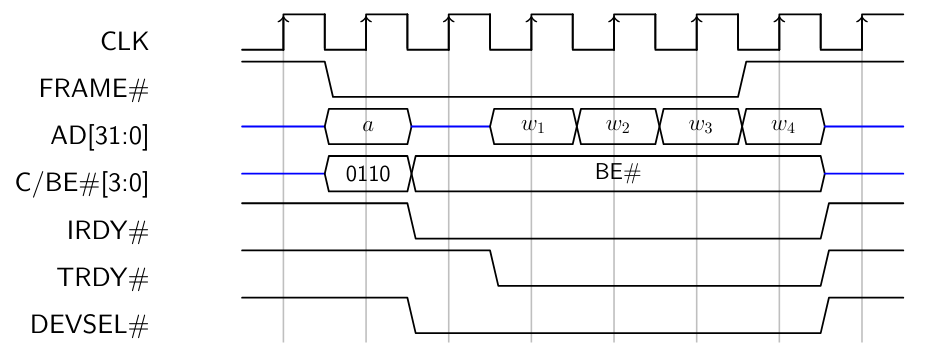
\includegraphics[scale=0.5]{../figures/pci_read.png}
	\end{center}
	Abbiamo che l'iniziatore come prima cosa porta il FRAME in basso e scrive l'indirizzo in AD e la modalità di indirizzamento in C/BE (qui \lstinline|0110|, che significa memoria).
	L'obiettivo risponde abbassando DEVSEL, al cui l'iniziatore risponde abbassando IRDY. 
	Fra l'abbassamento di IRDY e l'inizio della trasmissione (l'abbassamento di TRDY) c'è un ciclo di clock a vuoto, detto \textit{ciclo di turnaround}, che permette all'iniziatore di rilasciare AD e C/BE perchè l'obiettivo possa assumerne il controllo.
	Si trasmettono quindi 16 byte in mandate da 4, con FRAME che torna alto al quarto byte per segnalare la fine dell'operazione, e le linee di handshake (IRDY, TRDY e DEVSEL) tornano alte.

	\item \textbf{Scrittura:} 
	\begin{center}
		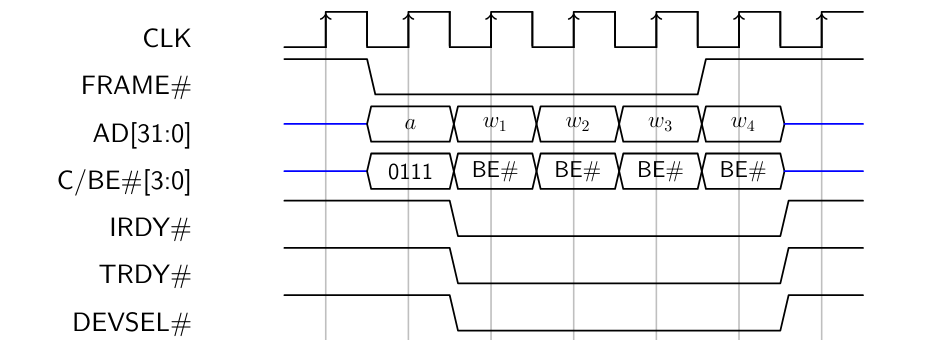
\includegraphics[scale=0.5]{../figures/pci_write.png}
	\end{center}
	Le cose si svolgono in maniera pressoché identica, con la differenza che non si necessita di un ciclo di turnaround in quanto l'iniziatore sarà l'unico a scrivere su AD e C/BE. Inoltre, possiamo immaginare che C/BE venga effettivamente modificato nel corso della scrittura, in quanto magari non vogliamo impattare tutti i byte ad ogni ciclo di scrittura.
\end{itemize}

\subsubsection{Spazio di configurazione}
Per poter lavorare con il bus PCI, poi, introduciamo un nuovo spazio indirizzabile, quello di \textbf{configurazione}.
Avremo quindi che il processore può indirizzare:
\begin{itemize}
	\item \textbf{Memoria};
	\item \textbf{I/O};
	\item \textbf{Configurazione}.
\end{itemize}
Questo spazio è rilevante solo all'avvio del calcolatore (all'esecuzione del BIOS, o come definito originariamente dallo standard, \textit{PCI BIOS}), appunto per effettuare la configurazione delle interfacce PCI installate nel sistema.
Ogni bus PCI trasporta quindi messaggi in uno qualsiasi di questi 3 spazi, e si discrimina lo spazio specifico controllando cosa l'iniziatore mette in C/BE.

Useremo lo spazio di I/O come sempre, ma i segnali del processore viaggeranno attraverso i vari ponti fino all'interfaccia desiderata.
Per quanto riguarda i dispositivi mappati in memoria (si pensi al video), invece, possiamo assumere che all'avvio il ponte ospite-PCI deve solo sapere la dimensione della memoria RAM installata, in modo da rispondere da lì in poi solo agli indirizzi \textit{di memoria} posti al di \textit{sotto} di essa.
Avevamo visto questo meccanismo nella sezione 17.2, vedendo come il bootloader ignora la zona di memoria superiore alla RAM e dedicata al bus PCI.

Notiamo che tutto questo sistema è comunque strutturato per essere trasparente al processore, e quindi invisibile lato software.

\subsubsection{Configurazione dei dispositivi}
Ogni dispositivo sul bus è obbligato a fornire, per ogni funzione e ad una certa locazione predefinita, un numero di registri che formano 64 righe da 32 bit, che devono contenere informazioni di configurazione.
I primi due dati, su 16 bit (quindi una riga), saranno il \textbf{Vendor ID} e il \textbf{Device ID}, seguiti da altri dati che non ci sono immediatamente rilevanti:

\begin{center}
	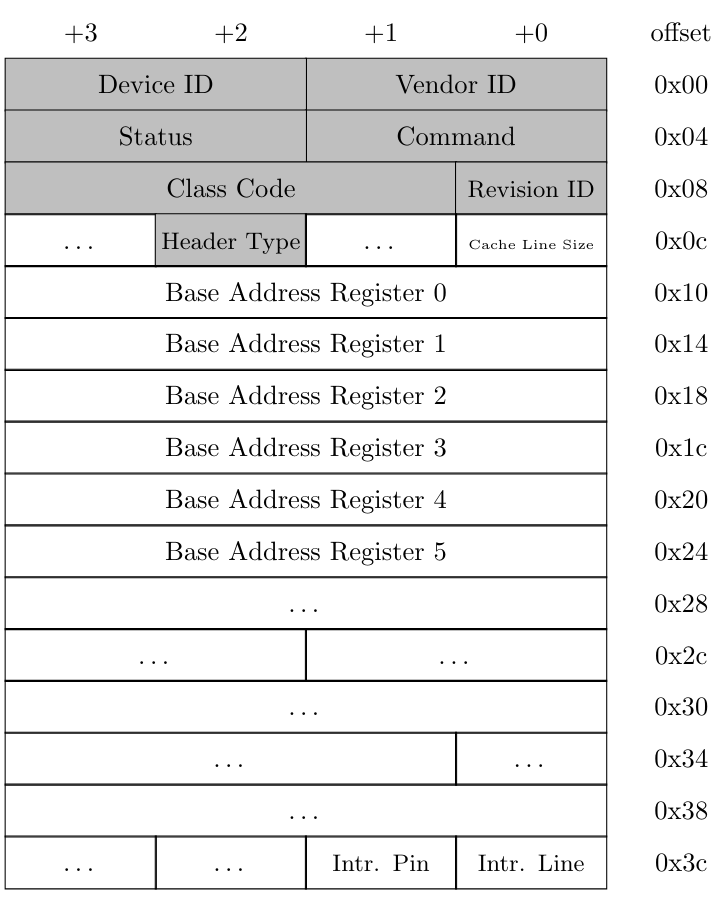
\includegraphics[scale=0.5]{../figures/config_space.png}
\end{center}

Il Vendor ID è determinato da un'autorità centrale (la \textit{PCI-SIG}): ad esempio, il vendor ID della Intel è \lstinline|0x8086|.

Per permettere quindi alla CPU di configurare i dispositivi, cioè accedere ai loro registri di configurazione, il ponte ospite-PCI rende disponibili alla CPU due registri, entrambi su 32 bit:
\begin{itemize}
	\item Il \textbf{CAP}, \textit{Configuration Address Port}, che permette di selezionare una funzione e l'offset della parola a cui si vuole accedere;
	\item Il \textbf{CDP}, \textit{Configuration Data Port}, che permette di accedere alla parola selezionata con \textit{CAP}.
\end{itemize}
Le operazioni effettuate dalla CPU attraverso questi due registri verranno trasformate automaticamente dal ponte ospite-PCI in operazioni di configurazione sui bus PCI.

La posizione di questi registri in memoria è la seguente:
\begin{table}[h!]
	\center
	\begin{tabular} { c | p{7cm} }
		\lstinline|0xcf8| & \textbf{CAP}, \textit{Configuration Address Port} \\
		\lstinline|0xcfc| & \textbf{CDP}, \textit{Configuration Data Port}	
	\end{tabular}
\end{table}

Vediamo quindi cosa deve fare il BIOS per la configurazione dei dispositivi PCI, cioè per collocarne nello spazio di I/O o in memoria eventuali registri o porzioni di memoria, rispettivamente.
Ogni dispositivo ha una \textbf{dimensione naturale} che occupa nello spazio, sia questo di memoria o di I/O.
Fornisce quindi al processore un registro, detto \textbf{BAR} (\textit{Base Address Register}), che è scrivibile solo in parte: la parte meno significativa, infatti, è fissa a 0 e determina la dimensione naturale della regione che questo occuperà.
Per rilevare la dimensione naturale, quindi, basta scrivere tutti 1 sul BAR e controllare quali bit vengono effettivamente modificati.

Il PCI BIOS dovrà quindi, attraverso i registri CAP e CDP, controllare il BAR di tutte le interfacce, determinarne la dimensione naturale e trovare una regione libera nello spazio di I/O o in memoria, a seconda del tipo di dispositivo, dove collocarle.

\subsubsection{Interruzioni PCI}
Per la gestione delle interruzioni, lo standard si ferma al dire che ogni dispositivo deve specificare per ogni funzione quale, di quattro linee di interruzione, tale funzione usa, in un apposito registro di configurazione.
Queste linee sono dette \textbf{INTA}, \textbf{INTB}, \textbf{INTC} e \textbf{INTD}, e lo spazio di configurazione della funzione contiene il dato rispetto a quale linea usa in \textit{Intr. Pin}, con 0 che significa nessuna interruzione, 1 \textit{INTA}, e così via.

\subsection{I/O nel kernel}
La maggior parte delle modifiche allo spazio di I/O apportate introducendo il bus PCI, abbiamo detto, sono effettivamente trasparenti al processore, se non per l'introduzione dei registri CAP e CDP, che devono essere comunque usati una volta sola nel PCI BIOS per la configurazione dei dispositivi.
Possiamo quindi sfruttare la maggior parte delle funzioni definite in \lstinline|libce.h| per l'input/output senza particolari problemi.

Vediamo quindi com'è implementata la gestione dell'I/O da parte del \textit{kernel}.

Avevamo detto che la motivazione principale dietro lo sviluppo del sistema multiprogrammato era che questa permetteva l'interruzione in qualsiasi momento di un \textit{processo} in esecuzione, per permettere al processore di effettuare altre operazioni.
Le interruzioni sollevate da i dispositivi esterni, vediamo, possono essere gli eventi che provocano tale cambio di contesto, e quindi la gestione del segnale in ingresso al sistema.

Ad esempio, un processo potrebbe, con la funzione \lstinline|readconsole()|, specificare un buffer e un numero di caratteri che vuole leggere da tastiera.
A questo punto, il sistema lo metterà in attesa e si occuperà di altro, riempiendo sequenzialmente il buffer via via che i tasti vengono effettivamente premuti (e quindi le relative interruzioni sollevate).
Una volta che il buffer sia riempito dal numero di caratteri richiesti dal processo, potrà quindi rimettere il processo in esecuzione, o nella lista pronti, e proseguire.

Per tenere conto di più processi che possono voler leggere contemporaneamente, poi, ci dotiamo di un semaforo che tenga conto di chi sta usando quella risorsa in un certo momento.
Un problema qui sarà come usare i semafori da lato sistema, e verrà discusso nella prossima lezione.

\end{document}


\documentclass[a4paper,11pt]{article}
\usepackage[a4paper, margin=8em]{geometry}

% usa i pacchetti per la scrittura in italiano
\usepackage[french,italian]{babel}
\usepackage[T1]{fontenc}
\usepackage[utf8]{inputenc}
\frenchspacing 

% usa i pacchetti per la formattazione matematica
\usepackage{amsmath, amssymb, amsthm, amsfonts}

% usa altri pacchetti
\usepackage{gensymb}
\usepackage{hyperref}
\usepackage{standalone}

\usepackage{colortbl}

\usepackage{xstring}
\usepackage{karnaugh-map}

% imposta il titolo
\title{Appunti Calcolatori Elettronici}
\author{Luca Seggiani}
\date{2025}

% imposta lo stile
% usa helvetica
\usepackage[scaled]{helvet}
% usa palatino
\usepackage{palatino}
% usa un font monospazio guardabile
\usepackage{lmodern}

\renewcommand{\rmdefault}{ppl}
\renewcommand{\sfdefault}{phv}
\renewcommand{\ttdefault}{lmtt}

% circuiti
\usepackage{circuitikz}
\usetikzlibrary{babel}

% testo cerchiato
\newcommand*\circled[1]{\tikz[baseline=(char.base)]{
            \node[shape=circle,draw,inner sep=2pt] (char) {#1};}}

% disponi il titolo
\makeatletter
\renewcommand{\maketitle} {
	\begin{center} 
		\begin{minipage}[t]{.8\textwidth}
			\textsf{\huge\bfseries \@title} 
		\end{minipage}%
		\begin{minipage}[t]{.2\textwidth}
			\raggedleft \vspace{-1.65em}
			\textsf{\small \@author} \vfill
			\textsf{\small \@date}
		\end{minipage}
		\par
	\end{center}

	\thispagestyle{empty}
	\pagestyle{fancy}
}
\makeatother

% disponi teoremi
\usepackage{tcolorbox}
\newtcolorbox[auto counter, number within=section]{theorem}[2][]{%
	colback=blue!10, 
	colframe=blue!40!black, 
	sharp corners=northwest,
	fonttitle=\sffamily\bfseries, 
	title=Teorema~\thetcbcounter: #2, 
	#1
}

% disponi definizioni
\newtcolorbox[auto counter, number within=section]{definition}[2][]{%
	colback=red!10,
	colframe=red!40!black,
	sharp corners=northwest,
	fonttitle=\sffamily\bfseries,
	title=Definizione~\thetcbcounter: #2,
	#1
}

% disponi codice
\usepackage{listings}
\usepackage[table]{xcolor}

\definecolor{codegreen}{rgb}{0,0.6,0}
\definecolor{codegray}{rgb}{0.5,0.5,0.5}
\definecolor{codepurple}{rgb}{0.58,0,0.82}
\definecolor{backcolour}{rgb}{0.95,0.95,0.92}

\lstdefinestyle{codestyle}{
		backgroundcolor=\color{black!5}, 
		commentstyle=\color{codegreen},
		keywordstyle=\bfseries\color{magenta},
		numberstyle=\sffamily\tiny\color{black!60},
		stringstyle=\color{green!50!black},
		basicstyle=\ttfamily\footnotesize,
		breakatwhitespace=false,         
		breaklines=true,                 
		captionpos=b,                    
		keepspaces=true,                 
		numbers=left,                    
		numbersep=5pt,                  
		showspaces=false,                
		showstringspaces=false,
		showtabs=false,                  
		tabsize=2
}

\lstdefinestyle{shellstyle}{
		backgroundcolor=\color{black!5}, 
		basicstyle=\ttfamily\footnotesize\color{black}, 
		commentstyle=\color{black}, 
		keywordstyle=\color{black},
		numberstyle=\color{black!5},
		stringstyle=\color{black}, 
		showspaces=false,
		showstringspaces=false, 
		showtabs=false, 
		tabsize=2, 
		numbers=none, 
		breaklines=true
}


\lstdefinelanguage{assembler}{ 
  keywords={AAA, AAD, AAM, AAS, ADC, ADCB, ADCW, ADCL, ADD, ADDB, ADDW, ADDL, AND, ANDB, ANDW, ANDL,
        ARPL, BOUND, BSF, BSFL, BSFW, BSR, BSRL, BSRW, BSWAP, BT, BTC, BTCB, BTCW, BTCL, BTR, 
        BTRB, BTRW, BTRL, BTS, BTSB, BTSW, BTSL, CALL, CBW, CDQ, CLC, CLD, CLI, CLTS, CMC, CMP,
        CMPB, CMPW, CMPL, CMPS, CMPSB, CMPSD, CMPSW, CMPXCHG, CMPXCHGB, CMPXCHGW, CMPXCHGL,
        CMPXCHG8B, CPUID, CWDE, DAA, DAS, DEC, DECB, DECW, DECL, DIV, DIVB, DIVW, DIVL, ENTER,
        HLT, IDIV, IDIVB, IDIVW, IDIVL, IMUL, IMULB, IMULW, IMULL, IN, INB, INW, INL, INC, INCB,
        INCW, INCL, INS, INSB, INSD, INSW, INT, INT3, INTO, INVD, INVLPG, IRET, IRETD, JA, JAE,
        JB, JBE, JC, JCXZ, JE, JECXZ, JG, JGE, JL, JLE, JMP, JNA, JNAE, JNB, JNBE, JNC, JNE, JNG,
        JNGE, JNL, JNLE, JNO, JNP, JNS, JNZ, JO, JP, JPE, JPO, JS, JZ, LAHF, LAR, LCALL, LDS,
        LEA, LEAVE, LES, LFS, LGDT, LGS, LIDT, LMSW, LOCK, LODSB, LODSD, LODSW, LOOP, LOOPE,
        LOOPNE, LSL, LSS, LTR, MOV, MOVB, MOVW, MOVL, MOVSB, MOVSD, MOVSW, MOVSX, MOVSXB,
        MOVSXW, MOVSXL, MOVZX, MOVZXB, MOVZXW, MOVZXL, MUL, MULB, MULW, MULL, NEG, NEGB, NEGW,
        NEGL, NOP, NOT, NOTB, NOTW, NOTL, OR, ORB, ORW, ORL, OUT, OUTB, OUTW, OUTL, OUTSB, OUTSD,
        OUTSW, POP, POPL, POPW, POPB, POPA, POPAD, POPF, POPFD, PUSH, PUSHL, PUSHW, PUSHB, PUSHA, 
				PUSHAD, PUSHF, PUSHFD, RCL, RCLB, RCLW, MOVSL, MOVSB, MOVSW, STOSL, STOSB, STOSW, LODSB, LODSW,
				LODSL, INSB, INSW, INSL, OUTSB, OUTSL, OUTSW
        RCLL, RCR, RCRB, RCRW, RCRL, RDMSR, RDPMC, RDTSC, REP, REPE, REPNE, RET, ROL, ROLB, ROLW,
        ROLL, ROR, RORB, RORW, RORL, SAHF, SAL, SALB, SALW, SALL, SAR, SARB, SARW, SARL, SBB,
        SBBB, SBBW, SBBL, SCASB, SCASD, SCASW, SETA, SETAE, SETB, SETBE, SETC, SETE, SETG, SETGE,
        SETL, SETLE, SETNA, SETNAE, SETNB, SETNBE, SETNC, SETNE, SETNG, SETNGE, SETNL, SETNLE,
        SETNO, SETNP, SETNS, SETNZ, SETO, SETP, SETPE, SETPO, SETS, SETZ, SGDT, SHL, SHLB, SHLW,
        SHLL, SHLD, SHR, SHRB, SHRW, SHRL, SHRD, SIDT, SLDT, SMSW, STC, STD, STI, STOSB, STOSD,
        STOSW, STR, SUB, SUBB, SUBW, SUBL, TEST, TESTB, TESTW, TESTL, VERR, VERW, WAIT, WBINVD,
        XADD, XADDB, XADDW, XADDL, XCHG, XCHGB, XCHGW, XCHGL, XLAT, XLATB, XOR, XORB, XORW, XORL},
  keywordstyle=\color{blue}\bfseries,
  ndkeywordstyle=\color{darkgray}\bfseries,
  identifierstyle=\color{black},
  sensitive=false,
  comment=[l]{\#},
  morecomment=[s]{/*}{*/},
  commentstyle=\color{purple}\ttfamily,
  stringstyle=\color{red}\ttfamily,
  morestring=[b]',
  morestring=[b]"
}

\lstset{language=assembler, style=codestyle}

% disponi sezioni
\usepackage{titlesec}

\titleformat{\section}
	{\sffamily\Large\bfseries} 
	{\thesection}{1em}{} 
\titleformat{\subsection}
	{\sffamily\large\bfseries}   
	{\thesubsection}{1em}{} 
\titleformat{\subsubsection}
	{\sffamily\normalsize\bfseries} 
	{\thesubsubsection}{1em}{}

% tikz
\usepackage{tikz}

% float
\usepackage{float}

% grafici
\usepackage{pgfplots}
\pgfplotsset{width=10cm,compat=1.9}

% disponi alberi
\usepackage{forest}

\forestset{
	rectstyle/.style={
		for tree={rectangle,draw,font=\large\sffamily}
	},
	roundstyle/.style={
		for tree={circle,draw,font=\large}
	}
}

% disponi algoritmi
\usepackage{algorithm}
\usepackage{algorithmic}
\makeatletter
\renewcommand{\ALG@name}{Algoritmo}
\makeatother

% disponi numeri di pagina
\usepackage{fancyhdr}
\fancyhf{} 
\fancyfoot[L]{\sffamily{\thepage}}

\makeatletter
\fancyhead[L]{\raisebox{1ex}[0pt][0pt]{\sffamily{\@title \ \@date}}} 
\fancyhead[R]{\raisebox{1ex}[0pt][0pt]{\sffamily{\@author}}}
\makeatother

\begin{document}
% sezione (data)
\section{Lezione del 11-04-25}

% stili pagina
\thispagestyle{empty}
\pagestyle{fancy}

% testo
Riprendiamo il discorso dell'I/O nel kernel.

\subsection{Primitive di I/O}
L'ipotesi generale è che una primitiva di I/O vuole trasferire dati da e alla memoria o da e allo spazio di I/O.
La forma generica della primitive che vorremo fornire all'utente sarà quindi del tipo:
\begin{itemize}
	\item \textbf{Lettura:}
\begin{lstlisting}[language=C++, style=codestyle]
read_n(id, char* buf, natq quanti);
\end{lstlisting}
dove prendiamo la periferica \lstinline|id|, e leggiamo \lstinline|quanti| byte nel buffer \lstinline|buf|;
	\item \textbf{Scrittura:}
\begin{lstlisting}[language=C++, style=codestyle]
write_n(id, const char* buf, natq quanti);
\end{lstlisting}
dove prendiamo la periferica \lstinline|id|, e scriviamo \lstinline|quanti| byte dal buffer \lstinline|buf|.
\end{itemize}

Avremo quindi che un certo processo $P_1$, a qualche punto della sua esecuzione, chiama una primitiva di I/O.
A questo punto il controllo passa al kernel, che si occupa quindi di gestire l'operazione, sfruttando prima di tutto le istruzioni privilegiate a cui ha accesso \lstinline|IN|, \lstinline|OUT|, ecc... e le possibilità di scheduling di cui dispone per eseguire, mentre attende per la sincronia col dispositivo, altri processi (mettendo quindi quello che aveva chiamato la primitiva in attesa).
Quando $P_1$ viene rimesso in esecuzione, non vede niente di diverso nel suo contesto privato, se non il fatto che il buffer contiene adesso l'input desiderato.

Le primitive di sistema che gestiscono un certo dispositivo prendono il nome, abbiamo detto, di \textbf{driver}.

Per realizzare il meccanismo di \textbf{sincronizzazione} sfruttiamo \textit{semaforo}: vogliamo che il processo chiami la \lstinline|sem_wait()| al momento dell'inizio dell'operazione di I/O, e che la \lstinline|sem_signal()| venga chiamata sullo stesso semaforo alla fine dell'operazione per segnalare che l'operazione è finita.

Per realizzare invece la \textbf{mutua esclusione} si sfrutta il procedimento inverso: si parte con un semaforo inizializzato a \lstinline|sem_wait()|, e successivamente ogni processo che inizia un'operazione di I/O ne prende un \textit{"gettone"}, restituendolo a termine operazione, così che nessun'altro processo possa iniziare una operazione di I/O contemporaneamente a un altro.

\subsubsection{Primitive nel kernel}
Avevamo visto che il problema era usare le \lstinline|sem_wait()| e le \lstinline|sem_signal()| lato kernel, in quanto queste effettivamente interrompono routine sistema e ne violano l'atomicità.

Vediamo però che, se ci limitiamo a non manipolare le strutture dati sistema nelle primitive \lstinline|read_n()| e \lstinline|write_n()|, non incappiamo nei rischi per cui avevamo introdotto l'atomicità delle routine sistema in primo luogo (le uniche a manipolare la lista processi saranno le \lstinline|read_n()| e \lstinline|write_n()|).

L'unico problema resterà il discorso del contesto, che verrebbe salvato così 2 volte.
Rimuoviamo allora le \lstinline|salva_stato| e \lstinline|carica_stato|.

Trasformiamo quindi le primitive di I/O in primitive effettivamente \textit{non atomiche}, che eseguono nello stesso contesto (a livello di registri) del processo chiamante.

\subsubsection{Driver}
Vediamo come si svolge la situazione lato driver.
Potremmo pensare iniziatutto di sfruttare un certo descrittore di \textit{dispositivo}, \lstinline|des_io|, realizzato ad esempio come:
\begin{lstlisting}[language=C++, style=codestyle]	
des_io {
	char* buf;
	natq quanti;

	// semafori
	natl mutex;
	natl sync;
};
\end{lstlisting}
cioè contenente tutte le informazioni necessarie al driver per soddisfare la richiesta del processo che ha richiesto l'I/O, scrivendo i dati ottenuti nel buffer \lstinline|buf| giusto all'indice \lstinline|quanti| (che incrementerà o decrementerà da solo) giusto.

Notiamo che in ogni caso il buffer rappresenta i dati lato utente, cioè come vedremo contenuti nella memoria condivisa dei processi, e nulla riguardo al dispositivo vero e proprio: i suoi dati verranno ottenuti, a controllo d'interruzione, dalla primitiva stessa attraverso i suoi procedimenti specifici.
In particolare, il buffer della \lstinline|read_n| sarà quello dove il driver dovrà scrivere cosa legge così che il processo lo veda, mentre il buffer (costante) della \lstinline|write_n| sarà quello dove il driver dovrà leggere per restituire poi al dispositivo.

La domanda è se il driver può chiamare le primitive semaforo che gestiscono i semafori di indice \lstinline|mutex| e \lstinline|sync|.
In particolare, avevamo detto che il driver avrà il compito di chiamare la \lstinline|sem_signal(sync)| per segnalare al processo che l'operazione di I/O è finita.
Abbiamo però il problema della \lstinline|salva_stato|, che andrà a sovrascrivere, quando chiamata da una routine sistema (e quindi anche da un driver) il contesto del processo in \lstinline|esecuzione| (che potrebbe essere arbitrario) con i valori correnti della routine sistema, facendo evidentemente danni. 

Potremmo allora pensare di usare direttamente la sua implementazione, cioè la \lstinline|c_sem_signal()|.
Il problema sarà che la \lstinline|c_sem_signal()| usa la \lstinline|sem_valido()| per controllare la validità del semaforo cercato, usando la \lstinline|liv_chiamante()|, che non sarebbe significativa se chiamata senza passare da un interruzione (sfrutta il CS salvato presumibilmente in pila dalla \lstinline|INT|).
Saremo quindi costretti a replicare in qualche modo la \lstinline|c_sem_signal()| nel codice del driver.

In questo modo, il codice del driver sarà effettivamente atomico.
Questo potrebbe essere problematico in quanto ci impedisce di gestire interruzioni innestate a priorità più alta.

Altre questioni di sicurezza potrebbero riguardare i cosiddetti \textbf{cavalli di Troia}: un utente potrebbe sfruttare la \lstinline|write_n()| per scrivere in locazioni di memoria arbitrarie, dove lui da solo non avrebbe potuto scrivere.
Si rende quindi necessario controllare gli indirizzi passati alle primitive di I/O lato software.
Vediamo che, a causa della grande quantità di problemi che questo controllo solleva (ad esempio, indirizzi che potrebbero fare wraparound, indirizzi virtuali non cointigui che potrebbero passare per traduzioni livello sistema, o addirittura indirizzi non tradotti che causerebbero page fault e quindi eccezioni che non possiamo gestire in routine sistema, ecc...), siamo costretti a controllare tutte le traduzioni.

Inoltre, vogliamo controllare di non accedere allo spazio di memoria privata del processo, in quanto quando il driver sarà in esecuzione questo conterrà la memoria privata del processo attualmente in esecuzione, e non del processo che ha effettivamente chiamato la primitiva.

Notiamo che questa era comunque una necessità, in quanto vogliamo che il processo passi per forza un buffer corrispondente ad un indirizzo in memoria condivisa, appunto perchè chiedere alla primitiva driver di scrivere nel suo spazio privato sarebbe complesso (a meno di non passare un indirizzo fisico, e quindi passare dalla finestra FM, cosà però abbastanza complicata dal punto di vista dei controlli).

Scriveremo quindi una funzione di controllo del buffer del genere:
\begin{lstlisting}[language=C++, style=codestyle]	
extern "C" bool c_access(vaddr begin, natq dim, bool writeable, bool shared = true)
{
	esecuzione->contesto[I_RAX] = false;

	if (!tab_iter::valid_interval(begin, dim))
		return false;

	if (shared && (!in_utn_c(begin) || (dim > 0 && !in_utn_c(begin + dim - 1))))
		return false;

	// usiamo un tab_iter per percorrere tutto il sottoalbero relativo
	// alla traduzione degli indirizzi nell'intervallo [begin, begin+dim).
	for (tab_iter it(esecuzione->cr3, begin, dim); it; it.next()) {
		tab_entry e = it.get_e();

		// interrompiamo il ciclo non appena troviamo qualcosa che non va
		if (!(e & BIT_P) || !(e & BIT_US) || (writeable && !(e & BIT_RW)))
			return false;
	}
	esecuzione->contesto[I_RAX] = true;
	return true;
}
\end{lstlisting}
che fa prima i controlli detti su intervallo e regione processi, e poi percorre l'intero albero di traduzione, controllando che ogni traduzione sia scrivibile.

\end{document}


\documentclass[a4paper,11pt]{article}
\usepackage[a4paper, margin=8em]{geometry}

% usa i pacchetti per la scrittura in italiano
\usepackage[french,italian]{babel}
\usepackage[T1]{fontenc}
\usepackage[utf8]{inputenc}
\frenchspacing 

% usa i pacchetti per la formattazione matematica
\usepackage{amsmath, amssymb, amsthm, amsfonts}

% usa altri pacchetti
\usepackage{gensymb}
\usepackage{hyperref}
\usepackage{standalone}

\usepackage{colortbl}

\usepackage{xstring}
\usepackage{karnaugh-map}

% imposta il titolo
\title{Appunti Calcolatori Elettronici}
\author{Luca Seggiani}
\date{2025}

% imposta lo stile
% usa helvetica
\usepackage[scaled]{helvet}
% usa palatino
\usepackage{palatino}
% usa un font monospazio guardabile
\usepackage{lmodern}

\renewcommand{\rmdefault}{ppl}
\renewcommand{\sfdefault}{phv}
\renewcommand{\ttdefault}{lmtt}

% circuiti
\usepackage{circuitikz}
\usetikzlibrary{babel}

% testo cerchiato
\newcommand*\circled[1]{\tikz[baseline=(char.base)]{
            \node[shape=circle,draw,inner sep=2pt] (char) {#1};}}

% disponi il titolo
\makeatletter
\renewcommand{\maketitle} {
	\begin{center} 
		\begin{minipage}[t]{.8\textwidth}
			\textsf{\huge\bfseries \@title} 
		\end{minipage}%
		\begin{minipage}[t]{.2\textwidth}
			\raggedleft \vspace{-1.65em}
			\textsf{\small \@author} \vfill
			\textsf{\small \@date}
		\end{minipage}
		\par
	\end{center}

	\thispagestyle{empty}
	\pagestyle{fancy}
}
\makeatother

% disponi teoremi
\usepackage{tcolorbox}
\newtcolorbox[auto counter, number within=section]{theorem}[2][]{%
	colback=blue!10, 
	colframe=blue!40!black, 
	sharp corners=northwest,
	fonttitle=\sffamily\bfseries, 
	title=Teorema~\thetcbcounter: #2, 
	#1
}

% disponi definizioni
\newtcolorbox[auto counter, number within=section]{definition}[2][]{%
	colback=red!10,
	colframe=red!40!black,
	sharp corners=northwest,
	fonttitle=\sffamily\bfseries,
	title=Definizione~\thetcbcounter: #2,
	#1
}

% disponi codice
\usepackage{listings}
\usepackage[table]{xcolor}

\definecolor{codegreen}{rgb}{0,0.6,0}
\definecolor{codegray}{rgb}{0.5,0.5,0.5}
\definecolor{codepurple}{rgb}{0.58,0,0.82}
\definecolor{backcolour}{rgb}{0.95,0.95,0.92}

\lstdefinestyle{codestyle}{
		backgroundcolor=\color{black!5}, 
		commentstyle=\color{codegreen},
		keywordstyle=\bfseries\color{magenta},
		numberstyle=\sffamily\tiny\color{black!60},
		stringstyle=\color{green!50!black},
		basicstyle=\ttfamily\footnotesize,
		breakatwhitespace=false,         
		breaklines=true,                 
		captionpos=b,                    
		keepspaces=true,                 
		numbers=left,                    
		numbersep=5pt,                  
		showspaces=false,                
		showstringspaces=false,
		showtabs=false,                  
		tabsize=2
}

\lstdefinestyle{shellstyle}{
		backgroundcolor=\color{black!5}, 
		basicstyle=\ttfamily\footnotesize\color{black}, 
		commentstyle=\color{black}, 
		keywordstyle=\color{black},
		numberstyle=\color{black!5},
		stringstyle=\color{black}, 
		showspaces=false,
		showstringspaces=false, 
		showtabs=false, 
		tabsize=2, 
		numbers=none, 
		breaklines=true
}


\lstdefinelanguage{assembler}{ 
  keywords={AAA, AAD, AAM, AAS, ADC, ADCB, ADCW, ADCL, ADD, ADDB, ADDW, ADDL, AND, ANDB, ANDW, ANDL,
        ARPL, BOUND, BSF, BSFL, BSFW, BSR, BSRL, BSRW, BSWAP, BT, BTC, BTCB, BTCW, BTCL, BTR, 
        BTRB, BTRW, BTRL, BTS, BTSB, BTSW, BTSL, CALL, CBW, CDQ, CLC, CLD, CLI, CLTS, CMC, CMP,
        CMPB, CMPW, CMPL, CMPS, CMPSB, CMPSD, CMPSW, CMPXCHG, CMPXCHGB, CMPXCHGW, CMPXCHGL,
        CMPXCHG8B, CPUID, CWDE, DAA, DAS, DEC, DECB, DECW, DECL, DIV, DIVB, DIVW, DIVL, ENTER,
        HLT, IDIV, IDIVB, IDIVW, IDIVL, IMUL, IMULB, IMULW, IMULL, IN, INB, INW, INL, INC, INCB,
        INCW, INCL, INS, INSB, INSD, INSW, INT, INT3, INTO, INVD, INVLPG, IRET, IRETD, JA, JAE,
        JB, JBE, JC, JCXZ, JE, JECXZ, JG, JGE, JL, JLE, JMP, JNA, JNAE, JNB, JNBE, JNC, JNE, JNG,
        JNGE, JNL, JNLE, JNO, JNP, JNS, JNZ, JO, JP, JPE, JPO, JS, JZ, LAHF, LAR, LCALL, LDS,
        LEA, LEAVE, LES, LFS, LGDT, LGS, LIDT, LMSW, LOCK, LODSB, LODSD, LODSW, LOOP, LOOPE,
        LOOPNE, LSL, LSS, LTR, MOV, MOVB, MOVW, MOVL, MOVSB, MOVSD, MOVSW, MOVSX, MOVSXB,
        MOVSXW, MOVSXL, MOVZX, MOVZXB, MOVZXW, MOVZXL, MUL, MULB, MULW, MULL, NEG, NEGB, NEGW,
        NEGL, NOP, NOT, NOTB, NOTW, NOTL, OR, ORB, ORW, ORL, OUT, OUTB, OUTW, OUTL, OUTSB, OUTSD,
        OUTSW, POP, POPL, POPW, POPB, POPA, POPAD, POPF, POPFD, PUSH, PUSHL, PUSHW, PUSHB, PUSHA, 
				PUSHAD, PUSHF, PUSHFD, RCL, RCLB, RCLW, MOVSL, MOVSB, MOVSW, STOSL, STOSB, STOSW, LODSB, LODSW,
				LODSL, INSB, INSW, INSL, OUTSB, OUTSL, OUTSW
        RCLL, RCR, RCRB, RCRW, RCRL, RDMSR, RDPMC, RDTSC, REP, REPE, REPNE, RET, ROL, ROLB, ROLW,
        ROLL, ROR, RORB, RORW, RORL, SAHF, SAL, SALB, SALW, SALL, SAR, SARB, SARW, SARL, SBB,
        SBBB, SBBW, SBBL, SCASB, SCASD, SCASW, SETA, SETAE, SETB, SETBE, SETC, SETE, SETG, SETGE,
        SETL, SETLE, SETNA, SETNAE, SETNB, SETNBE, SETNC, SETNE, SETNG, SETNGE, SETNL, SETNLE,
        SETNO, SETNP, SETNS, SETNZ, SETO, SETP, SETPE, SETPO, SETS, SETZ, SGDT, SHL, SHLB, SHLW,
        SHLL, SHLD, SHR, SHRB, SHRW, SHRL, SHRD, SIDT, SLDT, SMSW, STC, STD, STI, STOSB, STOSD,
        STOSW, STR, SUB, SUBB, SUBW, SUBL, TEST, TESTB, TESTW, TESTL, VERR, VERW, WAIT, WBINVD,
        XADD, XADDB, XADDW, XADDL, XCHG, XCHGB, XCHGW, XCHGL, XLAT, XLATB, XOR, XORB, XORW, XORL},
  keywordstyle=\color{blue}\bfseries,
  ndkeywordstyle=\color{darkgray}\bfseries,
  identifierstyle=\color{black},
  sensitive=false,
  comment=[l]{\#},
  morecomment=[s]{/*}{*/},
  commentstyle=\color{purple}\ttfamily,
  stringstyle=\color{red}\ttfamily,
  morestring=[b]',
  morestring=[b]"
}

\lstset{language=assembler, style=codestyle}

% disponi sezioni
\usepackage{titlesec}

\titleformat{\section}
	{\sffamily\Large\bfseries} 
	{\thesection}{1em}{} 
\titleformat{\subsection}
	{\sffamily\large\bfseries}   
	{\thesubsection}{1em}{} 
\titleformat{\subsubsection}
	{\sffamily\normalsize\bfseries} 
	{\thesubsubsection}{1em}{}

% tikz
\usepackage{tikz}

% float
\usepackage{float}

% grafici
\usepackage{pgfplots}
\pgfplotsset{width=10cm,compat=1.9}

% disponi alberi
\usepackage{forest}

\forestset{
	rectstyle/.style={
		for tree={rectangle,draw,font=\large\sffamily}
	},
	roundstyle/.style={
		for tree={circle,draw,font=\large}
	}
}

% disponi algoritmi
\usepackage{algorithm}
\usepackage{algorithmic}
\makeatletter
\renewcommand{\ALG@name}{Algoritmo}
\makeatother

% disponi numeri di pagina
\usepackage{fancyhdr}
\fancyhf{} 
\fancyfoot[L]{\sffamily{\thepage}}

\makeatletter
\fancyhead[L]{\raisebox{1ex}[0pt][0pt]{\sffamily{\@title \ \@date}}} 
\fancyhead[R]{\raisebox{1ex}[0pt][0pt]{\sffamily{\@author}}}
\makeatother

\begin{document}
% sezione (data)
\section{Lezione del 15-04-25}

% stili pagina
\thispagestyle{empty}
\pagestyle{fancy}

% testo
\subsection{Gestione di primitive di I/O quasi atomiche nel kernel reale}
Abbiamo che quanto abbiamo visto finora sulle primitive di I/O non corrisponde propriamente al kernel reale: avevamo infatti il problema di dover realizzare primitive \textit{"quasi"} atomiche, nel senso che potevano essere interrotte
dalle primitive semaforiche (che usavano per sincronizzazione e mutua esclusione), ma avevano anche accesso alle strutture dati sistema (in particolare le code processi), per cui bisogna fare attenzione nella loro implementazione di non toccare parti sensibili, in modo da evitare errori di difficile rilevazione.

Possiamo migliorare leggermente questa architettura separando il \textbf{modulo} sistema (inteso come un insieme di file compilati e collegati insieme) dal modulo di I/O, cioè stabilendo la seguente distinzione:
\begin{itemize}
	\item \textbf{Modulo sistema}, implementato in \lstinline|sistema.cpp| e \lstinline|sistema.s| (parti C++ e assembler);
	\item \textbf{Modulo di I/O}, implementato in \lstinline|io.cpp| e \lstinline|io.s| (come sopra).
\end{itemize}

Avremo quindi che la parte I/O dipenderà dalla parte sistema, ma non avrà accesso a tutte le sue struttura dati: ad esempio non avra accesso alle code processi.
Si andrà quindi a creare la seguente struttura:

\begin{center}
	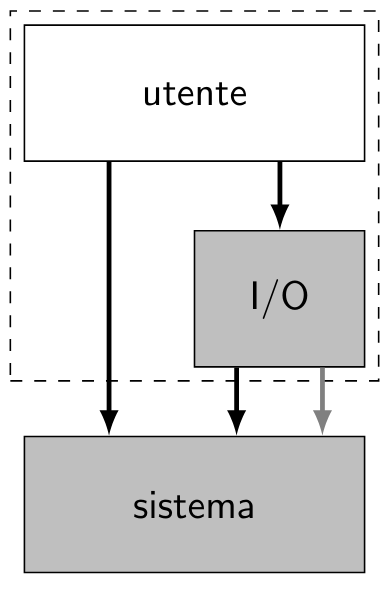
\includegraphics[scale=0.35]{../figures/moduli_sys_io.png}
\end{center}
dove le frecce nere indicano primitive accessibili a livello utente e le frecce grigie indicano primitive accessibili a livello sistema.

Prima di capire il perché di questa distinzione vediamo di capire a quale livello lavora il modulo di I/O.

Abbiamo visto in 8.1.1 come il registro CS ci permette di definire 4 livelli, o \textit{ring}, e di come storicamente i ring intermedi (1 e 2) venivano usati per i driver (quindi, per i nostri scopi, i moduli di I/O):
\begin{table}[H]
	\center \rowcolors{2}{white}{black!10}
	\begin{tabular} { c | c | c }
		\bfseries CS & \bfseries Ring & \bfseries Tipo \\
		\hline 
		00 & Ring 0 & Kernel (sistema) \\
		01 & Ring 1 & Driver  \textit{(non più supportato)}\\
		10 & Ring 2 &  / / \\
		11 & Ring 3 & Utente \\
	\end{tabular}
\end{table}
Oggi, però, questa distinzione non esiste più (assieme alla memoria segmentata, si perde anche questa funzionalità del registro CS), e gli unici livelli permessi sono 0 (che abbiamo assunto come livello sistema) e 3 (che abbiamo assunto come livello utente).

Dovremo quindi porre il modulo di I/O in livello sistema, in modo che questo possa avere accesso alle funzioni privilegiate di cui vogliamo privare l'utente.
L'unico vantaggio dell'architettura adottata sarà quindi quello di impedire al modulo di I/O di intaccare le strutture dati sensbili lato sistema.
Ad esempio, non si potranno nemmeno usare erroneamente le \lstinline|salva_stato()| o \lstinline|carica_stato()| nelle primtive di I/O, in quanto queste non saranno nemmeno definite nel modulo di I/O.

\subsubsection{Processi esterni}
Avremo quindi che i driver saranno rappresentati da processi, detti \textbf{processi esterni}: le primitivi accessibili solo da livello sistema dal modulo di I/O saranno appunto le primitive per la creazione di processi esterni (la \lstinline|activate_pe()|), e altre primitive utili al modulo di I/O (a cui l'utente non dovrà avere accesso).
Queste saranno
Il sistema avrà quindi il compito di definire, su richiesta del modulo di I/O \textbf{handler} caricati nella IDT, che si occuperanno di gestire le interruzioni esterne semplicemente indirizzandole ai processi di I/O relativi, creati anch'essi dal modulo di I/O.

\end{document}


\documentclass[a4paper,11pt]{article}
\usepackage[a4paper, margin=8em]{geometry}

% usa i pacchetti per la scrittura in italiano
\usepackage[french,italian]{babel}
\usepackage[T1]{fontenc}
\usepackage[utf8]{inputenc}
\frenchspacing 

% usa i pacchetti per la formattazione matematica
\usepackage{amsmath, amssymb, amsthm, amsfonts}

% usa altri pacchetti
\usepackage{gensymb}
\usepackage{hyperref}
\usepackage{standalone}

\usepackage{colortbl}

\usepackage{xstring}
\usepackage{karnaugh-map}

% imposta il titolo
\title{Appunti Calcolatori Elettronici}
\author{Luca Seggiani}
\date{2025}

% imposta lo stile
% usa helvetica
\usepackage[scaled]{helvet}
% usa palatino
\usepackage{palatino}
% usa un font monospazio guardabile
\usepackage{lmodern}

\renewcommand{\rmdefault}{ppl}
\renewcommand{\sfdefault}{phv}
\renewcommand{\ttdefault}{lmtt}

% circuiti
\usepackage{circuitikz}
\usetikzlibrary{babel}

% testo cerchiato
\newcommand*\circled[1]{\tikz[baseline=(char.base)]{
            \node[shape=circle,draw,inner sep=2pt] (char) {#1};}}

% disponi il titolo
\makeatletter
\renewcommand{\maketitle} {
	\begin{center} 
		\begin{minipage}[t]{.8\textwidth}
			\textsf{\huge\bfseries \@title} 
		\end{minipage}%
		\begin{minipage}[t]{.2\textwidth}
			\raggedleft \vspace{-1.65em}
			\textsf{\small \@author} \vfill
			\textsf{\small \@date}
		\end{minipage}
		\par
	\end{center}

	\thispagestyle{empty}
	\pagestyle{fancy}
}
\makeatother

% disponi teoremi
\usepackage{tcolorbox}
\newtcolorbox[auto counter, number within=section]{theorem}[2][]{%
	colback=blue!10, 
	colframe=blue!40!black, 
	sharp corners=northwest,
	fonttitle=\sffamily\bfseries, 
	title=Teorema~\thetcbcounter: #2, 
	#1
}

% disponi definizioni
\newtcolorbox[auto counter, number within=section]{definition}[2][]{%
	colback=red!10,
	colframe=red!40!black,
	sharp corners=northwest,
	fonttitle=\sffamily\bfseries,
	title=Definizione~\thetcbcounter: #2,
	#1
}

% disponi codice
\usepackage{listings}
\usepackage[table]{xcolor}

\definecolor{codegreen}{rgb}{0,0.6,0}
\definecolor{codegray}{rgb}{0.5,0.5,0.5}
\definecolor{codepurple}{rgb}{0.58,0,0.82}
\definecolor{backcolour}{rgb}{0.95,0.95,0.92}

\lstdefinestyle{codestyle}{
		backgroundcolor=\color{black!5}, 
		commentstyle=\color{codegreen},
		keywordstyle=\bfseries\color{magenta},
		numberstyle=\sffamily\tiny\color{black!60},
		stringstyle=\color{green!50!black},
		basicstyle=\ttfamily\footnotesize,
		breakatwhitespace=false,         
		breaklines=true,                 
		captionpos=b,                    
		keepspaces=true,                 
		numbers=left,                    
		numbersep=5pt,                  
		showspaces=false,                
		showstringspaces=false,
		showtabs=false,                  
		tabsize=2
}

\lstdefinestyle{shellstyle}{
		backgroundcolor=\color{black!5}, 
		basicstyle=\ttfamily\footnotesize\color{black}, 
		commentstyle=\color{black}, 
		keywordstyle=\color{black},
		numberstyle=\color{black!5},
		stringstyle=\color{black}, 
		showspaces=false,
		showstringspaces=false, 
		showtabs=false, 
		tabsize=2, 
		numbers=none, 
		breaklines=true
}


\lstdefinelanguage{assembler}{ 
  keywords={AAA, AAD, AAM, AAS, ADC, ADCB, ADCW, ADCL, ADD, ADDB, ADDW, ADDL, AND, ANDB, ANDW, ANDL,
        ARPL, BOUND, BSF, BSFL, BSFW, BSR, BSRL, BSRW, BSWAP, BT, BTC, BTCB, BTCW, BTCL, BTR, 
        BTRB, BTRW, BTRL, BTS, BTSB, BTSW, BTSL, CALL, CBW, CDQ, CLC, CLD, CLI, CLTS, CMC, CMP,
        CMPB, CMPW, CMPL, CMPS, CMPSB, CMPSD, CMPSW, CMPXCHG, CMPXCHGB, CMPXCHGW, CMPXCHGL,
        CMPXCHG8B, CPUID, CWDE, DAA, DAS, DEC, DECB, DECW, DECL, DIV, DIVB, DIVW, DIVL, ENTER,
        HLT, IDIV, IDIVB, IDIVW, IDIVL, IMUL, IMULB, IMULW, IMULL, IN, INB, INW, INL, INC, INCB,
        INCW, INCL, INS, INSB, INSD, INSW, INT, INT3, INTO, INVD, INVLPG, IRET, IRETD, JA, JAE,
        JB, JBE, JC, JCXZ, JE, JECXZ, JG, JGE, JL, JLE, JMP, JNA, JNAE, JNB, JNBE, JNC, JNE, JNG,
        JNGE, JNL, JNLE, JNO, JNP, JNS, JNZ, JO, JP, JPE, JPO, JS, JZ, LAHF, LAR, LCALL, LDS,
        LEA, LEAVE, LES, LFS, LGDT, LGS, LIDT, LMSW, LOCK, LODSB, LODSD, LODSW, LOOP, LOOPE,
        LOOPNE, LSL, LSS, LTR, MOV, MOVB, MOVW, MOVL, MOVSB, MOVSD, MOVSW, MOVSX, MOVSXB,
        MOVSXW, MOVSXL, MOVZX, MOVZXB, MOVZXW, MOVZXL, MUL, MULB, MULW, MULL, NEG, NEGB, NEGW,
        NEGL, NOP, NOT, NOTB, NOTW, NOTL, OR, ORB, ORW, ORL, OUT, OUTB, OUTW, OUTL, OUTSB, OUTSD,
        OUTSW, POP, POPL, POPW, POPB, POPA, POPAD, POPF, POPFD, PUSH, PUSHL, PUSHW, PUSHB, PUSHA, 
				PUSHAD, PUSHF, PUSHFD, RCL, RCLB, RCLW, MOVSL, MOVSB, MOVSW, STOSL, STOSB, STOSW, LODSB, LODSW,
				LODSL, INSB, INSW, INSL, OUTSB, OUTSL, OUTSW
        RCLL, RCR, RCRB, RCRW, RCRL, RDMSR, RDPMC, RDTSC, REP, REPE, REPNE, RET, ROL, ROLB, ROLW,
        ROLL, ROR, RORB, RORW, RORL, SAHF, SAL, SALB, SALW, SALL, SAR, SARB, SARW, SARL, SBB,
        SBBB, SBBW, SBBL, SCASB, SCASD, SCASW, SETA, SETAE, SETB, SETBE, SETC, SETE, SETG, SETGE,
        SETL, SETLE, SETNA, SETNAE, SETNB, SETNBE, SETNC, SETNE, SETNG, SETNGE, SETNL, SETNLE,
        SETNO, SETNP, SETNS, SETNZ, SETO, SETP, SETPE, SETPO, SETS, SETZ, SGDT, SHL, SHLB, SHLW,
        SHLL, SHLD, SHR, SHRB, SHRW, SHRL, SHRD, SIDT, SLDT, SMSW, STC, STD, STI, STOSB, STOSD,
        STOSW, STR, SUB, SUBB, SUBW, SUBL, TEST, TESTB, TESTW, TESTL, VERR, VERW, WAIT, WBINVD,
        XADD, XADDB, XADDW, XADDL, XCHG, XCHGB, XCHGW, XCHGL, XLAT, XLATB, XOR, XORB, XORW, XORL},
  keywordstyle=\color{blue}\bfseries,
  ndkeywordstyle=\color{darkgray}\bfseries,
  identifierstyle=\color{black},
  sensitive=false,
  comment=[l]{\#},
  morecomment=[s]{/*}{*/},
  commentstyle=\color{purple}\ttfamily,
  stringstyle=\color{red}\ttfamily,
  morestring=[b]',
  morestring=[b]"
}

\lstset{language=assembler, style=codestyle}

% disponi sezioni
\usepackage{titlesec}

\titleformat{\section}
	{\sffamily\Large\bfseries} 
	{\thesection}{1em}{} 
\titleformat{\subsection}
	{\sffamily\large\bfseries}   
	{\thesubsection}{1em}{} 
\titleformat{\subsubsection}
	{\sffamily\normalsize\bfseries} 
	{\thesubsubsection}{1em}{}

% tikz
\usepackage{tikz}

% float
\usepackage{float}

% grafici
\usepackage{pgfplots}
\pgfplotsset{width=10cm,compat=1.9}

% disponi alberi
\usepackage{forest}

\forestset{
	rectstyle/.style={
		for tree={rectangle,draw,font=\large\sffamily}
	},
	roundstyle/.style={
		for tree={circle,draw,font=\large}
	}
}

% disponi algoritmi
\usepackage{algorithm}
\usepackage{algorithmic}
\makeatletter
\renewcommand{\ALG@name}{Algoritmo}
\makeatother

% disponi numeri di pagina
\usepackage{fancyhdr}
\fancyhf{} 
\fancyfoot[L]{\sffamily{\thepage}}

\makeatletter
\fancyhead[L]{\raisebox{1ex}[0pt][0pt]{\sffamily{\@title \ \@date}}} 
\fancyhead[R]{\raisebox{1ex}[0pt][0pt]{\sffamily{\@author}}}
\makeatother

\begin{document}
% sezione (data)
\section{Lezione del 15-04-25}

% stili pagina
\thispagestyle{empty}
\pagestyle{fancy}

% testo
Avevamo quindi visto come si era introdotto un nuovo modulo, il modulo di I/O, che aveva il compito di gestire da gestire l'I/O da livello sistema, fornendo primitive di I/O e processi (driver) al modulo utente e sfruttando primitive, sia accessibili a livello utente che accessibili a livello sistema (quindi solo a lui) del sistema.

\subsubsection{Cambi di contesto a processi esterni}
Avremo quindi che in un dato momento sulla macchina sono in esecuzione i processi utente ($P_1$, $P_2$, ecc...) e i processi \textit{esterni} di I/O.
Assumiamo per adesso di avere un solo processo di I/O, chiamato appunto $IO$.

Nel momento in cui uno dei processi utente (diciamo $P_1$) chiama una primitiva di I/O, come ad esempio la \lstinline|read_n()| già nominata, viene messo in attesa e si mettono in esecuzione altri processi.
Di qui in poi, all'arrivo di un'interruzione esterna relativa all'operazione di I/O corrente, viene eseguito l'handler (definito in sistema) e quindi da questo messo in esecuzione il processo $IO$, che riempie ad ogni chiamata il buffer, e all'ultima chiamata rimette in lista pronti (attraverso i meccanismi implementati coi semafori visti in 19.1.5) il processo $P_1$.

\subsubsection{Implementazione degli handler}
Un'idea di base potrebbe essere quella di dedicare un \textit{processo esterno} ad ogni tipo di interruzione esterna nell'IDT.
Abbiamo visto come l'APIC supporta 24 piedini di interruzione esterna (\lstinline|IREQ|), il cui tipo di interruzione nell'IDT può essere scelto via software modificando appositi registri.
Vorremo quindi creare l'associazione:
$$
\text{piedino di interruzione} \rightarrow \text{processo esterno}
$$
cioè all'arrivo dell'interruzione esterna, il processore deve eseguire l'handler corretto come definito nella IDT, e questa deve mettere in esecuzione il processo corrente.

Servira quindi anche un \textit{handler} per ogni tipo di interruzione esterna, corrispondente al suo processo esterno (definiremo quindi \lstinline|handler_0|, \lstinline|handler_1|, ..., \lstinline|handler_23|).

La struttura di un handler generico sarà la seguente:
\begin{lstlisting}	
handler_i:
	# gestiamo l'interruzione
	call salva_stato

	# sospensdiamo il processo in esecuzione
	call inspronti

	# trova il processo esterno corrispondente
	mov a_p+i*8, %rax
	# e mettilo in esecuzione
	movq %rax, esecuzione

	call carica_stato
	iretq
\end{lstlisting}

\lstinline|a_p| conterrà l'indirizzo della prima entrata di una lista di puntatori ai descrittori dei processi esterni:
\begin{center}
	\begin{tabular}{ p{.4cm} c }
& \lstinline|a_p|
\end{tabular}

\begin{tabular}{c |c|}
	0 & Processo esterno 0 \\ 
	$\vdots$ & // \\ 
	23 & Processo esterno 23
\end{tabular}
\end{center}

Questa si definisce nel sistema come:
\begin{lstlisting}[language=C++, style=codestyle]	
// MAX_IRQ e' il numero di linee di interruzione (24)
des_proc* a_p[apic::MAX_IRQ];
\end{lstlisting}

\subsubsection{Implementazione dei processi esterni}
I processi esterni avranno quindi struttura simile.
Di base, avremo bisogno (come abbiamo visto) di descrittori associati a periferiche che tengono conto dei tipi specifici alle periferiche, e delle informazioni riguardanti l'ultima richiesta di I/O:
\begin{lstlisting}[language=C++, style=codestyle]	
des_io array_des_io[MAX_DES_IO];
\end{lstlisting}

Avremo quindi che un processo esterno è implementato come:
\begin{lstlisting}[language=C++, style=codestyle]	
void estern_i(natq id) {
	des_io *d = &array_des_io[id];
	// non servono controlli, id e' fidato

	// i processi esterni non terminano mai, quindi facciamo un ciclo infinito
	for(;;) {
		// qui si gestisce l'interruzione
		// ...
		
		// aspetta prossima interruzione
		wfi();
	}
}
\end{lstlisting}

Notiamo che chiaramente non possiamo chiamare, finita la gestione, \lstinline|schedulatore()|, in quanto questo processo (non atomico) non deve avere accesso a strutture dati sensibili, e proprio per questo è stato messo nel modulo di I/O.

Si rende quindi disponibile un'altra di quelle primitive non accessibili all'utente, cioè la \lstinline|wfi()| (\textit{Wait For Interrupt}), che appunto sospende il processo mettendolo in attesa fino alla prossima interruzione di sua competenza, e mettendo in esecuzione un altro processo (cioè facendo la chiamata a \lstinline|schedulatore()| che volevamo fare in primo luogo).

Possiamo vedere l'implementazione, in assembler, della \lstinline|wfi()|:
\begin{lstlisting}	
a_wfi:
	call salva_stato
	
	# intanto rispondiamo all'APIC
	call apic_send_EOI

	# non dobbiamo fare niente col processo esterno, 
	# e' gia' nella tabella a_p
	
	call schedulatore

	call carica_stato
	iretq
\end{lstlisting}

Vediamo quindi il dettaglio di poter usare, questa volta, le primitive semaforiche all'interno del processo esterno (in quanto il processo deve essere interrompibile), cioè dire:
\begin{lstlisting}[language=C++, style=codestyle]	
extern "C" void estern_i(natq id)
{
	des_io *d = &array_des_io[id];
	// non servono controlli, id e' fidato

	for (;;) {
		// gestisci l'interruzione

		if (d->quanti == 0) {
			sem_signal(ce->sync); // qui puoi usare la sem_signal()
		}

		wfi(); // ecco la wfi() per il ritorno
	}
}
\end{lstlisting}

Infine, vediamo a scopo di esempio il processo esterno per una periferica nota, la \textit{CE} del 19.1.5:
\begin{lstlisting}[language=C++, style=codestyle]	
extern "C" void estern_ce(natq id)
{
	// trova il descrittore
	des_ce *ce = &array_ce[id];

	for (;;) {
		// gestisci l'interruzione
		ce->quanti--;
		if (ce->quanti == 0) {
			outputb(0, ce->iCTL);
		}
		char b = inputb(ce->iRBR);
		*ce->buf = b;
		ce->buf++;

		if (ce->quanti == 0) {
			sem_signal(ce->sync); // qui puoi usare la sem_signal()
		}

		wfi(); // ecco la wfi() per il ritorno
	}
}
\end{lstlisting}

Tastiera e hard disk dispongono di processi esterni simili, definiti rispettivamente in \lstinline|estern_kbd()| e \lstinline|estern_hd()|.

Vediamo un dettaglio: durante l'esecuzione di un processo esterno, non potrà accadere che questo viene interrotto da un interruzione esterna relativa allo stesso processo: questo perchè le interruzioni esterne relative a quel dispositivo sono effettivamente disattivate fino alla chiamata di \lstinline|wfi()|, cioè quando viene chiamata la \lstinline|apic_send_EOI()| (e non si può interrompere la \lstinline|wfi()| perchè è una primitiva di sistema, quindi atomica).

Esiste invece la possibilità che un interruzione di livello più alto nella IDT vada ad interrompere il processo esterno (quindi si metta in esecuzione il processo esterno relativo a \textit{quella} interruzione), ma questo è desiderabile in quanto corrisponde in maniera naturale alla priorità di gestione delle interruzioni esterne secondo l'APIC.

\subsubsection{Creazione di processi esterni}
Vediamo quindi nel dettaglio la \lstinline|activate_pe()|, di uso concesso solo al modulo di I/O, che viene usata per creare i processi esterni.
Questa sarà diversa dalla comune \lstinline|activate_p()|, in quanto dovrà anche impostare la tabella \lstinline|a_p| per gli handler.

La funzione avrà quindi firma: \lstinline|activate_pe(void (*f)(natq), natq id, natl prio, nat livello, natb irq)|, cioè si specifica:
\begin{itemize}
	\item La \textbf{funzione} (\lstinline|f|) che realizza il processo stesso;
	\item L'\textbf{indice} (\lstinline|id|) di processo;
	\item La \textbf{priorità} (\lstinline|prio|) del processo (che per i processi determinerà anche il tipo di interruzione nell'IDT);
	\item Il \textbf{livello} (\lstinline|livello|) del processo, fin qui tutto normale;
	\item La \textbf{linea di interruzione} (\lstinline|IRQ|) che tale processo esterno gestisce.
\end{itemize}

Come anticipato, un discorso importante va fatto sulla priorità di questi processi.
Abbiamo infatti la priorità \textit{da noi} definita, cioè \lstinline|prio|, e la priorità nell'APIC (quindi nella IDT), data dal codice di interruzione assegnato ad una linea \lstinline|IRQ|.
Questa seconda priorità, che chiamiamo \textbf{tipo}, viene ricavata direttamente dalla proprietà \lstinline|prio| secondo la seguente formula:
$$
\text{\lstinline|prio|} = \text{\lstinline|MAX_PRIO_UTENTE|} + \text{\lstinline|tipo|}
$$

Da qui in poi, le parti di creazione vera e propria del processo potranno essere messe in comune con la \lstinline|activate_p()|, e la \lstinline|activate_pe()| avrà il solo compito aggiuntivo di predisporre un handler, con relativo setup dell'APIC e caricamento dell'handler nell'IDT.

\subsubsection{Implementazione del modulo I/O}
Vediamo quindi la struttura generaled del modulo I/O stesso.
Questo dispone delle sue primitive, che definisce per l'utente e carica nella IDT attraverso la primitiva sistema \lstinline|fill_gate()| (potrebbe farlo da sé, in quanto gira a livello utente, ma non lo fa per \textit{"educazione"} nei confronti del modulo sistema, cioè si centralizza la gestione dell'IDT per evitare errori).

Le primitive definite gestiscono quindi essenzialmente tastiera, video ed hard disk, cioè si dispone delle primitive:
\begin{lstlisting}[language=assembler, style=codestyle]	
# inserimento delle primitive di I/O nell'IDT
fill_io_gate	IO_TIPO_HDR			a_readhd_n
fill_io_gate	IO_TIPO_HDW			a_writehd_n
fill_io_gate	IO_TIPO_DMAHDR	a_dmareadhd_n
fill_io_gate	IO_TIPO_DMAHDW	a_dmawritehd_n
fill_io_gate	IO_TIPO_RCON		a_readconsole
fill_io_gate	IO_TIPO_WCON		a_writeconsole
fill_io_gate	IO_TIPO_INIC		a_iniconsole
fill_io_gate	IO_TIPO_GMI			a_getiomeminfo
\end{lstlisting}

I processi esterni per le periferiche (tastiera e hard disk) sono quindi definiti come nel paragrafo precedente, cioè si ha:
\begin{lstlisting}[language=C++, style=codestyle]	
// processo esterno associato alla tastiera
void estern_kbd(natq) {
	// ...
}

// processo esterno per le richieste di interruzione dell'hard disk
void estern_hd(natq) {
	// ...
}
\end{lstlisting}

\subsubsection{Inizializzazione del modulo I/O}
Possiamo quindi vedere un ulteriore dettaglio riguardo alla sequenza di boot, cioè quella che riguarda l'inizializzazione dell'I/O.

Avremo infatti nel \lstinline|main()| del modulo sistema la seguente chiamata all'entry point del modulo I/O:
\begin{lstlisting}[language=C++, style=codestyle]	
extern "C" void main(natq) {
	flog(LOG_INFO, "Creo il processo main I/O");
	main_io = crea_processo(mio_entry, int_cast<natq>(&io_init_done), MAX_EXT_PRIO, LIV_SISTEMA);
	if (main_io == nullptr) {
		flog(LOG_ERR, "impossibile creare il processo main I/O");
		goto error;
	}
	processi++;
	flog(LOG_INFO, "Attendo inizializzazione modulo I/O...");

	// cediamo il controllo al modulo I/O e aspettiamo che setti
	// la variable io_init_done
	cedi_controllo(main_io);

	// sostanzialmente una sorta di sem_wait()
	while (!io_init_done) 
		halt();	// abilita temporaneamente le interruzioni esterne
}
\end{lstlisting}
dove la funzione \lstinline|cedi_controllo()| ha il compito di salvare lo stato corrente del kernel in pila in modo che vi si possa ritornare dopo l'esecuzione del \textit{processo di inizializzazione} (è proprio un processo) di un altro modulo.

A questo punto il modulo di I/O prenderà il controllo dal suo entry point:
\begin{lstlisting}[language=C++, style=codestyle]	
extern "C" void main_io(natq p)
{
	// questo e' il flag che sta guardando il main() di sistema
	int *p_io_init_done = ptr_cast<int>(p);

	// riempi la IDT delle primitive di I/O
	fill_io_gates();

	// inizializza l'heap
	ioheap_mutex = sem_ini(1);
	if (ioheap_mutex == 0xFFFFFFFF) {
		flog(LOG_ERR, "impossible creare semaforo ioheap_mutex");
		abort_p();
	}
	char* end_ = allinea_ptr(_end, DIM_PAGINA);
	heap_init(end_, DIM_IO_HEAP);
	flog(LOG_INFO, "Heap del modulo I/O: %llxB [%p, %p)", DIM_IO_HEAP,
			end_, end_ + DIM_IO_HEAP);

	// inizializza la console (tastiera + video)
	flog(LOG_INFO, "Inizializzo la console (kbd + vid)");
	if (!console_init()) {
		flog(LOG_ERR, "inizializzazione console fallita");
		abort_p();
	}

	// inizializza l'hard disk
	flog(LOG_INFO, "Inizializzo la gestione dell'hard disk");
	if (!hd_init()) {
		flog(LOG_ERR, "inizializzazione hard disk fallita");
		abort_p();
	}

	// avverti main che hai finito
	*p_io_init_done = 1;

	// termina
	terminate_p();
}
\end{lstlisting}

Abbiamo quindi una serie di funzioni (\lstinline|heap_init()|, \lstinline|console_init()|, \lstinline|hd_init()|, ...) che hanno il compito di inizializzare ogni dispositivo.
Queste, oltre ad inizializzare tutte le informazioni relative al descrittore di dispositivo, hanno il compito di creare il processo esterno di gestione di tale dispositivo.

Ad esempio, riguardo alle periferiche di tipo \textit{CE} descritte in 19.1.5 (e ammesso quindi di avere più periferiche dello stesso tipo nel bus), potremmo definire la funzione di inizializzazione:
\begin{lstlisting}[language=C++, style=codestyle]	
// trova le periferiche CE installate e crea i rispettivi processi esterni
bool ce_init()
{
	// scansiona il bus PCI per le periferiche di tipo CE
	for (natb bus = 0, dev = 0, fun = 0;
	     pci::find_dev(bus, dev, fun, 0xedce, 0x1234);
	     pci::next(bus, dev, fun))
	{
		if (next_ce >= MAX_CE) {
			flog(LOG_WARN, "troppi dispositivi ce");
			break;
		}

		// crea il descrittore
		des_ce *ce = &array_ce[next_ce];

		// configuralo
		ioaddr base = pci::read_confl(bus, dev, fun, 0x10);
		base &= ~0x1;
		ce->iCTL = base;
		ce->iSTS = base + 4;
		ce->iRBR = base + 8;

		if ( (ce->sync = sem_ini(0)) == 0xFFFFFFFF ) {
			flog(LOG_WARN, "ce%d: impossibile allocare semaforo sync", next_ce);
			break;
		}
		if ( (ce->mutex = sem_ini(1)) == 0xFFFFFFFF ) {
			flog(LOG_WARN, "ce%d: impossibile allocare semaforo mutex", next_ce);
			break;
		}

		// trova la linea di interruzione del dispositivo
		natb irq = pci::read_confb(bus, dev, fun, 0x3c);

		// attiva il procsso esterno
		if (activate_pe(estern_ce, next_ce, MIN_EXT_PRIO + 0x80, LIV_SISTEMA, irq) == 0xFFFFFFFF) {
			flog(LOG_WARN, "ce%d: impossibile attivare processo esterno", next_ce);
			break;
		}
		// log...

		next_ce++;
	}

	// restituisci true se non sei riuscito ad inizializzare
	return next_ce != 0;
}
\end{lstlisting}

Implementazioni simili si trovano per la \lstinline|console_init()|, che chiama a sua volta \lstinline|vid_init()| e \lstinline|kbd_init()|, e la \lstinline|hd_init()|.

Come ultimo dettaglio, ricordiamo che il timer è comunque gestito da sistema, utilizzando i driver come definiti in \lstinline|19.1.5| (in particolare, \lstinline|driver_td()|). 

\end{document}


\documentclass[a4paper,11pt]{article}
\usepackage[a4paper, margin=8em]{geometry}

% usa i pacchetti per la scrittura in italiano
\usepackage[french,italian]{babel}
\usepackage[T1]{fontenc}
\usepackage[utf8]{inputenc}
\frenchspacing 

% usa i pacchetti per la formattazione matematica
\usepackage{amsmath, amssymb, amsthm, amsfonts}

% usa altri pacchetti
\usepackage{gensymb}
\usepackage{hyperref}
\usepackage{standalone}

\usepackage{colortbl}

\usepackage{xstring}
\usepackage{karnaugh-map}

% imposta il titolo
\title{Appunti Calcolatori Elettronici}
\author{Luca Seggiani}
\date{2025}

% imposta lo stile
% usa helvetica
\usepackage[scaled]{helvet}
% usa palatino
\usepackage{palatino}
% usa un font monospazio guardabile
\usepackage{lmodern}

\renewcommand{\rmdefault}{ppl}
\renewcommand{\sfdefault}{phv}
\renewcommand{\ttdefault}{lmtt}

% circuiti
\usepackage{circuitikz}
\usetikzlibrary{babel}

% testo cerchiato
\newcommand*\circled[1]{\tikz[baseline=(char.base)]{
\node[shape=circle,draw,inner sep=2pt] (char) {#1};}}

% disponi il titolo
\makeatletter
\renewcommand{\maketitle} {
	\begin{center} 
		\begin{minipage}[t]{.8\textwidth}
			\textsf{\huge\bfseries \@title} 
		\end{minipage}%
		\begin{minipage}[t]{.2\textwidth}
			\raggedleft \vspace{-1.65em}
			\textsf{\small \@author} \vfill
			\textsf{\small \@date}
		\end{minipage}
		\par
	\end{center}

	\thispagestyle{empty}
	\pagestyle{fancy}
}
\makeatother

% disponi teoremi
\usepackage{tcolorbox}
\newtcolorbox[auto counter, number within=section]{theorem}[2][]{%
	colback=blue!10, 
	colframe=blue!40!black, 
	sharp corners=northwest,
	fonttitle=\sffamily\bfseries, 
	title=Teorema~\thetcbcounter: #2, 
	#1
}

% disponi definizioni
\newtcolorbox[auto counter, number within=section]{definition}[2][]{%
	colback=red!10,
	colframe=red!40!black,
	sharp corners=northwest,
	fonttitle=\sffamily\bfseries,
	title=Definizione~\thetcbcounter: #2,
	#1
}

% disponi codice
\usepackage{listings}
\usepackage[table]{xcolor}

\definecolor{codegreen}{rgb}{0,0.6,0}
\definecolor{codegray}{rgb}{0.5,0.5,0.5}
\definecolor{codepurple}{rgb}{0.58,0,0.82}
\definecolor{backcolour}{rgb}{0.95,0.95,0.92}

\lstdefinestyle{codestyle}{
	backgroundcolor=\color{black!5}, 
	commentstyle=\color{codegreen},
	keywordstyle=\bfseries\color{magenta},
	numberstyle=\sffamily\tiny\color{black!60},
	stringstyle=\color{green!50!black},
	basicstyle=\ttfamily\footnotesize,
	breakatwhitespace=false,         
	breaklines=true,                 
	captionpos=b,                    
	keepspaces=true,                 
	numbers=left,                    
	numbersep=5pt,                  
	showspaces=false,                
	showstringspaces=false,
	showtabs=false,                  
	tabsize=2
}

\lstdefinestyle{shellstyle}{
	backgroundcolor=\color{black!5}, 
	basicstyle=\ttfamily\footnotesize\color{black}, 
	commentstyle=\color{black}, 
	keywordstyle=\color{black},
	numberstyle=\color{black!5},
	stringstyle=\color{black}, 
	showspaces=false,
	showstringspaces=false, 
	showtabs=false, 
	tabsize=2, 
	numbers=none, 
	breaklines=true
}


\lstdefinelanguage{assembler}{ 
	keywords={AAA, AAD, AAM, AAS, ADC, ADCB, ADCW, ADCL, ADD, ADDB, ADDW, ADDL, AND, ANDB, ANDW, ANDL,
		ARPL, BOUND, BSF, BSFL, BSFW, BSR, BSRL, BSRW, BSWAP, BT, BTC, BTCB, BTCW, BTCL, BTR, 
		BTRB, BTRW, BTRL, BTS, BTSB, BTSW, BTSL, CALL, CBW, CDQ, CLC, CLD, CLI, CLTS, CMC, CMP,
		CMPB, CMPW, CMPL, CMPS, CMPSB, CMPSD, CMPSW, CMPXCHG, CMPXCHGB, CMPXCHGW, CMPXCHGL,
		CMPXCHG8B, CPUID, CWDE, DAA, DAS, DEC, DECB, DECW, DECL, DIV, DIVB, DIVW, DIVL, ENTER,
		HLT, IDIV, IDIVB, IDIVW, IDIVL, IMUL, IMULB, IMULW, IMULL, IN, INB, INW, INL, INC, INCB,
		INCW, INCL, INS, INSB, INSD, INSW, INT, INT3, INTO, INVD, INVLPG, IRET, IRETD, JA, JAE,
		JB, JBE, JC, JCXZ, JE, JECXZ, JG, JGE, JL, JLE, JMP, JNA, JNAE, JNB, JNBE, JNC, JNE, JNG,
		JNGE, JNL, JNLE, JNO, JNP, JNS, JNZ, JO, JP, JPE, JPO, JS, JZ, LAHF, LAR, LCALL, LDS,
		LEA, LEAVE, LES, LFS, LGDT, LGS, LIDT, LMSW, LOCK, LODSB, LODSD, LODSW, LOOP, LOOPE,
		LOOPNE, LSL, LSS, LTR, MOV, MOVB, MOVW, MOVL, MOVSB, MOVSD, MOVSW, MOVSX, MOVSXB,
		MOVSXW, MOVSXL, MOVZX, MOVZXB, MOVZXW, MOVZXL, MUL, MULB, MULW, MULL, NEG, NEGB, NEGW,
		NEGL, NOP, NOT, NOTB, NOTW, NOTL, OR, ORB, ORW, ORL, OUT, OUTB, OUTW, OUTL, OUTSB, OUTSD,
		OUTSW, POP, POPL, POPW, POPB, POPA, POPAD, POPF, POPFD, PUSH, PUSHL, PUSHW, PUSHB, PUSHA, 
		PUSHAD, PUSHF, PUSHFD, RCL, RCLB, RCLW, MOVSL, MOVSB, MOVSW, STOSL, STOSB, STOSW, LODSB, LODSW,
		LODSL, INSB, INSW, INSL, OUTSB, OUTSL, OUTSW
		RCLL, RCR, RCRB, RCRW, RCRL, RDMSR, RDPMC, RDTSC, REP, REPE, REPNE, RET, ROL, ROLB, ROLW,
		ROLL, ROR, RORB, RORW, RORL, SAHF, SAL, SALB, SALW, SALL, SAR, SARB, SARW, SARL, SBB,
		SBBB, SBBW, SBBL, SCASB, SCASD, SCASW, SETA, SETAE, SETB, SETBE, SETC, SETE, SETG, SETGE,
		SETL, SETLE, SETNA, SETNAE, SETNB, SETNBE, SETNC, SETNE, SETNG, SETNGE, SETNL, SETNLE,
		SETNO, SETNP, SETNS, SETNZ, SETO, SETP, SETPE, SETPO, SETS, SETZ, SGDT, SHL, SHLB, SHLW,
		SHLL, SHLD, SHR, SHRB, SHRW, SHRL, SHRD, SIDT, SLDT, SMSW, STC, STD, STI, STOSB, STOSD,
		STOSW, STR, SUB, SUBB, SUBW, SUBL, TEST, TESTB, TESTW, TESTL, VERR, VERW, WAIT, WBINVD,
	XADD, XADDB, XADDW, XADDL, XCHG, XCHGB, XCHGW, XCHGL, XLAT, XLATB, XOR, XORB, XORW, XORL},
	keywordstyle=\color{blue}\bfseries,
	ndkeywordstyle=\color{darkgray}\bfseries,
	identifierstyle=\color{black},
	sensitive=false,
	comment=[l]{\#},
	morecomment=[s]{/*}{*/},
	commentstyle=\color{purple}\ttfamily,
	stringstyle=\color{red}\ttfamily,
	morestring=[b]',
	morestring=[b]"
}

\lstset{language=assembler, style=codestyle}

% disponi sezioni
\usepackage{titlesec}

\titleformat{\section}
{\sffamily\Large\bfseries} 
{\thesection}{1em}{} 
\titleformat{\subsection}
{\sffamily\large\bfseries}   
{\thesubsection}{1em}{} 
\titleformat{\subsubsection}
{\sffamily\normalsize\bfseries} 
{\thesubsubsection}{1em}{}

% tikz
\usepackage{tikz}

% float
\usepackage{float}

% grafici
\usepackage{pgfplots}
\pgfplotsset{width=10cm,compat=1.9}

% disponi alberi
\usepackage{forest}

\forestset{
	rectstyle/.style={
		for tree={rectangle,draw,font=\large\sffamily}
	},
	roundstyle/.style={
		for tree={circle,draw,font=\large}
	}
}

% disponi algoritmi
\usepackage{algorithm}
\usepackage{algorithmic}
\makeatletter
\renewcommand{\ALG@name}{Algoritmo}
\makeatother

% disponi numeri di pagina
\usepackage{fancyhdr}
\fancyhf{} 
\fancyfoot[L]{\sffamily{\thepage}}

\makeatletter
\fancyhead[L]{\raisebox{1ex}[0pt][0pt]{\sffamily{\@title \ \@date}}} 
\fancyhead[R]{\raisebox{1ex}[0pt][0pt]{\sffamily{\@author}}}
\makeatother

\begin{document}
% sezione (data)
\section{Lezione del 28-04-25}

% stili pagina
\thispagestyle{empty}
\pagestyle{fancy}

% testo
\subsection{DMA}
Vediamo di introdurre il meccanismo del \textbf{DMA} (\textit{Direct Memory Access}).

Finora l'accesso a periferiche era fatto a \textit{controllo programma} o \textit{controllo interruzione}.
Chiaramente il controllo programma era più veloce, in quanto il programma provvedeva a trasferire ogni byte immediatamente appena l'interfaccia era pronta, mentre nel controllo interruzione bisognava prima eseguire tutti i passaggi necessari all'esecuzione degli \textit{handler} per portare in esecuzione il processo esterno, ecc... 

Introduciamo quindi il DMA per delegare tutta l'operazione di trasferimento dati dalle interfacce alle interfacce stesse.
Vorremo quindi avere delle primitive:
\begin{itemize}
	\item \lstinline|read_n|, trasferimento da interfaccia a RAM di un buffer $[b, b + n)$;
	\item \lstinline|write_n|, trasferimento da RAM a interfaccia di un buffer $[b, b+n)$.
\end{itemize}

Se è l'interfaccia stessa a compiere l'operazione di trasferimento, al processore servirà nuovamente un modo di controllare l'esito dell'operazione, che potra essere ancora a \textit{controllo programma} o a \textit{controllo interruzione} (che è il caso più comune).

Aggiungiamo quindi un \textbf{controllore DMA} al bus visto finora.
Questo sarà di base dotato di due registri, uno per il buffer corrente (\textbf{B}) e uno per la sua dimensione (\textbf{N}), e potrà accedere in lettura e scrittura allo spazio di memoria al pari di come farebbe la CPU.
Notiamo che non c'è bisogno che la RAM distingua fra operazioni CP o DMA, in quanto per questa sono equivalenti.

Dotiamo quindi il controllore DMA di due linee di handshake \lstinline|HOLD| e \lstinline|HOLDA|. 
Al momento dell'inizio di un'operazione DMA, il controllore alza \lstinline|HOLD|, e la CPU risponde con \lstinline|HOLDA|.
Da qui in poi il controllore lavora sul bus, in regime di \lstinline|cycle-stealing|, cioè "rubando" cicli di accesso alla CPU.
Finita l'operazione, il controllore abbassa nuovamente \lstinline|HOLD|, a cui la CPU risponde abbassando \lstinline|HOLDA| e riprendendo a scrivere sul bus.

Storicamente questo meccanismo era utile per interfacce più veloci della CPU stessa (così era la RAM, ed erano ad esempio i controllori video, che si dividevano circa la metà del tempo RAM).
Oggi, lo stesso discorso vale ad esempio per interfacce di rete, che raggiungono velocità del Gigabit al secondo.

\subsubsection{DMA e cache}
Vediamo di reintrodurre nel bus così modificato la cache.
Innanzitutto, i contendenti al bus non saranno più CPU e controllore DMA, ma cache e controllore BUS, per cui le linee di \lstinline|HOLD| e \lstinline|HOLDA| saranno fra questi due.

Il vantaggio immediato che abbiamo è che probabilmente la maggior parte dei dati necessari alla CPU saranno in cache, per cui il regime di cycle-stealing non sarà troppo dannoso all'attività della CPU (ricordiamo che la cache accede al bus solamente quando si ha una \textit{miss}).

Un problema potrebbe invece essere che la cache potrebbe perdersi gli aggiornamenti effettuati dal controllore DMA.

\par\smallskip
\noindent
\textbf{\sffamily{Write-through}} \\
Supponiamo ad esempio che la cache adotti una politica \textit{write-through}, e che chiaramente il programmatore si impegni a non toccare il buffer per tutto il tempo del trasferimento.

\begin{itemize}
	\item 
		In questo caso, per operazioni di scrittura su dispositivo non ci saranno problemi, in quanto la politicha write-trough mantiene sia la RAM che la cache in uno stato identico e consistente, e il controllore DMA non modifica la RAM in operazioni di uscita.
	\item
		Viceversa, per operazioni di lettura da dispositivo avremo problemi, in quanto potremmo intaccare una zona di memoria che era replicata in cache, e la cache non avrà modo di conoscere tale aggiornamento.

		Per ovviare a tale problema abbiamo effettivamente due soluzioni:
		\begin{itemize}
			\item La prima soluzione è \textit{lato hardware}, e consiste nel dotare la cache della possibilità di fare \textit{snooping} del bus, cioè capire a quali indirizzi il DMA sta accedendo, farne un lookup esattamente nella maniera in cui si farebbe lookup degli indirizzi richiesti dalla CPU, e procedere ricopiando i dati modificati (\textit{snarfing}) o direttamente invalidando tale porzione di cache (soluzione adottata dall'architettura Intel x86);
			\item La seconda soluzione è \textit{lato software}, e consiste nel dotare il controllore di cache di un'apposita istruzione per l'invalidazione di cache.
				Utilizzeremo quindi questa istruzione per invalidare i buffer forniti per la lettura da dispositivo al DMA, idealmente alla fine dell'operazione di trasferimento.

				Nel frattempo chiaramente non vorremmo toccare nessuna delle cacheline impegnate dal buffer, che possono definire una regione anche maggiore in dimensioni del buffer stesso.
				L'invalidazione a termine operazione viene effettuata a fine operazione proprio per questo motivo, ma una soluzione alternativa potrebbe anche essere l'adottare buffer allineati ai 64 KiB delle cacheline.
		\end{itemize}
\end{itemize}

\par\smallskip
\noindent
\textbf{\sffamily{Write-back}} \\
Fatta l'ipotesi di \textit{write-trough}, cioè di scritture effettuate in differita dalla cache, che mantiene le modifiche temporaneamente nella sua memoria, avremo problemi sia in lettura che in scrittura.

\begin{itemize}
	\item 
		In scrittura su dispositivo avremo chiaramente che il buffer in RAM potrebbe non essere stato aggiornato con le modifiche in RAM al momento dell'inizio dell'operazione da parte del controllore DMA.
		\begin{itemize}
			\item Qui la soluzione \textit{lato hardware} è di definire un protocollo per cui il controllore DMA deve prima parlare con la cache, fornendo l'indirizzo a cui intende accedere (questa fase viene detta sempre di \textit{snooping}).
				In questo caso la cache ha il tempo di controllare l'indirizzo e quindi capire se la cacheline corrispondente è \textit{dirty}, e quindi in RAM ce n'è una versione obsoleta.
				A questo punto potrà agire di conseguenza, fornendo lei stessa i dati aggiornati o effettuando una write-back;
			\item La soluzione \textit{lato software} sarà invece di fornire un'istruzione di pulizia, che permetta di forzare il write-back delle cacheline coinvolte nel buffer prima di iniziare l'operazione di lettura in RAM da parte del controllore DMA.
		\end{itemize}
	\item
		In lettura da dispositivo avremo invece che il controllore DMA potrebbe intaccare zone di memoria per cui la cache stava pianificando scritture in differita.
	\begin{itemize}
		\item In questo caso il chipset PIIX3 emulato da QEMU, ad esempio, ottiene dalla cache la versione più aggiornata (se questa esiste in cache), effettua il merge internamente al controllore DMA, che provvede poi ad effettuare la scrittura in RAM;
		Per cacheline complete, abbiamo che il DMA può adottare anche il protocollo \textit{write invalidate}, per cui la cache attraverso un'operazione di snooping può verificare che un intera cacheline è stata modificata ed invalidarla;
	\item La stessa istruzione di pulizia di cui abbiamo parlato nel caso precedente vale anche per risolvere questo problema \textit{lato software}, sempre prima dell'operazione di trasferimento (in modo che la versione dei dati in RAMsia la più recente, cioè quella ottenuta dal controllore DMA).
\end{itemize}
\end{itemize}

\subsubsection{DMA e MMU}
Reintroduciamo infine la MMU.
Qui il problema sarà chiaramente che la CPU conoscerà indirizzi virtuali, mentre la DMU avrà bisogno di indirizzi fisici.

Far passare la DMU attraverso la MMU non sarà una soluzione, in quanto non possiamo essere sicuri che durante l'operazione di trasferimento l'albero di traduzione resta lo stesso.

Abbiamo quindi che il problema dovrà essere risolto lato software, passando al controllore DMA direttamente indirizzi fisici, attraverso la finestra FM.
A questo punto però non potremmo aspettarci il corretto trasferimento di regioni di memoria di dimensione superiore a quella di una pagina, in quanto il controllore DMA non ha modo di capire quando passare da una pagina all'altra, o dove queste pagine siano in primo luogo.

Vogliamo quindi che i buffer che passiamo al controllore DMA non superino i confini di una pagina, e saremo quindi costretti a segmentare buffer che passano per più confini.

\par\smallskip

Infine, vorremo che il kernel si impegni a mantenere costante l'impiego dei buffer forniti al controllore DMA, cioè non effettui swap in o swap out dei processi che li forniscono mentre l'operazione di trasferimento è ancora in corso, in quanto il controllore non ha modo di rilevare tali variazioni.

\subsubsection{DMA nel bus PCI}
Inseriamo quindi il controllore DMA nel bus PCI.

In questo caso sarà il ponte ospite-PCI ad occuparsi del DMA.

Avremo quindi bisogno che nei singoli bus PCI ogni interfaccia abbia la possibilità di prendere il controllo del bus, secondo il cosiddetto \textbf{bus mastering}.
Il bus mastering nei bus PCI viene gestito da un \textbf{arbitro}, che è collegato con linee \lstinline|REQ| e \lstinline|ACK| ad ogni interfaccia.
Le interfacce richiedono quindi accesso al bus attraverso la \lstinline|REQ|, mentre questo gli risponde attraverso la \lstinline|ACK|.

Le operazioni potranno essere poi \textit{bufferizzate} dal ponte ospite-PCI, cioè questo potrà memorizzare le modifiche in RAM ottenute lato bus PCI, per poi riportarle in differita alla RAM vera e propria.

Questo potrebbe dare dei problemi per quanto riguarda la sincronizzazione fra interfacce e CPU, in quanto un'interfaccia potrebbe inviare un segnale di termine operazione attraverso l'APIC, quando essa \textit{crede} l'operazione sia finita (e lo farà perche lato bus PCI questa effettivamente lo è), mentre lato bus locale il ponte non ha ancora attualizzato i dati in RAM.
\begin{itemize}
	\item La soluzione \textit{lato hardware} sarà quella di collegare l'APIC al ponte, in modo da poter ritardare le interruzioni esterne alla fine delle operazioni di trasferimento.

		Possiamo anticipare che nei processori moderni gli interrupt si inviano attraverso scritture in regioni specifiche di memoria, che l'apparato CPU riconosce autonomamente come interruzione.
		Questo corrisponde in un delay naturale fra i trasferimenti e l'invio di interruzioni da una stessa interfaccia.

\end{itemize}

Notiamo che entrambe le soluzioni richiedono che il ponte adotti una politica FIFO alla gestione dei trasferimenti.

\end{document}


\documentclass[a4paper,11pt]{article}
\usepackage[a4paper, margin=8em]{geometry}

% usa i pacchetti per la scrittura in italiano
\usepackage[french,italian]{babel}
\usepackage[T1]{fontenc}
\usepackage[utf8]{inputenc}
\frenchspacing 

% usa i pacchetti per la formattazione matematica
\usepackage{amsmath, amssymb, amsthm, amsfonts}

% usa altri pacchetti
\usepackage{gensymb}
\usepackage{hyperref}
\usepackage{standalone}

\usepackage{colortbl}

\usepackage{xstring}
\usepackage{karnaugh-map}

% imposta il titolo
\title{Appunti Calcolatori Elettronici}
\author{Luca Seggiani}
\date{2025}

% imposta lo stile
% usa helvetica
\usepackage[scaled]{helvet}
% usa palatino
\usepackage{palatino}
% usa un font monospazio guardabile
\usepackage{lmodern}

\renewcommand{\rmdefault}{ppl}
\renewcommand{\sfdefault}{phv}
\renewcommand{\ttdefault}{lmtt}

% circuiti
\usepackage{circuitikz}
\usetikzlibrary{babel}

% testo cerchiato
\newcommand*\circled[1]{\tikz[baseline=(char.base)]{
            \node[shape=circle,draw,inner sep=2pt] (char) {#1};}}

% disponi il titolo
\makeatletter
\renewcommand{\maketitle} {
	\begin{center} 
		\begin{minipage}[t]{.8\textwidth}
			\textsf{\huge\bfseries \@title} 
		\end{minipage}%
		\begin{minipage}[t]{.2\textwidth}
			\raggedleft \vspace{-1.65em}
			\textsf{\small \@author} \vfill
			\textsf{\small \@date}
		\end{minipage}
		\par
	\end{center}

	\thispagestyle{empty}
	\pagestyle{fancy}
}
\makeatother

% disponi teoremi
\usepackage{tcolorbox}
\newtcolorbox[auto counter, number within=section]{theorem}[2][]{%
	colback=blue!10, 
	colframe=blue!40!black, 
	sharp corners=northwest,
	fonttitle=\sffamily\bfseries, 
	title=Teorema~\thetcbcounter: #2, 
	#1
}

% disponi definizioni
\newtcolorbox[auto counter, number within=section]{definition}[2][]{%
	colback=red!10,
	colframe=red!40!black,
	sharp corners=northwest,
	fonttitle=\sffamily\bfseries,
	title=Definizione~\thetcbcounter: #2,
	#1
}

% disponi codice
\usepackage{listings}
\usepackage[table]{xcolor}

\definecolor{codegreen}{rgb}{0,0.6,0}
\definecolor{codegray}{rgb}{0.5,0.5,0.5}
\definecolor{codepurple}{rgb}{0.58,0,0.82}
\definecolor{backcolour}{rgb}{0.95,0.95,0.92}

\lstdefinestyle{codestyle}{
		backgroundcolor=\color{black!5}, 
		commentstyle=\color{codegreen},
		keywordstyle=\bfseries\color{magenta},
		numberstyle=\sffamily\tiny\color{black!60},
		stringstyle=\color{green!50!black},
		basicstyle=\ttfamily\footnotesize,
		breakatwhitespace=false,         
		breaklines=true,                 
		captionpos=b,                    
		keepspaces=true,                 
		numbers=left,                    
		numbersep=5pt,                  
		showspaces=false,                
		showstringspaces=false,
		showtabs=false,                  
		tabsize=2
}

\lstdefinestyle{shellstyle}{
		backgroundcolor=\color{black!5}, 
		basicstyle=\ttfamily\footnotesize\color{black}, 
		commentstyle=\color{black}, 
		keywordstyle=\color{black},
		numberstyle=\color{black!5},
		stringstyle=\color{black}, 
		showspaces=false,
		showstringspaces=false, 
		showtabs=false, 
		tabsize=2, 
		numbers=none, 
		breaklines=true
}


\lstdefinelanguage{assembler}{ 
  keywords={AAA, AAD, AAM, AAS, ADC, ADCB, ADCW, ADCL, ADD, ADDB, ADDW, ADDL, AND, ANDB, ANDW, ANDL,
        ARPL, BOUND, BSF, BSFL, BSFW, BSR, BSRL, BSRW, BSWAP, BT, BTC, BTCB, BTCW, BTCL, BTR, 
        BTRB, BTRW, BTRL, BTS, BTSB, BTSW, BTSL, CALL, CBW, CDQ, CLC, CLD, CLI, CLTS, CMC, CMP,
        CMPB, CMPW, CMPL, CMPS, CMPSB, CMPSD, CMPSW, CMPXCHG, CMPXCHGB, CMPXCHGW, CMPXCHGL,
        CMPXCHG8B, CPUID, CWDE, DAA, DAS, DEC, DECB, DECW, DECL, DIV, DIVB, DIVW, DIVL, ENTER,
        HLT, IDIV, IDIVB, IDIVW, IDIVL, IMUL, IMULB, IMULW, IMULL, IN, INB, INW, INL, INC, INCB,
        INCW, INCL, INS, INSB, INSD, INSW, INT, INT3, INTO, INVD, INVLPG, IRET, IRETD, JA, JAE,
        JB, JBE, JC, JCXZ, JE, JECXZ, JG, JGE, JL, JLE, JMP, JNA, JNAE, JNB, JNBE, JNC, JNE, JNG,
        JNGE, JNL, JNLE, JNO, JNP, JNS, JNZ, JO, JP, JPE, JPO, JS, JZ, LAHF, LAR, LCALL, LDS,
        LEA, LEAVE, LES, LFS, LGDT, LGS, LIDT, LMSW, LOCK, LODSB, LODSD, LODSW, LOOP, LOOPE,
        LOOPNE, LSL, LSS, LTR, MOV, MOVB, MOVW, MOVL, MOVSB, MOVSD, MOVSW, MOVSX, MOVSXB,
        MOVSXW, MOVSXL, MOVZX, MOVZXB, MOVZXW, MOVZXL, MUL, MULB, MULW, MULL, NEG, NEGB, NEGW,
        NEGL, NOP, NOT, NOTB, NOTW, NOTL, OR, ORB, ORW, ORL, OUT, OUTB, OUTW, OUTL, OUTSB, OUTSD,
        OUTSW, POP, POPL, POPW, POPB, POPA, POPAD, POPF, POPFD, PUSH, PUSHL, PUSHW, PUSHB, PUSHA, 
				PUSHAD, PUSHF, PUSHFD, RCL, RCLB, RCLW, MOVSL, MOVSB, MOVSW, STOSL, STOSB, STOSW, LODSB, LODSW,
				LODSL, INSB, INSW, INSL, OUTSB, OUTSL, OUTSW
        RCLL, RCR, RCRB, RCRW, RCRL, RDMSR, RDPMC, RDTSC, REP, REPE, REPNE, RET, ROL, ROLB, ROLW,
        ROLL, ROR, RORB, RORW, RORL, SAHF, SAL, SALB, SALW, SALL, SAR, SARB, SARW, SARL, SBB,
        SBBB, SBBW, SBBL, SCASB, SCASD, SCASW, SETA, SETAE, SETB, SETBE, SETC, SETE, SETG, SETGE,
        SETL, SETLE, SETNA, SETNAE, SETNB, SETNBE, SETNC, SETNE, SETNG, SETNGE, SETNL, SETNLE,
        SETNO, SETNP, SETNS, SETNZ, SETO, SETP, SETPE, SETPO, SETS, SETZ, SGDT, SHL, SHLB, SHLW,
        SHLL, SHLD, SHR, SHRB, SHRW, SHRL, SHRD, SIDT, SLDT, SMSW, STC, STD, STI, STOSB, STOSD,
        STOSW, STR, SUB, SUBB, SUBW, SUBL, TEST, TESTB, TESTW, TESTL, VERR, VERW, WAIT, WBINVD,
        XADD, XADDB, XADDW, XADDL, XCHG, XCHGB, XCHGW, XCHGL, XLAT, XLATB, XOR, XORB, XORW, XORL},
  keywordstyle=\color{blue}\bfseries,
  ndkeywordstyle=\color{darkgray}\bfseries,
  identifierstyle=\color{black},
  sensitive=false,
  comment=[l]{\#},
  morecomment=[s]{/*}{*/},
  commentstyle=\color{purple}\ttfamily,
  stringstyle=\color{red}\ttfamily,
  morestring=[b]',
  morestring=[b]"
}

\lstset{language=assembler, style=codestyle}

% disponi sezioni
\usepackage{titlesec}

\titleformat{\section}
	{\sffamily\Large\bfseries} 
	{\thesection}{1em}{} 
\titleformat{\subsection}
	{\sffamily\large\bfseries}   
	{\thesubsection}{1em}{} 
\titleformat{\subsubsection}
	{\sffamily\normalsize\bfseries} 
	{\thesubsubsection}{1em}{}

% tikz
\usepackage{tikz}

% float
\usepackage{float}

% grafici
\usepackage{pgfplots}
\pgfplotsset{width=10cm,compat=1.9}

% disponi alberi
\usepackage{forest}

\forestset{
	rectstyle/.style={
		for tree={rectangle,draw,font=\large\sffamily}
	},
	roundstyle/.style={
		for tree={circle,draw,font=\large}
	}
}

% disponi algoritmi
\usepackage{algorithm}
\usepackage{algorithmic}
\makeatletter
\renewcommand{\ALG@name}{Algoritmo}
\makeatother

% disponi numeri di pagina
\usepackage{fancyhdr}
\fancyhf{} 
\fancyfoot[L]{\sffamily{\thepage}}

\makeatletter
\fancyhead[L]{\raisebox{1ex}[0pt][0pt]{\sffamily{\@title \ \@date}}} 
\fancyhead[R]{\raisebox{1ex}[0pt][0pt]{\sffamily{\@author}}}
\makeatother

\begin{document}
% sezione (data)
\section{Lezione del 29-04-25}

% stili pagina
\thispagestyle{empty}
\pagestyle{fancy}

% testo
Riprendiamo il discorso del DMA nella prospettiva di un esempio concreto.

\subsection{Hard disk e DMA}
Fra i dispositivi visti finora solo l'hard disk è quello capace di fare DMA nel kernel.
Dentro la macchina virtuale QEMU è disponibile un'emulazione dell'hard disk del PC AT (l'HD ATA visto in 4.1).
Questo non era capace di fare DMA in autonomia, ma era bensì collegato ad un controllore DMA.

Fra i comandi disponibili per comunicare con l'hard disk ci sono quindi comandi dedicati a letture e scritture in DMA.
Quando tali comandi vengono inviati all'hard disk, questo si occupa di coinvolgere il controllore DMA.

Questa non è più la situazione odierna: l'hard disk ATA con cui comunica la macchina emulata è situato sul bus ATA, che si collega al bus PCI con un ponte PCI-ATA.
E' quindi il ponte a comportarsi come il controllore DMA, lato bus ATA.

Considerazioni storiche a parte, vediamo la struttura del controllore DMA dell'hard disk ATA, come descritto nella specifica reperibile a \url{https://calcolatori.iet.unipi.it/deep/idems100.pdf}.
Abbiamo che questo può gestire due dischi separati, denominati \textit{primario} e \textit{secondario}, con relativi registri:
\begin{table}[h!]
	\center
	\begin{tabular} { p{1.7cm} | p{9cm} }
		& \textit{Primario} \\
		\lstinline|0x?? + 0| & \textbf{BMCMD}, \textit{Bus Master Command} \\
		\lstinline|0x?? + 1| & Specifico al dispositivo \\
		\lstinline|0x?? + 2| & \textbf{BMSTR}, \textit{Bus Master Status Register} \\
		\lstinline|0x?? + 3| & Specifico al dispositivo \\
		\lstinline|0x?? + 4-7| & \textbf{BMDTPR}, \textit{Bus Master Descriptor Table Pointer} \\
		\hline
		& \textit{Secondario} \\
		\lstinline|0x?? + 8| & \textbf{BMCMD}, \textit{Bus Master Command} \\
		\lstinline|0x?? + 9| & Specifico al dispositivo \\
		\lstinline|0x?? + a| & \textbf{BMSTR}, \textit{Bus Master Status Register} \\
		\lstinline|0x?? + b| & Specifico al dispositivo \\
		\lstinline|0x?? + c-f| & \textbf{BMDTPR}, \textit{Bus Master Descriptor Table Pointer} \\
	\end{tabular}
\end{table}

Riguardo a ogni registro avremo:
\begin{itemize}
	\item \textbf{BMCMD}, \textit{Bus Master Command}: questo specifica il tipo di operazione che vogliamo eseguire (lettura o scrittura), e ne specifica l'inizio.
		Per lanciare un'operazione, infatti, il software dovrà impostare il bit di \textit{Read or Write Control} (bit 3), e successivamente alzare il bit \textit{Start/Stop Bus Master} (bit 0);
	\item \textbf{BMSTR}, \textit{Bus Master Status Register}: indica lo stato corrente del dispositivo a cui corrisponde. In particolare ci sono di interesse i primi 3 bit meno significativi (gli altri danno principalmente informazioni rispetto alle funzioni supportate dai dispositivi).
		Questi saranno:
		\begin{itemize}
			\item Bit 2: rappresenta l'\textbf{interruzione}, viene alzato quando la trasmissione di dati in DMA è stata completata;
			\item Bit 1: rappresenta uno stato di \textbf{errore};
			\item Bit 0: indica se il bus mastering è attivo o meno, cioè viene alzato quando il software scrive 1 sul bit start/stop bus master del BMCMD.
		\end{itemize}
		Abbiamo poi che i bit 1 e 2 possono essere resettati scrivendovi 1 (ed è questo passo che termina l'handshake col controllore DMA).
	\item \textbf{BMDTPR}, \textit{Bus Master Descriptor Table Pointer}: questo punta alla prima entrata della cosiddetta tabella \textbf{PRD}, \textit{Physical Region Descriptor Table}. Questa è una tabella di entrate da 8 byte, allineate ai 4 byte, che indicano l'indirizzo base della regione da trasferire, il numero di byte da trasferire e se l'entrata corrente è l'ultima della tabella (il controllore DMA continua a scorrere le entrate finchè non raggiunge l'ultima).
		La struttura delle entrate PRD è la seguente:
		\begin{center}
			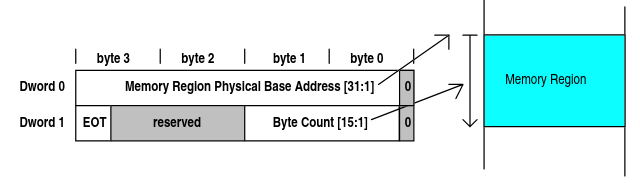
\includegraphics[scale=0.8]{../figures/prd.png}
		\end{center}
		Notiamo che le regioni indicate dall'indirizzo base dell'entrata PRD può essere al massimo di 64 KiB. Per questo lato hardware si può usare un sommatore a sole 16 cifre.
		In ogni caso, questo non sarà un problema in quanto vorremo trasferire buffer in memoria virtuale una pagina (4 KiB) alla volta.
\end{itemize}

A questo punto basterà definire i passaggi di un operazione di trasferimento:
\begin{enumerate}
	\item Si prepara una tabella PRD in memoria;
	\item Si carica l'indirizzo base della tabella PRD nel registro BMDTPR, quindi si ripuliscono i bit di interruzione ed errore del registro di stato BMSTR;
	\item Si fornisce il comando appropiato sul registro BMCMD;
	\item Si attiva il bit 0 del registro BMCMD per attivare il bus mastering;
	\item Il controllore DMA trasferisce i dati secondo quanto disposto finora;
	\item Alla fine della trasmissione il controllore segnala la fine dell'operazione su una linea di interruzinoe;
	\item In risposta all'interruzione, si resetta il bit 0 del registro BMCMD, e si legge lo stato dal controllore e dal disco per capire se l'operazione è andata a buon fine.
\end{enumerate}

\par\smallskip

Vediamo quindi un semplice programma, che reinterpreta effettivamente quanto fatto in 4.1, usando il controllore DMA anzichè il controllo programma per effettuare gli accessi al disco rigido.
Altre modifiche sono state fatte rispetto all'esempio in 4.1 per usare il più possibile le utilità fornite da \lstinline|libce|.
\lstset{language=C++,style=codestyle}
\lstinputlisting{../code/interfaces/bm_disk/bm_disk.cpp}

La tabella PRD e il buffer hanno dei prerequisiti particolari sui confini che possono attraversare:
\begin{itemize}
	\item Le entrate PRD devono essere di 8 byte allineate ai 4 byte;
	\item Il buffer deve essere allineato ai 2 byte, e non attraversare confini allineati ai 64 KiB.
\end{itemize}
Per questo motivo li definiamo in un file a parte, in assembler, \lstinline|buffer.s|:
\lstset{language=assembler,style=codestyle}
\lstinputlisting{../code/interfaces/bm_disk/buffer.s}

Infine, definiamo a parte anche la parte assembler del gestore d'interuzione \lstinline|a_int|:
\lstinputlisting{../code/interfaces/bm_disk/bm_disk.s}

\subsubsection{Controller IDE su bus PCI}
Per l'inserzione di un controllore di questo tipo in un bus PCI dobbiamo renderci conto di alcuni dettagli:
Nei registri dello spazio di configurazione del dispositivo si devono attivare dei flag particolari per segnalare la possibilità che questo lavori in bus mastering.

\subsubsection{Controller IDE nel kernel}
Vediamo infine come il controllore DMA dell'hard disk ATA viene gestito nel kernel.
La libreria \lstinline|libce| definisce i registri del controllore:
\begin{lstlisting}[language=C++, style=codestyle]	
namespace bm {
	extern ioaddr iBMCMD; // Bus Master Command
	extern ioaddr iBMSTR; // Bus Master Status Register
	extern ioaddr iBMDTPR; // Bus Master Descriptor Table Pointer
}
\end{lstlisting}
e le relative funzioni per l'inizializzazione, l'acknowledge, ecc...

L'unica interfaccia ATA montata nel sistema è quindi descritta dal descrittore:
\begin{lstlisting}[language=C++, style=codestyle]	
// descrittore di interfaccia ATA
struct des_ata {
	// Ultimo comando inviato all'interfaccia
	natb comando;
	// Indice di un semaforo di mutua esclusione
	natl mutex;
	// Indice di un semaforo di sincronizzazione
	natl sincr;
	// Quanti settori resta da leggere o scrivere
	natb cont;
	// Da dove leggere/dove scrivere il prossimo settore
	natb* punt;
	// Array dei descrittori per il Bus Mastering
	natl* prd;
};
\end{lstlisting}
che tiene conto dell'operazione corrente.

A questo punto il processo esterno dedicato all'hard disk dovrà limitarsi ad inviare i comandi corretti seguendo la scaletta appena riportata.
Unica parte di interesse è quella della preparazione della tabella PRD, per cui bisogna tenere conto che il controllore DMA necessita di indirizzi fisici, e che legge sequenzialmente a partire da tali indirizzi fisici (perciò non si possono superare i 4 KiB della dimensione di pagina).
Per fare questo, e tenere conto di buffer in memoria che iniziano potenzialmente a metà pagina, si sfrutta la funzione \lstinline|prepare_prd()|:
\begin{lstlisting}[language=C++, style=codestyle]	
bool prepare_prd(des_ata *d, natb* vett, natb quanti)
{
	// ottieni il numero di byte da trasferire
	natq n = quanti * DIM_BLOCK;

	int i = 0;

	// scorri
	while (n && i < MAX_PRD) {
		// ottieni l'indirizzo fisico dell'indirizzo corrente
		paddr p = trasforma(vett);

		// otteni il numero di byte nella pagina corrente
		// sarebbe dimensione_pagina - scarto
		natq  r = DIM_PAGINA - (p % DIM_PAGINA);
		
		// se eccede il numero di byte, taglia
		if (r > n)
			r = n;

		// imposta l'entrata PRD
		d->prd[i] = p;
		d->prd[i + 1] = r;
		
		// rimuovi da n il numero di byte presi
		n -= r;
		// avanza il vettore del numero di byte presi
		vett += r;

		// passa alla prossima entrata PRD
		i += 2;
	}

	// se non hai coperto tutti i byte e' errore
	if (n)
		return false;
	
	// imposta il bit end of table
	d->prd[i - 1] |= 0x80000000;
	return true;
}
\end{lstlisting}
Un dettaglio interessante è che si usa la \lstinline|trasforma()| per ogni entrata PRD che si va a generare, in quanto chiaramente ognuna di queste avrà bisogno di un nuovo indirizzo fisico.
Per questo motivo si mantiene oltre al numero di byte mancanti anche l'indirizzo corrente all'interno del vettore (in \lstinline|vett|).

A questo punto si possono fornire all'utente primitive per l'accesso all'hard disk sia a controllo interruzione (come avevamo già visto, implementato in \lstinline|libce|) sia in DMA.
Queste saranno:
\begin{itemize}
	\item \textbf{Controllo interruzione:} vediamo ad esempio l'operazione di ingresso.
\begin{lstlisting}[language=C++, style=codestyle]	
// fondamentalmente un wrapper per hd::start_cmd di libce, che aggiorna il descrittore
void starthd_in(des_ata* d, natb vetti[], natl primo, natb quanti)
{
	d->cont = quanti;
	d->punt = vetti;
	d->comando = hd::READ_SECT;
	hd::start_cmd(primo, quanti, hd::READ_SECT);
}

// la primitiva vera e propria
extern "C" void c_readhd_n(natb vetti[], natl primo, natb quanti)
{
	des_ata* d = &hard_disk;

	// controlli (c_access)

	sem_wait(d->mutex);
	starthd_in(d, vetti, primo, quanti);
	sem_wait(d->sincr);
	sem_signal(d->mutex);
}
\end{lstlisting}
\item \textbf{DMA:} vediamo sempre l'operazione di ingresso:
\begin{lstlisting}[language=C++, style=codestyle]	
void dmastarthd_in(des_ata* d, natb vetti[], natl primo, natb quanti)
{
	// passo 1 della scaletta
	if (!prepare_prd(d, vetti, quanti)) {
		flog(LOG_ERR, "dmastarthd_in: numero di PRD insufficiente");
		sem_signal(d->sincr);
		return;
	}

	d->comando = hd::READ_DMA;
	d->cont = 1;

	// passo 2
	paddr prd = trasforma(d->prd);
	bm::prepare(prd, false);
	
	// passo 3
	hd::start_cmd(primo, quanti, hd::READ_DMA);
	bm::start();
}
\end{lstlisting}
\end{itemize}

A operazioni terminate, il processo esterno dovrà chiaramente interpretare correttamente le interruzoni che riceve in base al tipo di comando dato:
\begin{lstlisting}[language=C++, style=codestyle]	
void estern_hd(natq)
{
	des_ata* d = &hard_disk;
	for(;;) {
		d->cont--;
		hd::ack();
		switch (d->comando) {
		// questi sono i casi gia visti
		case hd::READ_SECT:
			hd::input_sect(d->punt);
			d->punt += DIM_BLOCK;
			break;
		case hd::WRITE_SECT:
			if (d->cont != 0) {
				hd::output_sect(d->punt);
				d->punt += DIM_BLOCK;
			}
			break;
		case hd::READ_DMA:
		case hd::WRITE_DMA:
			// qui si fa l'acknowledge, passo 7 della scaletta
			bm::ack();
			break;
		}
		if (d->cont == 0)
			sem_signal(d->sincr);
		wfi();
	}
}
\end{lstlisting}

\end{document}


\documentclass[a4paper,11pt]{article}
\usepackage[a4paper, margin=8em]{geometry}

% usa i pacchetti per la scrittura in italiano
\usepackage[french,italian]{babel}
\usepackage[T1]{fontenc}
\usepackage[utf8]{inputenc}
\frenchspacing 

% usa i pacchetti per la formattazione matematica
\usepackage{amsmath, amssymb, amsthm, amsfonts}

% usa altri pacchetti
\usepackage{gensymb}
\usepackage{hyperref}
\usepackage{standalone}

\usepackage{colortbl}

\usepackage{xstring}
\usepackage{karnaugh-map}

% imposta il titolo
\title{Appunti Calcolatori Elettronici}
\author{Luca Seggiani}
\date{2025}

% imposta lo stile
% usa helvetica
\usepackage[scaled]{helvet}
% usa palatino
\usepackage{palatino}
% usa un font monospazio guardabile
\usepackage{lmodern}

\renewcommand{\rmdefault}{ppl}
\renewcommand{\sfdefault}{phv}
\renewcommand{\ttdefault}{lmtt}

% circuiti
\usepackage{circuitikz}
\usetikzlibrary{babel}

% testo cerchiato
\newcommand*\circled[1]{\tikz[baseline=(char.base)]{
\node[shape=circle,draw,inner sep=2pt] (char) {#1};}}

% disponi il titolo
\makeatletter
\renewcommand{\maketitle} {
	\begin{center} 
		\begin{minipage}[t]{.8\textwidth}
			\textsf{\huge\bfseries \@title} 
		\end{minipage}%
		\begin{minipage}[t]{.2\textwidth}
			\raggedleft \vspace{-1.65em}
			\textsf{\small \@author} \vfill
			\textsf{\small \@date}
		\end{minipage}
		\par
	\end{center}

	\thispagestyle{empty}
	\pagestyle{fancy}
}
\makeatother

% disponi teoremi
\usepackage{tcolorbox}
\newtcolorbox[auto counter, number within=section]{theorem}[2][]{%
	colback=blue!10, 
	colframe=blue!40!black, 
	sharp corners=northwest,
	fonttitle=\sffamily\bfseries, 
	title=Teorema~\thetcbcounter: #2, 
	#1
}

% disponi definizioni
\newtcolorbox[auto counter, number within=section]{definition}[2][]{%
	colback=red!10,
	colframe=red!40!black,
	sharp corners=northwest,
	fonttitle=\sffamily\bfseries,
	title=Definizione~\thetcbcounter: #2,
	#1
}

% disponi codice
\usepackage{listings}
\usepackage[table]{xcolor}

\definecolor{codegreen}{rgb}{0,0.6,0}
\definecolor{codegray}{rgb}{0.5,0.5,0.5}
\definecolor{codepurple}{rgb}{0.58,0,0.82}
\definecolor{backcolour}{rgb}{0.95,0.95,0.92}

\lstdefinestyle{codestyle}{
	backgroundcolor=\color{black!5}, 
	commentstyle=\color{codegreen},
	keywordstyle=\bfseries\color{magenta},
	numberstyle=\sffamily\tiny\color{black!60},
	stringstyle=\color{green!50!black},
	basicstyle=\ttfamily\footnotesize,
	breakatwhitespace=false,         
	breaklines=true,                 
	captionpos=b,                    
	keepspaces=true,                 
	numbers=left,                    
	numbersep=5pt,                  
	showspaces=false,                
	showstringspaces=false,
	showtabs=false,                  
	tabsize=2
}

\lstdefinestyle{shellstyle}{
	backgroundcolor=\color{black!5}, 
	basicstyle=\ttfamily\footnotesize\color{black}, 
	commentstyle=\color{black}, 
	keywordstyle=\color{black},
	numberstyle=\color{black!5},
	stringstyle=\color{black}, 
	showspaces=false,
	showstringspaces=false, 
	showtabs=false, 
	tabsize=2, 
	numbers=none, 
	breaklines=true
}


\lstdefinelanguage{assembler}{ 
	keywords={AAA, AAD, AAM, AAS, ADC, ADCB, ADCW, ADCL, ADD, ADDB, ADDW, ADDL, AND, ANDB, ANDW, ANDL,
		ARPL, BOUND, BSF, BSFL, BSFW, BSR, BSRL, BSRW, BSWAP, BT, BTC, BTCB, BTCW, BTCL, BTR, 
		BTRB, BTRW, BTRL, BTS, BTSB, BTSW, BTSL, CALL, CBW, CDQ, CLC, CLD, CLI, CLTS, CMC, CMP,
		CMPB, CMPW, CMPL, CMPS, CMPSB, CMPSD, CMPSW, CMPXCHG, CMPXCHGB, CMPXCHGW, CMPXCHGL,
		CMPXCHG8B, CPUID, CWDE, DAA, DAS, DEC, DECB, DECW, DECL, DIV, DIVB, DIVW, DIVL, ENTER,
		HLT, IDIV, IDIVB, IDIVW, IDIVL, IMUL, IMULB, IMULW, IMULL, IN, INB, INW, INL, INC, INCB,
		INCW, INCL, INS, INSB, INSD, INSW, INT, INT3, INTO, INVD, INVLPG, IRET, IRETD, JA, JAE,
		JB, JBE, JC, JCXZ, JE, JECXZ, JG, JGE, JL, JLE, JMP, JNA, JNAE, JNB, JNBE, JNC, JNE, JNG,
		JNGE, JNL, JNLE, JNO, JNP, JNS, JNZ, JO, JP, JPE, JPO, JS, JZ, LAHF, LAR, LCALL, LDS,
		LEA, LEAVE, LES, LFS, LGDT, LGS, LIDT, LMSW, LOCK, LODSB, LODSD, LODSW, LOOP, LOOPE,
		LOOPNE, LSL, LSS, LTR, MOV, MOVB, MOVW, MOVL, MOVSB, MOVSD, MOVSW, MOVSX, MOVSXB,
		MOVSXW, MOVSXL, MOVZX, MOVZXB, MOVZXW, MOVZXL, MUL, MULB, MULW, MULL, NEG, NEGB, NEGW,
		NEGL, NOP, NOT, NOTB, NOTW, NOTL, OR, ORB, ORW, ORL, OUT, OUTB, OUTW, OUTL, OUTSB, OUTSD,
		OUTSW, POP, POPL, POPW, POPB, POPA, POPAD, POPF, POPFD, PUSH, PUSHL, PUSHW, PUSHB, PUSHA, 
		PUSHAD, PUSHF, PUSHFD, RCL, RCLB, RCLW, MOVSL, MOVSB, MOVSW, STOSL, STOSB, STOSW, LODSB, LODSW,
		LODSL, INSB, INSW, INSL, OUTSB, OUTSL, OUTSW
		RCLL, RCR, RCRB, RCRW, RCRL, RDMSR, RDPMC, RDTSC, REP, REPE, REPNE, RET, ROL, ROLB, ROLW,
		ROLL, ROR, RORB, RORW, RORL, SAHF, SAL, SALB, SALW, SALL, SAR, SARB, SARW, SARL, SBB,
		SBBB, SBBW, SBBL, SCASB, SCASD, SCASW, SETA, SETAE, SETB, SETBE, SETC, SETE, SETG, SETGE,
		SETL, SETLE, SETNA, SETNAE, SETNB, SETNBE, SETNC, SETNE, SETNG, SETNGE, SETNL, SETNLE,
		SETNO, SETNP, SETNS, SETNZ, SETO, SETP, SETPE, SETPO, SETS, SETZ, SGDT, SHL, SHLB, SHLW,
		SHLL, SHLD, SHR, SHRB, SHRW, SHRL, SHRD, SIDT, SLDT, SMSW, STC, STD, STI, STOSB, STOSD,
		STOSW, STR, SUB, SUBB, SUBW, SUBL, TEST, TESTB, TESTW, TESTL, VERR, VERW, WAIT, WBINVD,
	XADD, XADDB, XADDW, XADDL, XCHG, XCHGB, XCHGW, XCHGL, XLAT, XLATB, XOR, XORB, XORW, XORL},
	keywordstyle=\color{blue}\bfseries,
	ndkeywordstyle=\color{darkgray}\bfseries,
	identifierstyle=\color{black},
	sensitive=false,
	comment=[l]{\#},
	morecomment=[s]{/*}{*/},
	commentstyle=\color{purple}\ttfamily,
	stringstyle=\color{red}\ttfamily,
	morestring=[b]',
	morestring=[b]"
}

\lstset{language=assembler, style=codestyle}

% disponi sezioni
\usepackage{titlesec}

\titleformat{\section}
{\sffamily\Large\bfseries} 
{\thesection}{1em}{} 
\titleformat{\subsection}
{\sffamily\large\bfseries}   
{\thesubsection}{1em}{} 
\titleformat{\subsubsection}
{\sffamily\normalsize\bfseries} 
{\thesubsubsection}{1em}{}

% tikz
\usepackage{tikz}

% float
\usepackage{float}

% grafici
\usepackage{pgfplots}
\pgfplotsset{width=10cm,compat=1.9}

% disponi alberi
\usepackage{forest}

\forestset{
	rectstyle/.style={
		for tree={rectangle,draw,font=\large\sffamily}
	},
	roundstyle/.style={
		for tree={circle,draw,font=\large}
	}
}

% disponi algoritmi
\usepackage{algorithm}
\usepackage{algorithmic}
\makeatletter
\renewcommand{\ALG@name}{Algoritmo}
\makeatother

% disponi numeri di pagina
\usepackage{fancyhdr}
\fancyhf{} 
\fancyfoot[L]{\sffamily{\thepage}}

\makeatletter
\fancyhead[L]{\raisebox{1ex}[0pt][0pt]{\sffamily{\@title \ \@date}}} 
\fancyhead[R]{\raisebox{1ex}[0pt][0pt]{\sffamily{\@author}}}
\makeatother

\begin{document}
% sezione (data)
\section{Lezione del 05-05-25}

% stili pagina
\thispagestyle{empty}
\pagestyle{fancy}

% testo
\subsection{Architettura interna del processore}
Vediamo più nel dettaglio dell'architettura interna dei processori Intel x86.

Per velocizzare l'operazione del processo la via principale potrebbe essere quello di aumentare  le prestazioni dei componenti, cioè dei transistor, che lo compongono.
Si ha che questo approccio però non è scalabile all'infinito, in quanto negli ultimi anni si è raggiunto un \textit{plateu} delle prestazioni.

La soluzione che vediamo è quindi \textbf{architetturale}, e consiste nell'uso di una \textbf{pipeline} particolare per l'esecuzione delle istruzioni.
Un normale ciclo di esecuzione di un'istruzione si svolge come:

\begin{table}[h!]
	\center \rowcolors{2}{white}{black!10}
	\begin{tabular} { c | c | c | c | c }
		\sffamily Prelievo istruzione & \sffamily Decodifica & \sffamily Prelievo operandi & \sffamily Esecuzione & \sffamily Scrittura
	\end{tabular}
\end{table}

\subsubsection{Pipeline}
Se ognuna di queste fasi è svolta da una certa circuiteria, possiamo far passare in parallelo ogni istruzione da ogni circuiteria, cioè avere che l'istruzione gestita ad ogni istante temporale sucessivo $t_0$, $t_1$, ... è:

\begin{table}[h!]
	\center \rowcolors{2}{white}{black!10}
	\begin{tabular} { c |c | c | c | c | c }
		& \sffamily Prelievo istruzione & \sffamily Decodifica & \sffamily Prelievo operandi & \sffamily Esecuzione & \sffamily Scrittura \\
		\hline
		$t_0$ & $i$ & & & & \\
		$t_1$ & $i + 1$ & $i$ & & & \\
		$t_2$ & $i + 2$ & $i + 1$ & $i$ & &  \\
		$t_3$ & $i + 3$ & $i + 2$ & $i + 1$ & $i$ & \\
		$t_4$ & $i + 4$ & $i + 3$ & $i + 2$ & $i + 1$ & $i$ \\
	\end{tabular}
\end{table}

Questo approccio chiaramente non modifica il tempo necessario ad eseguire una istruzione (e anzi vedremo lo aumenta un po'), ma di contro permette di aumentare la frequenza delle istruzioni eseguite, per l'esattezza di un fattore pari al numero di fasi in cui si divide l'esecuzione (qui 5).

Realizzaremo infatti questo tipo di struttura frapponendo fra ogni blocco funzionale un registro, che campiona sul rising edge del clock, rallentando leggermente la velocità della pipeline per accomodare il tempo di setup dei registri.
Inoltre, il periodo del clock dovrà essere determinato dal più lungo dei percorsi (in termini temporali) $\Delta_1$, $\Delta_2$, ..., $\Delta_5$ fra un registro e un altro, cioè dall'elemento più lento della pipeline.
Si avrà quindi una configurazione del tipo:
\begin{center}
	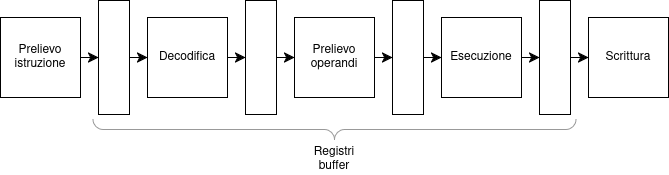
\includegraphics[scale=0.6]{../figures/pipeline.png}
\end{center}
Di base, questa configurazione risulterà comunque un'accelerazione del clock.
Infatti, se l'intera pipeline richiedeva prima un tempo $\Delta$, ci aspettiamo che ogni componente in cui la dividiamo richieda un tempo nell'ordine di $\sim \frac{\Delta}{5}$, ed esattamente $\frac{\Delta}{5}$ se ogni circuiteria ha lo stesso tempo di attraversamento, per cui il clock può essere accelerato di un fattore di $5$.

Il bottleneck è però chiaro per la fase di esecuzione, che potrebbe andare dalla somma naturale alla divisione in virgola mobile, con evidenti differenze in tempo di esecuzione.

Inoltre, la stessa fase di prelievo potrebbe variare in requisiti temporali per via del tipo di codifica delle istruzioni, a lunghezza variabile, adottata dai processori Intel x86 (instruction set \textbf{CISC}, \textit{Complex Instruction Set Computer}, contro gli instruction set \textbf{RISC}, \textit{Reduced Instruction Set Computer}, adottati da ARM).

Ci troveremo quindi di fronte a situazioni dove, con una sola circuiteria di prelievo, non si può sapere quando un'istruzione è veramente finita prima di decodificarla, e quindi non si può procedere con una nuova fase di prelievo.

Chiaramente, tutto questo procedimento è semplificato per i processori ad architettura RISC, in quanto la dimensione delle istruzioni è standardizzata.
Inoltre, si ottengono vantaggi nella gestione della pipeline eliminando la possibilità di avere operandi in memoria: si dedicano istruzioni dedicate alla lettura/scrittura in memoria da registri, cioe le \lstinline|LOAD| e \lstinline|STORE|, più semplici da gestire. 

\subsubsection{Alee}

Altri problemi sono dati dalle \textbf{alee}, cioè legati ai salti condizionali (\textit{alee di controllo}), o a casi dove istruzioni hanno bisogno di risultati di istruzioni ancora in pipeline (\textit{alee di dati}), se non a casi dove la pipeline non permette in primo luogo l'esecuzione successiva di due istruzioni (\textit{alee strutturali}).

\begin{itemize}
	\item 
		Questi problemi possono sempre essere risolti dall'introduzione di \textbf{bolle}: si modificano i registri intermedi perché possano conservare il loro stato, e in caso una certa rete di controllo rilevi situazioni a rischio di alee, si introducono nella pipeline \textit{bolle}, cioè si lasciano stadi di elaborazione vuoti, o se vogliamo si introducono istruzioni \lstinline|nop|, a effetto nullo (che chiaramente rappresentano throughput spreacto).
		I registri che alimentano gli stadi rimasti in attesa manterranno quindi una copia dell'istruzione allo scorso ciclo di clock, e invieranno invece avanti istruzioni nulle.
		In questo modo si torna effettivamente al processore prima della pipeline.
	\item 
		Un'altra soluzione per alee dati e alee strutturali può essere quella di dotare l'ultima fase della pipeline di una linea di \textbf{bypass}, che porti il risultato a termine esecuzione a fronte della fase di esecuzione: un istruzione che richiede un operando non ancora scritto dall'istruzione precedente può ottenerlo direttamente da questa, attraverso il bypass.

	\item 
		Per la gestione delle alee di controllo possiamo sfruttare la cosiddetta \textit{esecuzione predittiva}, in particolare \textbf{branch prediction}: si fa un ipotesi sul risultato dell'istruzione di salto condizionale, e si riempie la pipeline con istruzioni che provengono dalla regione corrispondente di programma.
		Al momento della fase di esecuzione dell'istruzione di salto, si capisce quindi se l'ipotesi si è avverata o meno, e si procede ripulendola completamente introducendo bolle (in caso di \textit{miss}, pagando un prezzo pari al numero di fasi della pipeline) o non facendo nulla (in caso di \textit{hit}).

		Esistono politiche leggermente diverse in caso di salti \textbf{diretti} (con indirizzo noto) o \textbf{indiretti} (ad indirizzi calcolati).

		\begin{itemize}
			\item 
				\textbf{Salti diretti}: in questo caso si fa una predizione \textbf{statica}, cioè si sceglie sostanzialmente a caso fra gli esiti del salto.
				Esistono comunque alcune euristiche che possiamo usare: nel caso di salti \textit{all'indietro} ci si aspetta di entrare in un loop, e quindi si assume che il salto verrà eseguito; di contro per salti \textit{in avanti} l'ipotesi è meno forte e ci si aspetta che il salto non verrà eseguito. 

				\newpage

				Abbiamo quindi a grandi linee la struttura funzionale:
				\begin{center}
					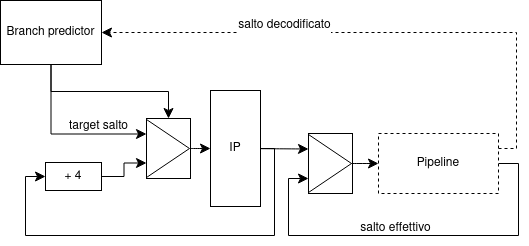
\includegraphics[scale=.65]{../figures/branch_static.png}
				\end{center}
				dove una qualche rete di branch prediction valuta le regole appena valutate per ogni istruzione di salto decodificata dalla pipeline, e invia al primo stadio della pipeline stessa la prossima istruzione che ne ricava. 
				Notiamo che il $+4$ corrisponde al calcolo dell'indirizzo della prossima istruzione sequenziale: si assume che l'architettura abbia istruzioni RISC fisse a 4 byte (vedremo che nelle architetture moderne la semplificazione non è inopportuna).

			\item 
				\textbf{Salti indiretti:} Per questi ci si aspetta che i salti si comporteranno come si sono comportati in precedenza, cioè si fa una predizione \textbf{dinamica}.
				Questo compito è associato ad una componente detta \textbf{BTB}, \textit{Branch Target Buffer}, che si occupa di capire se un salto verrà effettuato o meno sulla base della sua storia precedente, e a quale locazione si salterà, sempre basandosi sulla storia precedente, nel caso di salti indiretti.

				Questi circuiti assumono essenzialmente la forma di cache, e visto che il loro insuccesso (\textit{miss}) risulta solo in un annullamento di un ciclo di pipeline, non si preoccupano di gestire le collisioni.

				In questo caso la struttura funzionale è del tipo:
				\begin{center}
					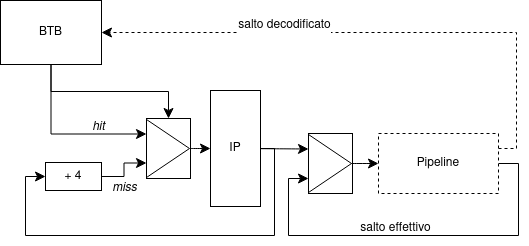
\includegraphics[scale=.65]{../figures/branch_dynamic.png}
				\end{center}
				cioè sostanzialmente analoga alla precedente ma dove l'ipotesi sul prossimo salto viene fatta dall'hit/miss della cache BTB.

Si ha che nelle architetture moderne l'approccio adottato effettivamente è quello del BTB, sia per i salti diretti che i salti indiretti.
Chiaramente ci saranno differenze strutturali specifiche per le informazioni che sarà necessario memorizzare per entrambi i tipi di salto: se per i salti indiretti è fondamentale ricordare l'indirizzo di arrivo, per i salti diretti basterà ricordare se il salto è stato effettuato o meno.
In ogni caso, può essere utile conservare anche l'indirizzo di arrivo per questioni di ottimizzazione: l'indirizzo potrebbe sì essere ricavato dall'istruzione, ma questo richiederebbe la sua decodifica, mentre il prefetch può iniziare prima ricavando l'indirizzo di arrivo direttamente dall'indirizzod dell'istruzione.
		\end{itemize}

\end{itemize}

\subsubsection{Architettura del Pentium Pro}
Nei processori di oggi, la gestione della pipeline è effettivamente quella che Intel sviluppa dal Pentium Pro del 1995 (che ha continuato ad evolvere fino ad oggi, se non per una deviazione che fu esplorata nel Pentium 4).

In questa architettura, il processore si occupa di tradurre intermante le istruzioni CISC in istruzioni RISC, e quindi a gestire la pipeline con sole istruzioni RISC.
Vorremo quindi rimuovere le fasi di prelievo e decodifica dalla pipeline vista finora, per porle esternamente come parte del ciclo di traduzione da CISC a RISC, e aspettarci che la pipeline vera e propria si veda arrivare istruzioni già decodificate. 

\par\medskip

Notiamo infine che spesso nemmeno l'esecuzione sequenziale del codice non è necessaria.
Prendendo ad esempio il frammento di codice:
\begin{lstlisting}[language=C++, style=codestyle]	
for(int i = 0; i < 1000; i++) {
	a[i] = v1[i] * v2[i];
}
\end{lstlisting}
potremmo "srotolarlo" in:
\begin{lstlisting}[language=C++, style=codestyle]	
a[0] = v1[0] * v2[0];
a[1] = v1[1] * v2[1];
// ...
a[999] = v1[999] * v2[999];
\end{lstlisting}

\subsubsection{Esecuzione asincrona}
Vediamo che nessuna di queste istruzioni dipende dalle altre, ergo l'ordine in cui vengono eseguite non è importante.
In questo caso il miss di cache per alcune di queste può tradursi semplicemente in un ritardo nella loro esecuzione, mentre altre che invece si trovano in cache (magari relative ad indirizzi successivi) possono essere eseguite da subito, cioè l'esecuzione asincrona è non solo possibile, ma può risultare anche utile.

\subsubsection{Esecuzione predittiva}
Un'ultima tecnica che il processore moderno può usare per accelerare l'esecuzione delle istruzioni è eseguire istruzioni prima che questo sia necessario, eventualmente scartando i risultati nel caso risultino inutili. 

\end{document}


\documentclass[a4paper,11pt]{article}
\usepackage[a4paper, margin=8em]{geometry}

% usa i pacchetti per la scrittura in italiano
\usepackage[french,italian]{babel}
\usepackage[T1]{fontenc}
\usepackage[utf8]{inputenc}
\frenchspacing 

% usa i pacchetti per la formattazione matematica
\usepackage{amsmath, amssymb, amsthm, amsfonts}

% usa altri pacchetti
\usepackage{gensymb}
\usepackage{hyperref}
\usepackage{standalone}

\usepackage{colortbl}

\usepackage{xstring}
\usepackage{karnaugh-map}

% imposta il titolo
\title{Appunti Calcolatori Elettronici}
\author{Luca Seggiani}
\date{2025}

% imposta lo stile
% usa helvetica
\usepackage[scaled]{helvet}
% usa palatino
\usepackage{palatino}
% usa un font monospazio guardabile
\usepackage{lmodern}

\renewcommand{\rmdefault}{ppl}
\renewcommand{\sfdefault}{phv}
\renewcommand{\ttdefault}{lmtt}

% circuiti
\usepackage{circuitikz}
\usetikzlibrary{babel}

% testo cerchiato
\newcommand*\circled[1]{\tikz[baseline=(char.base)]{
\node[shape=circle,draw,inner sep=2pt] (char) {#1};}}

% disponi il titolo
\makeatletter
\renewcommand{\maketitle} {
	\begin{center} 
		\begin{minipage}[t]{.8\textwidth}
			\textsf{\huge\bfseries \@title} 
		\end{minipage}%
		\begin{minipage}[t]{.2\textwidth}
			\raggedleft \vspace{-1.65em}
			\textsf{\small \@author} \vfill
			\textsf{\small \@date}
		\end{minipage}
		\par
	\end{center}

	\thispagestyle{empty}
	\pagestyle{fancy}
}
\makeatother

% disponi teoremi
\usepackage{tcolorbox}
\newtcolorbox[auto counter, number within=section]{theorem}[2][]{%
	colback=blue!10, 
	colframe=blue!40!black, 
	sharp corners=northwest,
	fonttitle=\sffamily\bfseries, 
	title=Teorema~\thetcbcounter: #2, 
	#1
}

% disponi definizioni
\newtcolorbox[auto counter, number within=section]{definition}[2][]{%
	colback=red!10,
	colframe=red!40!black,
	sharp corners=northwest,
	fonttitle=\sffamily\bfseries,
	title=Definizione~\thetcbcounter: #2,
	#1
}

% disponi codice
\usepackage{listings}
\usepackage[table]{xcolor}

\definecolor{codegreen}{rgb}{0,0.6,0}
\definecolor{codegray}{rgb}{0.5,0.5,0.5}
\definecolor{codepurple}{rgb}{0.58,0,0.82}
\definecolor{backcolour}{rgb}{0.95,0.95,0.92}

\lstdefinestyle{codestyle}{
	backgroundcolor=\color{black!5}, 
	commentstyle=\color{codegreen},
	keywordstyle=\bfseries\color{magenta},
	numberstyle=\sffamily\tiny\color{black!60},
	stringstyle=\color{green!50!black},
	basicstyle=\ttfamily\footnotesize,
	breakatwhitespace=false,         
	breaklines=true,                 
	captionpos=b,                    
	keepspaces=true,                 
	numbers=left,                    
	numbersep=5pt,                  
	showspaces=false,                
	showstringspaces=false,
	showtabs=false,                  
	tabsize=2
}

\lstdefinestyle{shellstyle}{
	backgroundcolor=\color{black!5}, 
	basicstyle=\ttfamily\footnotesize\color{black}, 
	commentstyle=\color{black}, 
	keywordstyle=\color{black},
	numberstyle=\color{black!5},
	stringstyle=\color{black}, 
	showspaces=false,
	showstringspaces=false, 
	showtabs=false, 
	tabsize=2, 
	numbers=none, 
	breaklines=true
}


\lstdefinelanguage{assembler}{ 
	keywords={AAA, AAD, AAM, AAS, ADC, ADCB, ADCW, ADCL, ADD, ADDB, ADDW, ADDL, AND, ANDB, ANDW, ANDL,
		ARPL, BOUND, BSF, BSFL, BSFW, BSR, BSRL, BSRW, BSWAP, BT, BTC, BTCB, BTCW, BTCL, BTR, 
		BTRB, BTRW, BTRL, BTS, BTSB, BTSW, BTSL, CALL, CBW, CDQ, CLC, CLD, CLI, CLTS, CMC, CMP,
		CMPB, CMPW, CMPL, CMPS, CMPSB, CMPSD, CMPSW, CMPXCHG, CMPXCHGB, CMPXCHGW, CMPXCHGL,
		CMPXCHG8B, CPUID, CWDE, DAA, DAS, DEC, DECB, DECW, DECL, DIV, DIVB, DIVW, DIVL, ENTER,
		HLT, IDIV, IDIVB, IDIVW, IDIVL, IMUL, IMULB, IMULW, IMULL, IN, INB, INW, INL, INC, INCB,
		INCW, INCL, INS, INSB, INSD, INSW, INT, INT3, INTO, INVD, INVLPG, IRET, IRETD, JA, JAE,
		JB, JBE, JC, JCXZ, JE, JECXZ, JG, JGE, JL, JLE, JMP, JNA, JNAE, JNB, JNBE, JNC, JNE, JNG,
		JNGE, JNL, JNLE, JNO, JNP, JNS, JNZ, JO, JP, JPE, JPO, JS, JZ, LAHF, LAR, LCALL, LDS,
		LEA, LEAVE, LES, LFS, LGDT, LGS, LIDT, LMSW, LOCK, LODSB, LODSD, LODSW, LOOP, LOOPE,
		LOOPNE, LSL, LSS, LTR, MOV, MOVB, MOVW, MOVL, MOVSB, MOVSD, MOVSW, MOVSX, MOVSXB,
		MOVSXW, MOVSXL, MOVZX, MOVZXB, MOVZXW, MOVZXL, MUL, MULB, MULW, MULL, NEG, NEGB, NEGW,
		NEGL, NOP, NOT, NOTB, NOTW, NOTL, OR, ORB, ORW, ORL, OUT, OUTB, OUTW, OUTL, OUTSB, OUTSD,
		OUTSW, POP, POPL, POPW, POPB, POPA, POPAD, POPF, POPFD, PUSH, PUSHL, PUSHW, PUSHB, PUSHA, 
		PUSHAD, PUSHF, PUSHFD, RCL, RCLB, RCLW, MOVSL, MOVSB, MOVSW, STOSL, STOSB, STOSW, LODSB, LODSW,
		LODSL, INSB, INSW, INSL, OUTSB, OUTSL, OUTSW
		RCLL, RCR, RCRB, RCRW, RCRL, RDMSR, RDPMC, RDTSC, REP, REPE, REPNE, RET, ROL, ROLB, ROLW,
		ROLL, ROR, RORB, RORW, RORL, SAHF, SAL, SALB, SALW, SALL, SAR, SARB, SARW, SARL, SBB,
		SBBB, SBBW, SBBL, SCASB, SCASD, SCASW, SETA, SETAE, SETB, SETBE, SETC, SETE, SETG, SETGE,
		SETL, SETLE, SETNA, SETNAE, SETNB, SETNBE, SETNC, SETNE, SETNG, SETNGE, SETNL, SETNLE,
		SETNO, SETNP, SETNS, SETNZ, SETO, SETP, SETPE, SETPO, SETS, SETZ, SGDT, SHL, SHLB, SHLW,
		SHLL, SHLD, SHR, SHRB, SHRW, SHRL, SHRD, SIDT, SLDT, SMSW, STC, STD, STI, STOSB, STOSD,
		STOSW, STR, SUB, SUBB, SUBW, SUBL, TEST, TESTB, TESTW, TESTL, VERR, VERW, WAIT, WBINVD,
	XADD, XADDB, XADDW, XADDL, XCHG, XCHGB, XCHGW, XCHGL, XLAT, XLATB, XOR, XORB, XORW, XORL},
	keywordstyle=\color{blue}\bfseries,
	ndkeywordstyle=\color{darkgray}\bfseries,
	identifierstyle=\color{black},
	sensitive=false,
	comment=[l]{\#},
	morecomment=[s]{/*}{*/},
	commentstyle=\color{purple}\ttfamily,
	stringstyle=\color{red}\ttfamily,
	morestring=[b]',
	morestring=[b]"
}

\lstset{language=assembler, style=codestyle}

% disponi sezioni
\usepackage{titlesec}

\titleformat{\section}
{\sffamily\Large\bfseries} 
{\thesection}{1em}{} 
\titleformat{\subsection}
{\sffamily\large\bfseries}   
{\thesubsection}{1em}{} 
\titleformat{\subsubsection}
{\sffamily\normalsize\bfseries} 
{\thesubsubsection}{1em}{}

% tikz
\usepackage{tikz}

% float
\usepackage{float}

% grafici
\usepackage{pgfplots}
\pgfplotsset{width=10cm,compat=1.9}

% disponi alberi
\usepackage{forest}

\forestset{
	rectstyle/.style={
		for tree={rectangle,draw,font=\large\sffamily}
	},
	roundstyle/.style={
		for tree={circle,draw,font=\large}
	}
}

% disponi algoritmi
\usepackage{algorithm}
\usepackage{algorithmic}
\makeatletter
\renewcommand{\ALG@name}{Algoritmo}
\makeatother

% disponi numeri di pagina
\usepackage{fancyhdr}
\fancyhf{} 
\fancyfoot[L]{\sffamily{\thepage}}

\makeatletter
\fancyhead[L]{\raisebox{1ex}[0pt][0pt]{\sffamily{\@title \ \@date}}} 
\fancyhead[R]{\raisebox{1ex}[0pt][0pt]{\sffamily{\@author}}}
\makeatother

\begin{document}
% sezione (data)
\section{Lezione del 06-05-25}

% stili pagina
\thispagestyle{empty}
\pagestyle{fancy}

% testo
Riprendiamo più nel dettaglio i concetti che abbiamo solamente accennatto alla scorsa lezione.

\subsubsection{Ordinamento delle istruzioni}
Abbiamo che l'\textit{ordinamento totale} delle istruzioni del programma è solo un artefatto di come questo è compilato: non necessariamente le istruzioni vanno eseguite in tale ordine per arrivare allo stesso risultato finale.

Le istruzioni si trovano infatti solo in un \textit{ordinamento parziale}, dove solo alcune istruzioni hanno bisogno, per motivi di sincronia, di essere eseguite successivamente ad altre.

Prendiamo quindi l'esempio \lstinline|op1, src1, sec2, dst|, con sintassi simile all'assembly ARM (e in generale delle istruzioni RISC, dove ricordiamo gli operandi sono sempre registri). # da qualche parte fai un discorso ARM - RISC
Una volta che i sorgenti \lstinline|src1| e \lstinline|src2| sono definiti, questa può essere eseguita.

Ipotizziamo quindi un'architettura dove sono previste un numero arbitrario di ALU, preceduta da componenti che denominiamo \textbf{stazioni di prenotazione}, fondamentalmente registri capaci di contenere la codifica macchina di una istruzione.

Ogni istruzione che viene decodificata dal processore viene spostata in una stazione di prenotazione. 
Non appena gli operandi saranno pronti, l'istruzione potrà quindi essere messa in esecuzione.

Viene da sé che questa architettura ci permette di ottenere un'esecuzione delle istruzioni che è \textit{fuori ordine} e in \textit{parallelo}.

\subsubsection{Dipendenze}
Chiaramente, però, resterà da definire le regole secondo le quali le istruzioni devono essere eseguite prima o dopo di altre.
Chiamiamo queste condizioni \textbf{dipendenze}, fra cui distinguiamo:
\begin{itemize}
	\item Dipendenze \textbf{dati};
	\item Dipendenze \textbf{nomi};
	\item Dipendenze \textbf{controllo};
\end{itemize}
dove la prima e l'ultima non vanno confuse con le alee: adesso parliamo di conseguenze di come è fatto il \textit{programma}, non di come è fatto il \textit{processore}.

Le dipendenze \textbf{dati} sono il caso che abbiamo già visto.
Se abbiamo due istruzioni:
\begin{lstlisting}	
add r1, r2, r3
...
sub r4, r3, r5
\end{lstlisting}
si ha che la \lstinline|sub| dipende per dati dalla \lstinline|add|, in quanto questa intacca \lstinline|r3|, operando.

Per ogni registro dovremo quindi mantenere delle informazioni associate: quando una istruzione viene messa in una stazione (si dice viene \textbf{emessa}), si alza un certo flag associato al registro che intaccherà. 
Questo flag viene poi abbassato in fase di esecuzione vera e propria, insieme all'aggiornamento dei dati del registro stesso.
Un istruzione successiva che vuole usare tale registro dovrà quindi controllare tale flag per capire se quell'operando è pronto.

Le dipendenze sui \textbf{nomi} si dividono in due categorie:
\begin{itemize}
	\item \textbf{Antidipendenze}:
	Poniamo di avere le due istruzioni:
\begin{lstlisting}
add r1, r2, r3
...
sub r4, r5, r1
\end{lstlisting}
in questo caso non si può eseguire la \lstinline|sub| prima della \lstinline|add|, in quanto la prima necessita del \textit{vecchio} contenuto di \lstinline|r1|, non quello che avremo dopo la \lstinline|sub|.
Si deve quindi evitare di mettere in attesa la \lstinline|sub| finché la \lstinline|add| non è conosciuta.

Per risolvere questo tipo di dipendenza dovremmo quindi dotare ogni registro, oltre al flag W, un contatore C che conti quante stazioni contengono istruzioni che usano quel registro come sorgente.
Ogni istruzione emessa alza i contatori dei suoi sorgenti, e ogni istruzione eseguita fino in fondo li abbassa.
Avremo quindi che un istruzione potrà scrivere sulla sua destinazione quando il numero di lettori, e quindi il contatore, è pari a 0.

	\item Dipendenze in \textbf{uscita}:
		Poniamo di avere le due istruzioni:
\begin{lstlisting}
add r1, r2, r3
...
sub r4, r5, r3
\end{lstlisting}
che può sembrare strano, ma può succedere nel caso qualcuno usi \lstinline|r3| fra le due istruzioni, o il compilatore lo faccia comunque per motivi di ottimizzazione.
Ad esempio questo succede spesso per quanto riguarda il registro dei flag, che viene aggiornato costantemente ma letto solamente dalle istruzioni di salto. 

Per risolvere questo tipo di dipendenze si controlla il flag associato al registro di uscita prima dell'emissione: in caso questo sia già preso in scrittura si mette l'istruzione in attesa (simile alle bolle che avevamo visto per la pipeline), per poi emetterla solo quando \lstinline|r3| è stato modificato. 
\end{itemize}

Possiamo dire che, date due istruzioni $j$, $i$ da eseguire in quest'ordine, le dipendenze si classificano come nel seguente schema:

#    j   R    W
# i      
# R      --   dati
# W      anti uscita

Le dipendenze sul \textbf{controllo} si verificano quando istruzioni possono o meno essere eseguito sulla base dell'esito di istruzioni di salto.
Ad esempio, preso:
\begin{lstlisting}	
	cmp
	ja fine

	add ...
	sub ...

fine:
	mul ...
\end{lstlisting}
vorremo che le \lstinline|add| e \lstinline|sub| non fossero eseguite in caso positivo della \lstinline|ja|, mentre la \lstinline|mul| venga eseguita comunque.
Chiaramente questo non è facile, in quanto potremmo avere:
\begin{lstlisting}	
	cmp
	ja fine

	add ...
	sub ...

	jmp fine2

fine:
	mul ...

fine2:
\end{lstlisting}
dove la \lstinline|mul| non può essere eseguita comunque, ma questo non si può sapere finché non si entra nel blocco \lstinline|add ... sub|.
Il processore non ha quindi speranze per risolvere il problema, se non assumere \textit{per eccesso} che tutto ciò che viene dopo la jump dipende dalla jump. 

\subsubsection{Traduzione da CISC a RISC}
Vediamo come può essere effettuata la traduzione da un istruzione CISC al corrispondente insieme di istruzioni \lstinline|RISC|.
Prendiamo ad esempio:
\begin{lstlisting}[language=C++, style=codestyle]	
add %rax, 1000(%ebx, %ecx, 8)
\end{lstlisting}
questa dovrà essere tradotta in qualcosa come:
\begin{lstlisting}[language=C++, style=codestyle]	
shl %ecx, $3, tmp1
add %ebx, tmp1, tmp1
ld 1000(tmp1), tmp2
add %rax, tmp2, tmp2
st tmp2, 1000(tmp1)
\end{lstlisting}

Vediamo come abbiamo bisogno di registri dedicati, \lstinline|tmp1| e \lstinline|tmp2|, interni al processore e non accessibili al programmatore.
Questo chiaramente perchè non vogliamo che la trasformazione in RISC delle istruzioni CISC sporchi i registri programmatore.

\subsubsection{Registri fisici}
Dotando il processore di più registri fisici, oltre a quelli programmatore, possiamo rimuovere le dipendenze sui nomi, dette anche \textit{false dipendenze}. 

Questo si fa attraverso il meccanismo di \textbf{rinominazione} dei registri.
Facciamo in modo che ogni registro logico punti ad un registro fisico, con il numero di registri fisici anche maggiore di quello dei registri logici.

Quando il processore incontra un'istruzione, chiama un registro fisico non appena usato come come il registro di uscita (per tutti, non solo per se stesso), e prende i registri fisici puntati dai registri logici sorgenti come registri sorgenti.
Ad esempio, assunto di partire da una mappatura identità, prendiamo l'istruzione:
\begin{lstlisting}	
add r1, r2, r3
\end{lstlisting}
che viene trasformata in:
\begin{lstlisting}	
add f1, f2, f6 # assunto f6 libero
\end{lstlisting}
dove \textit{libero} significa non usati per niente, quindi non puntati e con contatore C e flag W a 0.

Notiamo che questa fase di traduzione si svolge \textit{dopo} la fase di traduzione in RISC effettuata nei componenti addetti alla fetch e decode, e quindi solo in fase di emissione.

Abbiamo quindi rimosso tutti gli stalli necessari alle dipendenze fra i nomi, in quanto ogni istruzione emessa ha come destinazione un registro fisico libero.

Un'istruzione che ha già avuto i suoi registri logici sorgenti tradotti in registri fisici non si preoccupa di ulteriori aggiornamenti ai registri sorgenti, in quanto queste verranno fatte su altri registri, liberi, e non su quelli che lei ha scelto.

\par \medskip

Vediamo quindi come usare il meccanismo di ridenominazione dei registri per risolvere anche gli stalli sulle dipendenze di controllo.

Avevamo già introdotto l'esecuzione speculativa delle istruzioni.
Nella terminologia Intel, questa viene eseguita attraverso un \textbf{Reorder Buffer}.
All'interno del Reorder Buffer viene mantenuta una lista ordinata delle istruzioni, assieme ad un flag che indica che quell'istruzione è terminata (ma non che il risultato è stato scritto!).

Prima di un'istruzione di salto, si possono eseguire e ritirare tutte le istruzioni.
Dopo l'istruzione di salto, immaginiamo che le istruzioni successive vengano eseguite ma non ritirate (scritte nei registri fisici), secondo una predizione fatta come descritto in 24.1.2.
A seguito del salto, potremmo quindi verificare se la predizione è stata corretta: in caso di hit, avremo che potremo ritirare le istruzioni già eseguite, altrimenti dovremo svuotare il Reorder Buffer.

\end{document}

\end{document}